\documentclass[a4paper,11pt]{book}
\textheight 23 cm
\usepackage{amsmath}
\usepackage{amsfonts}
\usepackage{amssymb}
\usepackage{stmaryrd}
\usepackage{makeidx}
\usepackage{times}
%\usepackage{mathptmx}
%Uncomment next line for pdflatex and use includegraphics with eps file
% for latex2html don't use the option [width=\textwidth]
% check that xfig files are exported magnif 100%
\usepackage{pst-plot}
\usepackage{graphicx}
\usepackage{ifpdf}
\ifpdf
 \usepackage[pdftex,colorlinks]{hyperref}
\else
\usepackage{pst-plot}
\fi
%\usepackage{graphics}
%\usepackage{pstricks}
%\def\@evenhead{\thepage\hfill{\footnotesize\textit{\leftmark}}}
%\def\@oddhead{\footnotesize{\textit{\rightmark}}\hfill\thepage}
%\usepackage{hp}
%HEVEA\@def@charset{US-ASCII}
\usepackage[utf8]{inputenc}
\usepackage[T1]{fontenc}
\usepackage[francais]{babel}
\usepackage{latexsym}

\newcommand{\R}{{\mathbb{R}}}
\newcommand{\C}{{\mathbb{C}}}
\newcommand{\Z}{{\mathbb{Z}}}
\newcommand{\N}{{\mathbb{N}}}

%Dans le r\'epertoire {\tt simulation il y a figure1,figure2,figure3,figure4,
%figure5,Asim,Aex,painA,painG (cf apres le \end{document)

\title{Algorithmique et simulation \\ avec {\tt Xcas}}
\makeindex
\author{Ren\'ee De Graeve}
\begin{document}
\maketitle
\chapter{Le tableur}
\section{G\'en\'eralit\'es}
\subsection{Pour ouvrir un niveau contenant un tableur}
Pour avoir un tableur, il faut utiliser le menu {\tt Edit}, puis {\tt Ajouter},
puis {\tt Tableur,statistiques} ou le raccourci {\tt Alt+t}. \\
On vous demande un nom, pour la sauvegarde ult\'erieure de ce tableur. 
C'est ce nom de variable qui servira \`a sauver la matrice d\'efinie par le 
tableur et c'est ce nom suivi du suffixe {\tt .tab} qui sera de nom du fichier
 contenant le tableur et ses formules. Par exemple, si vous donnez comme nom 
{\tt M},  la variable {\tt M} 
contiendra la matrice d\'efinie par le tableur 
et lorsque vous appuyez sur le bouton {\tt Save M.tab}, le fichier {\tt M.tab} 
sera le fichier qui contiendra le tableur avec toutes ses 
formules et que l'on pourra retrouver lors de s\'eances ult\'erieures.\\
{\bf Attention} 
Si vous ne donnez pas de nom, le bouton {\tt Save} ne sera pas visible et il le
deviendra si vous utilisez {\tt Table->Sauver tableur comme du texte} et vous 
donnez, par exemple,comme nom {\tt M}.\\
Si le contenu du tableur change, la matrice {\tt M} change sans
avoir besoin de sauver, par contre le fichier {\tt M.tab} ne changera que si 
l'on sauve c'est \`a dire si on appuie sur {\tt Save M.tab}.
On peut aussi sauver la s\'election par exemple {\tt A0:C3} vers une variable 
(menu {\tt Table}), cette variable contiendra une matrice qui ne changera pas 
m\^eme si le tableur change.\\
La {\tt Configuration generale} du menu {\tt Configuration} permet de 
d\'eterminer  le nombre de lignes et de colonnes que l'on aura lors de 
l'ouverture du tableur. 

\subsection{D\'escription d'un niveau contenant un tableur}
Dans un niveau contenant un tableur nous avons :
\begin{itemize}
\item en haut la barre de menu  de ce niveau :\\
\framebox{\tt Table Edit Maths}.\\
On peut retrouver ces menus avec un click droit de la souris n'importe o\`u
dans le tableur et on retrouve aussi ces menus dans le  
menu {\tt Tableur} du menu g\'en\'eral.\\ 
\`A cot\'e de cette barre de menus les boutons :\\
{\tt eval val init 2-d 3-d} ou par exemple\\
{\tt eval val init 2-d 3-d  Save M.tab},
\item une ligne compos\'ee de deux cases :
\begin{itemize}
\item la case de s\'election qui permet soit de s\'electionner une cellule (en 
tapant par exemple {\tt B0}) ou un sous tableau (en tapant par exemple 
{\tt B0..D3} ou {\tt B0:D3}), ou un sous tableau avec des colonnes non 
contig\"ues (en tapant par exemple {\tt B0..3,D}), soit de savoir ce qui est 
s\'electionn\'e avec la souris. 
\item une ligne de commande qui permet de modifier une cellule du tableur ou 
de savoir ce qui se trouve dans cette cellule. \\
{\tt Attention}\\
Il faut savoir que si le curseur est dans cette ligne de commande, lorsqu'on 
clique dans une case, c'est le nom de cette case qui va s'afficher dans cette 
ligne, sans changer la case de s\'election. Pour enlever le curseur de la ligne
de commande tapez sur {\tt Echap} ou {\tt Escap} ou encore sur la touche 
d'effacement $\Leftarrow$ qui effacera ce qui se trouve dans cette
ligne y compris le curseur.
Si le curseur n'est pas dans la ligne de commande, lorsqu'on clique dans une 
case, c'est la valeur de cette case qui va s'afficher dans cette ligne, en
mettant son nom dans la case de s\'election. 
\end{itemize}
\item la ligne d'\'etat rappelant la configuration choisie : c'est aussi un 
bouton qui permet de configurer le tableur.\\
 On d\'etermine la configuration soit en appuyant sur la ligne d'\'etat soit on utilise le menu :\\
{\tt Edit$\blacktriangleright$Configuration} du tableur.\\
On a par exemple dans la ligne d'\'etat :\\
{\tt * Spreadsheet M R40C6 auto down fill} \\
cela veut dire que l'on a un tableur qui a \'et\'e modifi\'e depuis la 
derni\`ere sauvegarde ({\tt *}), de nom de variable {\tt A} qui a 40 lignes
et 6 colonnes, il est r\'e\'evalu\'e automatiquement, le curseur se d\'eplace 
vers le bas lorsqu'on vient de remplir une cellule et une matrice remplit 
plusieurs cellules.\\
On peut aussi avoir par exemple :\\
{\tt - Matrix <> R4C6 manual right cell}\\
cela veut dire que l'on a une matrice qui n'a pas \'et\'e modifi\'ee depuis la 
derni\`ere sauvegarde ({\tt -}), il ne lui correspond pas de nom de variable 
({\tt<>}), elle a 4 lignes et 6 colonnes, elle n'est r\'e\'evalu\'ee que si on 
appuie sur le bouton {\tt eval}, le curseur se d\'eplace vers la droite 
lorsqu'on vient de remplir une cellule et une matrice remplit une seule 
cellule.
\item le tableur ou l'\'editeur de matrice. Si on a coch\'e {\tt Graphe} dans 
la configuration du tableur, on aura aussi un \'ecran de repr\'esentation 
graphique du tableur : cet \'ecran se 
trouve soit en dessous du tableur si on a coch\'e {\tt Paysage}, soit \`a sa 
droite si on a d\'ecoch\'e {\tt Paysage}. C'est dans cet \'ecran que 
s'afficheront toutes les commandes graphiques situ\'ees dans les cellules du 
tableur. Par exemple, on met {\tt 1} dans 
{\tt A0}, {\tt 2} dans {\tt B0}, {\tt =cercle(A0,B0)} dans {\tt C0} et 
{\tt =cercle(B0,A0)} dans {\tt D0}. On obtient le trac\'e de deux cercles et 
une modification de l'une des cases {\tt A0} ou {\tt B0} modifira ce trac\'e. 
\end{itemize}

\subsection{Tableur et \'editeur de matrice}
Le tableur est une feuille de calculs ayant la forme d'un tableau compos\'e de 
lignes et de colonnes qui d\'eterminent des cases appel\'ees cellules. Les 
cellules contiennent des valeurs ou des commandes ou encore des formules 
qui font r\'ef\'erences aux autres cellules.\\
Un \'editeur de matrice a aussi la forme d'un tableau compos\'e de 
lignes et de colonnes qui d\'eterminent des cases, mais ces cases ne peuvent 
contenir que des scalaires.\\
Dans le menu {\tt Edit$\blacktriangleright$Configuration} du tableur, l'item 
{\tt Format} permet d'avoir soit un tableur, soit un \'editeur de matrice 
permettant d'entrer facilement des matrices quelconques ou sym\'etriques ou 
etc...On a donc la possibilit\'e lorsque l'on veut mettre dans le tableur une 
matrice particuli\`ere (par exemple une matrice sym\'etrique) de choisir de le 
faire dans l'\'editeur de matrice associ\'e au tableur (on choisit par exemple 
{\tt matrice sym\'etrique} dans {\tt Format}), on entre la matrice 
(les \'el\'ements sym\'etriques sont mis automatiquement) puis, on repasse en 
mode tableur en choisissant {\tt Tableur} dans {\tt Format}.
\subsubsection{Description de l'\'ecran du tableur}
Le tableur est un tableau compos\'e de colonnes d\'esign\'ees par 
les lettres majuscules {\tt A,B,C,...} et de lignes num\'erot\'ees par 
{\tt 0,1,2,...}.\\
Les cases du tableur sont appel\'ees cellules.\\
Ainsi, {\tt A0} d\'esigne la premi\`ere  cellule du tableur.

\subsubsection{Description de l'\'editeur de matrice}
L'\'editeur de matrice est un tableau compos\'e de lignes et de colonnes 
num\'erot\'ees par {\tt 0,1,2,...}\\
Les cases de l'\'editeur de matrice sont les \'el\'ements de la matrice.\\
Si on sauve la matrice en lui donnant comme nom {\tt M}, {\tt M[0,1]}
d\'esigne la case situ\'ee dans la ligne de num\'ero {\tt 0} et dans la colonne
de num\'ero {\tt 1}.
\subsection{Principe et configuration du tableur}
Le menu {\tt Edit$\blacktriangleright$Configuration} du tableur permet de
configurer le tableur (tableur se traduit en anglais par {\tt Spreadsheet}).\\
Le tableur est une feuille de calculs ayant la forme d'un tableau compos\'e de 
lignes et de colonnes. Lorsqu'on a choisit {\tt Recalculer automatiquement} 
dans le menu {\tt Edit$\blacktriangleright$Configuration} du tableur, 
les cases ou cellules sont mises \`a jour automatiquement lorsque l'on modifie 
une des cases et sinon il faut utiliser le bouton {\tt eval} ou utiliser dans
le menu {\tt Edit$\blacktriangleright$Configuration} du tableur, la commande 
{\tt Evaluer le tableur} (\`a ex\'ecution directe) ou encore utiliser le 
raccourci clavier en appuyant sur {\tt F9}.\\ 
L'item {\tt Format} de ce menu configuration permet d'avoir soit un tableur, 
soit un \'editeur de matrice permettant d'entrer facilement des matrices
quelconques ou sym\'etriques  ou etc..\\
On peut pr\'eciser le nombre de lignes et de colonnes avec lesquelles on veut 
travailler : par exemple pour entrer une matrice sym\'etrique il faut avoir le 
m\^eme nombre de lignes et de colonnes, on change ce  nombre avec les items 
{\tt Changer le nombre de lignes} et {\tt Changer le nombre de colonnes} dans 
le menu {\tt  Edit$\blacktriangleright$ Configuration} du tableur.\\
On pourra bien s\^ur modifier ces nombres au cours du travail, par 
exemple en utilisant le menu :\\
{\tt Edit$\blacktriangleright$Configuration$\blacktriangleright$Ajouter/effacer} du tableur  ou en utilisant la {\tt case de s\'election} (si on met {\tt G50}
dans cette case, il y aura alors cr\'eation d'un nombre suffisant de
lignes et de colonnes pour  pouvoir s\'electionner {\tt G50})
Toutes les fonctions (m\^eme graphiques) de {\tt Xcas} sont utilisables dans le
tableur. \\
Le  bouton {\tt STOP} permet d'interrompre un calcul trop long.
\subsection{La {\tt case de s\'election}}
La {\tt case de s\'election} est la case situ\'ee en dessous du menu 
{\tt Table}.\\ 
La {\tt case de s\'election} est une case interactive :\\
- elle permet de connaitre le nom de la (ou des) cellule(s) s\'electionn\'ee(s)
avec la souris (si on s\'electionne {\tt A3}, {\tt A3} se note automatiquement dans cette case, si on s\'electionne {\tt A2,A3,A4,B2,B3,B4}, {\tt A2:B4} se note automatiquement dans cette case),\\
- elle permet aussi d'aller directement sur une cellule dont on sp\'ecifie le 
nom : en effet lorsqu'on appuie sur cette case le curseur apparait, et on peut 
remplacer, par exemple, {\tt A3} par {\tt A30} : les lignes (et les colonnes) 
n\'ecessaires sont cr\'e\'ees et la cellule {\tt A30} se trouve 
s\'electionn\'ee.\\
- elle permet aussi de s\'electionner une ou plusieurs colonnes, par exemple,
  en tapant dans cette case {\tt A0:C9} ou {\tt A0..C9} cela  s\'electionnera 
les 10 premi\`eres lignes des colonnes {\tt A,B} et {\tt C} ou encore
en tapant dans cette case {\tt A0..9,C} cela  s\'electionnera les 10 
premi\`eres lignes des colonnes {\tt A} et {\tt C}. Gr\^ace \`a cette case 
de s\'election on peut donc s\'electionner des colonnes non contig\"ues, ce que 
l'on ne peut pas faire avec la souris.
\subsection{Les diff\'erents boutons d'un tableur}\label{sec:sauver}
Les diff\'erents boutons du tableur sont :
\begin{itemize}
\item{\tt eval} pour \'evaluer le tableur lorsqu'on n'est pas en mode 
automatique. On peut aussi utiliser le menu, 
{\tt Edit$\blacktriangleright$Configuration$\blacktriangleright$Recalculer automatiquement}. Cela permet de passer en  mode automatique de fa\c{c}on \`a ce que
le tableur soit \'evalu\'e apr\`es chacune de ses modifications,
\item{\tt val} pour avoir la valeur de la cellule dans la ligne de commande
\`a la place de la formule,
\item{\tt init} pour avoir, par exemple, une variable qui compte le nombre 
d'\'evaluation du tableur : on met par exemple :
\begin{itemize}
\item{\tt j:=0} dans la case {\tt Init sheet} de la configuration du tableur et
\item{\tt =(j:=j+1)} dans une cellule du tableur.\\
\`A chaque \'evaluation la cellule contiendra {\tt 1,2...}. En appuyant sur 
{\tt init} on r\'einitialise la valeur de {\tt j} et on remet  la cellule \`a 
{\tt 1} 
\end{itemize}
\item{\tt Save} si vous n'avez pas donn\'e de nom \`a l'ouverture, ce bouton 
n'existe pas. pour le cr\'eer, utiliser 
{\tt Table->Sauver tableur comme du texte}. Si vous avez donn\'e un  nom \`a 
l'ouverture par exemple {\tt toto}, le bouton {\tt Save} 
sauve alors \`a la fois le tableur et ses formules dans le fichier 
{\tt toto.tab} (d'extension {\tt .tab}) et les valeurs dans la matrice 
{\tt toto}. La matrice {\tt toto} pourra alors \^etre reutilis\'ee et le 
fichier {\tt toto.tab} pourra \^etre ins\'er\'e dans un tableur lors de 
s\'eances ult\'erieures.
\item{\tt 2-d 3-d} ouvre un \'ecran de g\'epm\'etrie 2-d ou 3-d pour que l'on 
puisse voir les commandes graphiques du  tableur
\end{itemize}


\section{La barre de menu d'un tableur}
\subsection{Le menu {\tt Table} d'un tableur}
Le menu {\tt Fich} est compos\'e de :
\begin{itemize}
\item Si vous avez donn\'e un nom \`a l'ouverture, {\tt Sauver} est identique 
au bouton {\tt Save} et sauve le tableur dans un fichier d'extension {\tt .tab}. L'extension {\tt .tab} est rajout\'ee 
automatiquement. Si vous n'avez pas donn\'e de nom \`a l'ouverture, 
{\tt Sauver} vous en 
demande un, par exemple {\tt toto} et  {\tt Sauver} cr\'ee le bouton {\tt Save} et il sauve \`a la 
fois le tableur et ses formules dans le fichier {\tt toto.tab} (d'extension 
{\tt .tab}) et les valeurs dans la matrice {\tt toto}. La matrice {\tt toto} 
pourra alors \^etre reutilis\'ee et le fichier {\tt toto.tab} pourra \^etre inserer dans un tableur lors de s\'eances ult\'erieures.
\item {\tt Sauver comme}  sauve le tableur sous un nom (d'extension
{\tt .tab}) diff\'erent de celui not\'e \`a cot\'e du bouton {\tt Save},
\item {\tt Sauver selection vers variable} pour stocker dans une variable
 la matrice mise en surbrillance et pouvoir ainsi utiliser cette variable 
ailleurs (calcul formel par exemple). Par exemple si le nom de la variable est
{\tt a}, {\tt a[0,2]} donnera dans une ligne de commandes la valeur situ\'ee 
\`a la ligne 0 et \`a la colonne 2  de la sous-matrice selectionn\'ee,
\item {\tt Inserer} pour mettre \`a partir de la cellule mise en surbrillance 
un tableur sauv\'e pr\'ec\'edemment,
\item {\tt Nom de variable} pour donner un nom de variable au tableur 
diff\'erent du nom de fichier sans son suffixe {\tt .tab}. Ce nom est not\'e 
dans la ligne d'\'etat situ\'ee en dessous de la ligne de commande. Par exemple
si le nom de la variable est {\tt M}, {\tt M[0,1]} renvera la valeur situ\'ee 
en {\tt B0},
\item {\tt Imprimer} pour imprimer le tableur. Vous pouvez pr\'evisualiser 
avant d'imprimer.
\end{itemize}



\subsection{Le menu {\tt Edit} d'un tableur}
On trouve dans ce menu :
\begin{itemize}
\item {\tt Evaluer le tableur F9} pour recalculer le tableur lorsqu'on n'est 
pas en mode automatique : pour que le recalcul soit automatique, il faut passer
en  mode automatique avec le menu {\tt Edit$\blacktriangleright$Configuration$\blacktriangleright$Recalculer automatiquement}. Le raccourci clavier de cet item
{\tt Evaluer le tableur} est {\tt F9} et il a le m\^eme effet que le bouton 
{\tt eval} : cela permet 
de  recalculer les cellules du tableur apr\`es une modification.
\item {\tt Copier la cellule} (en anglais {\tt Cell copy}) permet de recopier 
une cellule dans une autre cellule : on s\'electionne \`a la souris la cellule 
que l'on veut recopier. On clique ensuite sur {\tt Copier la cellule} puis, on 
clique sur la cellule \`a remplir et on clique sur le bouton {\tt coller} du 
bandeau g\'en\'eral ou on utillise l'item {\tt Coller} ci-apr\`es.
\item {\tt Coller} sert \`a copier ce qui a \'et\'e auparavant s\'electionn\'e.
\item {\tt Configuration} contient les items suivants :
\begin{itemize}
\item {\tt Format} permet de choisir d'avoir un tableur ou un \'editeur de 
matrice permettant d'\'editer facilement des matrices sym\'etriques, 
antisym\'etriques, hermitiennes, antihermitiennes,quelconques,
\item {\tt Changer le nombre de lignes} permet de sp\'ecifier le nombre
de lignes du tableur ou de la matrice,
\item {\tt Changer le nombre de colonnes} permet de sp\'ecifier le nombre
de colonnes du tableur ou de la matrice,
\item  {\tt D\'eplacer ->}  la surbrillance ira automatiquement sur la cellule 
situ\'ee \`a droite de la cellule que l'on vient de remplir,
\item {\tt D\'eplacer vers le bas} : la surbrillance ira automatiquement sur la
cellule situ\'ee en dessous, de la  cellule que l'on vient de remplir,
\item {\tt Recalculer automatiquement} pour que le tableur soit recalcul\'e
automatiquement apr\`es chaque modification,
\item {\tt Ne pas recalculer automatiquement} pour que le tableur ne soit 
pas recalcul\'e automatiquement : le recalcul ne se fait alors que si on appuie
sur le bouton {\tt eval},
\item {\tt Distribuer une matrice sur plusieurs cellules} pour remplir 
plusieurs cellules avec une matrice : par exemple si on s\'electionne {\tt A0}
et que l'on tape dans la ligne de commandes du tableur {\tt [1,2,3]}, cela 
remplira 3 cellules, en mettant 1 dans {\tt A0}, 2 dans {\tt B0} et 3 dans 
{\tt C0}, par contre si on tape dans la ligne de commandes du tableur
 {\tt =[1,2,3]} cela mettra [1,2,3] dans {\tt A0}.
\item {\tt Conserver une matrice dans une seule cellule}  permet de remplir une
cellule avec une matrice : par exemple si on s\'electionne {\tt A0}
et que l'on tape dans la ligne de commandes du tableur {\tt [1,2,3]} ou 
{\tt =[1,2,3]}, cela mettra [1,2,3] dans {\tt A0}.
\end{itemize}
\item {\tt Trier} permet de trier plusieurs lignes (resp colonnes) selon 
l'ordre croissant (resp d\'ecroissant) d'une colonne (resp ligne).\\
Par exemple on a dans les colonnes {\tt A} et {\tt B} :\\
{\tt [[3,9],[5,12],[2,14],[4,8],[1,11]]}
qui represente le num\'ero d'une copie et sa note.\\
On peut alors :\\
- soit trier ce tableau pour ordonner le num\'ero des copies par ordre
 croissant (c'est \`a dire par rapport \`a la colonne {\tt A}) on demande
 alors : {\tt Col/crois} puis on marque {\tt A}. 
On obtient alors le tableau :\\
{\tt [[1,11],[2,14],[3,9],[4,8],[5,12]]}\\
- soit trier ce tableau pour ordonner les notes des copies par ordre
 d\'ecroissant (c'est \`a dire par rapport \`a la colonne {\tt B}) on demande
 alors : {\tt Col/d\'ecrois} puis on marque {\tt B}.
On obtient alors le tableau :\\
{\tt [[2,14],[5,12],[1,11],[3,9],[4,8]]}\\
{\bf Attention}\\
Pour trier une colonne dans une autre colonne du tableur,
on ne peut pas le faire directement, car 
quand on \'ecrit une formule dans le tableur, elle ne peut remplir que la case 
courante (sinon cela poserait trop de probl\`emes pour les d\'ependances des 
cellules).\\
Le remplissage par une matrice n'est possible qu'en \'evaluation directe sans 
d\'ependances.\\
Si on veut trier la colonne {\tt A} dans {\tt B}, on cr\'ee une cellule
par exemple {\tt C0} avec {\tt =sort(A0:A10)}, {\tt C0} contient alors la 
liste  {\tt A0:A10} tri\'ee.\\
Puis dans {\tt B0} on \'ecrit {\tt =(\$C\$0)[Row()]} et on recopie {\tt B0} 
vers le bas : on obtient alors la recopie de la liste {\tt C0} dans {\tt B}
puisque {\tt Row()} d\'esigne l'indice de la cellule dans laquelle la formule 
est recopi\'ee, indice qui est aussi l'indice des \'el\'ements de la liste 
{\tt C0}.

\item {\tt Remplir} contient les items suivants :
\begin{itemize}
\item {\tt Remplir s\'election de 0} remplit la s\'election par des z\'eros,
\item {\tt Copier vers la droite} recopie sur toutes les cellules situ\'ees 
\`a droite de la cellule mise en surbrillance, le contenu (ou la formule) qui 
s'y trouve, 
\item {\tt Copier vers le bas} recopie sur toutes les cellules situ\'ees 
en dessos de la cellule mise en surbrillance, le contenu (ou la formule) qui 
s'y trouve,
\item {\tt Remplir la s\'election avec la cellule enfonc\'ee}, recopie le 
contenu (ou la formule) de la cellule qui a d\'ebut\'e la 
s\'election faite avec la souris de la zone rectangulaire dans laquelle on veut
faire une recopie (la cellule que l'on copie est donc un des quatre coins de la
zone rectangulaire),
\item {\tt Remplir s\'election de 0} remplit la s\'election avec des z\'eros,
\item {\tt Remplir le tableur de 0} remplit le tableur avec des z\'eros,
\item {\tt tablefunc} permet d'avoir une table num\'erique des valeurs d'une 
expression (voir \ref{sec:tablefunc}),
\item {\tt tableseq} permet d'avoir les valeurs  num\'eriques des termes
 d'une suite r\'ecurrente (voir \ref{sec:tableseq}),
\end{itemize}
\item {\tt Ajouter/effacer} contient les items suivants :
\begin{itemize}
\item {\tt Inserer ligne} rajoute une ligne juste avant la ligne o\`u se trouve
la cellule mise en surbrillance,
\item {\tt Ligne+ en fin}  rajoute une ligne \`a la fin du tableur,
\item {\tt Inserer colonne} rajoute une colonne juste avant la colonne o\`u se 
trouve la cellule mise en surbrillance,
\item {\tt Col+ en fin}  rajoute une colonne \`a la fin de tableur,
\item {\tt Effacer ligne courante}  supprime la ligne o\`u se trouve la cellule
mise en surbrillance,
\item {\tt Effacer selection lignes} efface le contenu des lignes 
s\'electionn\'ees,
\item {\tt Effacer col courante} supprime la colonne o\`u se trouve la cellule 
mise en surbrillance,
\item {\tt Effacer s\'election cols} efface le contenu des colonnes 
s\'electionn\'ees,
\end{itemize}

\item {\tt Col+grande} agrandit ou diminue la taille des colonnes,
\item  {\tt Col+petite} diminue la taille des colonnes,
\end{itemize}

\subsection{Le menu {\tt Maths} d'un tableur}
\subsubsection{Le menu {\tt Maths$\blacktriangleright$stats 1-d} d'un tableur}
Le menu {\tt Statistics} ouvre pour chaque item une boite de dialogue o\`u l'on
peut pr\'eciser~: la s\'election, la cellule cible (c'est dans cette cellule 
que s'inscrira la commande choisie), si comme argument de la commande
choisie, on doit consid\'erer les lignes ou les colonnes de la  s\'election et 
si on doit mettre les valeurs ou les r\'ef\'erences de la  s\'election .\\
Voici les diff\'erents items du menu 
{\tt Maths$\blacktriangleright$stats 1-d} :
\begin{itemize}
\item {\tt camembert}\\
On peut faire plusieurs camemberts sur le m\^eme graphique en s\'electionnant 
toute une plage.\\
 {\bf Exemple pour faire deux camemberts}\\
On s\'electionne la plage {\tt A0:C3}.\\
On met 
\begin{itemize}
\item dans {\tt A0} n'importe quoi sauf une chaine vide par exemple 2
\item dans {\tt A1,A2,A3} : {\tt "A","B","C"}\\
\item dans {\tt B0} le titre du premier camembert par exemple {\tt "xyz"},\\
\item dans {\tt B1,B2,B3} : les valeurs du premier camembert par exemple 
{\tt 2,5,7}\\
\item dans {\tt C0} le titre du second camembert par exemple {\tt "xyz"},\\
\item dans {\tt C1,C2,C3} : les valeurs du second camembert par exemple 
{\tt 5,6,7}
\end{itemize}
Puis on met dans {\tt D0} : {\tt =camembert(matrix(4,3,(A0):(C3)))} \`a l'aide 
du menu {\tt Math$\blacktriangleright$Proba\_stats$\blacktriangleright$1-d$\blacktriangleright$camembert}.\\
On obtient :
\begin{center}\framebox{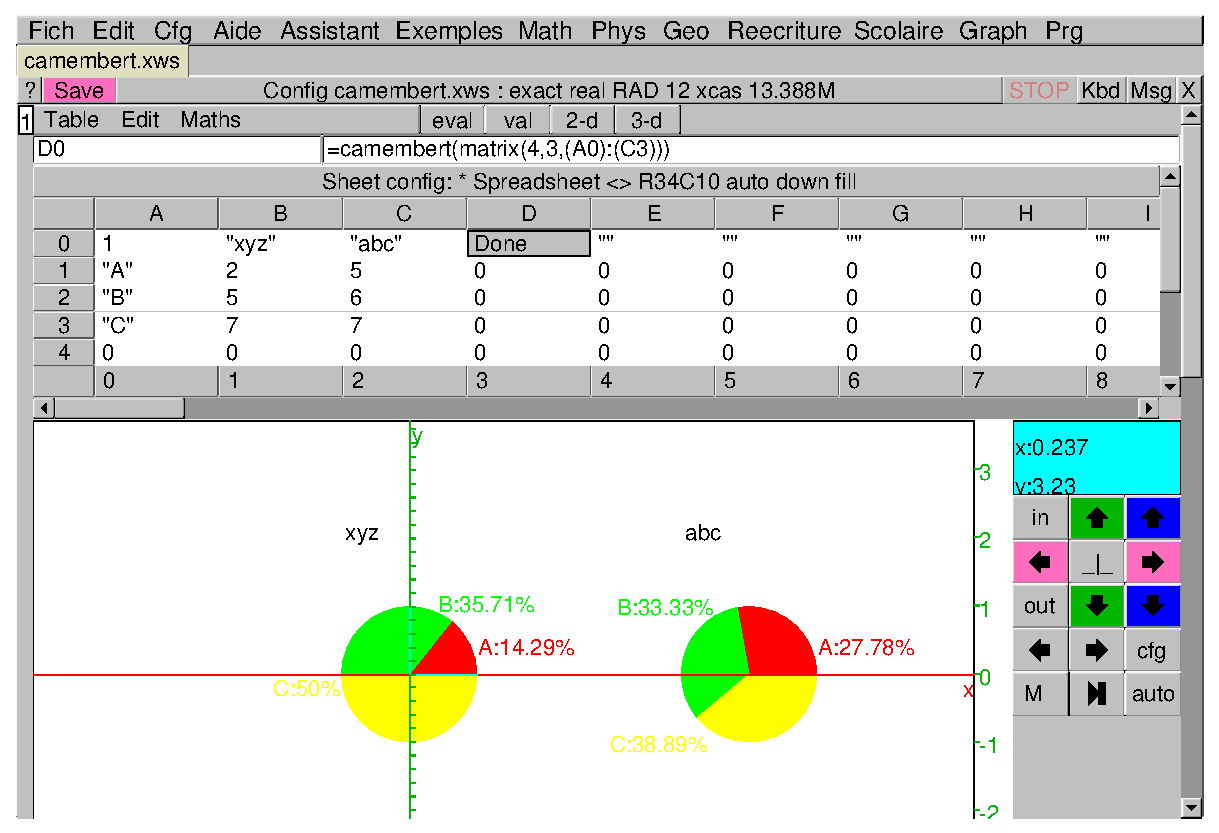
\includegraphics[width=\textwidth]{camemberts}}\end{center}
\item {\tt batons}\\
On peut faire plusieurs diagrammes en batons sur le m\^eme graphique en 
s\'electionnant toute une plage.\\
 {\bf Exemple pour faire deux diagrammes en batons}\\
Avec l'exemple ci-dessus, on met dans {\tt D0} : 
{\tt =diagramme\_batons(matrix(4,3,(A0):(C3)))} \`a l'aide 
du menu {\tt Math$\blacktriangleright$Proba\_stats$\blacktriangleright$1-d$\blacktriangleright$batons}.\\
On obtient :
\begin{center}\framebox{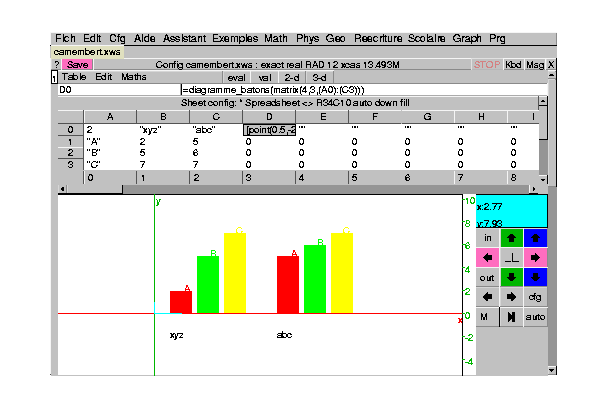
\includegraphics[width=\textwidth]{batons}}\end{center}

\item {\tt plotlist}\\
Si {\tt plotlist} a comme argument une liste {\tt L=[y1,...,yn]}, cela trace 
la ligne reliant les points d'abscisse {\tt 1,...,n} et d'ordonn\'ee 
{\tt L=[y1,...,yn]} et si {\tt plotlist} a comme argument une matrice 
{\tt M=[[x1,y1],...,[xn,yn]]}, cela trace la ligne reliant les points de 
coordonn\'ees {\tt xn,yn}.\\
{\bf Exemple}
On met dans {\tt A} : {\tt 1,2,5,7,9} et dans {\tt B} : {\tt 3,5,6,9,4}
On tape dans {\tt C0} : {\tt =plotlist((A0):(B4),'affichage'=1)}\\
On tape dans {\tt C1} ou  on utilise le menu 
{\tt Math$\blacktriangleright$Proba\_stats$\blacktriangleright$1-d$\blacktriangleright$plotlist} avec pour plage {\tt A0:B4} et pour cellule cible {\tt C1} : 
{\tt =plotlist(matrix(5,2,(A0):(B4)))}\\
{\bf Attention !}
Lorsqu'on met {\tt =plotlist((A0):(B4))} la plage {\tt (A0):(B4)} est applatie 
en une liste (ici la liste {\tt 1,3,2,5,4,6,7,9,9,4})
On obtient en rouge la ligne correspondant \`a la liste et en noir celle
correspondant \`a la matrice :
\begin{center}\framebox{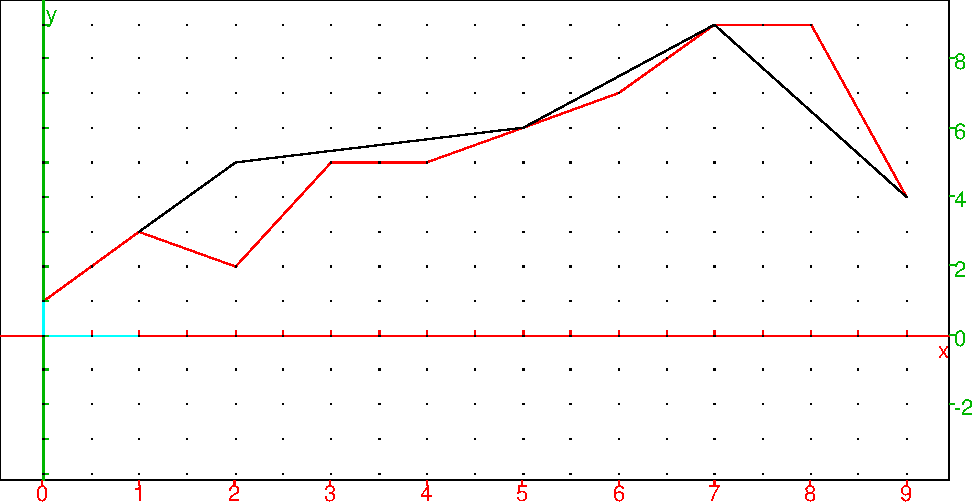
\includegraphics[width=\textwidth]{plotlists}}\end{center}

\item {\tt Boite \`a moustaches} (en anglais {\tt Boxwhiskers})\index{moustache}\index{boxwhisker}\\
{\tt Boite \`a moustaches} permet de dessiner, dans 
l'\'ecran graphique associ\'e au tableur, les 
boites \`a moustaches des colonnes (ou des lignes si {\tt Lignes} est 
coch\'ee) des donn\'ees qui ont \'et\'e s\'electionn\'ees. C'est dans la 
cellule cible  que s'inscrit la commande {\tt moustache} avec comme argument
les valeurs ou les r\'ef\'erences de la plage s\'electionn\'ee  selon que 
l'on coche ou non {\tt valeur}.

\item {\tt Classes (donnees ou donnees/eff)}\\
{\tt Classes}  permet de d\'efinir des classes : on s\'electionne une 
colonne du tableur contenant la s\'erie que l'on veut regrouper en classes (ou 
si on a des effectifs, on s\'electionne deux colonnes du tableur representant 
les donn\'ees et leurs effectifs) puis, on s\'electionne {\tt Classes} dans le 
menu {\tt Statistiques} sous-menu {\tt 1-d} : il faut v\'erifier la valeur 
minimum de la classe, la largeur des classes (ces deux cases sont d\'ej\`a 
remplies avec les valeurs sp\'ecifi\'ees dans la configuration du graphique 
(bouton rouge {\tt geo}) et aussi la cellule cible qui est la 
premi\`ere cellule \`a partir de laquelle on \'ecrira les classes sur deux 
colonnes,
Les intervalles des classes s'inscrivent dans la colonne de la cellule cible 
et commencent par {\tt classe\_min} et la longueur des
 intervalles est \'egale \`a {\tt classe\_size} : ces valeurs peuvent \^etre  
sp\'ecifi\'ees dans la configuration du graphique (bouton rouge {\tt geo}). 
La colonne suivante contient les effectifs des classes obtenues dans la  
pr\'ec\'edente colonne,
\item {\tt Histogramme (intervalles/eff)} (en anglais {\tt Histogram})\\
{\tt Histogramme} permet de dessiner dans l'\'ecran 
graphique associ\'e au tableur l'histogramme de deux colonnes s\'electionn\'ees
representant les intervalles de donn\'ees et leurs effectifs, et
inscrit la commande {\tt histogram} correspondante dans la cellule cible.
\end{itemize}
\subsubsection{Le menu {\tt Maths$\blacktriangleright$stats 2-d} d'un tableur}
Le menu {\tt Maths$\blacktriangleright$stats 2-d} contient les items suivants :
\begin{itemize}
\item {\tt Scatterplot} permet de tracer sur l'\'ecran graphique les points 
d'abscisse la premi\`ere colonne s\'electionn\'ee et d'ordonn\'ee les autres 
colonnes s\'electionn\'ees si {\tt lignes} n'est pas coch\'e ou de tracer sur 
l'\'ecran graphique les points d'abscisse la premi\`ere ligne s\'electionn\'ee 
et d'ordonn\'ee les autres lignes s\'electionn\'ees si {\tt lignes} est 
coch\'e. Les couleurs seront diff\'erentes pour les points
dont les ordonn\'ees sont dans des colonnes (resp lignes) diff\'erentes.\\
Par exemple,
\begin{itemize}
\item  si {\tt lines} n'est pas coch\'e, on remplit :\\
{\tt A0,A1,A2,A3} avec {\tt 1,2,3,4} et \\
{\tt B0,B1,B2,B3} avec {\tt 1,4,9,16}, puis \\
on s\'electionne la matrice {\tt A0:B3} et on ouvre le menu 
{\tt Statistiques 2-d  Scatterplot}.
\item  si {\tt lines} est coch\'e, on remplit :\\
{\tt A0,B0,C0,D0} avec {\tt 1,2,3,4} et \\
{\tt A1,B1,C1,D1} avec {\tt 1,4,9,16}, puis \\
on s\'electionne la matrice {\tt A0:D1} et on ouvre le menu 
{\tt Statistiques 2-d  Scatterplot}.
\end{itemize}
Une boite de dialogue s'ouvre o\`u la plage s\'electionn\'ee est marqu\'ee 
(si vous n'avez rien s\'electionn\'e il faut remplir cette case) puis,
il faut donner le nom de la {\tt cellule cible} l\`a o\`u la commande 
{\tt scatterplot} va s'inscrire. Les valeurs ou les r\'ef\'erences de la plage 
s\'electionn\'ee seront en argument de la commande {\tt scatterplot} selon que 
l'on coche ou non {\tt valeur}.\\
Supposons que {\tt lignes} n'est pas coch\'e.
\begin{itemize}
\item Si {\tt valeur} n'est pas coch\'e dans la boite de dialogue et si la 
cellule cible est {\tt C0}, dans la ligne de 
commande du tableur et dans {\tt C0} il s'inscrit alors :\\
{\tt =scatterplot(matrix(4,2,(A0):(B3)))}
\item Si {\tt valeur} est coch\'e dans la
boite de dialogue et si la cellule cible est {\tt C1}, dans la ligne de 
commande du tableur et dans {\tt C1} il s'inscrit alors :\\
{\tt =scatterplot([[1,1],[2,4],[3,9],[4,16]])}.
\end{itemize}
 Ainsi une modification des 
valeurs de  {\tt A0:B3} modifira, lors d'une r\'e\'evaluation du tableur,le 
graphique command\'e par la case {\tt C0} 
mais ne modifira pas le graphique command\'e par la case {\tt C1}. Autrement 
dit, si vous ne travaillez pas en valeur, c'est \`a dire avec des 
r\'ef\'erences, \`a chaque modification, on aura
une modification du graphique et si vous travailler en valeur \`a chaque 
modification il faudra inscrire dans une nouvelle cellule cible la commande 
{\tt scatterplot} et on aura alors plusieurs graphiques correspondant chacun 
aux commandes {\tt scatterplot} des cellules cibles.\\
{\tt Attention}\\
Lorsqu'on s\'electionne une plage avec la souris on ne peut s\'electionner que 
des colonnes contig\"{u}es. On peut n\'eanmoins remplir la plage de s\'election
de la boite de dialogue avec des colonnes non contig\"{u}es par exemple :\\
{\tt C0..5,A,D} pour dire, si {\tt lines} n'est pas coch\'e, que les points que
l'on veut repr\'esenter ont pour abscisses la colonnes {\tt C} et pour 
ordonn\'ees la colonne {\tt A} d'une part et pour abscisses la colonnes {\tt C}
et pour ordonn\'ees la colonne {\tt D} d'autre part.
Mais dans ce cas {\tt scatterplot} s'affichera comme si 
{\tt valeur} etait coch\'e (m\^eme si ce n'est pas le cas). 

\item {\tt Polygonplot} permet de tracer sur l'\'ecran graphique les points 
d'abscisse la premi\`ere colonne s\'electionn\'ee et d'ordonn\'ee les autres 
colonnes s\'electionn\'ees, en reliant entre eux les points dont les 
ordonn\'ees sont dans une m\^eme colonne.\\
La m\^eme  boite de dialogue que pour {\tt scatterplot} s'ouvre. Dans la ligne
 de commande du tableur il s'inscrit alors, par exemple, dans {\tt D5} :\\
{\tt =polygonplot(matrix(3,3,A0:C2))} si ni {\tt lignes} ni {\tt valeur} ne 
sont coch\'es, si la cellule cible est {\tt D5} et si la plage selectionn\'ee
est {\tt A0:C2}.
\end{itemize}



\section{Pour remplir le tableur}
\subsection{Comment remplir une cellule}
Dans une cellule on peut mettre :\\
\begin{itemize}
\item une chaine de caract\`ere, ou une expression
num\'erique ou formelle : pour cela il suffit de s\'electionner la cellule 
\`a remplir et de taper dans la ligne de commande ce que l'on veut mettre 
dans la cellule, puis de valider avec {\tt enter},
\item une formule faisant r\'ef\'erence aux autres cellules, dans ce cas il 
faut faire pr\'ec\'eder la formule du signe {\tt =} (voir la section 
\ref{sec:references} r\'ef\'erences absolues et relatives).\\
{\bf Attention}\\
1/ Si le curseur ne se trouve pas dans la ligne de commande, lorsqu'on clique 
sur une cellule, la ligne de commande s'efface et le contenu de la cellule
(valeur ou formule) s'affiche dans la ligne de commande.\\
2/ Si le curseur se trouve dans la ligne de commande, il faut que  
la ligne de commande soit vide, pour que, lorsqu'on clique sur une cellule
son contenu s'affiche dans la ligne de commande.\\
3/ Si le curseur se trouve dans la ligne de commande, et que celle-ci contient
quelque chose (par exemple {\tt =}), alors lorsqu'on clique sur une cellule
 c'est son nom qui  s'affiche dans la ligne de commande (ce qui facilite
l'\'edition d'une formule).\\ 
4/ On enl\`eve le curseur de la ligne de commande avec {\tt Esc} ou {\tt Echap}.\\
Ainsi, si la ligne de commande est vide et si, par exemple, on clique sur 
{\tt A1} (qui contient {\tt 3}) alors le contenu de {\tt A1} ({\tt 3}) 
s'affiche dans la ligne de commande : \\
- on peut cliquer dans une autre cellule et alors ligne de commande s'efface 
et son contenu s'affiche dans la ligne de commande.\\
- on peut cliquer dans la ligne de commande, taper quelque chose (par exemple 
{\tt +}), puis cliquer sur une autre  cellule (par exemple {\tt A2}) et alors 
le nom de la cellule {\tt A2} apparait\`a la suite du contenu pr\'ec\'edent 
({\tt 3+}).\\
Donc quand on \'edite le contenu d'une case, si on clique dans le tableur
alors, le nom ou la plage des noms selectionn\'es, s'affichent dans la
ligne de commande.\\
{\bf Exemple}\\
On veut remplir la case {\tt A1} avec la formule {\tt 1+A2} :\\
- on efface la ligne de commande,\\
- on clique sur {\tt A1},\\
- on clique sur la ligne de commande et on tape {\tt =1+},\\
- on clique sur la cellule {\tt A0} puis, {\tt Enter}.\\
Cela marque {\tt 1+A0} dans la cellule {\tt A1}. \\
Pour annuler une modification en  mode \'edition, il n'est donc pas possible de
 simplement cliquer sur une autre cellule du tableur puisque cela recopierait 
le nom de cette autre cellule.
En ligne de commande, c'est la touche {\tt Esc} qui annule l'\'edition.
\item  une liste ou une matrice \`a condition de faire pr\'ec\'eder la liste ou la matrice du signe {\tt =} car, si on ne met pas le signe {\tt =} cela aura pour effet de remplir plusieurs cellules (voir ci-dessous).\\
On peut remplir d'un seul coup plusieurs cellules \`a partie d'une cellule
lorsque l'on met dans cette cellule une liste ou une matrice.\\
Par exemple :\\
Dans {\tt A0} on met : {\tt [1,2,3]}, cela a pour effet de remplir 
{\tt A0} avec {\tt 1}, {\tt B0} avec {\tt 2} et {\tt C0} avec {\tt 3}.\\
Dans {\tt A0} on met : {\tt [[1,2],[3,4]]}, cela a pour effet de
 remplir {\tt A0} avec {\tt 1}, {\tt B0} avec {\tt 2}, {\tt A1} avec {\tt 3} 
et {\tt B1} avec {\tt 4}.\\
{\bf Attention} \\
Le remplissage de plusieurs cellules \`a l'aide d'une matrice ou d'une liste 
n'est possible qu'en \'evaluation directe sans d\'ependance.
Par exemple :\\
On ne peut pas mettre {\tt [A0,B0]} dans {\tt C0}, mais on peut mettre 
{\tt  =[A0,B0]} dans {\tt C0}.
Le signe {\tt =} est necessaire pour remplir {\bf une seule} cellule avec
 une liste ou une matrice.\\
{\bf Exemple}\\
 Pour mettre une liste ou une matrice dans une case il 
faut mettre le signe {\tt =} devant la liste ou la matrice.\\ 
On tape dans la case {\tt A0} :\\
{\tt =[[1,2],[3,4]]}\\
On obtient dans la case {\tt A0} :\\
{\tt [[1,2],[3,4]]}\\
Si l'on ne met pas le signe \'egal on peut remplir d'un seul coup plusieurs 
cases du tableur par les \'el\'ements de la liste ou de la matrice  \`a 
condition que la formule mise ne fasse pas r\'ef\'erence aux autres cellules.\\
On tape dans la case {\tt A0}:\\
{\tt [[1,2],[3,4]]}\\
On obtient :\\
{\tt A0=1}, {\tt B0=2}, {\tt A1=3}, {\tt B1=4}\\
{\bf Autre exemple}\\
Dans {\tt A0} je tape :\\
{\tt ranm(2,3,4)}\\
Je remplis alors d'un seul coup les 6 cases : {\tt A0,B0,C0,A1,B1,C1} avec  
les \'el\'ements de la matrice {\tt [[1,3,1],[2,1,2]]} (en effet 
{\tt ranm(2,3,4)} renvoie une matrice de 2 lignes et 3 colonnes 
d'entiers pris au hasard de fa\c{c}on \'equir\'epartie dans l'ensemble des 4 
nombres {\tt 0,1,2,3}.\\
Cette matrice est d\'efinie une fois pour toute car la formule 
{\tt ranm(2,3,4)} est \'evalu\'ee puis oubli\'ee.\\
Dans {\tt A0} je tape :\\
{\tt =ranm(2,3,4)}\\
Cette fois, seule la cellule {\tt A0} est remplie avec la matrice :\\
{\tt [[1,2,3],[3,2,2]]}.\\
Cette matrice changera \`a chaque modification du tableur sauf, si on a 
choisi {\tt Ne pas recalculer automatiquement} dans la configuration du tableur
(avec le menu {\tt Edit$\blacktriangleright$Configuration}).
\end{itemize}
\subsection{Pour voir le contenu d'une cellule}
Lorsqu'on consulte le tableur, toutes les cellules sont \'evalu\'ees. 
Pour voir le contenu \'evalu\'e d'une cellule situ\'ee hors du champ de vision,
on utilise, soit le curseur vertical (situ\'e \`a droite du tableur) qui permet
 de voir les derni\`eres lignes, soit le curseur horizontal (situ\'e \`a la 
derni\`ere ligne du tableur) qui permet de voir les derni\`eres colonnes.\\
{\bf Remarque}\\
Lorsque toutes les cellules sont visibles, ces deux curseurs ne sont pas 
pr\'esents. \\
Pour voir le contenu non \'evalu\'e d'une cellule (c'est \`a dire ce que l'on 
a mis, initialement, dans la cellule comme formule ou comme valeur), 
il suffit de cliquer sur 
cette cellule : il apparait alors dans la ligne de commande la formule (ou 
la valeur) qui a \'et\'e mise dans cette cellule.\\
Pour faire apparaitre dans la ligne de commande, le contenu \'evalu\'e de 
la cellule, il suffit d'appuyer sur le bouton {\tt eval}.\\
Lorsque le r\'esultat est trop grand (ou trop petit) en taille on peut avoir 
besoin d'agrandir une colonne pour voir ce r\'esultat enti\`erement (ou de 
diminuer la colonne pour gagner de la place). Par exemple, on veut modifier 
la taille de la colonne {\tt B},  on 
d\'eplace la souris sur le trait vertical qui s\'epare {\tt B} de {\tt C} : 
le curseur devient $\leftrightarrow$. On clique avec la souris et, sans 
relacher le bouton de la souris, on d\'eplace ce trait vertical pour agrandir 
ou diminuer la largeur de la colonne {\tt B}.
Lorsque le r\'esultat est trop grand, on peut aussi appuyer sur le bouton 
{\tt eval} pour faire apparaitre ce r\'esultat dans la ligne de commande.
%fin de a faire
\subsection{R\'ef\'erences absolues et relatives}\label{sec:references}
Dans une cellule on peut mettre :\\
- une chaine de caract\`eres,\\
- une expression alg\'ebrique,\\
- une formule faisant r\'ef\'erence \`a d'autres cellules. Ces r\'ef\'erences
peuvent \^etre absolues ou relatives \`a la cellule qui contient la formule. 
Les r\'ef\'erences absolues sont obtenues en rajoutant {\tt \$} devant la 
lettre d\'esignant la colonne ou devant le num\'ero de la ligne de la cellule 
r\'ef\'erence.\\
Les r\'ef\'erences relatives permettent de d\'esigner les cellules par 
rapport \`a une autre : ainsi  {\tt A0} mis dans la cellule {\tt B1} d\'esigne 
la cellule situ\'ee dans la colonne pr\'ec\'edente et \`a la ligne 
pr\'ec\'edente et c'est cette information qui sera recopi\'ee quand on
 recopiera la formule vers le bas ou vers la droite.\\
Exemples :\\
Dans {\tt A0} il y a 1 et je tape dans {\tt B1} la formule :
\begin{itemize}
\item {\tt \$A\$0+2} : dans {\tt B1} il y aura 3, et si je recopie cette 
formule vers le bas, j'obtiens  des 3 dans la colonne {\tt B} car je recopie 
dans toutes les cases de la colonne {\tt B} la formule {\tt \$A\$0+2}. Si je 
recopie cette formule vers la droite, j'obtiens  aussi des 3 dans la 
premi\`ere ligne, car je recopie dans toutes les cases de la premi\`ere ligne 
la formule {\tt \$A\$0+2} puisque {\tt \$A\$0} est la r\'ef\'erence absolue 
de la case {\tt A0}.
\item {\tt \$A0+2} : dans {\tt B1} il y aura 3, et si je recopie cette formule 
vers le bas cette formule deviendra {\tt \$A1+2} dans {\tt B2}, {\tt \$A2+2} 
dans {\tt B3}. La valeur de {\tt B2} d\'epend donc de la valeur de {\tt A1}, 
la valeur de {\tt B3} d\'epend donc de la valeur de {\tt A2} etc...\\ 
Si je recopie cette formule vers la droite, cette formule deviendra 
{\tt \$A0+2} dans {\tt C1}, {\tt \$A0+2} dans {\tt D1} ...j'obtiens  
donc une ligne de 3. {\tt \$A0} fait toujours r\'ef\'erence \`a la colonne 
{\tt A} : {\tt A} est une r\'ef\'erence absolue mais {\tt 0} d\'esigne ici la 
ligne pr\'ec\'edente puisque {\tt \$A0} a \'et\'e mis dans {\tt B1}. 
\item  {\tt A\$0+2} : dans {\tt B1} il y aura 3, et si je recopie cette formule
vers le bas, j'obtiens des 3 dans la colonne {\tt B} mais si je recopie cette 
formule vers la droite, cette formule deviendra {\tt B\$0+2} dans {\tt C1}, 
{\tt C\$0+2} dans {\tt D1} etc... 
\item {\tt A0+2} : dans {\tt B1} il y aura 3, et si je recopie cette formule 
vers le bas, cette formule deviendra {\tt A1+2} dans {\tt B2}, {\tt A2+2} dans 
{\tt B3} etc...si je recopie cette formule vers la droite, cette formule 
deviendra {\tt B0+1} dans {\tt C1}, {\tt C0+1} dans {\tt D1} etc... 
\end{itemize}
\subsection{R\'ef\'erence d'un sous-tableau}
Il y a deux fa\c{c}ons de d\'esigner un morceau du tableur selon que l'on veut 
remplir une cellule ou le s\'electionner dans la {\tt case de s\'election}.\\
 Il sera d\'esign\'e par :
\begin{itemize}
\item dans une cellule, par la r\'ef\'erence de sa premi\`ere case puis 
"deux points" ({\tt :}), puis la r\'ef\'erence de sa derni\`ere case.\\
Les r\'ef\'erences de la premi\`ere ou de la derni\`ere case seront selon les 
cas, absolues ou relatives, mais {\bf attention} cela est valable pour des 
colonnes contig\"ues et repr\'esente une liste i.e. le tableau est aplati,
\item dans la {\tt case de s\'election} par
r\'ef\'erence de sa premi\`ere case puis "point point" ({\tt ..}), puis le
num\'ero de la derni\`ere ligne, puis virgule ({\tt ,}) suivi de la s\'equence 
des lettres d\'esignant les colonnes. Cette fois cela repr\'esente une matrice
est on peut facilement d\'esigner des colonnes non contig\"ues.
\end{itemize}
{\bf Remarque}
Dans la {\tt case de s\'election}, on ne peut pas utiliser "deux points" 
({\tt :}) comme s\'eparateur entre les deux r\'ef\'erences.\\
{\bf Exemple}\\
Dans une cellule  {\tt A0:B5} repr\'esente la liste des valeurs de
{\tt [A0,B0,A1,B1,..,A5,B5]} constitu\'ee par la matrice "aplatie".\\
Dans la {\tt case de s\'election}, {\tt A0..B5} d\'esigne le tableau de 6 
lignes (lignes 0,1..5) et 2 colonnes (colonnes {\tt A} et {\tt B}).\\
On a aussi la possibilit\'e de d\'esigner dans la 
{\tt case de s\'election} des colonnes non cons\'ecutives, on \'ecrira par 
exemple {\tt A0..10,C,E} pour s\'electionner 
les 11 premi\`eres lignes des colonnes {\tt A}, {\tt C} et {\tt E}.\\
{\bf Attention!!!} \\
Seule la {\tt case de s\'election} permet de d\'efinir un 
sous-tableau ou une matrice.\\  
Donc dans une cellule pour d\'esigner un sous-tableau on peut reconstituer la 
matrice \`a l'aide de la commande {\tt list2mat} (qui transforme une liste en 
matrice selon le nombre de colonnes sp\'ecifi\'e) si les colonnes sont 
cons\'ecutives ou en utilisant la commande 
{\tt tran} (qui transforme une matrice en sa transpos\'ee).\\
Dans la  cellule {\tt F0} on tape par exemple :\\
 {\tt =list2mat(A0:B5,2)} pour avoir une matrice avec 2 colonnes et 6 lignes
Dans la  cellule {\tt F0} on tape par exemple :\\
{\tt =list2mat(A0:D5,4)} pour avoir une matrice avec 4 colonnes et 6 
lignes dans la  cellule {\tt F0}.\\
Dans la  cellule {\tt F0} on tape par exemple :\\
 {\tt =tran([A0:A3,C0:C3])} pour avoir une matrice avec 2 colonnes et 4
lignes dans la  cellule {\tt F0}.\\
Dans la  cellule {\tt F0} on tape par exemple :\\
 {\tt =tran([A0:A3,B0:B3,C0:C3])} pour avoir une matrice avec 3 colonnes et 4
lignes dans la  cellule {\tt F0}.\\
{\bf Attention!!!} \\
On ne peut pas remplir plusieurs cellules d'un seul coup avec une matrice
contenant des r\'ef\'erences \`a d'autres cellules : quand il y a une formule
 faisant des r\'ef\'erences \`a d'autres cellules on ne peut remplir qu'une 
seule cellule et il faut mettre le signe {\tt =} devant la formule.
\section{Pour sauver l'\'ecran du tableur}
\subsection{Pour sauver une matrice}
Vous avez rempli l'\'ecran du tableur avec une matrice.

Pour sauver cette matrice vous pouvez utiliser le bouton {\tt Save} de la barre
de boutons cela sauvera la matrice sous le nom inscrit dans la ligne d'\'etat 
apr\`es {\tt Spreadsheet} (en g\'en\'eral le m\^eme nom que le nom du fichier 
sans son extension {\tt .tab} ou vous pouvez utiliser le menu {\tt Fich} 
sous-menu {\tt Nom de variable} en donnant un autre nom de variable.

Pour sauver une sous-matrice, il faut la s\'electionner soit avec la souris, 
soit en utilisant la case de s\'election et ensuite 
utiliser le menu {\tt Fich} sous-menu  {\tt Sauver selection vers variable} 
puis donner le nom de la variable qui stockera la matrice s\'electionn\'ee 
(cf \ref{sec:sauver}).\\
La format est celui d'une matrice. On aura donc dans la variable design\'ee
 une matrice par exemple : {\tt [[1,2,3,4,5],[1,0,2,0,1],[...]]}
\subsection{Pour sauver un tableur}\label{sec:sauve}
Vous avez rempli un tableur avec diff\'erentes formules. Pour sauver ce 
tableur il suffit d'utiliser le bouton {\tt sauver} de la barre de boutons ou 
on utilise le menu {\tt Fich} sous-menu {\tt Sauver comme} (cf \ref{sec:sauver}).\\
Lorsque vous sauvez ainsi, vous sauvez \`a la fois les formules et les valeurs.
En effet, le format de sauvetage est une matrice dont chaque coefficient est 
une liste de trois \'el\'ements : le premier \'el\'ement est la formule qui 
d\'efinit la cellule, le deuxi\`eme \'el\'ement est la valeur prise par la 
cellule et le troisi\`eme est une variable d\'etat interne.\\
On aura par exemple {\tt spreadsheet[[[3,3,2],[=A0+1,4,2]],[...]]},
cela vaut dire que {\tt A0=3}, que {\tt B0=A0+1} et que la valeur de 
{\tt B0} est {\tt 4}.\\
Lors d'une \'evaluation du tableur, la troisi\`eme  valeur vaut :\\ 
{\tt 0} si la cellule n'a pas encore \'et\'e recalcul\'ee,
{\tt 1} si la cellule est en cours de calcul,\\
 {\tt 2} si la cellule a \'et\'e calcul\'ee.

L'algorithme est le suivant :\\
1/ On fait toutes les cellules de la gauche vers la droite
et du haut vers le bas,\\
2/ Si le troisi\`eme argument de la cellule vaut 2, c'est fini.
Si le troisi\`eme argument de la cellule vaut 1, on envoie une erreur :
"\'evaluation r\'ecursive", \\
3/ le troisi\`eme argument de la cellule vaut 0, on le met \`a 1 et
on cherche toutes les cellules d\'ependant de cette cellule,
on calcule leurs valeurs et on remplace puis, on met \`a  2 le troisi\`eme 
argument de la cellule.
\section{Pour copier une partie du tableur dans une ligne d'enr\'ee}
\subsection{Pour copier une seule cellule du tableur dans une ligne d'enr\'ee}
Il faut s\'electionner la cellule \`a recopier avec la 
souris et se servir du bouton {\tt copier} du tableur.\\
Puis, on met le curseur dans une ligne d'enr\'ee, puis on appuie sur la touche 
{\tt coller}, et la cellule  est recopi\'ee dans la ligne de commande.
\subsection{Pour copier plusieurs cellules du tableur dans une ligne d'entr\'ee}
Si les cellules sont cons\'ecutives, on peut les s\'electionner avec la 
souris, sinon on utilisera la {\tt case de s\'election}.\\
On tape par exemple dans la {\tt case de s\'election} :\\
{\tt A0..3,D}\\
les quatre premi\`eres cellules des colonnes {\tt A} et {\tt D} sont alors 
s\'electionn\'ees.\\
Puis, on met le curseur dans une ligne de commande et on appuie sur la touche 
{\tt coller}, et les quatre 
premi\`eres cellules des colonnes {\tt A} et {\tt D} sont recopi\'ees dans la
ligne de commande.

\section{Les fonctions sp\'ecifiques du tableur}
\subsection{Tableau de valeurs de  $f(x)$ : {\tt tablefunc}}\index{tablefunc}\label{sec:tablefunc}
On peut avoir, dans le tableur, le tableau des valeurs num\'eriques d'une 
expression $f(x)$ pour $x=x0,\ x0+h,\ x0+2*h....$ en tapant dans la ligne 
de commande du tableur :\\
{\tt tablefunc(f(x),x,x0,h)} ou  {\tt tablefunc(f(x),x)}.\\
Apr\`es avoir selectionn\'e {\tt A0}, on tape, par exemple, dans la ligne de 
commande du tableur :\\
\begin{center}{\tt tablefunc(x\verb|^|2,x,-1,0.2)}\end{center}
On obtient si on a 15 lignes :\\
\begin{center}{\tt \begin{tabular}{|l|l|l|}
\hline
 &A&B\\
\hline
0 & $x$ &$x^2$\\
\hline
1 &0.2.0&"Tablefunc"\\
\hline
2& -1&1.0\\
\hline
3 & -0.8 & 0.64\\
\hline
4 & -0.6 &0.36\\
\hline
.. &..&..\\
\hline
14 &1.4 &1.96\\
\hline
\end{tabular}}\end{center}
Dans le cas o\`u les valeurs du point de d\'epart {\tt x0} et du pas {\tt h} ne
sont pas pr\'ecis\'ees, ces valeurs valent par d\'efaut {\tt x0=X-} et 
{\tt h=((X+)-(X-))/10} o\`u {\tt X-} et {\tt X+} sont d\'efinis dans la 
configuration du graphique (bouton rouge {\tt geo}) et valent au d\'emarrage
{\tt X-=-5.0} et {\tt X+=5.0} et donc  {\tt x0=-5.0} et {\tt h=1.0}.\\

On peut donc avoir aussi dans le tableur, les valeurs  num\'eriques des termes
 d'une suite $u_n=f(n)$ pour $n=n0,\ n0+1,\ n0+2,....$ en tapant dans la 
ligne de commande du tableur :\\
{\tt tablefunc(f(n),n,n0)}.\\
Apr\`es avoir selectionn\'e {\tt A0}, on tape, par exemple, dans la ligne de 
commande du tableur :\\
\begin{center}{\tt tablefunc(n\verb|^|2,n,5,1)}\end{center}
On obtient si on a 15 lignes :\\
\begin{center}{\tt \begin{tabular}{|l|l|l|}
\hline
 &A&B\\
\hline
0 & $n$ &$n^2$\\
\hline
1 &1.0&"Tablefunc"\\
\hline
2& 5&25.0\\
\\\hline
3 & 6.0 & 36.0\\
\hline
4 & 7.0 &49.0\\
\hline
.. &..&..\\
\hline
14 &17.0 &289.0\\
\hline
\end{tabular}}\end{center}
{\bf Remarque}\\
 Lorsque la colonne {\tt A} est s\'electionn\'ee, {\tt tablefunc(f(x),x,x0,h)}
 a pour effet de placer, dans la colonne {\tt A} et \`a partir de la ligne 
{\tt 0} :\\ {\tt x,h,x0,A2+A\$1} et,\\
dans la colonne {\tt B} et \`a partir de la ligne {\tt 0} :\\ 
{\tt f(x),"Tablefunc",evalf(subst(B\$0,A\$0,A2))}
\subsection{Termes d'une suite r\'ecurrente : {\tt tableseq}}\index{tableseq}\label{sec:tableseq}
On peut avoir, dans le tableur, les valeurs num\'eriques des termes d'une suite
 r\'ecurrente (${\tt u_0=u0, \ u_n=f(u_{n-1})}$) gr\^ace \`a la commande :\\ 
{\tt tableseq(f(n),n,u0)}.\\
Apr\`es avoir selectionn\'e {\tt A0}, on tape, par exemple, dans la ligne de 
commande du tableur :
\begin{center}{\tt tableseq(0.5*(n+3/n),n,3)}\end{center}
On obtient, si on a 7 lignes :
\begin{center}{\tt \begin{tabular}{|l|l|}
\hline
 &A\\
\hline
0 & 0.5*(n+3/n)\\
\hline
1 & n\\
\hline
2 & 3\\
\hline
3 & 2\\
\hline
4 & 1.75\\
\hline
.. &..\\
\hline
7 &1.73205080757\\
\hline
\end{tabular}}\end{center}
Apr\`es avoir selectionn\'e {\tt B0}, on tape, par exemple, dans la ligne de 
commande du tableur :
\begin{center}{\tt tableseq(x+y,[x,y],[1,1])}\end{center}
On obtient, les premiers termes de la suite de Fibonacci :
\begin{center}{\tt \begin{tabular}{|l|l|}
\hline
 &B\\
\hline
x+y & \\
\hline
1 & x\\
\hline
2 & y\\
\hline
3 & 1\\
\hline
4 & 1\\
\hline
5 & 2\\
\hline
.. &..\\
\hline
7 & 5\\
\hline
.. &..\\
\hline
\end{tabular}}\end{center}
{\bf Remarque}\\
 Lorsque la colonne {\tt E} est s\'electionn\'ee, 
{\tt tableseq(f(n),n,u0)} a pour effet de placer,
dans la colonne {\tt E} et \`a partir de la ligne {\tt 0} :\\ 
{\tt f(n),n,u0,evalf(subst(E\$0,E\$1,E2))}.
\section{R\'ef\'erences de la cellule active : {\tt Row} et {\tt Col}}\index{Row}\index{Col}
{\tt Row} et {\tt Col} sont des fonctions qui sont utilisables essentiellement
dans le tableur, en dehors du tableur {\tt Row} et {\tt Col} sont le num\'ero 
de la ligne et de la colonne de la cellule s\'electionn\'ee du dernier tableur
\'evalu\'e.\\
\noindent {\tt Row} n'a pas des param\`etre et renvoie le num\'ero de la ligne 
de la cellule courrante.\\
On tape quand la cellule {\tt C4} est mise en surbrillance :\\
{\tt Row()}\\
On obtient :\\
{\tt 4}\\
{\tt Col} n'a pas des param\`etre et renvoie le num\'ero de la colonne 
de la cellule courrante (la colonne {\tt A} a pour num\'ero 0, 
la colonne {\tt B} a pour num\'ero 1 etc...)\\
On tape quand la cellule {\tt C4} est mise en surbrillance :\\
{\tt Col()}\\
On obtient :\\
{\tt 3}\\
Ainsi si dans la cellule {\tt A0} je mets :\\
{\tt =Row()+Col()}
puis je recopie cette formule vers le bas et j'obtiens :\\
dans la colonne {\tt A} :\\
 {\tt 0,1,2,3,4...}\\
puis je recopie cette formule vers la droite depuis {\tt A0} et j'obtiens :\\
dans la ligne {\tt 0} :\\
 {\tt 0,1,2,3,4...}\\
puis je recopie cette formule vers la droite depuis {\tt A1} et j'obtiens :\\
dans la ligne {\tt 1} : \\
{\tt 1,2,3,4,5...} etc...\\
{\bf Attention} Bien mettre le signe {\tt =} car {\tt Row()} et {\tt Col()}
font r\'ef\'erences \`a la ligne et \`a la colonne de la cellule dans laquelle 
se trouve la formule.
\section{Nommer une cellule par une variable : {\tt current\_sheet}}\index{current\_sheet}\label{sec:currentsheet}
\noindent{\tt current\_sheet} est une fonction qui est utilisable
 essentiellement dans le tableur, en dehors du tableur {\tt current\_sheet}
permet d'avoir acc\`es aux cellules du dernier tableur \'evalu\'e.\\ 
{\tt current\_sheet} s'utilise soit avec :\\
- aucun  param\`etre : {\tt current\_sheet()} renvoie le tableur tout entier,\\
- un param\`etre entier : {\tt current\_sheet(j)} renvoie  la ligne {\tt j} 
du tableur,\\
- deux param\`etres entiers : {\tt current\_sheet(j,k)} renvoie  la cellule du 
tableur situ\'ee \`a  la ligne {\tt j} et \`a la colonne {\tt k}.\\
Ainsi {\tt current\_sheet(3,1)} d\'esigne la cellule {\tt B3}.\\
Cela permet de d\'esigner une cellule par deux variables enti\`eres, 
par exemple :\\
{\tt j:=3;k:=1;current\_sheet(j,k)}\\
{\bf Remarque}\\
Pour avoir la colonne {\tt k} du tableur dans une ligne de commande, il faut 
taper :\\
{\tt tran(current\_sheet())[k]} (puisque {\tt tran(current\_sheet())} 
d\'esigne la transpos\'ee du tableur).\\
On peut bien s\^ur utiliser {\tt current\_sheet} dans le tableur.\\
On tape :\\
{\tt =current\_sheet(1,2)}\\
ou encore, on peut prendre la valeur d'une case comme indice : \\
si {\tt A0} contient 1 et {\tt B1} contient 2 on peut taper,
{\tt =current\_sheet(A0,B1)}.\\
{\bf Exemple d'utilisation} :\\ 
On tape la suite des nombres entiers dans la colonne {\tt A}.\\
On tape dans {\tt A0} :\\
{\tt 1}\\
 puis on tape dans {\tt A1} :\\
{\tt  =A0+1}\\
formule que l'on recopie avec avec le menu 
{\tt Edit} du tableur, puis, {\tt Remplir} et {\tt Copier vers le bas}.\\
Dans la colonne {\tt B} on met, par exemple, la suite  
$u_n=\sum_{k=0}^n(-1)^k/(k+1)$.\\
On tape dans  {\tt B0} :\\ 
{\tt 1}\\
puis on tape dans {\tt B1} :\\
{\tt =B0+(-1)\verb|^|A1/(A1+1)}, formule que l'on recopie avec le menu 
{\tt Edit} du tableur, puis, {\tt Remplir} et {\tt Copier vers le bas}.\\
On veut extraire de cette suite, les termes d'indice pair dans la colonne 
{\tt C}, on tape dans {\tt C0} :\\
{\tt =current\_sheet(2*A0,1)}, formule que l'on recopie 
avec {\tt remplir} et {\tt vers le bas}.\\
On veut extraire de cette suite les termes d'indice impair dans la colonne 
{\tt D}, on tape dans {\tt D0} :\\
 {\tt =current\_sheet(2*A0+1,1)}, formule que l'on recopie avec le menu 
{\tt Edit} du tableur, puis, {\tt Remplir} et {\tt Copier vers le bas}.\\
Ou encore on utilise {\tt Row} et on n'a besoin que de 3 colonnes .\\
On tape dans {\tt A0} :\\
{\tt 1}\\
 puis on tape dans {\tt A1} :\\
{\tt =A0+(-1)\verb|^|Row()/(Row()+1)}, formule que l'on recopie avec le menu 
{\tt Edit} du tableur, puis, {\tt Remplir} et {\tt Copier vers le bas}.\\
On veut extraire de cette suite, les termes d'indice pair dans la colonne 
{\tt B}, on tape dans {\tt B0} :\\
{\tt =current\_sheet(2*Row(),0)}, formule que l'on recopie 
avec {\tt remplir} et {\tt vers le bas}.\\
On veut extraire de cette suite les termes d'indice impair dans la colonne 
{\tt C}, on tape dans {\tt C0} :\\
 {\tt =current\_sheet(2*Row()+1,0)}, formule que l'on recopie avec le menu 
{\tt Edit} du tableur, puis, {\tt Remplir} et {\tt Copier vers le bas}.

\section{Compter les \'el\'ements du tableur v\'erifiant une propri\'et\'e}
 On suppose que dans la colonne {\tt A} il y a {\tt 1,2,3,4}, dans la colonne
{\tt B} il y a {\tt 2,4,6,8} et dans la colonne {\tt C} il y a 
{\tt 4,8,12,16}.\\
{\bf Attention !}\\
Pour d\'esigner une plage du tableur, on tape {\tt A0:C3}, mais {\tt Xcas} le 
raplatit en une liste : dans l'exemple ci-dessus  {\tt A0:C3=[1,2,2,4,3,6]} 
{\bf Remarque}\\
Pour avoir une m\'ethode rapide pour compter, par exemple, les sommes obtenues
lorsqu'on  lance  101 fois deux d\'es. On remplit al\'eatoirement les colonnes
{\tt A} et {\tt B} en tapant  {\tt ranm(101,1)} comme valeur pour {\tt A0} et 
{\tt B0}.
Il faut cr\'eer une cellule tampon, qui contiendra le tableau des
valeurs de la zone \`a analyser. On place simplement dans
cette cellule la definition de la plage pr\'ec\'ed\'ee de =, par exemple
si {\tt A0} \`a {\tt B100} contient des jets de deux d\'es, et que 
{\tt C} contient la somme de la colonne {\tt A} et de la colonne {\tt B},
on met dans {\tt D0} : {\tt = C0:C100}.\\
Ensuite dans {\tt D2} \`a {\tt D12} on ecrit :\\
{\tt =count\_eq(2,D0)}... {\tt count\_eq(12,D0)}\\
Ainsi le calcul de la plage {\tt C0:C100} qui est long n'est fait qu'une
fois. C'est le meme principe qu'en programmation, on utilise une
variable intermediaire (la cellule tampon {\tt D0}).
\subsection{Compter les \'el\'ements d'un sous tableau v\'erifiant une propri\'et\'e : {\tt count}}\index{count}
\noindent{\tt count} a deux ou trois param\`etres : une fonction r\'eelle 
{\tt f} et une liste ou un sous-tableau \'eventuellement un param\`etre 
optionnel {\tt row} ou {\tt col}.\\

{\bf Attention} dans le tableur les param\`etre optionnels {\tt row} ou 
{\tt col} ne servent pas, car dans une ligne du tableur 
un sous-tableau (par exemple {\tt A0:C3}) d\'esigne une liste : en effet
si dans une cellule on met {\tt =A0:C3}, la cellule contient la liste obtenue 
en mettant les lignes du sous tableau {\tt A0:C3} bout \`a bout.\\
Si vous voulez utiliser le sous tableau (par exemple {\tt A0:C3}) comme une 
matrice il faut mettre dans une cellule {\tt =list2mat(A0:C3),3)} (car {\tt 3} 
est le nombre de colonnes de {\tt A0:C3}). On peut aussi sauver la s\'election 
{\tt A0:C3} vers une variable (menu {\tt Table}), car lors de cette affectation
la matrice n'est pas aplati et donc cette variable contient une matrice.\\

{\tt count} applique la fonction aux \'el\'ements de la 
liste ou du sous-tableau et en renvoie la somme.\\
Si {\tt f} est une fonction bool\'enne {\tt count} renvoie le nombre 
d'\'el\'ements de la liste ou du sous-tableau pour lesquels la fonction 
bool\'enne est vraie.\\
On tape dans une cellule :
\begin{center}{\tt =count((x)->x,A0:C3)}\end{center}
On obtient :
\begin{center}{\tt  70}\end{center}
En effet, la somme des \'el\'ements de {\tt A0:C3} vaut {\tt (1+2+3+4)*7=70}
car dans A il y a 1,2,3,4 dans B il y a 2*A soit 2,4,6,8 et dans C il y a 4*A 
soit 4,8,12,16 donc en tout il y a 7*A.\\
On tape dans une cellule :
\begin{center}{\tt =count((x)->(x<10 and x>5),A0:C3)}\end{center}
On obtient :
\begin{center}{\tt  3}\end{center}
En effet, il y a {\tt 6,8,8}, soit 3 \'el\'ements qui sont entre 5 et 10.
\subsection{Compter les \'el\'ements ayant une valeur donn\'ee : {\tt count\_eq}}\index{count\_eq}
\noindent{\tt count\_eq} a deux ou trois param\`etres : une nombre et une liste
r\'eelle ou un sous-tableau et \'eventuellement un param\`etre 
optionnel {\tt row} ou {\tt col}.\\
{\bf Attention} dans le tableur les param\`etre optionnels {\tt row} ou 
{\tt col} ne servent pas, car dans le tableur car un sous-tableau est aplati en
 une liste.\\
{\tt count\_eq} renvoie le nombre d'\'el\'ements de la liste ou du sous-tableau
qui sont \'egaux au premier argument.\\
On tape dans une cellule :
\begin{center}{\tt =count\_eq(4,A0:C3)}\end{center}
On obtient :
\begin{center}{\tt  3}\end{center}
car dans A il y a 1,2,3,4 dans B il y a 2*A soit 2,4,6,8 et dans C il y a 4*A 
soit 4,8,12,16.
\subsection{Compter les \'el\'ements plus petits qu'une valeur donn\'ee : {\tt count\_inf}}\index{count\_inf}
\noindent{\tt count\_inf} a deux ou deux param\`etres : une nombre et une liste
r\'eelle ou un sous-tableau et \'eventuellement un param\`etre 
optionnel {\tt row} ou {\tt col}.\\
{\bf Attention} dans le tableur les param\`etre optionnels {\tt row} ou 
{\tt col} ne servent pas, car dans le tableur car un sous-tableau est aplati en
 une liste.\\
{\tt count\_inf} renvoie le nombre d'\'el\'ements de la liste (ou du 
sous-tableau qui sont strictement inf\'erieurs au premier argument.\\
On tape dans une cellule :
\begin{center}{\tt =count\_inf(4,A0:C3)}\end{center}
On obtient :
\begin{center}{\tt  4}\end{center}
car dans A il y a 1,2,3,4 dans B il y a 2*A soit 2,4,6,8 et dans C il y a 4*A 
soit 4,8,12,16.

\subsection{Compter les \'el\'ements plus grands qu'une valeur donn\'ee : {\tt count\_sup}}\index{count\_sup}
\noindent{\tt count\_sup} a deux ou trois param\`etres : une nombre et une 
liste r\'eelle ou un  sous-tableau et \'eventuellement un param\`etre 
optionnel {\tt row} ou {\tt col}.\\
{\bf Attention} dans le tableur les param\`etre optionnels {\tt row} ou 
{\tt col} ne servent pas, car dans le tableur car un sous-tableau est aplati en
 une liste.\\
{\tt count\_sup} renvoie le nombre d'\'el\'ements de la liste 
ou du sous-tableau qui sont  strictement sup\'erieurs au premier argument.\\
On tape dans une cellule :
\begin{center}{\tt =count\_sup(4,A0:C3)}\end{center}
On obtient :
\begin{center}{\tt  5}\end{center}
car dans A il y a 1,2,3,4 dans B il y a 2*A soit 2,4,6,8 et dans C il y a 4*A 
soit 4,8,12,16.
\section{Les fonctions statistiques \`a une variable du tableur}
\subsection{Les fonctions graphiques}
On peut utiliser directement le graphique depuis le tableur : les fonctions 
graphiques peuvent \^etre utilis\'ees dans une cellule. Pour avoir 
l'histogramme, la boite \`a moustaches, un nuage de points ou une ligne 
polygonale  depuis le tableur on peut se servir du menu {\tt Maths} du
tableur (puis {\tt stats 1-d}) apr\`es avoir s\'electionn\'e dans le 
tableur l'argument avec la souris ou avec la {\tt case de s\'election}.
Dans ce cas, une boite de dialogue s'ouvre, vous devez choisir la cellule cible
(c'est dans cette cellule que s'inscrira la commande graphique), vous pouvez
\'eventuellement modifier la s\'election (en mettant par exemple {\tt A1..B6}
dans {\tt cellules entr\'ee}), vous pouvez cocher (resp ne pas cocher) 
{\tt valeur} pour que la commande graphique ait pour argument les valeurs 
(resp les r\'ef\'erences) de la s\'election : donc si {\tt valeur} n'est pas 
coch\'ee un changement de valeur dans une cellule de la s\'election aura pour 
cons\'equence un changement du graphique, si on est en mode automatique ou si 
on appuie sur le bouton {\tt eval}.\\
Ou encore, on peut taper la commande correspondante (ou se servir du menu 
{\tt Math$\blacktriangleright$Proba\_stats$\blacktriangleright$1-d}) dans la 
ligne de commande du tableur en recopiant les arguments en se servant de la 
souris (ou en se servant de la {\tt case de s\'election} et de la touche 
{\tt coller} lorsque les colonnes que l'on veut recopier ne sont pas 
cons\'ecutives), ou encore on peut sauver la s\'election dans une variable en 
utilisant le menu du tableur 
{\tt Table$\blacktriangleright$Sauver s\'election vers variable} on 
donne un nom par exemple {\tt A}, puis on tape {\tt moustache(A)} ou... Dans ce
cas on travaille avec les valeurs de la s\'election.\\

\subsection{Centre d'un intervalle : {\tt interval2center}}\index{interval2center}
\noindent {\tt interval2center} a comme argument un intervalle ou une liste
(resp s\'equence) d'intervalles (utile pour d\'efinir les centres des classes).\\
{\tt interval2center} renvoie le centre de l'intervalle ou la liste 
(resp s\'equence) des centres de ces intervalles.\\
{\tt interval2center} est utile pour d\'efinir les centres des classes.\\
On tape :
\begin{center}{\tt interval2center(3..5)}\end{center}
On obtient :
\begin{center}{\tt 4}\end{center}
On tape :
\begin{center}{\tt interval2center([2..4,4..6,6..10])}\end{center}
On obtient :
\begin{center}{\tt [3,5,8]}\end{center}
\subsection{Centre d'un intervalle : {\tt center2interval}}\index{center2interval}
\noindent {\tt center2interval} a comme argument un vecteur de  r\'eels {\tt V}
 d'au moins deux composantes et \'eventuellement un r\'eel comme deuxi\`eme 
argument.\\
{\tt center2interval} renvoie un vecteur d'intervalles ayant pour centres 
les composantes de l'argument {\tt V} : ces intervalles sont d\'efinis en 
commen\c{c}ant le premier intervalle, par le deuxi\`eme argument ou \`a 
d\'efaut par {\tt (3*V[0]-V[1])/2}.\\
{\tt center2interval} est utile pour d\'efinir des classes \`a partir de leurs
 centres et du minimum des classes.\\
On tape :
\begin{center}{\tt center2interval([3,5,8])}\end{center}
Ou on tape  car la valeur par d\'efaut du deuxi\`eme argument est 2=(3*3-5)/2 :
\begin{center}{\tt center2interval([3,5,8],2)}\end{center}
On obtient :
\begin{center}{\tt [2..4,4..6,6..10]}\end{center}
On tape :
\begin{center}{\tt center2interval([3,5,8],2.5)}\end{center}
On obtient :
\begin{center}{\tt [2.5..3.5,3.5..6.5,6.5..9.5]}\end{center}
{\bf Attention} \\
On ne peut pas mettre n'importe quoi comme deux\`eme argument!!!\\
On tape :
\begin{center}{\tt center2interval([5,7,8],4)}\end{center}
Ou on tape, car la valeur par d\'efaut du deuxi\`eme argument est 4=(3*5-7)/2 :
\begin{center}{\tt center2interval([5,7,8])}\end{center}
On obtient :
\begin{center}{\tt "center2interval Bad Argument Value"}\end{center}
La fonction suivante peut vous permettre de trouver l'intervalle dans lequel 
il faut choisir le deux\`eme argument, quand il y a une solution!!!\\
En effet on doit pouvoir trouver $a0,a1,a2...$ v\'erifiant :\\
$a0<a1<a2....$ et\\
$a0+a1=2*c0=b0,a1+a2=2*c1=b1,a2+a3=2*c2=b2....$ quand $L=[c0,c1,c2...]$ avec
$c0<c1<c2...$.\\
On a donc :\\
$a1=b0-a0$,\\
$a2=b1-a1=b1-b0+a0$,\\ 
$a3=b2-a2=b2-b1+b0-a0$\\ 
$a4=b3-a3 ...$\\
comme on doit avoir $a0<a1$ et $a1<a2$ (c'est \`a dire  $a1<c1$) il faut donc 
trouver $a0$ v\'erifiant $a0<c0$ et $b0-c1<a0$ puis\\ 
$a2<a3$ i.e. $a0<c2-c1+c0$ et \\
$a3<a4$ i.e.$a3<c3$ $b0-b1+b2-c3<a0$...\\
On construit donc deux listes :\\
{\tt l1=[c0,c2-2*c1+2*c0...]} et\\
{\tt l2=[2*c0-c1,2*c0-2*c1+2*c2-c3,..]}.\\ 
La condition que doit v\'erifier {\tt a0} est alors :\\
 {\tt max(l1)<a0<min(l2)}.
\begin{verbatim}
debut_classes(L):={
local l1,l2, n,j, a, b;
n:=size(L);
L:=sort(L);
l1:=[L[0]];
l2:=[2*L[0]-L[1]];
for (j:=1;2*j+1<n;j++) {
l1:=concat(l1,l2[j-1]-L[2*j-1]+L[2*j]);
l2:=concat(l2,l1[j]+L[2*j]-L[2*j+1]);
}
if (irem(n,2)==1) {
j:=quo(n-1,2);
l1:=concat(l1,l2[j-1]-L[2*j-1]+L[2*j]);
}
a:=max(l2);
b:=min(l1);
if (a<b) return(]a,b[); else return ("impossible");
}
\end{verbatim}
On tape :
\begin{center}{\tt debut\_classes([5,7,8])}\end{center}
On obtient :
\begin{center}{\tt ]3,4[}\end{center}
On tape :
\begin{center}{\tt center2interval([5,7,8],3.5)}\end{center}
On obtient :
\begin{center}{\tt [3.5 .. 6.5,6.5 .. 7.5,7.5 .. 8.5]}\end{center}
On tape :
\begin{center}{\tt interval2center([3.5 .. 6.5,6.5 .. 7.5,7.5 .. 8.5])}\end{center}
On obtient :
\begin{center}{\tt [5.0,7.0,8.0]}\end{center}
\subsection{Somme des cellules d'un sous-tableau : {\tt sum}}\index{sum}\label{sec:sumex}
La commande {\tt sum} permet de calculer la somme des \'el\'ements d'une
liste.\\
Si on a une matrice ou un sous-tableau d\'efinie dans un tableur, on sait 
qu'en d\'esignant ses \'el\'ements par :\\ 
"r\'ef\'erence de la premi\`ere case de la matrice" {\tt :}  
"r\'ef\'erence de sa derni\`ere case de la matrice", on obtient la liste des 
\'el\'ements de la matrice (par ex {\tt A0:B1} est la liste {\tt [A0,B0,A1,B1]}
form\'ee par la matrice aplatie).\\
{\bf Attention}\\
Pour traiter les exemples qui suivront, on remplit par exemple la colonne 
{\tt A} par {\tt 0,1,2,..,n} et la colonne 
{\tt B} par {\tt 0,1,4,..,n\verb|^|2}.\\ 
Pour cela on met {\tt 0} dans {\tt A0}, et\\
{\tt =A0\verb|^|2} dans  {\tt B0}, {\tt =A0+1} dans {\tt A1} puis on utilise le
 bouton {\tt remplir} et {\tt vers le bas} pour recopier les 2 formules dans 
chacune des colonnes 
{\tt A} et {\tt B}.\\
Apr\`es avoir selectionn\'e {\tt C0}, on tape, par exemple, dans la ligne de 
commande du tableur :
\begin{center}{\tt =sum(A0:B5)}\end{center}
On obtient dans {\tt C0} :
\begin{center}{\tt 70}\end{center}
en effet : 1+2+3+4+5+1+4+9+16+25=3*5+5*11=70\\
Mais dans une ligne d'entr\'ee, si on tape :\\
{\tt sum([[0,0],[1,1],[2,4],[3,9],[4,16],[5,25]])}\\
On obtient :\\
{\tt [15,55]}\\
qui est la somme des colonnes de la matrice.\\
Apr\`es avoir selectionn\'e {\tt D0}, on tape, par exemple, dans la ligne de 
commande du tableur :
\begin{center}{\tt =sum(A0:B5)+B8}\end{center}
On obtient dans {\tt D0}:
\begin{center}{\tt 134}\end{center}
en effet : 1+2+3+4+5+1+4+9+16+25+64=3*5+5*11+64=134
\subsection{Somme de $n$ cellules : {\tt sum}}\index{sum}\label{sec:sum}
\noindent On tape dans {\tt D0} :
\begin{center}{\tt  10}\end{center}
On tape dans {\tt D1} :
\begin{center}{\tt =sum(current\_sheet(j,1),j,1,D0)}\end{center}
On obtient dans {\tt D1} la somme des cellules {\tt B1} \`a {\tt B10} :
\begin{center}{\tt 385}\end{center}
En effet {\tt current\_sheet(j,1)} d\'esigne la cellule de la colonne {\tt B} 
(colonne 1) et de la ligne {\tt j} et puisque {\tt j} varie de {\tt 1}
 \`a {\tt D0} qui vaut {\tt 10}, donc dans  
{\tt D1} on a la somme des cellules de {\tt B1} \`a {\tt B10}.
\subsection{Moyenne des cellules d'un sous-tableau : {\tt mean}}\index{mean}\label{sec:mean}
\noindent Si {\tt mean} a comme argument une liste, {\tt mean} calcule la
 moyenne des \'el\'ements de cette liste.\\
Si {\tt mean} a comme argument deux listes, {\tt mean} calcule la 
moyenne des \'el\'ements de la  premi\`ere listes, pond\'er\'es par les 
\'el\'ements de la seconde liste.\\
Pour traiter les exemples,  on remplit la colonne {\tt A} par 
{\tt 0,1,2,..,n} et la colonne 
{\tt B} par {\tt 0,1,4,..,n\verb|^|2} (cf \ref{sec:sumex})\\
{\bf Remarque}\\
Une cellule remplie avec une chaine de caract\`eres vide n'est pas prise en 
compte : on peut ainsi faire les calculs sur les r\'eponses effectives \`a un 
questionnaire, par exemple, et ainsi de ne pas tenir compte des questionnaires 
non compl\`etement remplis. 
\subsubsection{Moyenne des cellules d'un sous-tableau d'effectif 1}
La commande {\tt mean} permet de calculer la moyenne de plusieurs cellules
 situ\'ees dans un sous-tableau.\\
Apr\`es avoir selectionn\'e {\tt C0}, on tape, par exemple, dans la ligne de 
commande du tableur :
\begin{center}{\tt =mean(A0:B5)}\end{center}
On obtient dans {\tt C0} :
\begin{center}{\tt 35/6}\end{center}
en effet : {\tt A0:B5} d\'esigne la liste {\tt [0,0,1,1,2,4...,5,25]}
{\tt mean(A0:B5)} renvoie donc la valeur de :\\
 (1+2+3+4+5+1+4+9+16+25)/12=70/12=35/6=5.83333333333.\\
Mais dans une ligne d'entr\'ee, si on tape :\\
{\tt mean([[0,0],[1,1],[2,4],[3,9],[4,16],[5,25]])}\\
On obtient :\\
{\tt [5/2,55/6]}
\subsubsection{Moyenne des cellules d'un sous-tableau avec effectifs}
La commande {\tt mean} permet de calculer la moyenne des valeurs de cellules
 situ\'ees dans un sous-tableau pond\'er\'ee par un autre sous-tableau.\\ 
Apr\`es avoir selectionn\'e {\tt D0}, on tape, par exemple, dans la ligne de 
commande du tableur :
\begin{center}{\tt =mean(A3:B5,A0:B2)}\end{center}
 On obtient dans {\tt D0} :
\begin{center}{\tt 65/4}\end{center}
en effet, {\tt mean(A3:B5,A0:B2)} calcule :\\
(4*1+5*2+16*1+25*4)/(1+2+1+4)=130/8=65/4.
Mais dans une ligne d'entr\'ee, si on tape :\\
{\tt mean([[3,9],[4,16],[5,25]],[[0,0],[1,1],[2,4]])}\\
On obtient :\\
{\tt [14/3,116/5]}\\
En effet :\\
{\tt mean([3,4,5],[0,1,2])=14/3}\\
{\tt mean([9,16,25],[0,1,4])=116/5}\\
ce sont les moyennes des colonnes du premier argument pond\'er\'ee par les 
colonnes du deuxi\`eme argument.\\
Apr\`es avoir selectionn\'e {\tt D0}, on tape, par exemple, dans la ligne de 
commande du tableur :
\begin{center}{\tt =mean(A0:A5,B0:B5)}\end{center}
 On obtient dans {\tt D0} :
\begin{center}{\tt 45/11}\end{center}
en effet, {\tt mean(A0:A5,B0:B5)} calcule :\\
(1*1+2*4+3*9+4*16+5*25)/(1+4+9+16+25)=45/11.
\subsection{\'Ecart-type des cellules d'un sous-tableau : {\tt stddev}}\index{stddev}\label{sec:stddev}
Il y a deux cas :\\
Si {\tt stddev} a comme argument une liste, {\tt stddev} 
calcule l'\'ecart-type des \'el\'ements de ce sous-tableau.\\
Si {\tt stddev} a comme argument deux listes, {\tt stddev} calcule 
l'\'ecart-type  des \'el\'ements de la premi\`ere liste, pond\'er\'es par les 
\'el\'ements de la seconde liste.\\
Pour traiter les exemples,  on remplit la colonne {\tt A} par 
{\tt 0,1,2,..,n} et la colonne 
{\tt B} par {\tt 0,1,4,..,n\verb|^|2} (cf \ref{sec:sumex}) 
\subsubsection{\'Ecart-type des cellules d'un sous-tableau d'effectif 1}
La commande {\tt stddev} permet de calculer l'\'ecart type des valeurs de
 cellules situ\'ees dans un sous-tableau.\\
 Apr\`es avoir selectionn\'e {\tt C1}, on tape, par exemple, dans la ligne de 
commande du tableur :
\begin{center}{\tt =stddev(A0:B5)}\end{center}
On obtient dans {\tt C1} :
\begin{center}{\tt  sqrt(1877/36)}\end{center}
Mais dans une ligne d'entr\'ee, si on tape :\\
{\tt stddev([[0,0],[1,1],[2,4],[3,9],[4,16],[5,25]])}\\
On obtient :\\
{\tt [sqrt(35/12),sqrt(2849/36)]}
\subsubsection{\'Ecart-type des cellules d'un sous-tableau avec effectifs}
La commande {\tt stddev} permet de calculer l'\'ecart-type des valeurs de
cellules situ\'ees dans un sous-tableau pond\'er\'ees par un autre sous-tableau.\\ 
Apr\`es avoir selectionn\'e {\tt D1}, on tape, par exemple, dans la ligne de 
commande du tableur :
\begin{center}{\tt =stddev(A3:B5,A0:B2)}\end{center}
On obtient dans {\tt D1} :
\begin{center}{\tt sqrt(1419/16)}\end{center}
Mais dans une ligne d'entr\'ee, si on tape :\\
{\tt stddev([3,9],[4,16],[5,25]],[[0,0],[1,1],[2,4]])}\\
On obtient :\\
{\tt [sqrt(2/9),sqrt(324/25)]}
\subsubsection{Estimation de l'\'ecart-type de la population m\`ere : {\tt stdDev}}\label{stdDev}
 {\tt stdDev} a les m\^emes arguments que {\tt stddev}.
Si le premier argument a comme dimension $n$, on a la relation :\\
{\tt n:=size(L);stdDev(L)=stddev(L)*sqrt(n/(n-1))}
La commande {\tt stdDev} permet de calculer une estimation de l'\'ecart-type de
 la population m\`ere \`a partir d'un \'echantillon d'ordre $n$ et dont les 
valeurs sont mises en argument.\\ 
Apr\`es avoir selectionn\'e {\tt C2}, on tape, par exemple, dans la ligne de 
commande du tableur :
\begin{center}{\tt =stdDev(A0:B5)}\end{center}
On obtient dans {\tt C2} :
\begin{center}{\tt sqrt(1877/33) }\end{center}
ici $n=6*2=12$ et $12/11*1877/36=1877/33$ 
Apr\`es avoir selectionn\'e {\tt D2}, on tape, par exemple, dans la ligne de 
commande du tableur :
\begin{center}{\tt =stdDev(A3:B5,A0:B2)}\end{center}
On obtient dans {\tt D2} :
\begin{center}{\tt sqrt(1419/14)}\end{center}
ici $n=8$ et $8/7*1419/16=1419/14$
\subsection{Variance des cellules d'un sous-tableau : {\tt variance}}\index{variance}\label{sec:variance}
Il y a deux cas :\\
Si {\tt variance} a comme argument une liste, {\tt variance} calcule la 
variance des \'el\'ements de cette liste.\\
Si {\tt variance} a comme argument deux listes, {\tt variance} calcule 
la variance des \'el\'ements de la premi\`ere liste, pond\'er\'es par les 
\'el\'ements de la seconde liste. La variance est le carr\'e de 
l'\'ecart-type.\\
Pour traiter les exemples,  on remplit la colonne {\tt A} par 
{\tt 0,1,2,..,n} et la colonne 
{\tt B} par {\tt 0,1,4,..,n\verb|^|2} (cf \ref{sec:sumex}). 
\subsubsection{Variance des cellules d'un sous-tableau d'effectif 1}
La commande {\tt variance} permet de calculer la variance des valeurs de
cellules situ\'ees dans un sous-tableau.\\ 
Apr\`es avoir selectionn\'e {\tt C2}, on tape, par exemple, dans la ligne de 
commande du tableur :
\begin{center}{\tt =variance(A0:B5)}\end{center}
On obtient dans {\tt C2} :
\begin{center}{\tt 187/36}\end{center}
\subsubsection{Variance des cellules d'un sous-tableau avec effectifs}
La commande {\tt variance} permet de calculer la variance des valeurs de
 cellules
 situ\'ees dans un sous-tableau pond\'er\'ee par un autre sous-tableau.\\ 
Apr\`es avoir selectionn\'e {\tt D2}, on tape, par exemple, dans la ligne de 
commande du tableur :
\begin{center}{\tt =variance(A3:B5,A0:B2)}\end{center}
On obtient dans {\tt C6} :
\begin{center}{\tt 1419/16 }\end{center}
\subsection{La m\'ediane : {\tt median}}\index{median}
Il y a deux cas :\\
Si {\tt median} a comme argument une liste, {\tt median} calcule la 
m\'ediane des \'el\'ements de cette liste.\\
Si {\tt median} a comme argument deux listes, {\tt median} calcule la 
m\'ediane des \'el\'ements de la  premi\`ere liste, pond\'er\'ee par les 
\'el\'ements de la seconde liste.\\
 La m\'ediane est l'\'element $M_e$ de la s\'erie
\`a partir du lequel la fr\'equence cumul\'ee de $M_e$ \'egale ou d\'epasse 
0.5 (on appelle fr\'equence cumul\'ee d'une valeur {\tt a} la somme des 
fr\'equences de {\tt t} pour toutes les valeurs ${\tt t \leq  a}$)\\
%(cf la d\'efinition de fr\'equence cumul\'ee \ref{sec;freqcum}).\\
Un sous-tableau est transform\'e en une liste quand on le d\'esigne dans 
un tableur par :\\ 
"r\'ef\'erence de sa premi\`ere case" {\tt :}  
"r\'ef\'erence de sa derni\`ere case".\\
Pour traiter les exemples,  on remplit la colonne {\tt A} par 
{\tt 0,1,2,..,n} et la colonne 
{\tt B} par {\tt 0,1,4,..,n\verb|^|2} (cf \ref{sec:sumex}).
\subsubsection{M\'ediane des cellules d'un sous-tableau d'effectif 1}
La commande {\tt median} permet de calculer la m\'ediane des valeurs de
cellules situ\'ees dans un sous-tableau.\\ 
Apr\`es avoir selectionn\'e {\tt C3}, on tape, par exemple, dans la ligne de 
commande du tableur :
\begin{center}{\tt =median(A0:A10)}\end{center}
On obtient dans {\tt C3} :
\begin{center}{\tt 5.0}\end{center}
\subsubsection{M\'ediane des cellules d'un sous-tableau avec effectifs}
La commande {\tt median} permet de calculer la m\'ediane des valeurs de
 cellules
 situ\'ees dans un sous-tableau pond\'er\'ee par un autre sous-tableau.\\ 
Apr\`es avoir selectionn\'e {\tt D3}, on tape, par exemple, dans la ligne de 
commande du tableur :
\begin{center}{\tt =median(A0:A10,B0:B10)}\end{center}
On obtient dans {\tt C7} :
\begin{center}{\tt 8}\end{center}
\subsection{Le premier quartile : {\tt quartile1}}\index{quartile1}
Il y a deux cas :\\
Si {\tt quartile1} a comme argument un sous tableau, {\tt quartile1} calcule le
premier quartile des \'el\'ements de ce sous-tableau.\\
Si {\tt quartile1} a comme argument deux sous tableaux, {\tt quartile1} calcule
 le premier quartile des \'el\'ements du premier sous-tableau, pond\'er\'es par
 les \'el\'ements du second sous-tableau.\\
 Le premier quartile est l'\'element 
$Q_1$ de la s\'erie \`a partir du lequel la fr\'equence cumul\'ee de $Q_1$ 
\'egale ou d\'epasse 0.25.\\
Pour traiter les exemples,  on remplit la colonne {\tt A} par 
{\tt 0,1,2,..,n} et la colonne 
{\tt B} par {\tt 0,1,4,..,n\verb|^|2} (cf \ref{sec:sumex}).
\subsubsection{Le premier quartile  des cellules d'un sous-tableau d'effectif 1}
La commande {\tt quartile1} permet de calculer le premier quartile
 des valeurs de
cellules situ\'ees dans un sous-tableau.\\ 
Apr\`es avoir selectionn\'e {\tt C4}, on tape, par exemple, dans la ligne de 
commande du tableur :
\begin{center}{\tt =quartile1(A0:A10)}\end{center}
On obtient dans {\tt C4} :
\begin{center}{\tt 2.0}\end{center}
\subsubsection{Le premier quartile  des cellules d'un sous-tableau avec effectifs}
La commande {\tt quartile1} permet de calculer le premier quartile des valeurs
 de  cellules
 situ\'ees dans un sous-tableau pond\'er\'ee par un autre sous-tableau.\\  
Apr\`es avoir selectionn\'e {\tt D4}, on tape, par exemple, dans la ligne de 
commande du tableur :
\begin{center}{\tt =quartile1(A0:A10,B0:B10)}\end{center}
On obtient dans {\tt D4} :
\begin{center}{\tt 7}\end{center}
\subsection{Le troisi\`eme quartile : {\tt quartile3}}\index{quartile3}
Il y a deux cas :\\
Si {\tt quartile3} a comme argument un sous tableau, {\tt quartile3} calcule le
 troisi\`eme quartile des \'el\'ements de ce sous-tableau.\\
Si {\tt quartile3} a comme argument deux sous tableaux, {\tt quartile3} calcule
 le troisi\`eme quartile  des \'el\'ements du premier sous-tableau, 
pond\'er\'es par les \'el\'ements du second sous-tableau. Le troisi\`eme 
quartile est l'\'element $Q_3$ de la s\'erie \`a partir du lequel la 
fr\'equence cumul\'ee de $Q_3$ \'egale ou d\'epasse 0.75.\\
Pour traiter les exemples,  on remplit la colonne {\tt A} par 
{\tt 0,1,2,..,n} et la colonne 
{\tt B} par {\tt 0,1,4,..,n\verb|^|2} (cf \ref{sec:sumex}).
\subsubsection{Le troisi\`eme quartile des cellules d'un sous-tableau d'effectif 1}
La commande {\tt quartile3} permet de calculer le troisi\`eme quartile
 des valeurs de cellules situ\'ees dans un sous-tableau.\\ 
Apr\`es avoir selectionn\'e {\tt C5}, on tape, par exemple, dans la ligne de 
commande du tableur :
\begin{center}{\tt =quartile3(A0:A10)}\end{center}
On obtient dans {\tt C5} :
\begin{center}{\tt 8.0}\end{center} 
\subsubsection{Le troisi\`eme quartile des cellules d'un sous-tableau avec effectifs}
La commande {\tt quartile3} permet de calculer le troisi\`eme quartile
des valeurs de cellules situ\'ees dans un sous-tableau pond\'er\'ees par un 
autre sous-tableau.\\ 
Apr\`es avoir selectionn\'e {\tt D5}, on tape, par exemple, dans la ligne de 
commande du tableur :
\begin{center}{\tt =quartile3(A0:A10,B0:B10)}\end{center}
On obtient dans {\tt D5} :
\begin{center}{\tt 10}\end{center}
 
\subsection{Les valeurs indiquant la r\'epartition : {\tt quartiles}}\index{quartiles}
Il y a deux cas :\\
Si {\tt quartiles} a comme argument un sous tableau, {\tt quartiles} calcule 
 la matrice colonne contenant le minimum, le premier quartile, la m\'ediane, 
le troisi\`eme quartile et le maximum  des \'el\'ements de ce sous-tableau.\\
Si {\tt quartiles} a comme argument deux sous tableaux, {\tt quartiles} calcule
 la matrice colonne contenant le minimum, le premier quartile, la m\'ediane, 
le troisi\`eme quartile et le maximum des \'el\'ements du premier sous-tableau,
 pond\'er\'es par les \'el\'ements du second sous-tableau.\\ 
Pour traiter les exemples,  on remplit la colonne {\tt A} par 
{\tt 0,1,2,..,n} et la colonne 
{\tt B} par {\tt 0,1,4,..,n\verb|^|2} (cf \ref{sec:sumex}).
 
\subsubsection{Valeurs indiquant la r\'epartition  des cellules d'un sous-tableau d'effectif 1}
La commande {\tt quartiles} permet de calculer la matrice colonne contenant
le minimum, le premier quartile, la m\'ediane, le troisi\`eme quartile et 
le maximum des valeurs de cellules situ\'ees dans un sous-tableau.\\  
Apr\`es avoir selectionn\'e {\tt C6}, on tape, par exemple, dans la ligne de 
commande du tableur :
\begin{center}{\tt =quartiles(A0:A10)}\end{center}
On obtient dans {\tt C6} :
\begin{center}{\tt [[0.0],[2.0],[5.0],[8.0],[10.0]]}\end{center} 
\subsubsection{Valeurs indiquant la r\'epartition  des cellules d'un sous-tableau avec effectifs}
La commande {\tt quartiles} permet de calculer la matrice colonne contenant
le minimum, le premier quartile, la m\'ediane, le troisi\`eme quartile et 
le maximum des valeurs de cellules
 situ\'ees dans un sous-tableau pond\'er\'ees par un autre sous-tableau.\\ 
 Apr\`es avoir selectionn\'e {\tt D6}, on tape, par exemple, dans la ligne de 
commande du tableur :
\begin{center}{\tt =quartiles(A0:A10,B0:B10)}\end{center}
On obtient dans {\tt D6} :
\begin{center}{\tt [[1.0],[7.0],[8.0],[10.0],[10.0]]}\end{center} 
\section{Les fonctions statistiques \`a deux variables du tableur}
\subsection{Les fonctions graphiques}
On peut  utiliser directement le graphique depuis le tableur : toutes les 
fonctions graphiques peuvent \^etre utilis\'ees dans une cellule. Pour avoir un
nuage de points on utilise {\tt scatterplot} et pour tracer une ligne 
polygonal on utilise {\tt polygonplot}.\\
Depuis le tableur, on peut se servir du menu du tableur
{\tt Statistiques$\blacktriangleright$2-d} et remplir la boite de dialogue 
correspondant \`a l'item choisi : vous devez choisir la cellule cible (c'est 
dans cette cellule que s'inscrira la commande graphique), vous pouvez
\'eventuellement modifier la s\'election (en mettant par exemple {\tt A1..B6}
dans {\tt cellules entr\'ee}), vous pouvez cocher (resp ne pas cocher) 
{\tt valeur} pour que la commande graphique ait pour argument les valeurs (resp
les r\'ef\'erences) de la s\'election : donc si {\tt valeur} n'est pas coch\'ee
un changement de valeur dans une cellule de la s\'election aura pour 
cons\'equence un changement du graphique, si on est en mode automatique ou si 
on appuie sur le bouton {\tt eval}.\\
Ou bien, dans la ligne de commande du tableur ou dans une ligne de commande, on
utilise  {\tt scatterplot} et {\tt polygonplot} du menu 
{\tt Math$\blacktriangleright$Stats$\blacktriangleright$2-d} et on recopie les 
arguments en les s\'electionnant, soit en se servant de la souris (ou de la 
{\tt case de s\'election} et de la touche {\tt coller} lorsque les colonnes 
que l'on veut recopier ne sont pas cons\'ecutives), soit on sauve cette 
s\'election avec le menu du tableur {\tt Fich$\blacktriangleright$Sauver 
s\'election vers variable}, on donne un nom par exemple {\tt A}, puis on tape 
{\tt polygonplot(A)} ou {\tt scatterplot(A)}: dans ce cas on travaille avec les
valeurs de la s\'election.\\ 
\subsection{La covariance avec  effectif 1 : {\tt covariance}}\index{covariance}\label{sec:cov}
{\tt covariance} calcule la covariance  num\'erique de plusieurs cellules
 situ\'ees dans deux sous-tableaux de m\^eme dimension.\\
Si {\tt T}$=t_{j}$ est le premier argument et {\tt B}$=b_{j}$ le 
deuxi\`eme argument, la covariance  {\tt covariance(T,B)} est alors d\'efinie 
par :\\
$\displaystyle cov(T,B)=\frac{1}{N}\sum_{j}(t_{j}-m_T)(b_{j}-m_B)$\\
o\`u $ m_T$ (resp $ m_B$) est la moyenne des \'el\'ements  $t_{j}$ de {\tt T} 
(resp  $b_{j}$ de {\tt B}) et  $N$ le nombre d'\'el\'ements de {\tt T}.\\ 
Pour traiter les exemples,  on remplit la colonne {\tt A} par 
{\tt 0,1,2,..,n} et la colonne 
{\tt B} par {\tt 0,1,4,..,n\verb|^|2} (cf \ref{sec:sumex}).\\
On tape lorsque {\tt C0} est en surbrillance :
\begin{center}{\tt =covariance(A1:A4,B1:B4)}\end{center}
On obtient dans {\tt C0} :
\begin{center}{\tt 25/4 }\end{center}
Dans une ligne d'entr\'ee, on tape :
\begin{center}{\tt covariance([1,2,3,4],[1,4,9,16])}\end{center}
Ou on tape :
\begin{center}{\tt covariance([[1,1],[2,4],[3,9],[4,16]])}\end{center}
On obtient  :
\begin{center}{\tt 25/4 }\end{center}
\subsection{La corr\'elation  lin\'eaire avec effectif 1 : {\tt correlation}}\index{correlation}\label{sec:corr}
{\tt correlation} calcule la corr\'elation lin\'eaire num\'erique de plusieurs 
cellules situ\'ees dans deux sous-tableaux de m\^eme dimension.\\
Si {\tt T}$=t_{j}$ est le premier argument et {\tt B}$=b_{j}$ le 
deuxi\`eme argument, la corr\'elation  {\tt correlation(T,B)} est alors :
$\displaystyle  \frac{cov(T,B)}{\sigma(T) \sigma(B)}$\\
o\`u $ \sigma(T)$ (resp $ \sigma(B)$) est l'\'ecart-type des 
\'el\'ements de {\tt T} (resp {\tt B}) et  $cov(T,B)$ est la covariance de 
{\tt T} et de {\tt B}.
 
{\bf Dans le tableur}\\
Pour traiter les exemples,  on remplit la colonne {\tt A} par 
{\tt 0,1,2,..,n} et la colonne 
{\tt B} par {\tt 0,1,4,..,n\verb|^|2} (cf \ref{sec:sumex}).\\
On tape lorsque {\tt C1} est en surbrillance :
\begin{center}{\tt =correlation(A1:A4,B1:B4)}\end{center}
On obtient dans {\tt C1} :
\begin{center}{\tt 25/sqrt(645) }\end{center}
on a en effet :\\
{\tt covariance(A1:A4,B1:B4)=25/4},\\
  {\tt stddev(A1:A4)=sqrt(5)/2} et,\\
{\tt stddev(B1:B4)=sqrt(129)/2}\\
et {\tt 129*5=645}

{\bf Dans une ligne d'entr\'ee}\\
On tape :
\begin{center}{\tt correlation([1,2,3,4],[1,4,9,16])}\end{center}
Ou on tape :
\begin{center}{\tt correlation([[1,1],[2,4],[3,9],[4,16]])}\end{center}
On obtient  :
\begin{center}{\tt 25/sqrt(645) }\end{center}

\subsection{La covariance et la corr\'elation lin\'eaire avec effectifs : {\tt covariance} et {\tt correlation}}\index{covariance}\index{correlation}\label{sec:corre}
\begin{itemize}
\item Si les couples $a[j],b[j]$ ont pour 
effectif $n[j]$ ($j=0..p-1)$, {\tt covariance} (resp {\tt correlation}) a pour 
argument trois listes $a$, $b$, $n$ de m\^eme longueur $p$, ou 
une matrice compos\'ee trois colonnes $a$, $b$, $n$ et de $p$ lignes 
$[a[j],b[j],n[j]]$.\\ 
{\tt covariance} (resp {\tt correlation}) calcule la covariance (resp 
corr\'elation) num\'erique des deux premi\`eres 
listes pond\'er\'ees par la liste donn\'ee comme dernier argument ou 
des deux colonnes de cette matrice pond\'er\'ees par la troisi\'eme colonne.\\
{\bf Dans une ligne d'entr\'ee}\\
On tape dans une ligne d'entr\'ee :
\begin{center}{\tt covariance([1,2,3,4],[1,4,9,16],[3,1,5,2])}\end{center}
Ou on tape :
\begin{center}{\tt covariance([[1,1,3],[2,4,1],[3,9,5],[4,16,2]])}\end{center}
On obtient : 
\begin{center}{\tt 662/121}\end{center}
On tape dans une ligne d'entr\'ee :
\begin{center}{\tt correlation([1,2,3,4],[1,4,9,16],[3,1,5,2])}\end{center}
Ou on tape :
\begin{center}{\tt correlation([[1,1,3],[2,4,1],[3,9,5],[4,16,2]])}\end{center}
On obtient : 
\begin{center}{\tt 662/(180*sqrt(14))}\end{center}
{\bf Dans le tableur}\\
On remplit les colonnes {\tt A,B,C}.\\
On tape dans {\tt A0} :
\begin{center}{\tt [[1,1,3],[2,4,1],[3,9,5],[4,16,2]]}\end{center} 
 On tape dans {\tt D0} :
\begin{center}{\tt =covariance(list2mat(A0:C3,3))}\end{center}
On obtient dans {\tt D0} : 
\begin{center}{\tt 662/121}\end{center}
On tape dans {\tt D1} :
\begin{center}{\tt =correlation(list2mat(A0:C3,3))}\end{center}
On obtient dans {\tt E1} : 
\begin{center}{\tt 662/(180*sqrt(14))}\end{center}

\item Si les couples $a[j],b[k]$ ont pour effectif $N[j,k]$ lorsque $j=0..p-1$ et
$k=0..q-1$, 
{\tt covariance} (resp {\tt correlation}) a pour argument deux listes $a$, $b$ 
de longueurs respectives $p$ et $q$ et une matrice $N$ de $p$ lignes et $q$ 
colonnes.\\
{\tt covariance} (resp {\tt correlation}) calcule la covariance (resp 
corr\'elation)  num\'erique des \'el\'ements de deux listes pond\'er\'es par 
un tableau donn\'e comme troisi\`eme argument.\\
\end{itemize}
{\bf Exercice}\\
Soient {\tt X=[1,2]}, {\tt Y=[11,13,14]} et {\tt N=[[3,4,5],[12,1,2]]}.\\
 Calculer la covariance et la corr\'elation de  {\tt X,Y} sachant qu'il y a
{\tt N}$= N_{j,k}$ couples $X_j,Y_k$.\\
{\bf Dans une ligne d'entr\'ee}\\
On tape :
\begin{center}{\tt covariance([1,2],[11,13,14],[[3,4,5],[12,1,2]])}\end{center}
On obtient :
\begin{center}{\tt -83/243}\end{center}
On tape :
\begin{center}{\tt correlation([1,2],[11,13,14],[[3,4,5],[12,1,2]])}\end{center}
On obtient :
\begin{center}{\tt -83/160}\end{center}
On a :\\
{\tt simplify(stddev([1,2],[12,15]))=2*sqrt(5)/9}\\
{\tt simplify(stddev([11,13,14],[15,5,7]))=16*sqrt(5)/27}\\
et on a bien :\\
{\tt -83/243=-83/160*(sqrt(20)/9)*(16*sqrt(5)/2)}\\
{\bf Dans le tableur}\\
On peut disposer les donn\'ees selon un tableau \`a double entr\'ee \`a 
condition de rajouter {\tt -1} comme dernier argument aux fonctions
{\tt covariance} et {\tt correlation}.\\
On tape :\\
dans {\tt A0} : \\
"X\symbol{92} Y" (c'est pour l'esth\'etique)\\
dans {\tt A1} : \\
1\\
dans {\tt A2} :\\
 2\\
dans {\tt B0,C0,D0} : \\
{\tt 11,13,14}\\ 
dans {\tt B1,C1,D1} :\\
 {\tt 3,4,5}\\ 
dans {\tt B2,C2,D2} : \\
{\tt 12,1,2}\\ 
Calcul de la covariance ou de la corr\'elation dans le tableur :\\
On tape dans {\tt E0} :
\begin{center}{\tt =covariance(list2mat(A0:D2,4),-1)}\end{center}
On obtient dans {\tt E0} : 
\begin{center}{\tt -83/243}\end{center}
On tape dans {\tt E1} :
\begin{center}{\tt =correlation(list2mat(A0:D2,4),-1)}\end{center}
On obtient dans {\tt E1} : 
\begin{center}{\tt -83/160}\end{center}
{\bf Remarque}\\ 
On peut bien s\^ur faire le m\^eme calcul dans une ligne d'entr\'ee :\\
On s\'electionne avec la souris {\tt A0..2,B,C,D}, puis on  
tape :\\
 {\tt covariance(,-1)}\\
puis, on met le curseur \`a l'endroit
 de l'argument manquant, puis on appuie sur coller,
ou on tape :
\begin{center}{\tt covariance([["x\symbol{92}y",11,13,14], [1,3,4,5],[2,12,1,2]],-1)}\end{center} 
On obtient : 
\begin{center}{\tt -83/243}\end{center}
On tape :
\begin{center}{\tt correlation([["x\symbol{92}y",11,13,14], [1,3,4,5],[2,12,1,2]],-1)}\end{center} 
On obtient : 
\begin{center}{\tt -83/160}\end{center}
{\bf Attention}\\
Dans une cellule du  tableur on ne peut pas d\'esigner 
un sous-tableau ou une matrice par :\\
"r\'ef\'erence de la premi\`ere case de la matrice" {\tt :}  
"r\'ef\'erence de sa derni\`ere case de la matrice".\\
en effet si dans la cellule {\tt C0} on tape :\\
{\tt =A0:B4} et on obtient dans la cellule {\tt C0} la liste :\\
{\tt [A0,B0,A1,B1,A2,B2]} c'est \`a dire la matrice "aplatie".\\
Pourtant, si les couples {\tt A}$=a[j]$ et {\tt B}$=b[j]$ ont pour 
effectif {\tt N}$=n[j]$ ($j=0..p-1)$,
la covariance (resp la corr\'elation) de {\tt A,B} avec effectifs {\tt N} 
peuvent se calculer dans une ligne d'entr\'ee, mais aussi dans le tableur 
m\^eme si 
les donn\'ees ne figurent pas dans des colonnes cons\'ecutives.\\
Lorsque les colonnes sont cons\'ecutives, on peut 
reconstituer la matrice en utilisant {\tt list2mat}, par exemple si on met 
les valeurs de {\tt A} dans la colonne {\tt A}, les valeurs de {\tt B}
dans la colonne {\tt B} et les
effectifs {\tt N} dans la colonne {\tt C} on tape dans la cellule 
{\tt E1} {\tt =list2mat(A0:C5,6,3)} et on obtient dans la cellule {\tt E1} la 
matrice cherch\'ee ayant 6 lignes et 3 colonnes {\tt A,B,C}.\\
Lorsque les colonnes ne sont pas cons\'ecutives par exemple si on met les 
effectifs {\tt N}$=n[j]$ dans la colonne {\tt D}  on 
tape alors pour avoir une matrice dans la cellule {\tt E1} :\\
{\tt =tran([A0:A5,B0:B5,D0:D5])}  et on obtient dans la cellule {\tt E1} la 
matrice cherch\'ee ayant 6 lignes et 3 colonnes {\tt A,B,D}.

\subsection{La r\'egression lin\'eaire : {\tt linear\_regression}}\index{linear\_regression}\label{sec:linreg}
Pour approcher les donn\'ees par la droite des moindres carr\'es qui a pour 
\'equation $y=mx+b$, on utilise  {\tt linear\_regression}.\\
{\tt linear\_regression} a les m\^emes arguments que {\tt covariance}.\\
Si {\tt linear\_regression} a comme argument la liste {\tt X} des $x_j$ et la 
liste {\tt Y} des $y_j$, {\tt linear\_regression} renvoie $(m, b)$ tel que 
$y \simeq m*x+b$.\\
Pour traiter une r\'egression lin\'eaire \`a 2 ou plusieurs variables on se 
reportera \`a la section  \ref{sec:linreg2}.

{\bf Avec le tableur}
Pour traiter les exemples,  on remplit la colonne {\tt A} par 
{\tt 0,1,2,..,n} et la colonne 
{\tt B} par {\tt 0,1,4,..,n\verb|^|2} (cf \ref{sec:sumex}).\\  
Puis, on tape dans la case {\tt C0} :
\begin{center}{\tt linear\_regression(A1:A4,B1:B4)}\end{center}
On obtient dans la case {\tt C0} :
\begin{center}{\tt 5,-5 }\end{center}
{\bf Dans une ligne d'entr\'ee}\\
On tape :
\begin{center}{\tt linear\_regression([[1,1],[2,4],[3,9],[4,16]])}\end{center}
Ou on tape\begin{center}{\tt linear\_regression([1,2,3,4],[1,4,9,16])}\end{center}
On obtient :
\begin{center}{\tt (5,-5) }\end{center}
ce qui veut dire que $y=5x-5$ est la droite qui approche au mieux les points 
de coordonn\'ees : $(1,1),(2,4),(3,9),(4,16)$.\\
{\bf Remarques}
\begin{itemize}
\item La deuxi\`eme droite de r\'egression \\
Si on tape (on \'echange $X$ et $Y$) :
\begin{center}{\tt linear\_regression([1,4,9,16],[1,2,3,4])}\end{center}
Ou on tape :
\begin{center}{\tt linear\_regression([[1,1],[4,2],[9,3],[16,4]])}\end{center}
On obtient la deuxi\`eme droite de r\'egression : 
\begin{center}{\tt 25/129,45/43}\end{center}
On tape :
\begin{center}{\tt evalf(25/129,45/43)}\end{center}
On obtient : 
\begin{center}{\tt (0.193798449612,1.04651162791)}\end{center}
\item Ajustement lin\'eaire et corr\'elation lin\'eaire\\
Si $R2$ est le carr\'e du coefficient de corr\'elation lin\'eaire de $X$ et de
$Y$ si $m1$ (resp $m2$) est la pente de la premi\`ere (resp deuxi\`eme) droite 
de r\'egression lin\'eaire on a :
\begin{center}{\tt R2=m1*m2}\end{center}
On tape :
\begin{center}{\tt normal(correlation([1,2,3,4],[1,4,9,16])\verb|^|2)}\end{center}
On obtient : 
\begin{center}{\tt 125/129}\end{center}
On tape :
\begin{center}{\tt 5* 25/129}\end{center}
On obtient : 
\begin{center}{\tt 125/129}\end{center}
On tape :
\begin{center}{\tt evalf(125/129)}\end{center}
On obtient : 
\begin{center}{\tt 0.968992248062}\end{center}
\end{itemize}
{\bf Autre exemples}
On suppose que l'on a les couples $(x_j,y_j)$  avec :\\
$x=[0,1,2,3,4,5,6,7,8,9,10]$ et\\
$y=[7.3,9.53,12.47,16.3,21.24,27.73,36.22,47.31,61.78,80.68,105]$\\
On tape :
\begin{center}{\tt X:=[0,1,2,3,4,5,6,7,8,9,10]}\end{center}
\begin{center}{\tt Y:=[7.3,9.53,12.47,16.3,21.24,27.73,36.22,}\end{center}
\begin{center}{\tt 47.31,61.78,80.68,105]}\end{center}
\begin{center}{\tt Z:=log(Y)}\end{center}
\begin{center}{\tt linear\_regression(X,Z)}\end{center}
On obtient :
\begin{center}{\tt (0.266729219953,1.98904252589)}\end{center}
c'est donc la fonction lin\'eaire d'\'equation $z=\ln(y)=0.267*x+1.99$ 
qui approche au mieux les donn\'ees.\\

On suppose qu'il y a $n_j$ couples $(x_j,y_j)$  avec :\\
$x=[1,2,3,4]$, $y=[1,4,9,16]$, et $n=[3,1,5,2]$\\
On tape :
\begin{center}{\tt linear\_regression([1,2,3,4],[1,4,9,16],[3,1,5,2])}\end{center}
On obtient :
\begin{center}{\tt (331/70, -22/5)}\end{center}
c'est donc la fonction lin\'eaire d'\'equation $y=331*x/70-22/5$ 
qui approche au mieux les donn\'ees.\\

On suppose qu'il y a $n_{j,k}$ couples $(x_j,y_k)$  avec :\\
$x=[1,2]$, $y=[11,13,14]$, et $n=[[3,4,5],[12,1,2]]$\\
On tape :
\begin{center}{\tt linear\_regression([1,2],[11,13,14],[[3,4,5],[12,1,2]])}\end{center}
Ou on tape :
\begin{center}{\tt linear\_regression([["x\symbol{92}y",11,13,14],[1,3,4,5], [2,12,1,2]],-1)}\end{center}
On obtient :
\begin{center}{\tt (-83/60,143/10)}\end{center}
c'est donc la fonction lin\'eaire d'\'equation $y=-83*x/60+143/10$ 
qui approche au mieux les donn\'ees.
On calcule le coefficient de corr\'elation
On tape :
\begin{center}{\tt normal(correlation([1,2],[11,13,14],[[3,4,5],[12,1,2]])\verb|2|)}\end{center}
On obtient :
\begin{center}{\tt 6889/25600}\end{center}
Donc $R2 \simeq 0.2691015625$ ce qui ne justifie pas un ajustement lin\'eaire.

\subsection{Ajustement lin\'eaire et corr\'elation lin\'eaire}
Si $R2$ est le carr\'e du coefficient de corr\'elation lin\'eaire de $X$ et de
$Y$ si $m1$ (resp $m2$) est la pente de la premi\`ere (resp deuxi\`eme) droite 
de r\'egression lin\'eaire on a :
\begin{center}{\tt R2=m1*m2}\end{center}
On sait que le coefficient de correlation est un r\'eel entre -1 et 1 donc
$0 \leq R2 \leq 1$. La valeur de $R2$ va nous dire si la forme du nuage de 
points justifie un ajustement lineaire. Il y a une forte corr\'elation 
lin\'eaire lorsque $\sqrt{1-R2} \leq 0.5$  i.e. lorsque $R2 \geq 0.75$.\\
On a :
\begin{itemize}
\item Si $R2=0$, l'ajustement lineaire n'est pas justifi\'e\\ 
cela n'exclut pas une d\'ependance entre $X$ et $Y$  l'ensemble des 
points $M-{j,k}$ peut \^etre voisin d'une courbe, mais l'ensemble des points ne
 peut pas \^etre ajust\'e par une droite,
\item Si $R2<0.75$,  l'ajustement lineaire est bon\\
\item Si $R2 \geq 0.75$,  l'ajustement lineaire n'est pas bon\\ 
\item Si $R2=1$ les points  sont align\'es et les deux droites de r\'egression sont confondues.
\end{itemize}

\subsection{Le graphe de la r\'egression lin\'eaire : {\tt linear\_regression\_plot}}\index{linear\_regression\_plot}
Pour dessiner la droite des moindres carr\'es : la droite qui approche au mieux
les donn\'ees et qui a pour 
\'equation $y=mx+b$, on utilise  {\tt linear\_regression\_plot}.\\
{\tt linear\_regression\_plot} a les m\^emes arguments que {\tt covariance}.\\
On tape :
\begin{center}{\tt linear\_regression\_plot([1,2,3,4],[1,4,9,16],[3,1,5,2])}\end{center}
On obtient :
\begin{center}{\tt Le graphe de la droite d'\'equation $y=331*x/70-22/5$ ou $y=4.3*x-4.4$ et $R2=0.966$}\end{center}
c'est donc la fonction lin\'eaire d'\'equation $y=331*x/70-22/5$ qui approche 
au mieux les donn\'ees.

\subsection{La r\'egression lin\'eaire \`a 2 ou plusieurs variables}\label{sec:linreg2}
\subsubsection{Le principe}
Supposons que l'on observe 3 variables {\tt (X,Y,Z)}, et que l'on veut savoir 
comment {\tt Z} d\'epend lin\'eairement de {\tt X} et de {\tt Y}.\\
On a par exemple observ\'e $n$ tripl\'es $x_j,y_j,z_j$ pour $j=0..n-1$. On 
cherche $c,a,b$ pour que le plan $z=a*x+b*y+c$ approche au mieux les 
donn\'ees.\\
Posons $E=\sum_{j=0}^{n-1} (z_j-a*x_j-b*y_j-c)^2$.\\
On cherche $c,a,b$ pour que $E$ soit minimum c'est \`a dire pour que :\\
$\frac{\partial E}{\partial a}=-2*\sum_{j=0}^{n-1} x_j*(z_j-a*x_j-b*y_j-c)=0$\\
$\frac{\partial E}{\partial b}=-2*\sum_{j=0}^{n-1} y_j*(z_j-a*x_j-b*y_j-c)=0$\\
$\frac{\partial E}{\partial c}=-2*\sum_{j=0}^{n-1} (z_j-a*x_j-b*y_j-c)=0$\\
On a donc \`a r\'esoudre un syst\`eme de 3 \'equations \`a 3 inconnues 
$c,a,b$.\\
Soit $U$ la matrice de  $n$ lignes et 3 colonnes ayant comme ligne $j$ :
 $[1,x_j,y_j]$ avec $j=0..n-1$.\\
Le syst\`eme \`a r\'esoudre est :\\
$\left[
\begin{array}{ccc}
n & \sum x_j & \sum y_j\\
\sum x_j & \sum x_j^2&\sum x_jy_j\\
\sum y_j & \sum x_jy_j &\sum y_j^2
\end{array}
\right]$
$\left[
\begin{array}{c}
c\\
a\\
b
\end{array}
\right]
$=
$\left[
\begin{array}{c}
\sum z_j \\
\sum x_j z_j\\
\sum y_j z_j
\end{array}
\right]$
={\tt tran(U)}
$\left[
\begin{array}{c}
z_0 \\
....\\
z_{n-1}
\end{array}
\right]$

On remarque que la matrice associ\'ee au syst\`eme pr\'ec\'edent s'\'ecrit :\\
$${\tt A=tran(U)*U}=\left[
\begin{array}{ccc}
n & \sum x_j & \sum y_j\\
\sum x_j & \sum x_j^2&\sum x_jy_j\\
\sum y_j & \sum x_jy_j &\sum y_j^2
\end{array}
\right]
$$
La solution $c,a,b$ du  syst\`eme est donc :
{\tt inv(A)*tran(U)*Z}
\subsubsection{Avec le tableur}
Suppopsons que l'on a mis les donn\'ees, dans le tableur (par exemple $n=192$)
 comme ceci :\\
- en {\tt A} une colonne remplit avec des {\tt 1},\\
- en {\tt B} une colonne remplit avec les $x_j$ et repr\'esentant 
{\tt X},\\
- en {\tt C} une colonne remplit avec les $y_j$ et repr\'esentant 
{\tt Y},\\
- en {\tt D} une colonne remplit avec les $z_j$ et repr\'esentant 
{\tt Z}.\\
Dans la case de s\'election on marque :\\
{\tt A0..A191,B,C}\\
On utilise le menu du tableur 
{\tt Fich$blacktriangleright$Sauver selection vers variable}
 et on tape {\tt U} comme nom de variable. Cela d\'efinira la matrice {\tt U}
\'egale \`a la s\'election.\\
Puis, on met dans la case de s\'election {\tt D0..D191} et on utilise \`a 
nouveau le menu du tableur 
{\tt Fich$blacktriangleright$Sauver selection vers variable}
et on tape {\tt Z} comme nom de variable. Cela d\'efinira le vecteur {\tt Z}
\'egale \`a la s\'election.\\
On d\'efinit {\tt A} en tapant : {\tt A:=tran(U)*U}\\
Il ne reste plus qu'\`a taper dans une ligne de commande :\\
{\tt (c,a,b):=col(inv(A)*tran(U)*Z,0)}\\
pour d\'efinir {\tt c,a,b}.\\
{\bf Remarque}\\
Bien s\^ur il faut que la matrice {\tt A=tran(U)*U} soit inversible !!!!\\
On peut aussi taper :\\
{\tt B:=border(A,op(-tran(Z)*U))} puis \\
{\tt C:=rref(B)},
puis r\'esoudre {\tt C*[[c],[a],[b]]=0}.

\subsection{La r\'egression exponentielle : {\tt exponential\_regression}}\index{exponential\_regression}\label{sec:expreg}
Pour approcher les donn\'ees par une fonction exponnentielle qui a pour
\'equation $y=b*\exp(m*x)=b*a^x$, on utilise  {\tt exponential\_regression}.\\
 {\tt exponential\_regression} a  les m\^emes arguments que {\tt covariance}.\\
Si {\tt exponential\_regression} a comme argument la liste {\tt X} des $x_j$ 
et la liste {\tt Y}
 des $y_j$, {\tt exponential\_regression} renvoie $(a, b)$ tel que 
$y \simeq ba^x$.\\
On tape dans la case {\tt C1} :
\begin{center}{\tt evalf(exponential\_regression(A1:A4,B1:B4))}\end{center}
ou on tape dans une ligne d'entr\'ee :
\begin{center}{\tt exponential\_regression([[1.0,1],[2,4],[3,9],[4,16]])}\end{center}
On obtient :
\begin{center}{\tt 2.49146187923,0.5}\end{center}
On tape dans une ligne d'entr\'ee :
\begin{center}{\tt exponential\_regression([0,1,2,3,4,5,6,7,8,9,10],[7.3, 9.53,12.47,16.3,21.24,27.73,36.22,47.31,61.78,80.68,105])}\end{center}
On obtient :
\begin{center}{\tt (1.30568684451, 7.30853268031)}\end{center}
c'est donc la fonction expopnentielle d'\'equation :\\
$y=7.30853268031*(1.30568684451)^x$ qui approche au mieux les donn\'ees.\\
{\bf Remarque} \\
On a :\\
$\exp(0.266729219953,1.989042525894)=(1.30568684451, 7.30853268031)$
\subsection{Le graphe de la r\'egression exponentielle : {\tt exponential\_regression\_plot}}\index{exponential\_regression\_plot}
Pour dessiner la fonction exponnentielle qui a pour
\'equation $y=b*\exp(m*x)=b*a^x$, et qui approche au mieux les donn\'ees, on 
utilise  {\tt exponential\_regression\_plot}.\\
 {\tt exponential\_regression\_plot} a  les m\^emes arguments que 
{\tt covariance}.\\
On tape dans l'\'ecran {\tt geo} :
\begin{center}{\tt exponential\_regression\_plot([0,1,2,3,4,5,6,7,8,9,10],[7.3, 9.53,12.47,16.3,21.24,27.73,36.22,47.31,61.78,80.68,105])}\end{center}
On obtient :
\begin{center}{\tt Le graphe de la fonction expopnentielle d'\'equation 
$y=7.30853268031*(1.30568684451)^x$}\end{center}
car c'est la fonction expopnentielle d'\'equation :\\
$y=7.30853268031*(1.30568684451)^x$ qui approche au mieux les donn\'ees.
\subsection{La r\'egression logarithmique : {\tt logarithmic\_regression}}\index{logarithmic\_regression}
Pour approcher les donn\'ees par une fonction logarithmique qui a pour 
\'equation $y=m \ln x+b$, on utilise  {\tt logarithmic\_regression}.\\
{\tt logarithmic\_regression} a les m\^emes arguments que {\tt covariance}.\\
Si {\tt logarithmic\_regression} a comme argument la liste {\tt X} des $x_j$ et
la liste {\tt Y} des $y_j$, {\tt logarithmic\_regression} renvoie $(m, b)$ tel 
que $y \simeq m *\ln x+b$.\\
On tape dans la case {\tt C2} :
\begin{center}{\tt evalf(logarithmic\_regression(A1:A4,B1:B4))}\end{center}
ou on tape dans une ligne d'entr\'ee :
\begin{center}{\tt evalf(logarithmic\_regression([[1,1],[2,4],[3,9],[4,16]]))}\end{center}
ou on tape dans une ligne d'entr\'ee :
\begin{center}{\tt logarithmic\_regression([[1.0,1],[2,4],[3,9],[4,16]])}\end{center}
On obtient :
\begin{center}{\tt  10.1506450002,-0.564824055818}\end{center}
c'est donc la fonction logarithme d'\'equation :\\
$y=10.1506450002\ln(x)-0.564824055818$ \\
qui approche au mieux les donn\'ees.
\subsection{Le graphe de la r\'egression logarithmique : {\tt logarithmic\_regression\_plot}}\index{logarithmic\_regression\_plot}
Pour dessiner le graphe de la fonction logarithmique qui a pour 
\'equation $y=m \ln x+b$, et qui approche au mieux  les donn\'ees, on utilise  
{\tt logarithmic\_regression\_plot}.\\
{\tt logarithmic\_regression\_plot} a les m\^emes arguments que 
{\tt covariance}.\\
On tape dans l'\'ecran {\tt geo} :
\begin{center}{\tt logarithmic\_regression\_plot([[1.0,1],[2,4],[3,9],[4,16]])}\end{center}
On obtient :
\begin{center}{\tt Le graphe de la fonction logarithme d'\'equation $y=10.1506450002\ln(x)-0.564824055818$}\end{center}
car c'est la fonction logarithme d'\'equation :\\
$y=10.1506450002\ln(x)-0.564824055818$ \\
qui approche au mieux les donn\'ees.

\subsection{La r\'egression polynomiale : {\tt polynomial\_regression}}\index{polynomial\_regression}
Pour approcher les donn\'ees par  une fonction polynomiale d'\'equation
$y=a_0x^n+..+a_n$, on utilise  {\tt polynomial\_regression}.\\
{\tt polynomial\_regression} a les m\^emes arguments que {\tt covariance}.\\
Si {\tt polynomial\_regression} a comme arguments la liste des $x_j$, la liste
 des $y_j$ et le degr\'e $n$ du polyn\^ome, {\tt polynomial\_regression}
 renvoie $[a_n,..., a_0])$ tel que $y \simeq a_n*x^n+....+a_0$.\\
On tape dans le tableur :
\begin{center}{\tt evalf(polynomial\_regression(A1:A4,B1:B4,3))}\end{center}
ou on tape dans une ligne d'entr\'ee :
\begin{center}{\tt evalf(polynomial\_regression([[1,1],[2,4],[3,9],[4,16]],3))}\end{center}
ou on tape dans une ligne d'entr\'ee :
\begin{center}{\tt polynomial\_regression([[1.0,1],[2,4],[3,9],[4,16]],3)}\end{center}
On obtient :
\begin{center}{\tt  [0.0,1.0,0.0,0.0]}\end{center}
c'est donc le polyn\^ome d'\'equation $y=x^2$ qui approche au mieux 
les donn\'ees.
\subsection{La r\'egression puissance : {\tt power\_regression}}\index{power\_regression}
Pour approcher les donn\'ees par  une fonction puissance d'\'equation
$y=bx^m$, on utilise  {\tt power\_regression}.\\
{\tt power\_regression} a les m\^emes arguments que {\tt covariance}.\\
Si {\tt power\_regression} a comme argument la liste des $x_j$ et la liste
 des $y_j$, {\tt power\_regression} renvoie $(m, b)$ tel que $y \simeq bx^m$.\\
On tape dans le tableur :
\begin{center}{\tt evalf(power\_regression(A1:A4,B1:B4))}\end{center}
ou on tape ddans une ligne d'entr\'ee :
\begin{center}{\tt evalf(power\_regression([[1,1],[2,4],[3,9],[4,16]]))}\end{center}
ou on tape dans une ligne d'entr\'ee :
\begin{center}{\tt power\_regression([[1.0,1],[2,4],[3,9],[4,16]])}\end{center}
On obtient :
\begin{center}{\tt  [2.0,1.0]}\end{center}
c'est donc la fonction puissace d'\'equation $y=1*x^2$ qui approche au mieux 
les donn\'ees.
\subsection{Le graphe de la r\'egression puissance : {\tt power\_regression\_plot}}\index{power\_regression\_plot}
Pour approcher les donn\'ees par  une fonction puissance d'\'equation
$y=bx^m$, on utilise  {\tt power\_regression\_plot}.\\
{\tt power\_regression\_plot} a les m\^emes arguments que {\tt covariance}.\\
On tape dans l'\'ecran {\tt geo} :
\begin{center}{\tt power\_regression\_plot([[1.0,1],[2,4],[3,9],[4,16]])}\end{center}
On obtient :
\begin{center}{\tt Le graphe de la fonction puissace d'\'equation $y=1*x^2$}\end{center}
car c'est la fonction puissace d'\'equation $y=1*x^2$ qui approche au mieux 
les donn\'ees.
\section{D\'efinition de fonctions de {\tt Xcas}}
\subsection{D\'efinition de fonction de r\'epartition}
{\bf D\'efinition}\\
On appelle fonction de  r\'epartition d'une variable al\'eatoire $x$ sur 
l'espace probabilis\'e $\Omega$ la fonction $F$ d\'efinie pour tout $x$ r\'eel 
par :
$$F(x)=Prob(X\leq x)$$
{\bf Propri\'et\'es}\\
\begin{itemize}
\item $F$ est croissante,
\item $\lim_{x->-\infty}=0$,
\item $\lim_{x->+\infty}=1$,
\item $Prob(a< X\leq b)=F(b)-F(a)$.
\end{itemize}
{\bf D\'efinition}\\
On dit qu'une variable al\'eatoire $X$ est absolument continue si et seulement 
si il existe une fonction $f$, appel\'ee densit\'e de probabilit\'e de $X$,
telle que :
$$F(x)=\int_{-\infty}^xf(t)dt$$
\subsection{Les fonctions de r\'epartition et de r\'epartition inverse}
{\bf R\`egle}\\
Le nom de la fonction de r\'epartition 
d'une loi est le nom de la loi, suivi par {\tt \_cdf}, et pour la fonction de 
r\'epartition inverse par {\tt \_icdf} : {\tt cdf} =cumulated distribution 
function = fonction de r\'epartition.\\
Les premiers param\`etres sont les param\`etres de la loi et le dernier 
param\`etre le nom de la variable.\\
On d\'efinit les fonctions suivantes :\\
{\tt normald(t)} par $\displaystyle \frac{\exp(-(t^2)/2)}{\sqrt{2*pi}}$\\
{\tt normald($\mu,\sigma$,t)} par $\displaystyle \frac{1}{\sigma\sqrt{2\pi}}\exp(-\frac{1}{2}(\frac{(t-\mu)}{\sigma})^2)$\\
{\tt normal\_cdf(x)}= $Proba(X\leq x)$ avec $X\in \mathcal N(0,1)$ : c'est la 
fonction de r\'epartition de la loi normale centr\'ee r\'eduite.\\
{\tt normal\_icdf(t)} =$h$ \'equivaut \`a $Proba(X\leq h)=t$ avec 
$X\in \mathcal N(0,1)$ : c'est l'inverse de la fonction de r\'epartition de la 
loi normale centr\'ee r\'eduite.\\
{\tt normal\_cdf($\mu,\sigma$,x)}=$Proba(X\leq x)$ avec $X\in \mathcal N(\mu,\sigma)$ :
c'est la fonction de r\'epartition de la loi normale
 de moyenne $\mu$ et d'\'ecart-type $\sigma$.\\
{\tt normal\_icdf($\mu,\sigma$,t)} =$h$ \'equivaut \`a $Proba(X\leq h)=t$ avec
 $X\in \mathcal N(\mu,\sigma)$ : c'est l'inverse de la fonction de 
r\'epartition de la loi normale de moyenne $\mu$ et d'\'ecart-type $\sigma$.\\
%m+s*normalecr_irepart(t)
{\tt normal\_cdf(a,b)}={\tt normal\_cdf(b)-normal\_cdf(a)}\\
{\tt normal\_cdf($\mu,\sigma$,a,b)}={\tt normal\_cdf($\mu,\sigma$,b)-normal\_cdf($\mu,\sigma$,a)}\\
{\tt binomial(n,k,p)=comb(n,k)*p\verb|^|k*(1-p)\verb|^|{n-k}}\\
{\tt binomial\_cdf(n,p,x)}=$Proba(X \leq x)$ avec $X\in \mathcal B(n,p)$ :
c'est la fonction de r\'epartition de la loi binomiale
de param\`etre $n,p$ c'est \`a dire
 de moyenne $np$ et d'\'ecart-type $\sqrt{np(1-p)}$.\\
{\tt binomial\_icdf(n,p,t)}= $h$ \'equivaut \`a $Proba(X\leq h)=t$ avec 
$X\in \mathcal B(n,p)$ : c'est l'inverse de la 
fonction de r\'epartition de la loi 
binomiale de param\`etres $n$ et $p$ c'est \`a dire
de moyenne $np$ et d'\'ecart-type $\sqrt{np(1-p)}$.\\
{\tt poisson(m,k)= exp(-m)*m\verb|^|k/k!}\\
{\tt poisson\_cdf($\mu$,x)}=$Proba(X\leq x)$ avec $X\in \mathcal P(\mu)$ : 
c'est la fonction de r\'epartition de la loi de Poisson de param\`etre $\mu$,
 c'est \`a dire de moyenne $\mu$ et d'\'ecart-type $\mu$.\\
{\tt poisson\_cdf($\mu$,x1,x2)=poisson\_cdf($\mu$,x2)-poisson\_cdf($\mu$,x1)}\\
{\tt poisson\_icdf($\mu$,t)}= $h$ \'equivaut \`a $Proba(X\leq h)=t$ avec 
$X\in \mathcal P(\mu)$ : c'est l'inverse de la fonction de r\'epartition de 
la loi de Poisson de param\`etre $\mu$, c'est \`a dire de moyenne $\mu$ et 
d'\'ecart-type $\mu$.\\
{\tt student\_cdf(n,x)}=$Proba(X\leq x)$ avec $X\in \mathcal T(n)$ : c'est la 
fonction de r\'epartition de la loi de Student
 ayant $n$ degr\'es de libert\'e.\\
{\tt student\_icdf(n,t)}=$h$ \'equivaut \`a $Proba(X\leq h)=t$ avec 
$X\in \mathcal T(n)$ : c'est l'inverse de la fonction de r\'epartition de la 
loi de  Student ayant $n$ degr\'es de libert\'e.\\
{\tt chisquare\_cdf(n,x)}=$Proba(X\leq x)$ avec $X\in \mathcal \chi^2(n)$ : 
c'est la fonction de r\'epartition de la loi du $\chi^2$
 ayant $n$ degr\'es de libert\'e.\\
{\tt chisquare\_icdf(n,t)}=$h$ \'equivaut \`a $Proba(X\leq h)=t$ avec 
$X\in \mathcal \chi^2(n)$ : c'est l'inverse de la fonction de r\'epartition de 
la loi du $\chi^2$ ayant $n$ degr\'es de libert\'e.\\
{\tt fisher\_cdf(n,k,x)}={\tt snedecor\_cdf(n,k,x)}=$Proba(X\leq x)$ lorsque 
 $X\in \mathcal F(n,k)$ : c'est 
la fonction de r\'epartition de la loi de Fisher ayant $n,k$ degr\'es de 
libert\'e.\\
{\tt fisher\_icdf(n,k,t)}={\tt snedecor\_icdf(n,k,t)}=$h$ ce qui veut dire que
$Proba(X\leq h)=t$ avec 
$X\in \mathcal F(n,k)$ : c'est l'inverse de la fonction de r\'epartition de la 
loi de Fisher ayant $n,k$ degr\'es de libert\'e.\\
{\tt UTPC,UTPF,UTPN,UTPT} avec {\tt C} pour $\chi^2$, {\tt F} pour Fisher, 
{\tt N} pour Normale et {\tt S} pour Student repr\'esentent le compl\'ement \`a
 1 de la fonction de r\'epartition correspondante.\\
Par exemple :\\
{\tt UTPN(x)=1-normal\_cdf(x)} \\ 
Mais attention : {\tt UTPN($\mu ,\sigma^2$,x)=1-normal\_cdf($\mu ,\sigma$,x)} 

\chapter{R\'esum\'e de probabilit\'e}
\section{Rappel des diff\'erentes lois de probabilit\'es}
Les lois de probabilit\'es sont des objets math\'ematiques qui permettent 
aux statisticiens de fabriquer des mod\'eles pour d\'ecrire des ph\'enom\`enes
o\`u le hasard intervient. \\
Une loi de probabilit\'e est une distribution th\'eorique de fr\'equences.\\
Soit $\Omega$ un ensemble muni d'une probabilit\'e $P$. Une variable 
al\'eatoire $X$ est une application d\'efinie sur $\Omega$ dans $\mathbb{R}$.
$X$ permet de transporter la loi $P$ en la loi $P$' d\'efinie sur 
$\Omega'=X(\Omega)$ : on a $P'(x_j)=P(X^{-1}(x_j))=P(X=x_j)$. 
La loi $P'$ est appel\'ee loi de $X$.\\
\section{Variable al\'eatoire discr\'ete}
Une variable al\'eatoire discr\'ete $X$ est une application dont la valeur est 
la valeur du caract\`ere \'etudi\'e,  c'est \`a dire le r\'esultat d'une 
\'epreuve.\\
Si $X$ prend $n$ valeurs $x_1,...x-n$, on d\'efinit :
\begin{itemize}
\item  $m$ la moyenne ou, $E(X)$ l'esp\'erance de $X$  par :\\
$m=E(X)=\sum_{i=1}^n x_iP(X=x_i)$
\item $\mu_2$ le moment d'ordre 2 par :\\
$\mu_2=E(X^2)=\sum_{i=1}^n x_i^2P(X=x_i))$ 
\item $var(X)$ la variance de $X$ par :\\
$var(X)=\sum_{i=1}^n (x_i-m)^2P(X=x_i)=E(X^2)-E(X)^2$
\item $\sigma$ l'\'ecart type par :
$\sigma=\sqrt{var(X)}$
\end{itemize}
Les $n$ valeurs observ\'ees du caract\`ere forment un \'echantillon de $X$ 
d'ordre $n$ : on dira que ces $n$ valeurs sont les valeurs de $n$ variables
al\'eatoires $X_1,X_2,...,X_n$ qui suivent la m\^eme loi que $X$.
Par exemple, lorsqu'on lance un d\'e, on peut d\'efinir la variable al\'eatoire
$X$ qui est \'egale \`a la valeur de la face visible, donc $X$ vaut $1$ ou $2$ 
ou ... $6$.\\
Il y a trop de param\`etres en jeu pour pouvoir d\'eterminer le r\'esultat 
du lancer d'un d\'e, mais \`a chaque lancer la valeur de $X$ est d\'efinie.\\
{\bf Attention}\\
 Ce n'est pas parce que deux variables al\'eatoires suivent la 
m\^eme loi qu'elles sont \'egales. Par exemple, je lance deux d\'es, un rouge 
et un vert : la variable $X_1$ \'egale \`a la face visible du d\'e rouge et la 
variable $X_2$ \'egale \`a la face visible du d\'e vert suivent toutes les deux
une loi \'equir\'epartie de probabilit\'e $p=1/6$ sur 
$\{1,2,3,4,5,6\}$. 

\subsubsection{La loi \'equir\'epartie}
La loi \'equir\'epartie $P$ sur un ensemble $\Omega$ \`a $k$ \'el\'ements
$\omega_0,\omega_1,\omega_{k-1}$ est d\'efinie par : $P(\omega_j)=1/k$ pour 
tout $j=0\ ..\ k-1$.\\
Choisir un \'el\'ement de $\Omega$ selon la loi \'equir\'epartie $P$, c'est 
choisir au hasard un \'el\'ement de $\Omega$.\\
La variable al\'eatoire {\tt X} suit une loi \'equir\'epartie si :
%$P'$ sur un ensemble $\Omega$ muni d'une probabilit\'e $P$, si $X(\Omega)$ \`a $k$ \'el\'ements
%\begin{itemize}
%\item 
$X$ a pour valeurs $ x_0,x_1,x_{k-1}$ et si $ P(X=x_j)=1/k$ pour tout 
$j=0\ ..\ (k-1)$.
%Autrement dit si $P'$ est une loi \'equir\'epartie  sur $\Omega'=X(\Omega)$.\\
On a :\\
$\mu=E(X)=\frac{1}{k}\sum _{j=0}^{k-1}x_j$  \\
$\sigma^2=\sigma^2(X)=\frac{1}{k}\sum _{j=0}^{k-1}x_j^2-\mu^2$\\
%\item $X$ a pour valeurs un intervalle $[a;b]$ de $\mathbb{R}$, 
%la loi \'equir\'epartie  $P$ sur $\Omega$ est d\'efini par 
%et si sa densit\'e de probabilit\'e $\displaystyle f(x)=\frac{1}{b-a}$ pour 
% tout $x$ de $[a;b]$ et donc :\\ 
%$\displaystyle P(x_1<x<x_2)=\int_{x_1}^{x_2} f(x)dx=\frac{x_2-x_1}{b-a}$.\\
% On a :\\
%${\tt\displaystyle \mu=E(X)=\int _{a}^{b}xf(x)dx=\frac{1}{2(b-a)}(b^2-a^2)}$  \\
%${\tt\displaystyle \sigma^2=\sigma^2(X)=\int _{a}^{b}(x-\mu)^2f(x)dx=\frac{1}{3(b-a)}(b^3-a^3)-\mu^2}$
%\end{itemize}


\subsubsection{La loi de Bernouilli}
La variable al\'eatoire $X$ suit une loi de Bernouilli de probabilit\'e 
$p$, si  $X$ vaut 
1 ou 0 avec les probabilit\'es respectives $p$ et $1-p$.\\
On a alors :\\
${\tt E(X)=p}$,\\
${\tt E(X^2)=p}$,\\
${\tt \sigma(X)=\sqrt{p(1-p)}}$.
\subsubsection{La loi binomiale}
Si la variable al\'eatoire $X$ 
suit une loi binomiale $\mathcal B(n,p)$, cela veut dire que $X$ est 
\'egale au nombre de succ\`es obtenus dans une s\'erie de $n$ \'epreuves de 
Bernouilli de probabilit\'e $p$. La variable al\'eatoire $X$ peut donc prendre 
$n+1$ valeurs : $0,1,...,n$.\\
La loi binomiale $\mathcal B(n,p)$ est
 la somme de $n$ variables de Bernouilli ind\'ependantes.\\
 On a :\\
${\tt \ \ Proba(X=k)=C_n^k p^k(1-p)^{n-k}}$, pour ${\tt 0 \leq k \leq n}$, \\
${\tt E(X)=np}$,\\
${\tt \sigma(X)=\sqrt{np(1-p)}}$.
{\bf Exercice}\\
On fabrique des pi\`eces et on suppose que la probabilit\'e pour qu'une 
pi\`ece soit d\'efectueuse est $p=0.05$ et donc il y a un contr\^ole de 
ces pi\`eces.\\
Soit $X$ la variable al\`eatoire \'egale au nombre de  d\'efectueuses 
trouv\'ees lors d'un contr\^ole de $n=1000$ pi\`eces
D\'eterminer la loi de $X$ ainsi que son esp\'erance et son \'ecart-type.\\
Ici $X$ suit une loi binomiale $\mathcal B(n,p)$ de probabilit\'e $p$.\\
$E(X)=np=50$\\
$\sigma(X)=\sqrt{np(1-p)}=6.89202437604$
\subsubsection{La loi des fr\'equences}
Si la variable al\'eatoire $Y$ 
suit la loi, dite loi des fr\'equences, cela veut dire que $Y$ est 
\'egale \`a la fr\'equence des succ\`es obtenus dans une s\'erie de $n$ 
\'epreuves de Bernouilli de probabilit\'e $p$. La variable al\'eatoire $Y$ peut
donc prendre $n+1$ valeurs : $0,1/n,2/n...,n/n$ avec les probabilit\'es :
$p_0=(1-p)^n,p-1=comb(n,1)p(1-p)^{n-1},p-2=comb(n,2)p^2(1-p)^{n-2},...p^n$.\\
 On a :\\
${\tt \ \ Proba(Y=k/n)=C_n^k p^k(1-p)^{n-k}}$, pour ${\tt 0 \leq k \leq n}$, \\
${\tt E(Y)=p}$,\\
${\tt \sigma(Y)=\sqrt{p(1-p)/n}}$.
\subsubsection{La loi g\'eom\'etrique}
On dit que la variable al\'eatoire $X$ suit une loi g\'eom\'etrique de 
probabilit\'e $p$, si $X$ est \'egale au nombre de tirages \`a effectuer pour
avoir un succ\`es dans une s\'erie d'\'epreuves de Bernouilli de probabilit\'e 
$p$. La variable al\'eatoire $X$ peut donc prendre toutes les valeurs 
enti\`eres : $1,..,n,..$.\\
On a donc :\\
$\mbox{Proba}(X=1)=p$\\
$\mbox{Proba}(X=2)=(1-p)p$\\
.....\\
$\mbox{Proba}(X=n)=(1-p)^{n-1}p$\\
.....\\
On v\'erifie que l'on a bien :$\sum_{j=1}^{+\infty}(1-p)^{k-1}p=1$\\
Donc :\\
$F(1)=p$\\
$F(n)=\sum_{k=1}^n(1-p)^{k-1}p=1-(1-p)^n$\\
{\bf Esp\'erance}
$$E(X)=\sum_{n=1}^{+\infty}n(1-p)^{n-1}p=\frac{1}{p}$$
{\bf Variance et Ecart type}
$$V(X)=\sum_{n=1}^{+\infty}(n-1/p)^2(1-p)^{n-1}p=\frac{1-p}{p^2}$$
$$\sigma(X)=\frac{\sqrt{1-p}}{p}$$
{\bf Exercice}\\
On fabrique des pi\`eces et on suppose que la probabilit\'e pour qu'une 
pi\`ece soit d\'efectueuse est $p=0.05$ et donc il y a un contr\^ole de 
ces pi\`eces.\\
Soit $X$ la variable al\`eatoire \'egale \`a la valeur du nombre de contr\^oles
effectu\'es pour trouver une pi\`ece d\'efectueuse.
D\'eterminer la loi de $X$ ainsi que son esp\'erance et son \'ecart-type.\\
Ici $X$ suit une loi g\'eom\'etrique de probabilit\'e $p=0.05$.\\
$E(X)=\frac{1}{p}=20$\\
$\sigma(X)=\frac{\sqrt{1-p}}{p}=19.4935886896$
\subsubsection{La loi negbinomiale}
La loi binomiale n\'egative est une distribution de probabilit\'e 
discr\`ete. Elle d\'epend de 2 param\`etres : un entier $n$ (le nombre de 
succ\`es attendus) et un r\'eel $p$ de $]0,1[$ (la probabilité d'un succ\'es).\\
On la note  $\mathcal{N}eg\mathcal{B}in(n,p)$.\\  
Elle permet de d\'ecrire la situation suivante : on fait une suite de tirages 
ind\'ependants (avec pour chaque tirage, la probabilit\'e $p$ d'avoir un 
succ\`es) jusqu'\`a obtenir $n$ succ\`es.
La variable al\'eatoire représentant le nombre d'\'echecs qu'il a fallut avant 
d'avoir $n$ succ\`es, suit alors une loi binomiale n\'egative. \\
Si on d\'efinit {\tt comb(n,k)} pour $n<0$ par {\tt comb(n,k)=n*(n-1)*..*(n-k-1)/k!}, alors
Si $X \in \mathcal{N}eg\mathcal{B}in(n,p)$ ($n \in \N$ et $p \in ]0;1[$) alors
${\tt Proba(X=k)=p^n*(p-1)^k*comb(-n,k)}$
ce qui justifie le nom de loi binomiale n\'egative et qui facilite le calcul de
l'esp\'erance (\'egale \`a $n(1-p)/p$) et de la variance (\'egale \`a 
$n(1-p)/p^2$).\\
On tape :
\begin{center}{\tt negbinomial(10,12,0.4)}\end{center}
On obtient :
\begin{center}{\tt 0.0670901607617}\end{center}

\subsubsection{La loi de Poisson}\label{sec:poisson}
La variable al\'eatoire $X$ suit une loi de Poisson $\mathcal P(\lambda)$
de param\`etre $\lambda\ (\lambda \geq 0)$ si :\\
- $X$ a pour valeurs les entiers naturels,\\
- $\displaystyle \mbox{Prob}(X=k)=e^{-\lambda}\frac{\lambda^k}{k!}$, pour $k\in \N$.\\
On a :\\
${\tt E(X)=\lambda}$\\
${\tt \sigma(X)=\sqrt \lambda}$\\
{\bf Exercice 1}\\
Soit une variable al\'eatoire $X$ qui v\'erifie pour $\lambda \geq 0$ et pour 
tout entier $n \geq 1$ :\\
$\displaystyle \mbox{Prob}(X=n)=\frac{\lambda}{n}\mbox{Prob}(X=n-1)$\\
Montrer que $X$ suit une loi de Poisson.\\

On cherche pour $k$ entier strictement positif :\\
$\displaystyle \mbox{Prob}(X=k)=\frac{\lambda}{k}\mbox{Prob}(X=k-1)=...
\frac{\lambda^k}{(k)!}\mbox{Prob}(X=0)$.\\
Donc :
$$\mbox{Prob}(X=k)=\frac{\lambda^k}{(k)!}\mbox{Prob}(X=0)$$
On tape  :\\
{\tt sum(lambda\verb|^|k/k!,k=0..inf)}\\
On obtient :\\
{\tt exp(lambda)}\\
On doit avoir :\\
$\sum_{k=0}^{+\infty}\mbox{Prob}(X=k)=1$\\
Donc on a le relation :\\
$\mbox{Prob}(X=0)*\sum_{k=0}^{+\infty}\lambda^k/k!=\exp(\lambda)*\mbox{Prob}(X=0)=1$\\
c'est \`a dire :\\
$\mbox{Prob}(X=0)=\exp(-\lambda)$\\
Donc on a bien :\\
$\displaystyle \mbox{Prob}(X=k)=e^{-\lambda}\frac{\lambda^k}{k!}$, pour $k\in \N$

{\bf Exercice 2}\\
Soient $X$ et $Y$ deux variables al\'eatoires ind\'ependantes qui suivent une 
loi de Poisson :\\
$X$  suit une loi de Poisson 
$\mathcal P(\lambda_1)$ de param\`etre $\lambda_1\ (\lambda_1 \geq 0)$ et\\
$Y$  suit une loi de Poisson 
$\mathcal P(\lambda_2)$ de param\`etre $\lambda_2\ (\lambda_2 \geq 0)$.\\
D\'eterminer la loi de la variable al\'eatoire $Z=X+Y$.\\

On a :\\
$\displaystyle \mbox{Prob}(X=k)=e^{-\lambda_1}\frac{{\lambda_1}^k}{k!}$, pour $k\in \N$\\
$\displaystyle \mbox{Prob}(X=k)=e^{-\lambda_2}\frac{{\lambda_2}^k}{k!}$, pour $k\in \N$\\
Donc :\\
$\displaystyle \mbox{Prob}(Z=n)=\mbox{Prob}(X+Y=n)=\sum_{k=0}^n\mbox{Prob}(X=k)*\mbox{Prob}(Y=n-k)=\sum_{k=0}^ne^{-\lambda_1}\frac{{\lambda_1}^k}{k!}*e^{-\lambda_2}\frac{{\lambda_2}^{n-k}}{(n-k)!}$\\
On sait que :
$\displaystyle (\lambda_1+\lambda_2)^n=\sum_{k=0}^n{\lambda_1}^k{\lambda_2}^{n-k}\frac{n!}{k!(n-k)!}$\\
%Ou on tape :\\{\tt }\\
Donc :\\
$\displaystyle \mbox{Prob}(Z=n)=e^{-(\lambda_1+\lambda_2)}\frac{{(\lambda_1+\lambda_2)}^n}{n!}$\\
Donc $Z$ suit une loi de Poisson de param\`etre $\lambda_1+\lambda_2$.

\section{Variable al\'eatoire absolument continue}
\subsubsection{D\'efinitions}
{\bf Variable al\'eatoire absolument continue}\\
Une variable al\'eatoire $X$ est absolument continue si il existe $f(x)$ telle 
que sa fonction de r\'epartition $F(x)$ est \'egale \`a :
$$\mbox{Prob}(X\leq x)=F(x)=\int_{-\infty}^x f(t)dt$$
{\bf Densit\'e de probabilit\'e}\\
La fonction $f(x)$ est appel\'ee densite de probabilit\'e et on a :
$$f(x)=F'(x)$$
{\bf Esp\'erance math\'ematique}\\
L'esp\'erance math\'ematique ou moyenne de $x$ est :
$$E(X)=\overline{X}=\int_{-\infty}^{+\infty}t*f(t)dt$$
{\bf Variance et Ecart type}\\
La variance de $X$ est :
$$V(X)=\int_{-\infty}^{+\infty}(t-E(X))^2f(t)dt$$
L'ecart type de $X$ est :
$$\sigma(X)=\sqrt{V(X)}$$
\subsubsection{La loi uniforme}
{\bf D\'efinition}\\
On dit que la variable al\'eatoire $X$ suit une loi uniforme sur un segment 
$[a,b]$ si sa densit\'e de probabilit\'e $f(x)$ est une constante $C$ sur  
$[a,b]$ et est nulle en dehors du segment $[a,b]$.\\
On a donc :\\
$\displaystyle C=\frac{1}{b-a}$ puisque $\displaystyle \int_a^bCdt=1$\\
$F(x)=0$ pour $x<a$\\
$\displaystyle F(x)=\frac{x-a}{b-a}$ pour $a\leq x<b$\\
$F(x)=1$ pour $x\geq b$\\
{\bf Esp\'erance}
$$E(X)=\frac{1}{b-a}\int_a^btdt=\frac{a+b}{2}$$
{\bf Variance et Ecart type}
$$V(X)=\frac{1}{2b-2a}\int_a^b(2t-a-b)^2dt=\frac{(b-a)^2}{12}$$
$$\sigma(X)=\frac{(b-a)}{2\sqrt 3}$$
{\bf Exercice}\\
Soient $n$ variables al\'eatoires ind\'ependantes $U_k$ qui suivent une loi 
uniforme sur $[0,1]$.\\
On consid\`ere les variables $X=\mbox{Max}(U_k)$ et $Y=\mbox{Min}(U_k)$.\\
D\'eterminer les fonctions de r\'epartition de $X$ et $Y$\\
Calculer $E(X)$, $E(Y)$, $V(X)$, $V(Y)$.\\
On a :\\
Proba$(X\leq x)$=Proba$(U_1\leq x)$ et Proba$(U_2\leq x)$...et Proba$(U_n\leq x)$\\
Donc puisque les  $U_k$ sont ind\'ependantes :\\
Proba$(X\leq x)=\Pi_{k=1}^n$Proba$(U_k\leq x)$
Soit :
$F_X(x)=0$ pour $x<0$\\
$F_X(x)=x^n$ pour $x\in [0,1]$
$F_X(x)=1$ pour $x>1$
La densit\'e de probabilit\'es vaut $f_X(x)=nx^{n-1}$ sur $[0,1]$ donc :\\
$\displaystyle E(X)=n\int_0^1x^ndx=\frac{n}{n+1}$\\
$\displaystyle V(X)=n\int_0^1(x-n/(n+1))^2x^{n-1}dx=\frac{n}{n^3+4*n^2+5*n+2}$\\
En effet, on tape :\\
{\tt assume(n>=1)}\\
{\tt n*int(1(x-n/(n+1))\verb|^|2*x\verb|^|(n-1),x=0..1)}\\
On obtient :\\
{\tt n/(n\verb|^|3+4*n\verb|^|2+5*n+2)}\\
On a :\\
Proba$(Y\leq x)$=Proba$(U_1\leq x)$ ou Proba$(U_2\leq x)$...ou Proba$(U_n\leq x)$\\
On sait que :\\
Proba$(Y<x)=1-$Proba$(Y>x)$ et\\
Proba$(U_k<x)=0$ et Proba$(U_k>x)=1$ si $x<0$ \\
Proba$(U_k<x)=x$ et Proba$(U_k>x)=1-x$ si $0<x<1$\\
Proba$(U_k<x)=1$ et Proba$(U_k>x)=0$ si $x>1$ \\
On calcule :\\
 Proba$(Y>x)$=Proba$(U_1>x)$ et Proba$(U_2>x)$ et....Proba$(U_n>x)$\\
Comme les $U_k$ sont independants :\\
Proba$(Y>x)=1$ si $x<0$\\
Proba$(Y>x)=(1-x)^n$ si $0<x<1$\\
Proba$(Y>x)=0$ si $1<x$\\
Donc :\\
Proba$(Y<x)=1-1=0$ si $x<0$\\
Proba$(Y<x)=1-(1-x)^n$ si $0<x<1$\\
Proba$(Y<x)=1-0=1$ si $x>1$\\
La densit\'e de probabilit\'e est donc :\\
$f_Y(x)=n(1-x)^{n-1}$ sur [0;1] et 0 en dehors de [0;1].\\
 donc :\\
$\displaystyle E(Y)=n\int_0^1x(1-x)^{n-1}dx=\frac{1}{n+1}$\\
$\displaystyle V(Y)=n\int_0^1(x-1/(n+1))^2(1-x)^{n-1}dx=\frac{n}{n^3+4*n^2+5*n+2}$\\
En effet, on tape :\\
{\tt assume(n>=1)}\\
{\tt n*int(x*(1-x)\verb|^|(n-1),x=0..1)}\\
On obtient :\\
{\tt 1/(n+1)}\\
On tape :\\
{\tt assume(n>=1)}\\
{\tt n*int((x-1/(n+1))\verb|^|2*(1-x)\verb|^|(n-1),x=0..1)}\\
On obtient :\\
{\tt n/(n\verb|^|3+4*n\verb|^|2+5*n+2)}

\subsubsection{La loi exponentielle}
{\bf D\'efinition}\\
On dit que la variable al\'eatoire $X$ suit une loi exponentielle si sa 
densit\'e de probabilit\'e vaut  pour $a>0$ :\\
$f(x)=a\exp(-ax)$ pour $x\geq 0$ et\\
$f(x)=0$ pour $x<0$
On a donc :\\
$F(x)=$Proba$(X\leq x)=a\int_0^x\exp(-at)dt=1-\exp(-ax)$\\
{\bf Esp\'erance}
$$E(X)=a\int_0^{+\infty}t\exp(-at)dt=\frac{1}{a}$$
{\bf Variance et Ecart type}
$$V(X)=a\int_0^{+\infty}(t-1/a)^2\exp(-at)dt=\frac{1}{a^2}$$
$$\sigma(X)=\frac{1}{a}$$

\subsubsection{La loi Normale ou loi de Gauss}
La variable al\'eatoire $X$ suit une loi Normale ou loi de Gauss
de param\`etres $\mu,\sigma (\sigma > 0)$ si :\\
- $X$ a pour valeurs tous les r\'eels,\\
- $Prob(a \leq X<b)=\int_a^b f(t) dt$ o\`u 
$ \displaystyle f(x)=\frac{1}{\sigma\sqrt{2\pi}}e^{-\frac{1}{2}(\frac{x-\mu}{\sigma})^2}$ ($f$ est la densit\'e de probabilit\'e et a comme repr\'esentation 
graphique une courbe en cloche).\\
On note cette loi $\mathcal N(\mu,\sigma)$.\\
On a :\\
${\tt E(X)=\mu}$\\
${\tt \sigma(X)=\sigma}$.\\
On dit que $\mathcal N(0,1)$ est la loi normale centr\'ee r\'eduite.
 Si $X$ suit la loi $\mathcal N(0,1)$ alors  :\\
$ Prob(a \leq X<b)=\int_a^b  =\frac{1}{\sqrt{2\pi}}e^{-\frac{t^2}{2}}dt$\\
Si $X$ suit la loi $\mathcal N(\mu,\sigma)$ alors  $\displaystyle \frac{X-\mu}{\sigma}$
 suit la loi $\mathcal N(0,1)$.\\
On a des tables o\`u  on peut lire que :\\
$\displaystyle P(\frac{|X-\mu|}{\sigma} >1.96)=0.05$,  \\
$\displaystyle P(\frac{|X-\mu|}{\sigma} >2.58)=0.01$, \\
$\displaystyle P(\frac{|X-\mu|}{\sigma} >3.1)=0.001$, \\
et on a $\displaystyle P(\frac{|X-\mu|}{\sigma}>t)=1-2\int_0^t f(x)dx$.

\subsubsection{Th\'eor\`emes}
On montre qu'une loi binomiale $\mathcal B(n,p)$ peut \^etre approch\'ee :\\
\begin{itemize}
\item par la loi normale $\mathcal N(np,\sqrt{np(1-p)})$ si $np>15$ et $n(1-p)>15$.\\
Cela veut dire que pour tout entier $k$ :\\
$C_n^kp^k(1-p)^{n-k}$ est proche de  
$\frac{1}{\sqrt{2np(1-p)\pi}}e^{-\frac {(k-np)^2}{2np(1-p)}}$ quand $n$ est 
grand.\\
{\bf Exemple} :\\
On a  $p(k)=C_{100}^k0.2^k0.8^{100-k}$ est proche de 
$f(k)=\frac{1}{4\sqrt{2\pi}}e^{-\frac {(k-20)^2}{32}}$.\\
Ainsi si $X$ suit la loi $\mathcal B(n,p)$ et $Y$ suit la loi 
$\mathcal N(np,\sqrt{np(1-p)})$ alors :\\
$Proba(X=x)$ sera approch\'e par $Proba(x-0.5<Y<x+0.5)$\\
$Proba(X<x)$ sera approch\'e par $Proba(Y<x-0.5)$\\
$Proba(X\leq x)$ sera approch\'e par $Proba(Y<x+0.5)$\\

\item  par la loi de Poisson 
$\mathcal P(np)$ si $np \leq 10$, $p\leq 0.1$ et  $n \geq 15$.\\
{\bf Exemple} :\\
On a $p(k)=C_{50}^k0.04^k0.96^{50-k}$ est proche de $e^{-2}\frac{2^k}{k!}$.
\end{itemize}
\subsection{Probabilit\'es et fr\'equences}
La distribution des fr\'equences issues de la r\'ep\'etition d'exp\'eriences 
identiques et ind\'ependantes varient alors qu'une loi de probabilit\'e
associ\'ee \`a la r\'ealisation d'une exp\'erience est un invariant.\\
La fr\'equence d'un \'el\'ement est calcul\'ee \`a partir de donn\'ees 
exp\'erimentales alors que sa probabilit\'e est calcul\'ee math\'ematiquement 
selon le mod\'ele choisi. Les calculs de la  statistique consistent \`a nous 
aider \`a choisir le bon mod\`ele.\\
{\bf Exemple} :\\
On lance 100 fois, une pi\`ece bien \'equilibr\'ee, et on obtient 48 faces : 
la probabilit\'e
de tomber sur "face" est 0.5 alors que la fr\'equence d'apparition des 
"faces" est ici 0.48.\\
En statistique on \'etudie la valeur d'un caract\`ere et en en langage 
probabiliste on \'etudie la valeur d'une variable al\'eatoire.\\
En statistique on parle de fr\'equences et en langage probabiliste on parle de 
probabilit\'e.\\
En statistique on parle de moyennes et en en langage probabiliste on parle 
d'esp\'erance.\\
Dans le monde th\'eorique d\'efini par une loi de probabilit\'e $P$ sur un 
ensemble $\Omega$,
les fr\'equences des \'el\'ements de $\Omega$ dans une suite de $n$ 
exp\'eriences identiques et ind\'ependantes tendent vers leur probabilit\'e 
quand $n$ augmente ind\'efiniment.
\section{Probabilit\'es conditionnelles}
{\bf D\'efinition}\\
Soit, deux \'ev\'enements $A$ et $B$ dans un espace de probabilis\'e.\\
On dit que les \'ev\'enements $A$ et $B$ sont ind\'ependants si et seulement 
si :\\
$\mbox{Prob}(A\cap B)=\mbox{Prob}(A)*\mbox{Prob}(B)$
{\bf D\'efinition}\\
La probabilit\'e de $B$ sachant $A$ not\'ee $\mbox{Prob}_A(B)$ est la 
probabilit\'e de $B$ quand $A$ est r\'ealis\'e.\\
{\bf Th\'eor\`eme}\\
On a :
$$\mbox{Prob}_A(B)=\frac{\mbox{Prob}(A\cap B)}{\mbox{Prob}(A)}$$
{\bf Exercice}
Dans une fabrique de pi\`eces il y a 5\% de pi\`eces d\'efectueuses.\\
Lors des contr\^oles :\\
- les pi\`eces bonnes sont refus\'ees avec une probabilit\'e de 4\%.\\
- les pi\`eces d\'efectueuses sont refus\'ees avec une probabilit\'e de 98\%.\\
Calculer pour une pi\`ece :
\begin{itemize}
\item La probabilit\'e de commettre une erreur.
\item La probabilit\'e d'\^etre bonne sachant qu'elle a \'et\'e refus\'ee
\item La probabilit\'e d'\^etre d\'efectueuse sachant qu'elle a \'et\'e 
accept\'ee
\end{itemize}
On a les \'ev\'enements :\\
$A$ la pi\`ece est accept\'ee,\\
$R$ la pi\`ece est refus\'ee,\\
$B$ la pi\`ece est bonne,\\
$D$ la pi\`ece est d\'efectueuse.\\
$C$ la pi\`ece est jug\'ee conforme.\\
On a les probabilit\'es :\\
$\mbox{Prob}_B(R)=0.04$\\
$\mbox{Prob}_D(R)=0.98$\\
$\mbox{Prob}_D(A)=0.02$\\
$\mbox{Prob}(B)=0.95$\\
$\mbox{Prob}(D)=0.05$\\
\begin{itemize}
\item Une pi\`ece est jug\'ee non conforme si elle est bonne et refus\'ee ou 
si elle est d\'efectueuse et accept\'ee donc :\\
$\mbox{Prob}(R)=\mbox{Prob}(R\cap B)+\mbox{Prob}(A\cap D)$\\
On a :\\
$\mbox{Prob}(R\cap B)=\mbox{Prob}_B(R)*\mbox{Prob}(B)=0.04*0.95=0.038$\\
$\mbox{Prob}(A\cap D)=\mbox{Prob}_D(A)*\mbox{Prob}(D)=0.02*0.05=0.001$\\
Donc la probabilit\'e d'\^etre refus\'ee est :
$\mbox{Prob}(R)=0.038+0.049=0.913$\\
Donc la probabilit\'e d'\^etre accept\'ee est :\\
$\mbox{Prob}(A)=1-0.913=0.087$\\
\item La probabilit\'e d'\^etre bonne sachant qu'elle a \'et\'e refus\'ee\\
On a :\\
$\mbox{Prob}_R(B)=\frac{\mbox{Prob}(R\cap B)}{\mbox{Prob}(R)}=0.038*0.087=0.003306$
\item La probabilit\'e d'\^etre d\'efectueuse sachant qu'elle a \'et\'e 
accept\'ee.\\
La probabilit\'e d'\^etre d\'efectueuse et accept\'ee est :\\
$\mbox{Prob}(A\cap D)=1-\mbox{Prob}(R\cap D)=1-0.049=0.951$
$\mbox{Prob}_A(D)=\frac{\mbox{Prob}(A\cap D)}{\mbox{Prob}(A)}=0.001*0.087=8.7e-5$
\end{itemize}

\section{Variables al\'eatoires}
Une variable al\'eatoire permet de faire correspondre \`a un espace 
probabilisable $\Omega$, un espace probabilisable d'univers $\R$.\\
{\bf D\'efinitions}\\
Soit $(\Omega, \tau)$ un espace probabilisable.\\
On appelle {\bf variable al\'eatoire} sur cet espace toute application  $X$ de 
$\Omega$ vers $\R$ telle que toute 
r\'eunion d\'enombrables d'intervalles $B$ de $\R$, $X^{-1}\in B$.

On appelle {\bf fonction de r\'epartition} d'une variable al\'eatoire $X$ la 
fonction $F$ de $\R$ dans [0,1] par :\\
$F(x)=\mbox{Prob}(X\geq x)$.

Une variable al\'eatoire peut \^etre :\\
{\bf  discr\'ete et finie} (si $X(\Omega)=\{x_1,x_2....x_n\}$) ou,\\
{\bf  discr\'ete et infinie} (si $X(\Omega)=\{x_1,x_2....x_j...\}$) ou,\\
 {\bf absolument continue} (si sa fonction de r\'epartition 
$F(x)=\int_{-\infty}^xf(t)dt$).\\ 
La fonction $f$ est
alors appel\'ee {\bf densit\'e de probabilit\'e} de la variable al\'eatoire $X$.

On appelle {\bf esp\'erance math\'ematique} (ou moyenne) de la variable 
al\'eatoire $X$, le nombre :
\begin{itemize}
\item $X$ est {\bf  discr\'ete et finie}:\\
$E(X)=\sum_{j=1}^nx_j\mbox{Prob}(X=x_j)$
\item $X$ est {\bf  discr\'ete et infinie}:\\
$E(X)=\sum_{j=1}^{+\infty}x_j\mbox{Prob}(X=x_j)$
\item $X$ est {\bf  absolument continue}:\\
$E(X)=\int_{-\infty}^{+\infty}xf(x)dx$
\end{itemize}


On appelle {\bf variance} de la variable al\'eatoire $X$, le nombre :
\begin{itemize}
\item $X$ est {\bf  discr\'ete et finie}:\\
$V(X)=\sum_{j=1}^n(x_j-E(X))^2\mbox{Prob}(X=x_j)$
\item $X$ est {\bf  discr\'ete et infinie}:\\
$V(X)=\sum_{j=1}^{+\infty}(x_j-E(X))^2\mbox{Prob}(X=x_j)$
\item $X$ est {\bf  absolument continue}:\\
$V(X)=\int_{-\infty}^{+\infty}(x-E(X))^2f(x)dx$
\end{itemize}
On a :\\
$V(X)=E(X^2)-E(X)^2$.

On appelle {\bf \'ecart type} de la variable al\'eatoire $X$, le nombre :\\
$\sigma(X)=\sqrt{V(X)}$
\section{Le processus de Poisson}
\subsection{D\'efinitions}
Le processus de Poisson g\'ere les \'ev\'enements qui se produisent 
al\'eatoirement.\\
On dit que des \'ev\'enements al\'eatoires suivent un processus de Poisson 
de param\`etre $\lambda$ si le nombre d'\'ev\'enements produit dans l'intervalle
$t$ suit une loi de Poisson de param\`etre $\lambda t$.\\
Si les intervalles de temps sont disjoints le nombre d'\'ev\'enements produit 
dans ces intervalles sont ind\'ependants.\\
On a donc si $N(t)$ est le nombre d'\'ev\'enements produit dans l'intervalle 
$t$ : Proba($N(t)=k)=e^{-\lambda t}\frac{{(\lambda t)}^k}{k!}$ et donc :\\
Proba($N(t)=0)=e^{-\lambda t}$
On consid\`ere les variables al\'eatoires $T_1,\ T_2,\ T_n$ qui repr\'esentent 
l'intervalle d'attente entre la production de 2 \'evenements.  $T_1,\ T_2,\ T_n$
sont ind\'ependantes et suivent une loi exponnentielle de param\`etre $\lambda$,
en effet :\\
Proba$(T_1(t)\leq t)=1-$Proba$(T_1(t)\geq t)=1-$Proba$(N(t)=0)=1-e^{-\lambda t}$.\\
Soit $S_n$ la variable al\'eatoire qui repr\'esente le temps d'attente de la 
production du $n$-i\`eme \'evenement. On a donc :\\
$S_n(t)=T_1(t)+T_2(t)+...+ T_n(t)$ et\\
Proba$(S_n(t)\leq t)=$Proba$\displaystyle (N(t)\geq n)=1-e^{-\lambda t}\sum_{k=0}^{n-1}\frac{{(\lambda t)}^k}{k!}$.\\
La densit\'e de probabilit\'e $f_{S_n}(t)$ de $S_n$ est donc \'egale \`a :\\
$\displaystyle f_{S_n}(t)=-e^{-\lambda t}(-\lambda \sum_{k=0}^{n-1}\frac{{(\lambda t)}^k}{k!}+\lambda \sum_{k=1}^{n-1}\frac{{(\lambda t)}^{k-1}}{(k-1)!})$\\
Donc :\\
$\displaystyle f_{S_n}(t)=\lambda e^{-\lambda t}\frac{{(\lambda t)}^{n-1}}{(n-1)!}$ \\
$S_n$ suit donc une loi gamma ou loi de Erlang de param\`etres $n$ et 
$\lambda$.\\
Puisque $S_n(t)=T_1(t)+T_2(t)+...+ T_n(t)$ et que les $T_j$ sont ind\'ependantes
et suivent la m\^eme loi, on a :\\
$\displaystyle E(S_n)=n*E(T_1)=\frac{n}{\lambda}$ et \\
$\displaystyle V(S_n)=n*V(T_1)=\frac{n}{\lambda^2}$ 
\subsection{Exercices} 
\begin{itemize}
\item Des \'ev\'enements al\'eatoires suivent un processus de Poisson 
de param\`etre $3$ par heure. Quelle est la probabilit\'e qu'aucun \'ev\'enement
survienne entre 12h et 14h ?\\
Calculer la moyenne du temps d'attente pour la venue du 5-i\`eme 
\'ev\'enement.\\

On a :\\
Proba$(N(2)=0)=e^{-3*2}=e^{-6}$\\
la probabilit\'e qu'aucun \'ev\'enement survienne entre 12h et 14h est donc de
$e^{-6}\simeq 0.00247875217667$
$E(S_5)=5/3$h=1h40mn\\
La venue du 5-i\`eme \'ev\'enement aura lieu en moyenne au bout de 1h40mn. 

\item Le nombre de clients qui entrent dans un magasin suit un processus de 
Poisson de param\`etre $\lambda$ par heure.\\
Sachant que 2 clients sont venus entre 14h et 15h :\\
Quelle est la probabilit\'e qu'ils soient venus tous les deux entre 14h et 
14h20 ?\\
Quelle est la probabilit\'e pour qu'au moins 1 client soit venus entre 14h et
14h30 ?\\

On a :\\
Proba$(N(1)=2)=e^{-\lambda}\lambda^2/2$\\
Proba$(N(1/3)=2)|(N(1)=2)=$\\
Proba$((N(1/3)=2)\cap(N(1)=2))/$Proba$(N(1)=2)$.\\
Proba$((N(1/3)=2)\cap(N(1)=2))=$\\
Proba$((N(1/3)=2)\cap(N(2/3)=0))=$\\
Proba$(N(1/3)=2*$Proba$(N(2/3)=0))=e^{-\lambda/3}*(\lambda/3)^2/2*e^{-2\lambda/3}=
$\\
$e^{-\lambda}(\lambda/3)^2$ \\
Donc Proba$(N(1/3)=2|(N(1)=2))=1/9\simeq 0.111111111111$ est la probabilit\'e 
que 2 clients soient venus tous les deux entre 14h et 
14h20 sachant que 2 clients sont venus entre 14h et 15h\\
On cherche :\\
Proba$(N(1/2)\geq 1)|(N(1)=2))=$\\
1-Proba$((N(1/2)=0)|(N(1)=2))=$\\
1-Proba$((N(1/2)=0)\cap(N(1)=2))/$Proba$(N(1)=2)=$\\
1-Proba$(N(1/2)=0))*$Proba$(N(1/2)=2))/$Proba$(N(1)=2)=$\\
$1-e^{-\lambda/2}*e^{-\lambda/2}*(\lambda/2)^2/2/(e^{-\lambda}\lambda^2/2)=1-1/4=3/4$\\
La probabilit\'e pour qu'au moins 1 client soit venu entre 14h et
14h30 sachant que 2 clients sont venus entre 14h et 15h est donc de 0.75.
\end{itemize}                  
\section{Couple de variables al\'eatoires discr\`etes}
\subsection{D\'efinitions}
On appelle {\bf fonction de r\'epartition} du couple de variables al\'eatoires 
discr\`etes $(X,Y)$ sur le m\^eme espace probabilis\'e, la fonction $F$ 
d\'efinie par :\\
$F(x,y)=\mbox{Prob}((X\geq x)\cap (Y\geq y))$.

On appelle {\bf loi conjointe} du couple de variables al\'eatoires discr\`etes
$(X,Y)$, l'application $p$ d\'efinie par :\\
$p(x_i,y_j)=\mbox{Prob}((X=x_i)\cap (Y=y_j))$.\\
On a donc si $x_{p_x}\leq x<x_{p_x+1}$ et $y_{q_y}\leq y<y_{q_y+1}$ :\\
$F(x,y)=\sum_{i=1}^{p_x}\sum_{i=1}^{q_y}p(x_i,y_j)$.

On appelle {\bf loi de probabilit\'es marginales} du couple de variables 
al\'eatoires discr\`etes $(X,Y)$, les lois de  probabilit\'e de $X$ et de $Y$ 
i.e. l'application $p_X$ d\'efinie par :\\
$p(x_i)=\mbox{Prob}(X=x_i)$ et\\
l'application $p_Y$ d\'efinie par :\\
$p(y_j)=\mbox{Prob}(Y=y_j)$.

On appelle {\bf  r\'epartitions marginales} du couple de variables al\'eatoires
discr\`etes $(X,Y)$, les fonctions de r\'epartition $F_X$ pour $X$ et $F_Y$ 
pour $Y$  d\'efinies par :\\
$F_X(x)=\mbox{Prob}(X\leq x)$ et\\
$F_Y(y)=\mbox{Prob}(Y\leq y)$.

On appelle {\bf loi de probabilit\'e conditionnelle} de $Y$ sachant que $X=x_i$
l'application qui a $y_j$ fait correspondre :
$$\displaystyle \frac{\mbox{Prob}((X=x_i)\cap (Y=y_j))}{\mbox{Prob}(X=x_i)}$$

\subsection{Exercices}
\begin{enumerate}
\item Soient deux variables al\'eatoires $X$ et $Y$ valant 0 ou 1 et telles que :\\
$\mbox{Prob}((X=0)\cap(Y=0))=0.4$\\
$\mbox{Prob}((X=0)\cap(Y=1))=0.2$\\
$\mbox{Prob}((X=1)\cap(Y=0))=0.1$\\
$\mbox{Prob}((X=1)\cap(Y=1))=0.3$\\
Calculer la probabilit\'e de $X$ sachant que $Y=1$.
\item Soient deux variables al\'eatoires $X$ et $Y$ ind\'ependantes qui suivent
une loi de Poisson de param\`etres $\lambda_1$ et $\lambda_2$. Calculer la 
probabilit\'e de $X$ sachant que $X+Y=n$ avec $n \in \N$.
\end{enumerate}

\begin{enumerate}
\item On a :\\
$\mbox{Prob}(Y=1)=\mbox{Prob}((X=0)\cap(Y=1))+\mbox{Prob}((X=0)\cap(Y=1))=0.2+0.3=0.5$ et \\
$\displaystyle \mbox{Prob}((X=0)/(Y=1))=\frac{\mbox{Prob}((X=0)\cap(Y=1))}{\mbox{Prob}(Y=1)}$\\
$\displaystyle \mbox{Prob}((X=1)/(Y=1))=\frac{\mbox{Prob}((X=1)\cap(Y=1))}{\mbox{Prob}(Y=1)}$\\
Donc :\\
$\displaystyle \mbox{Prob}((X=0)/(Y=1))=\frac{0.2}{0.5}=0.4$ et\\
$\displaystyle \mbox{Prob}((X=1)/(Y=1))=\frac{0.3}{0.5}=0.6$

\item On a :\\
$\displaystyle \mbox{Prob}(X=k)=\frac{\lambda_1^ke^{-\lambda_1}}{k!}$ et \\
$\displaystyle \mbox{Prob}((X=k)/(X+Y=n))=\frac{\mbox{Prob}((X=k)\cap(Y=n-k))}{\mbox{Prob}(X+Y=n)}$\\
On a montr\'e (cf \ref{sec:poisson}) que $Z=X+Y$ suit une loi de poisson de 
param\`etre $\lambda_1+\lambda_2$ donc\\
$\displaystyle \mbox{Prob}(X+Y=n)=\frac{{(\lambda_1+\lambda_2)}^ne^{-(\lambda_1+\lambda_2)}}{n!}$\\
Les variables al\'eatoires $X$ et $Y$ sont ind\'ependantes donc pour $0\leq k \leq n$ on a :\\
$\mbox{Prob}((X=k)\cap(Y=n-k))=\mbox{Prob}(X=k)*\mbox{Prob}(Y=n-k)$\\
Donc :\\
$\displaystyle \mbox{Prob}((X=k)/(X+Y=n))=\frac{{\lambda_1}^ke^{-\lambda_1}{\lambda_2}^{n-k}e^{-\lambda_2}n!}{k!(n-k)!{(\lambda_1+\lambda_2)}^ne^{-(\lambda_1+\lambda_2)}}$\\
$\displaystyle \mbox{Prob}((X=k)/(X+Y=n))=\frac{{\lambda_1}^k{\lambda_2}^{n-k}n!}{{(\lambda_1+\lambda_2)}^nk!(n-k)!}=$\\
$\displaystyle \frac{n!}{k!(n-k)!}{(\frac{\lambda_1}{\lambda_1+\lambda_2})}^k{(\frac{\lambda_2}{\lambda_1+\lambda_2})}^{n-k}$.\\
Donc la probabilit\'e de $X$ sachant que $X+Y=n$ avec $n \in \N$ est la loi 
binomiale $\displaystyle B(n,\frac{\lambda_1}{\lambda_1+\lambda_2},\frac{\lambda_2}{\lambda_1+\lambda_2})$
\end{enumerate}
\section{Couple de variables al\'eatoires continues}
\subsection{D\'efinitions}
On appelle {\bf fonction de r\'epartition} du couple de variables al\'eatoires 
continues $(X,Y)$ sur le m\^eme espace probabilis\'e, la fonction $F_{(X,Y)}$ 
d\'efinie par :\\
$\displaystyle F_{(X,Y)}(x,y)=\int_{-\infty}^x(\int_{-\infty}^yf_{(X,Y)}(u,v)dv)du$.\\
La fonction $f_{(X,Y)}$ est appel\'ee {\bf densit\'e de probabilit\'e} du couple de 
variables al\'eatoires continues $(X,Y)$.

La {\bf probabilit\'e relative \`a un pav\'e} 
$D=\{(x,y)\in \R^2 a\leq x \leq b,c\leq y \leq d \}$ est :\\
$\mbox{Prob}((X=x et Y=y et (x,y)\in D ))=\int_c^d(\int_a^b f(x,y)dx) dy$.

La {\bf probabilit\'e relative \`a un domaine de Borel} 
$D$ ($D$ est la reunion (ou intersection) d\'enombrable d'une suite de pav\'es)
est :\\
$\mbox{Prob}((X=x et Y=y et (x,y)\in D ))=\int\int_D f(x,y)dx dy$.

On appelle {\bf  r\'epartitions marginales} du couple de variables al\'eatoires
continues $(X,Y)$, les fonctions de r\'epartition $F_X$ pour $X$ et $F_Y$ pour $Y$ 
d\'efinie par :\\
$\displaystyle F_X(x)=\int_{-\infty}^x(\int_{-\infty}^{+\infty}f_{(X,Y)}(u,v)dv)du$ et\\
$\displaystyle F_Y=\int_{-\infty}^y(\int_{-\infty}^{+\infty}f_{(X,Y)}(u,v)du)dv$.\\
On appelle {\bf densit\'es marginales} du couple de variables 
al\'eatoires continues $(X,Y)$, les fonctions $f_X$ pour $X$ et $f_Y$ pour $Y$ 
d\'efinies par :\\
$\displaystyle f_X(x)=\int_{-\infty}^{+\infty}f_{(X,Y)}(x,y)dy$ et\\
$\displaystyle f_Y(y)==\int_{-\infty}^{+\infty}f_{(X,Y)}(x,y)dx$.\\
On a donc : $\displaystyle f_{(X,Y)}(x,y)=\frac{\partial^2F_{(X,Y)}}{\partial x \partial y}$.

On appelle {\bf probabilit\'e conditionnelle} de $Y$ sachant que 
$x\leq X\leq x+dx$ l'application qui a $y$ fait correspondre :
$$\displaystyle \frac{\int_{-\infty}^yf_{(X,Y)}(x,v)dv}{\int_{-\infty}^{+\infty}f_{(X,Y)}(x,v)dv}$$
On appelle {\bf densit\'e conditionnelle} de $Y$ sachant que 
$x\leq X\leq x+dx$ l'application $f_{Y/X}$ d\'efinie par :
$$\displaystyle f_{Y/X}(y/x)=\frac{f(x,y)}{f_X(x)}$$
Si $X$ et $Y$ sont ind\'ependantes alors $f_{(X,Y)}(x,y)=f_X(x)* f_Y(y)$
\subsection{Exercices}
\begin{enumerate}
\item Soit  $f$ est la fonction {\bf densit\'e de probabilit\'e} du couple de 
variables al\'eatoires continues $(X,Y)$ d\'efinie par :\\
$\displaystyle f(x,y)=\frac{12}{5}x(2x-y)$ si $x\in [0,1]$ et $y\in [0,1]$ et
$f(x,y)=0$ sinon.\\
Calculer la probabilit\'e conditionnelle de $X$ sachant que $y\leq Y\leq y+dy$.\\

On v\'erifie :\\
$\displaystyle \int_0^1\int_0^1\frac{12}{5}x(2-x-y)dxdy=\int_0^1\frac{12}{5}(1-\frac{1}{3}-\frac{y}{2})dy=\frac{12}{5}(\frac{2}{3}-\frac{1}{4})=1$\\
Ou on tape avec {\tt Xcas} :\\
{\tt int(int(12/5*x*(2-x-y),x=0..1),y=0..1)}\\
On obtient : {\tt 1}\\
On calcule $f_Y(y)$ et on tape :\\
{\tt int(12/5*x*(2-x-y),x=0..1)}\\
On obtient : {\tt -6/5*y+8/5}\\
On calcule $f_{X/Y}(x/y)$ et on tape :\\
{\tt factor((12/5*x*(2-x-y))/(-6/5*y+8/5))}\\
On obtient : {\tt (6*x*(y+x-2))/(3*y-4)}\\
Donc $f_{X/Y}(x/y) $ est \'egale \`a : 
$$\frac{6x(y+x-2)}{3*y-4}$$

\item Soit  $f$ est la fonction {\bf densit\'e de probabilit\'e} du couple de 
variables al\'eatoires continues $(X,Y)$ d\'efinie par :\\
$\displaystyle f(x,y)=\frac{6}{7}(x^2+\frac{xy}{2})$ si $x\in [0,1]$ et 
$y\in [0,2]$ et $f(x,y)=0$ sinon.\\
Calculer :
\begin{enumerate}
\item la densit\'e de probabilit\'e de $X$.
\item $P(X>Y)$.\\
\item $P(Y>1/2|X<1/2)$.
\end{enumerate}
\ \\
On v\'erifie que :\\
$\int_0^1(\int_0^2 f(x,y)dy)dx=1$\\
On tape :\\
{\tt 6/7*int(int(x\verb|^|2+x*y/2,y=0..2),x=0..1)}\\
On obtient : {\tt 1}
\begin{enumerate}
\item la densit\'e de probabilit\'e de $X$ est \'egale \`a :\\
$f_X(x)=\int_0^2f(x,y)dy$\\
On tape :\\
{\tt 6/7*(int(x\verb|^|2+x*y/2,y=0..2)}\\
On obtient : {\tt (6*(2*x\verb|^|2+x))/7}\\
la fonction de r\'epartition de $X$ est donc \'egale \`a :\\
$F_X(x)=\int_0^1f_X(u)du$\\
On tape :\\
{\tt 6/7*(int(2*u\verb|^|2+u,u=0..x)}\\
On obtient : {\tt (6*(2/3*x\verb|^|3+1/2*x\verb|^|2))/7}

\item $P(X>Y)$.\\
On a si $T=\{((x,y) \in [0,1]\times[0,2];\ x>y \}$:\\
$P(X>Y)=\int\int_Tf(x,y)dxdy$
$T$ est le triangle rectangle isoc\`ele de sommets $(0,0),(1,0),(1,1)$ donc :\\
$P(X>Y)=\int_0^1\int_0^xf(x,y)dxdy$\\
On tape :\\
{\tt 6/7*int(int(x\verb|^|2+x*y/2,y=0..x),x=0..1)}\\
On obtient : {\tt 15/56}\\
\item $P(Y>1/2|X<1/2)$.
On a :\\
$\displaystyle P(Y>1/2|X<1/2)=\frac{P((Y>1/2) \cap (X<1/2))}{P(X<1/2)}$\\
On a d\'eja calculer $P(X<1/2)$ :\\
$P(X<1/2)=F_X(1/2)$\\
On tape :\\
{\tt subst((6*(2/3*x\verb|^|3+1/2*x\verb|^|2))/7,x=1/2)}\\
On obtient : {\tt 5/28}
On calcule $P((Y>1/2) \cap (X<1/2))$ :\\
$P((Y>1/2) \cap (X<1/2))=\int_0^{1/2}(\int_{1/2}^2f(x,y)dy)dx$\\
On tape :\\
{\tt 6/7*int(int(x\verb|^|2+x*y/2,y=1/2..2),x=0..1/2)}\\
On obtient : {\tt 69/448}\\
Donc :\\
$P(Y>1/2|X<1/2)=(69/448)/(5/28)=69/80$
\end{enumerate}
\item Soit  $f$ est la fonction {\bf densit\'e de probabilit\'e} du couple de 
variables al\'eatoires continues $(X,Y)$ d\'efinie par :\\
$\displaystyle f(x,y)=e^{-(x+y)}$ si $x\in ]0,+\infty[$ et $y\in ]0,+\infty[$ et $f(x,y)=0$ sinon.\\
Calculer la densit\'e de probabilit\'e de $Y$.\\
Calculer  $P(X<Y)$.\\
\ \\
On v\'erifie tout d'abord que :\\
$\int_0^{+\infty}(\int_0^{+\infty} e^{-(x+y)}dx)dy=1$\\
On tape :\\
{\tt int(int(exp(-(x+y)),y=0..inf),x=0..inf)}\\
On obtient :\\
{\tt 1}\\
On a :\\
$f_Y(y)=\int_0^{+\infty} e^{-(x+y)}dx$\\
On tape :\\
{\tt int(exp(-(x+y)),x=0..inf)}\\
On obtient :\\
{\tt exp(-y)}\\
On a si $D$ est la portion de plan $\{x>0,y>x\}$:\\
$P(X<Y)=\int\int_D e^{-(x+y)}dx)dy$\\
On tape :\\
{\tt int(int(exp(-(x+y)),y=x..inf),x=0..inf)}\\
On obtient :\\
{\tt 1/2}\\
\item Soit  $f$ est la fonction {\bf densit\'e de probabilit\'e} du couple de 
variables al\'eatoires continues $(X,Y)$ d\'efinie par :\\
$\displaystyle f(x,y)=\frac{e^{-x/y}e^{-y}}{y}$ si $x\in ]0,+\infty[$ et $y\in ]0,+\infty[$ et $f(x,y)=0$ sinon.\\
Calculer la densit\'e de probabilit\'e de $Y$.\\
Calculer la probabilit\'e de l'\'ev\'enement $X>1$ sachant que $Y=y$.\\

On v\'erifie tout d'abord que :\\
$\int_0^{+\infty}(\int_0^{+\infty} \frac{e^{-x/y}dx)e^{-y}}{y}dy=1$\\
On tape :\\
{\tt assume(y>0)}\\
{\tt integrate(integrate(exp(-x/y),x=0..inf)*exp(-y)/y,y=0..inf)}\\
On obtient :\\
{\tt 1}\\
La densit\'e de probabilit\'e de $Y$\\
$f_Y(y)=\int_0^{+\infty}f(x,y)dx=\int_0^{+\infty}\frac{e^{-x/y}e^{-y}}{y}dx$\\
On tape :\\
{\tt integrate(exp(-x/y)*exp(-y)/y,x=0..inf)}\\
On obtient :\\
{\tt exp(-y)}\\
La densit\'e de probabilit\'e de $X$ sachant que $Y=y$ est :\\
$\displaystyle \frac{f(x,y)}{f_Y(y)}=\frac{\frac{e^{-x/y}e^{-y}}{y}}{e^{-y}}=\frac{e^{-x/y}}{y}$\\
La probabilit\'e de l'\'ev\'enement $X>1$ sachant que $Y=y$ est :\\
$\mbox{Prob}(X>1/Y=y)=1-\mbox{Prob}(X<1/Y=y)=1-\int_0^1\frac{e^{-x/y}}{y}dx$\\
On tape :\\
{\tt integrate(exp(-x/y)/y,x=0..1)}\\
On obtient :\\
{-exp(-(1/y))+1} \\
Donc $\mbox{Prob}(X>1/Y=y)=e^{-1/y}$

\item Soit  $f$ est la fonction  densit\'e de probabilit\'e du couple de 
variables al\'eatoires continues $(X,Y)$ d\'efinie par :\\
$\displaystyle f(x,y)=\frac{6}{7}(x^2+\frac{xy}{2})$ si $x\in [0,1]$ et 
$y\in [0,2]$ et $f(x,y)=0$ sinon.\\
Calculer la densit\'e de probabilit\'e de $X$.\\
Calculer la probabilit\'e de l'\'ev\'enement $X>Y$.\\
Calculer la probabilit\'e conditionnelle de $X$ sachant que $y\leq Y\leq y+dy$.\\

On v\'erifie tout d'abord que :\\
$\frac{6}{7}\int_0^1(\int_0^2 (x^2+\frac{xy}{2}dy)dx=1$\\
On tape :\\
{\tt integrate(integrate(6/7*(x\verb|^|2+x*y/2),y=0..2),x=0..1)}\\
On obtient :\\
{1}\\
La densit\'e de probabilit\'e de $X$ vaut :\\
$f_X(x)=\int_0^2f(x,y)dy=\frac{6}{7}\int_0^2x^2+\frac{xy}{2}dy=2x^2+x$\\
La probabilit\'e de l'\'ev\'enement $X>Y$ est :\\
$\mbox{Prob}(X>Y)=\int\int_Tdxdy$ o\`u $T$ est l'intersection du rectangle 
$R=[0,1]\times [0,2]$ et du demi-plan $x>y$ c'est \`a dire le triangle $T$
rectangle isoc\`ele de c\^ot\'es $1$.\\
$\mbox{Prob}(X>Y)=\frac{6}{7}\int_0^1(\int_0^xx^2+\frac{xy}{2}dy)dx$\\
On tape :\\
{\tt integrate(integrate(6/7*(x\verb|^|2+x*y/2),y=0..x),x=0..1)}\\
On obtient :\\
{15/56}


\item Soient $X$ et $Y$ deux variables al\'eatoires uniformes et ind\'ependantes
sur [0,1].\\ 
Calculer la fonction de r\'epartition, la moyenne,la variance et l'\'ecart type
des variables al\'eatoires $Z1=X+Y$, $Z2=|X-Y|$ et $Z3=X/Y$.\\

On cherche les fonctions de r\'epartition de $Z1$, $Z2$ et de $Z3$ c'est \`a 
dire :\\
$F_{Z1}(z)=\mbox{Prob}(Z1\leq z)=\mbox{Prob}(X+Y\leq z)$ et\\
$F_{Z2}(z)=\mbox{Prob}(Z2\leq z)=\mbox{Prob}(|X-Y|\leq z)$.\\
$F_{Z3}(z)=\mbox{Prob}(Z3\leq z)=\mbox{Prob}(X/Y\leq z)$.\\
$X$ et $Y$ sont deux variables al\'eatoires ind\'ependantes qui suivent une loi
uniforme sur [0,1] donc :\\
$\mbox{Prob}(X\leq x)=0$ si $x\leq 0$\\
$\mbox{Prob}(X\leq x)=x$ si $x\in[0,1]$\\
$\mbox{Prob}(X\leq x)=1$ si $x\geq 1$\\
et\\
$\mbox{Prob}(Y\leq y)=0$ si $y\leq 0$\\
$\mbox{Prob}(Y\leq y)=y$ si $y\in[0,1]$\\
$\mbox{Prob}(Y\leq y)=1$ si $y\geq 1$\\
Donc puisque $X$ et $Y$ sont deux variables al\'eatoires ind\'ependantes :\\
la densit\'e de probabilit\'e du couple $(X,Y)$ est le produit de la
densit\'e de probabilit\'e de $X$ par la densit\'e de probabilit\'e de $Y$ :\\
$f_{(X,Y)}(x,y)=f_X(x)*f_Y(y)$ c'est \`a dire :\\
$f_{(X,Y)}(x,y)=0$ si $(x,y)\notin [0,1]\times [0,1]$\\
$f_{(X,Y)}(x,y)=xy$ si $(x,y)\in [0,1]\times [0,1]$\\
\begin{enumerate}
\item {\bf \'Etude de $Z1$}\\
$\mbox{Prob}(X+Y\leq z)=\int\int_Ddxdy$ o\`u $D$ est l'intersection du carr\'e 
$C$ ($C=[0,1]\times [0,1]$) et de $\{(x,y);\  y+x\leq z\}$.\\
On va consid\'erer 4 cas :
\begin{itemize}
\item si $z\leq 0$, l'intersection de $\{(x,y);\   y+x\leq z\}$ et du carr\'e $C$ est vide donc
 $F_{Z1}(z)=\mbox{Prob}(Z1\leq z)=0$ et $f_{Z1}(z)=0$
\item si $0<z\leq 1$, l'intersection $D$ de $\{(x,y);\   y+x\leq z\}$ et du 
carr\'e $C$ est un le triangle rectangle isoc\`ele de c\^ot\'es $z$ donc :\\
$F_{Z1}(z)=\mbox{Prob}(Z1\leq z)=\int\int_Ddxdy=z^2/2$ et $f_{Z1}(z)=z$
\item si $1<z<2$, l'intersection $D$ de $\{(x,y);\   y+x\leq z\}$ et du carr\'e 
$C$ est un le carr\'e priv\'e d'un triangle rectangle isoc\`ele $T$ de 
c\^ot\'es $2-z$ donc on a :\\
$F_{Z1}(z)=\mbox{Prob}(Z1\leq z)=\int\int_Ddxdy=1-(2-z)^2/2$ et $f_{Z1}(z)=2-z$
\item si $z\geq 2$, l'intersection de $\{(x,y) ;\   y+x\leq z\}$ et du carr\'e $C$ est $C$ donc
 $F_{Z1}(z)=\mbox{Prob}(Z1\leq z)=1$ et $f_{Z1}(z)=0$
\end{itemize}
Donc :
$$
f_{Z1}(z)=
\left\{
\begin{array}{rll}
z & \mbox{si }&0\leq z \leq 1\\
2-z & \mbox{si }&1\leq z \leq 2\\
0 & \mbox{si }& z\leq 0 \mbox{ ou } z \geq 2
\end{array}
\right.
$$
{\bf Calcul de $E(Z1)$}\\
On a :\\
$\displaystyle E(Z1)=\int_{-\infty}^{+\infty}zf_{Z1}(z)dz=\int_0^1z^2dz+\int_1^2z(2-z)dz=$\\
$1/3+3-8/3+1/3=1$\\
Ou on tape :\\
{\tt int(z\verb|^|2,z=0..1)+int(z*(2-z),z=1..2)}\\
On obtient : {\tt 1}\\
Donc $E(Z1)=1$

{\bf Calcul de $V(Z1)$ et de $\sigma(Z1)$}\\
On a :\\
$\displaystyle V(Z1)=\int_{-\infty}^{+\infty}(z-1)^2f_{Z1}(z)dz=$\\
$\displaystyle \int_0^1z(z-1)^2dz+\int_1^2(z-1)^2(2-z)dz$\\
On tape :\\
{\tt int(z*(z-1)\verb|^|2,z=0..1)+int((z-1)\verb|^|2*(2-z),z=1..2)}\\
On obtient : {\tt 1/6}\\
Donc $V(Z1)=1/6$ et $\sigma(Z1)=\sqrt 6/6$.
\item {\bf \'Etude de $Z2$}\\
$\mbox{Prob}(|X-Y|\leq z)=\int\int_Ddxdy$ o\`u $D$ est l'intersection de 
$\{(x,y) / |x-y|\leq z\}$ et du carr\'e $C$ =$[0,1]\times [0,1]$.\\
On va consid\'erer 3 cas :
\begin{itemize}
\item si $z\leq 0$, l'intersection de $\{(x,y) / |x-y|\leq z\}$ et du carr\'e 
$C$ est vide puisque  $\{(x,y) / |x-y|\leq z\}$ est vide donc
 $F_{Z2}(z)=\mbox{Prob}(Z2\leq z)=0$ et $f_{Z2}(z)=0$
\item si $0<z\leq 1$, l'intersection $B$ de $\{|x-y| \leq z\}$ et du 
carr\'e $C$ est une portion du carr\'e limit\'e par les droites $y=x+z$ et 
$y=x-z$ c'est \`a dire $C$ priv\'e de deux triangles rectangles isoc\`eles de 
c\^ot\'es $1-z$ donc :\\
$\displaystyle F_{22}(z)=\mbox{Prob}(Z2\leq z)=\int\int_Bdxdy=1-2*(1-z)^2/2=2z-z^2$ et $f_{Z2}(z)=2-2z$
\item si $z\geq 1$, l'intersection de $\{(x,y) / y+x\leq z\}$ et du carr\'e $C$ est $C$ donc
 $\displaystyle F_{Z2}(z)=\mbox{Prob}(Z2\leq z)=1$ et $f_{Z2}(z)=0$
\end{itemize}
Donc :
$$
f_{Z2}(z)=
\left\{
\begin{array}{rll}
2-2z & \mbox{si }&0\leq z \leq 1\\
0 & \mbox{si }& z\leq 0 \mbox{ ou } z \geq 1
\end{array}
\right.
$$
{\bf Calcul de $E(Z2)$}\\
On a :\\
$\displaystyle E(Z2)=\int_{-\infty}^{+\infty}zf_{Z2}(z)dz=\int_0^1z(2-2z)dz=1-2/3=1/3$\\
Ou on tape :\\
{\tt int(z*(2-2z),z=0..1)}\\
On obtient : {\tt 1/3}\\
Donc $E(Z2)=1/3$

{\bf Calcul de $V(Z2)$ et de $\sigma(Z2)$}\\
On a :\\
$\displaystyle V(Z2)=\int_{-\infty}^{+\infty}(z-1)^2f_{Z1}(z)dz=\int_0^1(2-2z)(z-1/3)^2dz$\\
On tape :\\
{\tt int((2-2z)*(z-1/3)\verb|^|2,z=0..1)}\\
On obtient : {\tt 1/18}\\
Donc $V(Z2)=1/18$ et $\sigma(Z2)=\sqrt 2/6$

\item {\bf \'Etude de $Z3$}\\
$\mbox{Prob}(X/Y\leq z)=\int\int_Ddxdy$ o\`u $D$ est l'intersection du carr\'e 
$C$ ($C=[0,1]\times [0,1]$) et de $\{(x,y);\  x/y\leq z\}$.\\
On va consid\'erer 3 cas :
\begin{itemize}
\item si $z\leq 0$, l'intersection de $\{(x,y);\   x/y\leq z\}$ et du carr\'e
 $C$ est vide donc
 $F_{Z3}(z)=\mbox{Prob}(Z3\leq z)=0$ et $f_{Z3}(z)=0$
\item si $0<z\leq 1$, l'intersection $T$ de $\{(x,y);\   x/y\leq z\}$ et du 
carr\'e $C$ est un le triangle rectangle de c\^ot\'es 1 et $z$ donc :\\
$F_{Z3}(z)=\mbox{Prob}(Z3\leq z)=\int\int_Tdxdy=z/2$ et $f_{Z3}(z)=1/2$
\item si $1<z$, l'intersection $D$ de $\{(x,y);\   x/y\leq z\}$ et du carr\'e 
$C$ est un le carr\'e priv\'e d'un triangle rectangle $T$ de 
c\^ot\'es 1 et $1/z$ donc on a :\\
$F_{Z3}(z)=\mbox{Prob}(Z3\leq z)=\int\int_Ddxdy=1-1/(2*z)$ et $f_{Z1}(z)=1/(2*z^2)$
\end{itemize}
Donc :
$$
f_{Z3}(z)=
\left\{
\begin{array}{rll}
0 & \mbox{si }& z \leq 0\\
1/2 & \mbox{si }& 0 \leq z \leq 1\\
1/(2*z^2) & \mbox{si }& z \geq 1
\end{array}
\right.
$$
{\bf Calcul de $E(Z3)$}\\
On ne peut pas calculer  $E(Z3)$ car :\\
$\displaystyle +\int_1^{+\infty}z/(2*z^2)dz$ n'est pas convergente.\\
\end{enumerate}

\item Soient $X$ une variable al\'eatoire uniforme sur $[0,1]$ et $Y$ une 
variable al\'eatoire qui suit une loi exponentielle de param\`etre $\lambda=1$.œn suppose  $X$ et $Y$ ind\'ependantes.\\ 
Calculer la fonction de r\'epartition, la moyenne,la variance et l'\'ecart type
des variables al\'eatoires $Z1=X+Y$, $Z2=|X-Y|$ et $Z3=X/Y$.\\

On a :\\
$f_X(x)=1$ pour $0\leq x \leq 1$ et\\
$f_Y(y)=0$ pour $x<0$ ou $x>1$
donc :\\
$\mbox{Prob}(X\leq x)=0$ si $x\leq 0$\\
$\mbox{Prob}(X\leq x)=x$ si $x\in[0,1]$\\
$\mbox{Prob}(X\leq x)=1$ si $x\geq 1$\\
On a :\\
$f_Y(y)=\exp(-y)$ pour $y\geq 0$ et\\
$f_Y(y)=0$ pour $y<0$
donc :\\
$\mbox{Prob}(Y\leq y)=0$ si $y\leq 0$\\
$\mbox{Prob}(Y\leq y)=1-\exp(-y)$ si $y\in[0,\infty[$\\

On cherche les fonctions de r\'epartition de $Z1$, $Z2$ et de $Z3$ c'est \`a 
dire :\\
$F_{Z1}(z)=\mbox{Prob}(Z1\leq z)=\mbox{Prob}(X+Y\leq z)$ et\\
$F_{Z2}(z)=\mbox{Prob}(Z2\leq z)=\mbox{Prob}(|X-Y|\leq z)$.\\
$F_{Z3}(z)=\mbox{Prob}(Z3\leq z)=\mbox{Prob}(X/Y\leq z)$.\\

Donc puisque $X$ et $Y$ sont deux variables al\'eatoires ind\'ependantes :\\
la densit\'e de probabilit\'e du couple $(X,Y)$ est le produit de la
densit\'e de probabilit\'e de $X$ par la densit\'e de probabilit\'e de $Y$ :\\
$f_{(X,Y)}(x,y)=f_X(x)*f_Y(y)$ c'est \`a dire :\\
Si $D=D=[0,1]\times [0,+\infty[$ on a 
$f_{(X,Y)}(x,y)=0$ si $(x,y) \notin D$\\
$f_{(X,Y)}(x,y)=\exp(-y)$ si $(x,y) \in D$ \\


\begin{enumerate}
\item {\bf \'Etude de $Z1$}\\
$\mbox{Prob}(X+Y\leq z)=\int\int_K\exp(-y)dxdy$ o\`u $K$ est l'intersection de  
$D$ ($D=[0,1]\times [0,+\infty[$) et de $\{(x,y);\  y+x\leq z\}$.\\
On va consid\'erer 3 cas :
\begin{itemize}
\item si $z\leq 0$, l'intersection de $\{(x,y);\   y+x\leq z\}$ et de $D$ est 
vide donc
 $F_{Z1}(z)=\mbox{Prob}(Z1\leq z)=0$ et $f_{Z1}(z)=0$
\item si $0<z\leq 1$, l'intersection $K$ de $\{(x,y);\   y+x\leq z\}$ et de $D$
est un le triangle rectangle isoc\`ele de c\^ot\'es $z$ donc :\\
$F_{Z1}(z)=\mbox{Prob}(Z1\leq z)=\int_0^z(\int_0^x\exp(-y)dy)dx$\\
On tape :\\
{\tt int(int(exp(-y),y=0..x),x=0..z)}\\
On obtient : {\tt z+exp(-z)-1}\\ 
donc
 $F_{Z1}(z)=\mbox{Prob}(Z1\leq z)=z+\exp(-z)-1$ et $f_{Z1}(z)=1-\exp(-z)$
\item si $1<z<+\infty$, l'intersection $K$ de $\{(x,y);\   y+x\leq z\}$ et de 
$D$ est un le trap\`eze  rectangle de hauteur 1 et de 
c\^ot\'es $z$ et $z-1$ donc on a :\\
$F_{Z1}(z)=\mbox{Prob}(Z1\leq z)=\int_0^1(\int_0^{z-x}\exp(-y)dy)dx$.\\
On tape :\\
{\tt int(int(exp(-y),y=0..z-x),x=0..1)}\\
On obtient : {\tt -exp(-z+1)+1+exp(-z)}\\
donc
 $F_{Z1}(z)=\mbox{Prob}(Z1\leq z)=-\exp(-z+1)+1+\exp(-z)-1$ et 
$f_{Z1}(z)=\exp(-z+1)-\exp(-z)$
\end{itemize}
Donc :
$$
f_{Z1}(z)=
\left\{
\begin{array}{rll}
0 & \mbox{si }& z\leq 0 \\
1-\exp(-z) & \mbox{si }&0\leq z \leq 1\\
\exp(-z+1)-\exp(-z) & \mbox{si }&1\leq z
\end{array}
\right.
$$
{\bf Calcul de $E(Z1)$}\\
On a :\\
$\displaystyle E(Z1)=\int_{-\infty}^{+\infty}zf_{Z1}(z)dz=$\\
$\displaystyle \int_0^1z-z\exp(-z)dz+\int_1^{+\infty}z(\exp(-z+1)-\exp(-z))dz$\\
On tape :\\
{\tt normal(int(z-z*exp(-z),z=0..1)+\\int(z*exp(-z+1)-z*exp(-z),z=1..inf))}\\
On obtient : {\tt 3/2}\\
Donc $E(Z1)=3/2$

{\bf Calcul de $V(Z1)$ et de $\sigma(Z1)$}\\
On a :\\
$\displaystyle V(Z1)=\int_{-\infty}^{+\infty}(z-3/2)^2f_{Z1}(z)dz=\int_0^1(z-3/2)^2(1-\exp(-z))dz+$
$\displaystyle \int_1^{+\infty}(z-3/2)^2(\exp(-z+1)-\exp(-z))dz$\\
On tape :\\
{\tt int((z-3/2)\verb|^|2*(1-exp(-z)),z=0..1)+\\int((z-3/2)\verb|^|2*(exp(-z+1)-exp(-z)),z=1..inf)}\\
On obtient : {\tt 13/12}\\
Donc $V(Z1)=13/12$ et $\sigma(Z1)=\sqrt 13/(2\sqrt 3)$.
\item {\bf \'Etude de $Z2$}\\
$\mbox{Prob}(|X-Y|\leq z)=\int\int_Ddxdy$ o\`u $D$ est l'intersection de 
$\{(x,y) / |x-y|\leq z\}$ et de $D$ =$[0,1]\times [0,+\infty[$.\\
On va consid\'erer 3 cas :
\begin{itemize}
\item si $z\leq 0$, l'intersection de $\{(x,y) / |x-y|\leq z\}$ et de 
$D$ est vide puisque  $\{(x,y) / |x-y|\leq z\}$ est vide donc
 $F_{Z2}(z)=\mbox{Prob}(Z2\leq z)=0$ et $f_{Z2}(z)=0$
\item si $0<z\leq 1$, l'intersection $B$ de $\{|x-y| \leq z\}$ et de $D$ est une portion de $D$ limit\'ee par les droites $y=x+z$ et 
$y=x-z$  donc :\\
$\displaystyle F_{22}(z)=\mbox{Prob}(Z2\leq z)=\int\int_Df(x,y)dxdy$\\
$\displaystyle F_{22}(z)=\int_0^z(\int_0^{x+z}\exp(-y)dy)dx+\int_z^1(\int_{x-z}^{x+z}\exp(-y)dy)dx$ 
On tape :\\
{\tt normal(int(int(exp(-y),y=0..x+z),x=0..z)+\\int(int(exp(-y),y=x-z..x+z),x=z..1))}\\
On obtient : {\tt z+exp(-(z+1))-exp(-z)-exp(z-1)+1}\\
Donc $F_{22}(z)=z+\exp(-(z+1))-\exp(-z)-\exp(z-1)+1$ et 
$f_{Z2}(z)=1-\exp(-(z+1))+\exp(-z)-\exp(z-1)$
\item si $z\geq 1$, l'intersection de $\{(x,y) / y+x\leq z\}$ et de $D$ est la portion de $D$ situ\'ee sous la droite $y=x+z$ donc
$\displaystyle F_{Z2}(z)=\mbox{Prob}(Z2\leq z)=\int_0^1(\int_0^{x+z}\exp(-y)dy)dx$ 
On tape :\\
{\tt int(int(exp(-y),y=0..x+z),x=0..1)}\\
On obtient : {\tt exp(-1-z)+1-exp(-z)}\\
Donc $F_{22}(z)=\exp(-1-z)+1-\exp(-z)$ et $f_{Z2}(z)=-\exp(-1-z)+\exp(-z)$
\end{itemize}
Donc :
$$
f_{Z2}(z)=
\left\{
\begin{array}{rll}
0 & \mbox{si }& z\leq 0 \\
1-\exp(-(z+1))+\exp(-z)-\exp(z-1) & \mbox{si }&0\leq z \leq 1\\
-\exp(-1-z)+\exp(-z) & \mbox{si }& z \geq 1
\end{array}
\right.
$$
{\bf Calcul de $E(Z2)$}\\
On a :\\
$\displaystyle E(Z2)=\int_{-\infty}^{+\infty}zf_{Z2}(z)dz$\\
On tape :\\
{\tt normal(int(z*(1-exp(-(z+1))+exp(-z)-exp(z-1)),z=0..1)+\\ int(z*(-exp(-1-z)+exp(-z)),z=1..inf))}\\
On obtient : {\tt -2*exp(-1)+3/2}\\
Donc $E(Z2)=-2\exp(-1)+3/2$

{\bf Calcul de $V(Z2)$ et de $\sigma(Z2)$}\\
On a :\\
$\displaystyle V(Z2)=\int_{-\infty}^{+\infty}(z+2\exp(-1)-3/2)^2f_{Z1}(z)dz$\\
On tape :\\
{\tt normal(int((z+2*exp(-1)-3/2)\verb|^|2*(1-exp(-(z+1))+exp(-z)-exp(z-1)),z=0..1)+ int((z+2*exp(-1)-3/2)\verb|^|2*(-exp(-1-z)+exp(-z)),z=1..inf))}\\
On obtient : {\tt 6*exp(-1)-4*exp(-2)+(-11)/12}\\
Donc $V(Z2)=6\exp(-1)-4\exp(-2)+(-11)/12$ et $\sigma(Z2)=\sqrt{V(Z2)}$

\item {\bf \'Etude de $Z3$}\\
$\mbox{Prob}(X/Y\leq z)=\int\int_Kdxdy$ o\`u $K$ est l'intersection de 
$D$ ($D=[0,1]\times [0,+\infty[$) et de $\{(x,y);\  x/y\leq z\}$.\\
On va consid\'erer 2 cas :
\begin{itemize}
\item si $z\leq 0$, l'intersection de $\{(x,y);\   x/y\leq z\}$ et de
 $D$ est vide donc
 $F_{Z3}(z)=\mbox{Prob}(Z3\leq z)=0$ et $f_{Z3}(z)=0$
\item si $0<z$, l'intersection $K$ de $\{(x,y);\   x/y\leq z\}$ et de $D$ est 
\'egal \`a $D$ priv\'e du triangle rectangle de c\^ot\'es 1 et $1/z$ donc :\\
$F_{Z3}(z)=\mbox{Prob}(Z3\leq z)=\int\int_Df(x,y)dxdy=z/2$\\
On tape :\\
{\tt int(int(exp(-y),y=x/z..inf),x=0..1)}\\
On obtient : {\tt -z*exp(-(1/z))+z}\\
Donc :\\
 $F_{Z3}(z)=-z\exp(-(1/z))+z$ et $f_{Z3}(z)=(-z*exp(-(1/z))+z-exp(-(1/z)))/z$
\end{itemize}
Donc :
$$
f_{Z3}(z)=
\left\{
\begin{array}{rll}
0 & \mbox{si }& z \leq 0\\
(-z\exp(-(1/z))+z-\exp(-(1/z)))/z & \mbox{si }& 0 \leq z 
\end{array}
\right.
$$
{\bf Calcul de $E(Z3)$}\\
On a :\\
$\displaystyle E(Z3)=\int_{-\infty}^{+\infty}zf_{Z2}(z)dz$\\
On tape :\\
{\tt romberg((-z*exp(-1/z)+z-exp(-1/z)),z=0..1e20)}\\
On obtient : {\tt -2*exp(-1)+3/2}\\
Donc $E(Z2)\sim 7.8$

{\bf Calcul de $V(Z3)$ et de $\sigma(Z3)$}\\
On a :\\
$\displaystyle V(Z3)=E(Z3^2)-(E(Z3))^2$\\
$E(Z3^2)=\int_0^{+\infty}z*(-z*exp(-1/z)+z-exp(-1/z))dz$\\
On tape  :\\
{\tt limit(z*(-z*exp(-1/z)+z-exp(-1/z)),z=inf)}\\
On obtient : {\tt 1/2}\\
Donc l'int\'egrale calculant $E(Z3^2)$ diverge donc on ne peut pas calculer la 
variance de $Z3$.
\end{enumerate}
\item Soit  $f$ est la fonction {\bf densit\'e de probabilit\'e} du couple de 
variables al\'eatoires continues $(X,Y)$ d\'efinie pour $c\in \R $ par :\\
$\displaystyle f(x,y)=c(x^2-y^2)\exp(-x)$ si $x\in ]0,+\infty[$ et $y\in [-x,x]$ et$f(x,y)=0$ sinon.\\
Calculer :
\begin{enumerate}
\item
la valeur de $c$,
\item la probabilit\'e conditionnelle de $Y$ sachant que $x\leq X\leq x+dx$.\\
\end{enumerate}
\begin{enumerate}
\item
On doit avoir :\\
$I=\displaystyle c\int_0^{+\infty}(\int_{-x}^x(x^2-y^2)\exp(-x)dy)dx=1$\\
On a :\\
$I=c\int_0^{+\infty}2(x^3-x^3/3)\exp(-x)dx=4c/3\int_0^{+\infty}x^3\exp(-x)dx$\\
La primitive de $x^3\exp(-x)$ est de la forme $(ax^3+bx^2+cx+d)\exp(-x)$ donc 
on a pour tout $x$ :\\
$ax^3+(3a-b)x^2+(2b-c)x+c-d=x^3$
soit :\\
$a=1$, $b=3$, $c=6$ $d=6$ c'est \`a dire :\\
$I=4c/3\int_0^{+\infty}x^3\exp(-x)dx=4c/3*6=1$ 
Donc $8c=1$ d'o\`u $c=\frac{1}{8}$.\\
Ou on tape avec {\tt Xcas} :\\
{\tt int(int((x\verb|^|2-y\verb|^|2)*exp(-x),y=-x..x),x=0..inf)}\\
On obtient : {\tt 8}\\
Donc $8c=1$ d'o\`u 
$$c=\frac{1}{8}$$
\item la probabilit\'e conditionnelle de $Y$ sachant que $x\leq X\leq x+dx$ 
est :\\
$$\mbox{Prob}(Y<y0|X=x)=\int_{-x}^{y0}\frac{f(x,y)}{f_X(x)}dy$$
Calcul de $f_X(x)$ :\\
$f_X(x)=\int_{-x}^xf(x,y)dy=c\int_{-x}^x(x^2-y^2)\exp(-x)dy=4c/3x^3\exp(-x)$
donc :\\
$\mbox{Prob}(Y<y0|X=x)=\int_{-x}^{y0}\frac{3(x^2-y^2)}{4x^3}dy=
\int_{-x}^{y0}\frac{3}{4x}-\frac{3y^2)}{4x^3}dy=\frac{3y0}{4x}+\frac{3}{4}-\frac{y0^3)}{4x^3}-\frac{1}{4}$\\
donc\\
$\mbox{Prob}(Y<y|X=x)=\frac{1}{2}+\frac{3y}{4x}-\frac{y^3)}{4x^3}$\\
Ou on tape avec {\tt Xcas} :\\
{\tt int((x\verb|^|2-y\verb|^|2)*exp(-x)/int((x\verb|^|2-y\verb|^|2)*exp(-x),y=-x..x),y=-x..y)}\\
On obtient : {\tt (3*x\verb|^|2*y-y\verb|^|3)/(4*x\verb|^|3)-(1/-2)}\\
\end{enumerate}
\end{enumerate}


\chapter{R\'esum\'e de statistique descriptive}
\section{G\'en\'eralit\'es}
La statistique a pour objet de recueillir des observations portant sur des
sujets pr\'esentant une certaine  
propri\'et\'e et de traduire ces observations par des nombres qui permettent 
d'avoir des renseignements sur cette propri\'et\'e. \\
Le but de la statistique descriptive est de structurer et de repr\'esenter 
l'information contenue dans les donn\'ees.\\ 
La {\bf population} est l'ensemble des sujets observ\'es.\\
Le {\bf caract\`ere} est la propri\'et\'e \'etudi\'ee sur ces sujets.
\section{Statistique \`a 1 variable}
\subsection{S\'erie statistique qualitative}
Lorsque le caract\`ere \'etudi\'e est qualitatif, chaque caract\`ere sera 
index\'e et pour chaque vari\'et\'e du caract\`ere, on indiquera le nombres des
membres de la population ayant cette vari\'et\'e : c'est une 
{\bf s\'erie statistique qualitative}.\\
Exemple :\\
On consid\`ere comme population 100 nouveau-n\'es et le caract\`ere est le 
sexe.\\
On indexe les gar\c{c}ons par {\tt G} et les filles par {\tt F}.\\
La s\'erie sera par exemple :\\
{\tt G:63, F:37} 
\subsection{S\'erie statistique quantitative}
Lorsque le caract\`ere \'etudi\'e est exprimable directement par un nombre, 
l'\'enum\'eration des nombres exprimant la valeur de ce caract\`ere pour chaque
membre de la population \'etudi\'ee est une 
{\bf s\'erie statistique quantitative}.\\
Exemple :\\
On consid\`ere comme population 20 adolescents et le caract\`ere est la taille
exprim\'ee en centim\`etres.\\
La s\'erie est obtenue par simple \'enum\'eration : \\
{\tt 155,147,153,154,155,148,151,162,144,159,156,156,161,154,\\153,171,165,159,154,155}\\
On obtient une {\bf s\'erie statistique d'effectifs \'egaux \`a 1}.\\
La s\'erie sera plus lisible si on note pour chaque valeur du caract\`ere le 
nombre de personnes pr\'esentant ce caract\`ere : on obtient une 
{\bf s\'erie statistique avec effectifs}.\\
\begin{center}
\begin{tabular}{|c|c|}
\hline
"taille"&"effectif"\\
\hline
144&1\\
147&1\\
148&1\\
151&1\\
153&2\\
154&3\\
155&3\\
156&2\\
159&2\\
161&1\\
162&1\\
165&1\\
171&1\\
\hline
\end{tabular}
\end{center}

Une pr\'esentation de ce type s'impose quand la population est grande.\\
On peut aussi, puisque le caract\`ere n'est discret que par convention, 
utiliser des {\bf classes} par exemple d'{\bf \'etendue}  1 cm ou 2 cm pour 
avoir une repr\'esentation plus globale.\\ 
On a alors en utilisant des classes d'\'etendue 2cm :\\
\begin{center}
\begin{tabular}{|c|c|}
\hline
"taille $x$"&"effectif"\\
\hline
$143.5 \leq x< 145.5$&1\\
$145.5 \leq x <147.5$&1\\
$147.5 \leq x <149.5$&1\\
$149.5 \leq x <151.5$&1\\
$151.5 \leq x <153.5$&2\\
$153.5 \leq x <155.5$&6\\
$155.5 \leq x <157.5$&2\\
$157.5 \leq x <159.5$&2\\
$159.5 \leq x <161.5$&1\\
$161.5 \leq x <163.5$&1\\
$163.5 \leq x <165.5$&1\\
$165.5 \leq x <167.5$&0\\
$167.5 \leq x <169.5$&0\\
$169.5 \leq x <171.5$&1\\
\hline
\end{tabular}
\end{center}
Ainsi, la fr\'equence de 155 est 3/20,\\
 et la fr\'equence cumul\'ee de 155 est :(1+1+1+1+2+3+3)/20=12/20. 
{\bf Exercice}
Le but de l’activité est l'étude de la taille (en cm) portant sur 250 
individus jouant au basket.\\
\begin{tabular}{|p{1cm}|*{15}{c|}}
\hline
Taille & 173 & 174 & 175 & 176 & 177 & 178 & 179 & 180 & 181 & 182 & 183  &184 & 185 & 186 & 187\\
\hline
Effectif   &  4  &8  &7  &18 & 23  &22 & 24 & 32 & 26 & 25 & 18 & 19 & 10 & 8 & 6\\
\hline
\end{tabular}
%Remarque : dans la réalité, la mesure 174 correspond à une envergure comprise entre 173,5 et 174,5. On pourraitdonc remplacer 174 par l’intervalle [173,5 ; 174,5[. De même pour les autres valeurs.\\
L’activité commence par un calcul des paramètres statistiques puis se poursuit 
avec des représentations
graphiques : diagrammes en bâtons, diagramme en boîte et polygone des fréquences cumulées croissantes.
On tape :\\
{\tt T:=(173+j)\$(j=0..14)}\\
On obtient :\\
{\tt 173,174,175,176,177,178,179,180,181,182,183,184,185,186,187}\\
On tape :\\
{\tt Ef:=(4 ,8 ,7, 18, 23, 22, 24, 32, 26, 25, 18, 19, 10, 8, 6)}\\
{\tt sum(Ef)}\\
On obtient :\\
{\tt 250}\\
On tape :\\
{\tt histogramme(tran([[T],[Ef]]))}\\
On obtient :\\
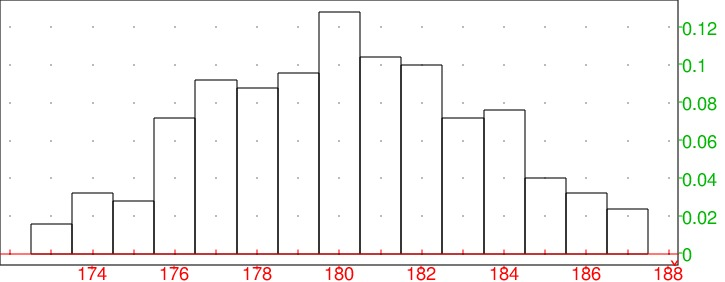
\includegraphics[width=\textwidth]{stathisto}\\
On tape :\\
{\tt diagramme\_batons([[T],[Ef]])}\\
On obtient :\\
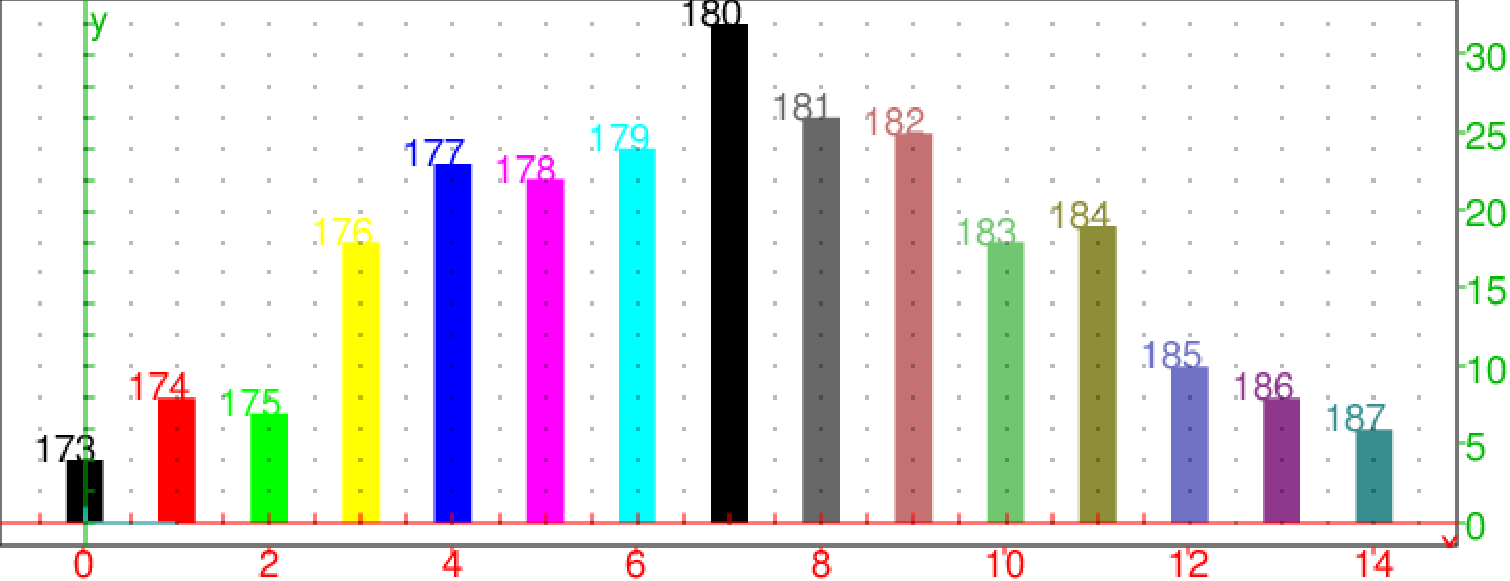
\includegraphics[width=\textwidth]{statdiag}\\
On tape :\\
{\tt moustache([T],[Ef])}\\
On obtient :\\
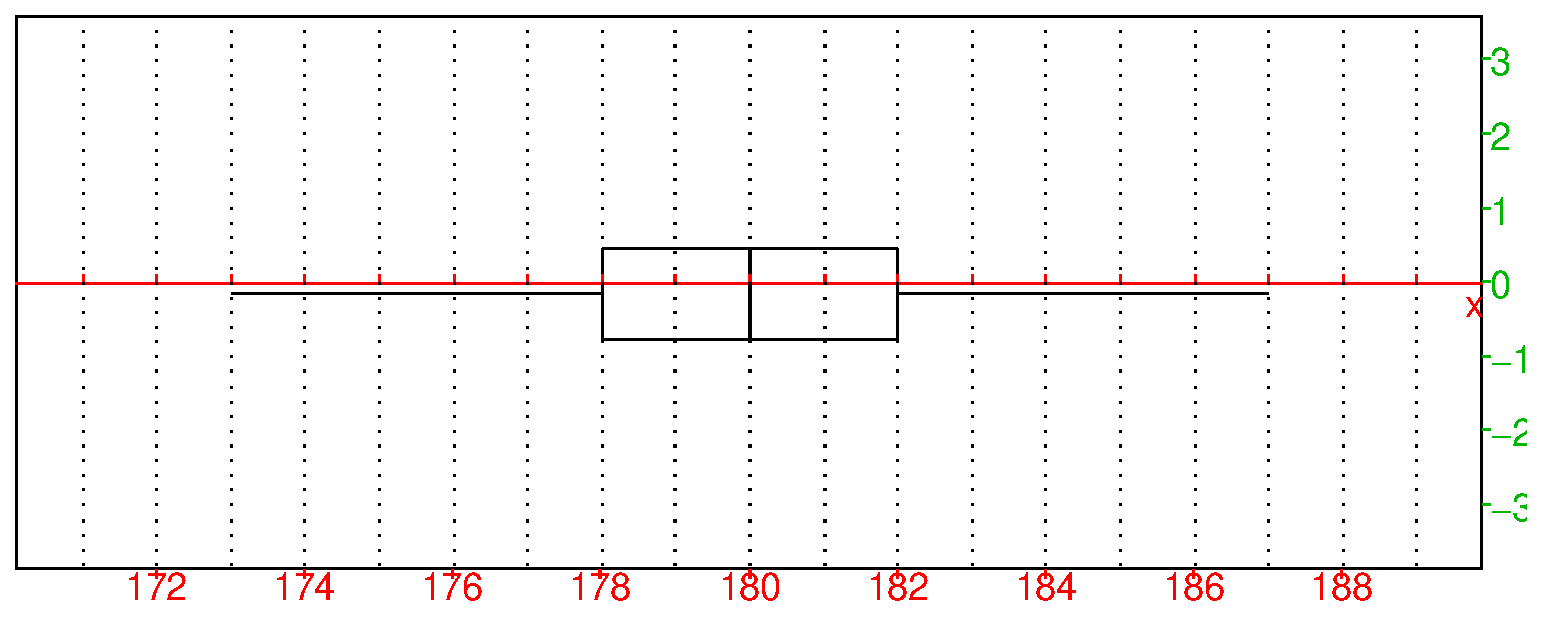
\includegraphics[width=\textwidth]{statmoust}\\
On tape :\\
{\tt Efc:=(sum(Ef[j],j=0..k)/250.)\$(k=0..size(Ef)-1)}\\
On obtient :\\
{\tt 0.016,0.048,0.076,0.148,0.24,0.328,0.424,0.552,0.656,0.756,0.828,0.904,0.944,0.976,1.0}\\
On tape :\\
{\tt affichage(nuage\_points([[T],[Efc]])), point\_point+epaisseur\_point\_2),frequences\_cumulees(tran([[T],[Ef]]))}\\
On obtient :\\
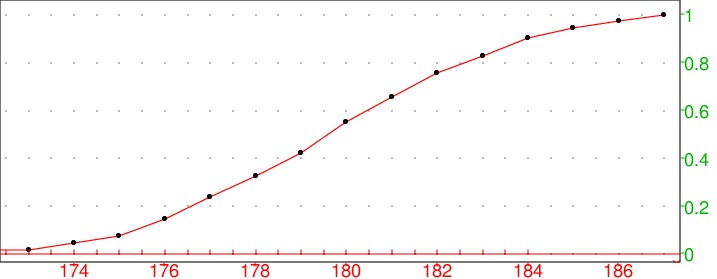
\includegraphics[width=\textwidth]{statfreq}\\
On tape :\\
{\tt approx(mean([T],[Ef]))}\\
On obtient :\\
{\tt 180.104}\\
On tape :\\
{\tt approx(sttdev([T],[Ef]))}\\
On obtient :\\
{\tt 3.27859482096}\\
On tape :\\
{\tt histogramme(tran([[T],[Ef]])),\\
plotfunc(loi\_normale(180.104,3.27859482096,x),x=172..188),\\
nuage\_points(tran([[T],[Ef]/250.]),affichage=1+point\_point+epaisseur\_point\_2)}\\
On obtient :\\
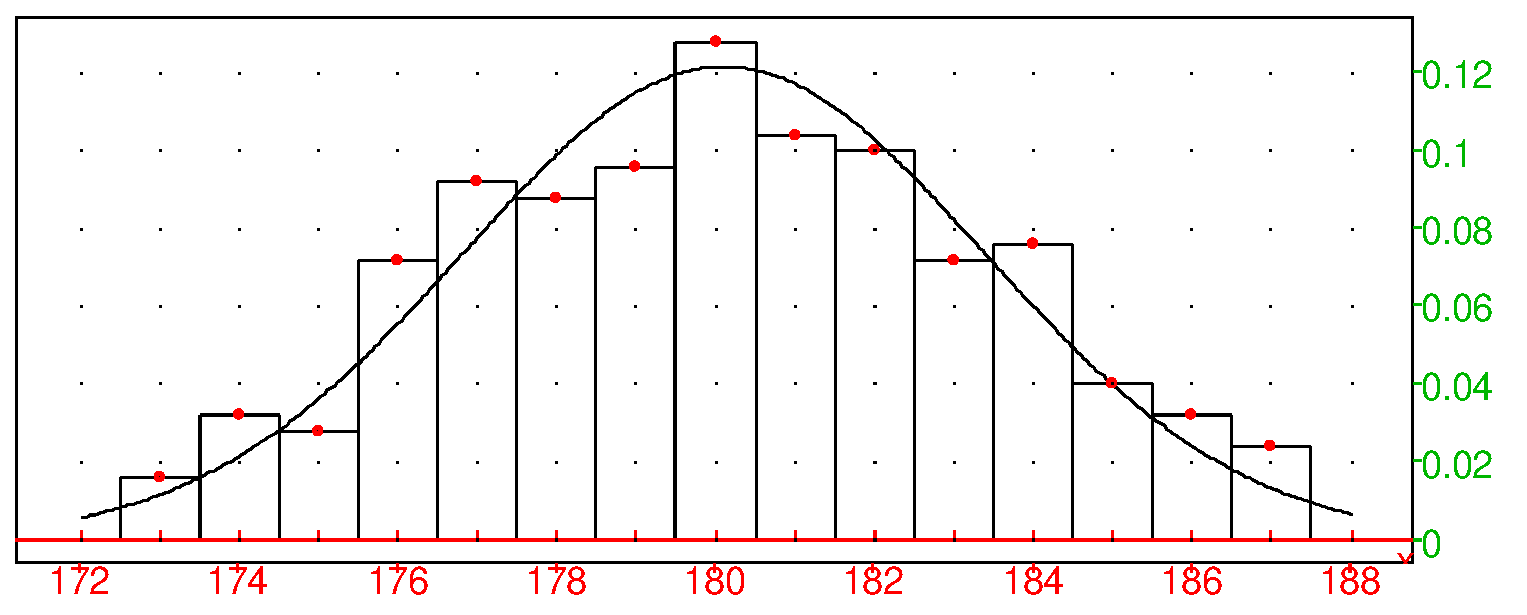
\includegraphics[width=\textwidth]{statnormal}
\subsection{Vocabulaire des s\'eries quantitatives \`a 1 variable}
Soit une s\'erie quantitative \`a 1 variable {\tt L}.\\
La diff\'erence entre la plus grande valeur et la plus petite valeur du 
caract\`ere effectivement obtenue est l'{\bf \'etendue} de la s\'erie {\tt L}.\\
Le nombre de membres de la population \'etudi\'ee est l'{\bf effectif total}.\\
Si le caract\`ere est discret, il est commode d'indiquer pour chaque valeur du 
caract\`ere, le nombre des membres de la population ayant cette valeur : c'est 
l'{\bf effectif de cette valeur}.\\ 
Si le caract\`ere est continu, on partage l'intervalle sur lequel s'\'etendent
ces valeurs en intervalles (en g\'en\'eral \'egaux) que l'on appelle 
{\bf classe}. Le nombre des membres de la population ayant leur valeur dans une
 classe est l'{\bf effectif de cette classe}.\\ 
La valeur moyenne des bornes d'une classe est le {\bf centre} de cette 
classe.\\
L'{\bf effectif cumul\'e} d'une valeur (ou d'une classe) est la somme de
l'effectif de cette valeur (ou de cette classe) et de tous les effectifs des 
valeurs (ou des classes) qui pr\'ec\`edent.\\
 La {\bf fr\'equence} d'une valeur (ou d'une classe) est le rapport de  
l'effectif de cette valeur (ou de cette classe) par l'effectif total.\\
Avec {\tt Xcas} on tape par exemple :\\
{\tt frequences([1,2,1,1,2,1,2,4,3,3])}\\
On obtient ;\\
{\tt [[1,0.4],[2,0.3],[3,0.2],[4,0.1]]}\\
La {\bf fr\'equence cumul\'ee} d'une liste de valeurs (ou d'une classe) est la 
somme de la fr\'equence de cette valeur (ou de cette classe) et de toutes les 
fr\'equences des valeurs (ou des classes) qui la pr\'ec\`edent.\\
Avec {\tt Xcas} on tape par exemple :\\
{\tt frequences\_cumulee([[0.75,30],[1.75,50],[2.75,20]])}\\
ou \\
{\tt frequences\_cumulee([[0.25..1.25,30],[1.25..2.25,50],}\\
{\tt [2.25..3.25,20]])}\\
On obtient le diagramme des fr\'equences cumul\'ees.\\
L'{\bf histogramme} des effectifs (resp fr\'equences) d'un caract\`ere discret 
ou continu est le graphique qui permet de visualiser l'effectif (resp 
fr\'equences) des diff\'erentes valeurs du caract\`ere : on met en abscisse les
diff\'erentes valeurs  du caract\`ere (ou le centre des diff\'erentes classes),
puis on forme des rectangles accol\'es deux \`a deux, ses  rectangles ont deux 
cot\'es parrall\'eles \`a l'axe des ordonn\'ees,
le  cot\'e port\'e par l'axe des abscisses a pour longueur l'amplitude de la 
classe, et l'autre est  tel que l'aire du rectangle est \'egale \`a l'effectif 
(resp fr\'equences) de la valeur consid\'er\'ee.\\  
L'{\bf histogramme des fr\'equences} permet de visualiser les fr\'equences des 
diff\'erentes classes au moyen de la surface de rectangles : chaque rectangle 
correspond \`a une classe et a  pour surface la fr\'equence de cette classe.\\
Avec {\tt Xcas} on tape par exemple :\\
{\tt histogramme([[0.75,30],[1.75,50],[2.75,20]])}\\
ou \\
{\tt histogramme([[0.25..1.25,30],[1.25..2.25,50],}\\
{\tt [2.25..3.25,20]])}\\
On obtient un histogramme des fr\'equences.\\  
La {\bf fonction de r\'epartition des fr\'equences} est \'egale pour chaque 
valeur du caract\`ere \`a la fr\'equence cumul\'ee de cette valeur.\\
Le {\bf mode} est la valeur du caract\`ere dont l'effectif est le plus grand.\\
Le {\bf maximum} est la plus grande valeur du caract\`ere effectivement 
obtenue.\\
Le {\bf minimum} est la plus petite valeur du caract\`ere effectivement 
obtenue.\\
La {\bf m\'ediane}  partage la s\'erie statistique en deux groupes de m\^eme 
effectif. C'est une valeur du caract\`ere \`a partir de laquelle
 l'effectif des valeurs qui lui sont inf\'erieures est superieur ou \`egal \`a 
l'effectif des valeurs qui lui sont sup\'erieures (par exemple
la m\'ediane de [140,145,146,147] est 146 et la m\'ediane de [140,145,146] est 
145). La m\'ediane est donc la valeur du caract\`ere \`a partir de laquelle la 
fr\'equence cumul\'ee atteint ou d\'epasse 0.5.\\
Les {\bf quartiles} sont trois valeurs du caract\`ere qui partage la s\'erie 
statistique en quatre groupes de m\^eme effectif :\\
- le {\bf 1-ier quartile} est la valeur du caract\`ere \`a partir de laquelle 
la fr\'equence cumul\'ee atteint ou d\'epasse 0.25.\\
- le {\bf 2-i\`eme quartile} est confondu avec la m\'ediane.\\ 
- le {\bf 3-i\`eme quartile} est la valeur du caract\`ere \`a partir de 
laquelle la fr\'equence cumul\'ee atteint ou d\'epasse 0.75.\\
On peut d\'efinir les {\bf d\'eciles}. Il y a 9 d\'eciles :\\
le {\bf 1-ier d\'ecile} est la valeur du caract\`ere \`a partir de laquelle la 
fr\'equence cumul\'ee atteint ou d\'epasse 0.1.\\
le {\bf 2-i\`eme d\'ecile} est la valeur du caract\`ere \`a partir de laquelle 
la fr\'equence cumul\'ee atteint ou d\'epasse 0.2.\\
etc...\\
le {\bf 9-i\`eme d\'ecile} est la valeur du caract\`ere \`a partir de laquelle 
la fr\'equence cumul\'ee atteint ou d\'epasse 0.9.\\
On peut aussi d\'efinir le {\bf centile} (il y a 99 centiles) et le 
{\bf  quantile}  d'ordre {\bf p} :\\
le {\bf 1-ier centile} est la valeur du caract\`ere \`a partir de laquelle la 
fr\'equence cumul\'ee atteint ou d\'epasse 0.01.\\
etc...\\
le {\bf 99-i\`eme centile} est la valeur du caract\`ere \`a partir de laquelle 
la fr\'equence cumul\'ee atteint ou d\'epasse 0.99.\\
Le {\bf quantile} d'ordre {\bf p} ({\bf p} un r\'eel de [0,1[), est la valeur 
du caract\`ere \`a partir de laquelle la fr\'equence cumul\'ee atteint ou 
d\'epasse {\bf p}.\\
Le {\bf semi-interquartile}  est \'egal \`a $\frac{1}{2}(Q_3-Q_1)$ o\`u 
$Q_1$ et $Q_3$ d\'esigne le premier et le troisi\`eme quartile. Cet indice 
fournit un renseignement sur l'\'etalement des valeurs de part et d'autre de la
m\'ediane.\\
L'{\bf interquartile}  est \'egal \`a $Q_3-Q_1$ o\`u 
$Q_1$ et $Q_3$ d\'esigne le premier et le troisi\`eme quartile. Cet indice 
fournit un renseignement sur l'\'etalement des valeurs de part et d'autre de la
m\'ediane.\\
L'{\bf interd\'ecile}  est \'egal \`a $D_9-D_1$ o\`u 
$D_1$ et $D_9$ d\'esigne le premier et le neuvi\`eme d\'ecile. Cet indice 
fournit un renseignement sur l'\'etalement des valeurs de part et 
d'autre de la m\'ediane.\\
{\bf Exemples avec {\tt Xcas}}\\
On tape :\\
{\tt L:=[1,2,3,4,5,6,7,8,9,10]}\\
{\tt min(L)} et on obtient {\tt 1 }\\
{\tt  quartile1(L)} et on obtient {\tt 3.0 }\\
{\tt median(L)} et on obtient {\tt 5.0}\\
{\tt  quartile3(L)} et on obtient {\tt 8.0 }\\
{\tt max(L)} et on obtient {\tt 10 }\\
{\tt quartiles(L)} pour avoir le r\'esultat des 5 commandes pr\'ec\'edentes 
 et on obtient {\tt [[1.0],[3.0],[5.0],[8.0],[10.0]]}\\
{\tt quantile(L,0.9)} et on obtient {\tt 9.0}\\
La {\bf boite \`a moustaches} \index{moustache}\index{boxwhisker}
permet de visualiser ces diff\'erentes valeurs :\\
c'est un rectangle dont un cot\'e est un trait allant de $Q_1$ \`a $Q_3$ sur 
lequelle un trait vertical indique la valeur de la m\'ediane et d'o\`u
deux traits horizontaux (les moustaches) d\'ebordent : l'un  va de la valeur 
minimum \`a $Q_1$ et l'autre de $Q_3$ \`a la valeur maximum. 
Sur ces deux moustaches, on trouvent quelquefois deux traits verticaux 
indiquant la valeur du premier et du neuvi\`eme d\'ecile.\\
Avec {\tt Xcas} on tape :\\
{\tt L:=[1,2,3,4,5,6,7,8,9,10]}\\
{\tt moustache(L)}\\
Cela ouvre le graphique et dessine une boite \`a moustaches o\`u on peut 
lire que :\\
Q2=m\'ediane=5, Q1=3, Q3=8, minimum=1, maximum=10.\\

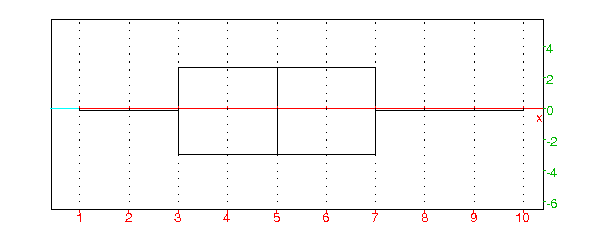
\includegraphics[width=\textwidth]{moustache}

La {\bf moyenne} est le quotient de la somme des valeurs du caract\`ere (pas
toujours distinctes) par l'effectif total.
Si le caract\`ere prend $n$ valeurs distinctes $x_k$ d'effectifs $e_k$ pour
$k=0...(n-1)$ alors l'effectif total vaut $N=\sum_{k=0}^{n-1} e_k$ et 
la moyenne $m$ est :
$\displaystyle m=\frac{1}{N}\sum_{k=0}^{n-1} e_kx_k$.\\
La {\bf variance} est la moyenne des carr\'es des \'ecarts \`a la moyenne des 
valeurs du caract\`ere.
Si le caract\`ere prend $n$ valeurs distinctes $x_k$ d'effectifs $e_k$ 
($k=0...(n-1)$), si la moyenne vaut $m$ et, si l'effectif total vaut $N$ alors
 la variance $v=s^2$ est :
$\displaystyle s^2=\frac{1}{N}\sum_{k=0}^{n-1} e_k(x_k-m)^2=\frac{1}{N}(\sum_{k=0}^{n-1} e_kx_k^2)-m^2$.\\
L'{\bf \'ecart-type} $s$ est la racine carr\'ee de la variance.\\
Soit une s\'erie statistique quantitative d'effectif {\tt N} \`a 1 variable, 
un {\bf \'echantillon d'ordre n} d\'esigne le syst\`eme des $n$ valeurs 
prises par le caract\`ere au cours de $n$ tirages ind\'ependants. Les valeurs 
prises par l'\'echantillon sont donc les valeurs prises par $n$ variables 
al\'eatoires $X_1,...,X_n$ qui suivent la m\^eme loi que la variable 
al\'eatoire $X$ \'egale \`a la valeur du caract\`ere \'etudi\'e.
Par exemple, si dans une ville de {\tt N} habitants, on \'etudie la taille 
(exprim\'ee en centim\`etres) de ses habitants, la taille de 100 personnes 
prises au hasard dans cette ville est un \'echantillon d'ordre 100.
En g\'en\'eral, on ignore la loi de la variable al\'eatoire \'egale \`a la 
taille des habitants de cette ville, et on veut 
d\'egager un certain nombre d'\'el\'ements caract\'eristiques de cette variable
 gr\^ace \`a l'\'echantillon.
%mean    :[6.0] stddev :[3.162] min :[1.0]
%decile1  :[2.0]
%quartile1:[3.0]
%median   :[6.0]
%quartile3:[8.0]
%decile9  :[10.0]
%max      :[10.0]
\section{S\'erie statistique quantitative \`a 2 variables}
\subsection{D\'efinition}
Lorsque pour une population donn\'ee, on \'etudie deux caract\`eres qui sont
exprimables chacun directement par un nombre, 
l'\'enum\'eration des couples de nombres exprimant les valeurs de ces deux 
caract\`eres pour chaque
membre de la population \'etudi\`ee est une 
{\bf s\'erie statistique quantitative \`a 2 variables}.\\
Exemple :\\
Dans une classe de Terminale S, si \`a chaque \'el\`eve on associe son poids 
(en kilogrammes) et sa taille (en centim\`etres), on obtient une 
s\'erie statistique \`a 2 variables. 
\subsection{Vocabulaire des s\'eries quantitatives \`a 2 variables}
Soit une s\'erie statistique quantitative d'effectif {\tt N}, \`a 2 variables, 
un {\bf \'echantillon d'ordre n} d\'esigne le syst\`eme des $n$ couples de 
valeurs prises par ces 2 variables au cours de $n$ tirages ind\'ependants.
Par exemple, si dans une ville de {\tt N} habitants on \'etudie la taille et le
poids de ses habitants, la taille et le poids de 100 personnes prises au hasard
est un \'echantillon de statistique \`a 2 variables d'ordre 100. 
On essaye de d\'eterminer si ces 2 variables sont ind\'ependantes
en calculant par exemple leur coefficient de corr\'elation.
\subsection{Moyennes, variances, covariances d'effectif 1}
Soit une s\'erie statistique \`a deux variables d'ordre $n$ 
pour les caract\`eres $X$ et $Y$ repr\'esent\'ee par les couples $(x_j,\ y_j)$ 
 pour $0 \leq j \leq (n-1)$.\\
Ici les $x_j$ (resp $y_j$) ne sont pas forc\'ement distincts.\\
La moyenne de $X$ est : $\bar x= \frac{1}{n}\sum_{j=0}^{n-1} x_j$.\\
La moyenne de $Y$ est : $\bar y= \frac{1}{n}\sum_{j=0}^{n-1} y_j$.\\
La variance de $X$ est : $\sigma^2(X)= \frac{1}{n}\sum_{j=0}^{n-1} (x_j-\bar x)^2 =\frac{1}{n}\sum_{j=0}^{n-1} x_j^2-\bar x^2$.\\
La variance de $Y$ est : $\sigma^2(Y)= \frac{1}{n}\sum_{j=0}^{n-1} (y_j-\bar y)^2 =\frac{1}{n}\sum_{j=0}^{n-1} y_j^2-\bar y^2$.\\
La covariance de $(X,Y)$ est :\\
 $cov(X,Y)= \frac{1}{n}\sum_{j=0}^{n-1} (x_j-\bar x)(y_j-\bar y) =\frac{1}{n}\sum_{j=0}^{n-1} x_jy_j-\bar x\bar y$.
\subsection{Moyennes, variances, covariances avec effectifs}
Soit une s\'erie statistique \`a deux variables d'ordre $n$ 
pour les caract\`eres $X$ et $Y$ repr\'esent\'ee par les couples $(x_j,\ y_k)$ 
d'effectifs $n_{j,k}$
($0 \leq j \leq (p-1)$ et $0 \leq k \leq (q-1)$).\\
Ici les $x_j$ (resp $y_k$) sont distincts.\\
Soit $n=\sum_{j=0}^{p-1}\sum_{k=0}^{q-1}n_{j,k}$\\
La moyenne de $X$ est : \\
$\bar x= \frac{1}{n}\sum_{j=0}^{p-1} (x_j*\sum_{k=0}^{q-1}n_{j,k})$.\\
La moyenne de $Y$ est : \\
$\bar y= \frac{1}{n}\sum_{k=0}^{q-1} (y_k*\sum_{j=0}^{p-1}n_{j,k})$.\\
La variance de $X$ est : \\
$\sigma^2(X)= \frac{1}{n}\sum_{j=0}^{p-1} ((x_j-\bar x)^2 *(\sum_{k=0}^{q-1}n_{j,k}))=\frac{1}{n}\sum_{j=0}^{p-1} (x_j^2*\sum_{k=0}^{q-1}n_{j,k})-\bar x^2$.\\
La variance de $Y$ est : \\
$\sigma^2(Y)= \frac{1}{n}\sum_{k=0}^{q-1} ((y_k-\bar y)^2*( \sum_{j=0}^{p-1}n_{j,k}))=\frac{1}{n}\sum_{k=0}^{q-1} (y_k^2*\sum_{j=0}^{p-1}n_{j,k})-\bar y^2$.\\
La covariance de $(X,Y)$ est : \\
$cov(X,Y)= \frac{1}{n}\sum_{j=0}^{p-1} \sum_{k=0}^{q-1}(x_j-\bar x)(y_k-\bar y)
n_{j,k} =\frac{1}{n}\sum_{j=0}^{n-1} \sum_{k=0}^{q-1}x_jy_kn_{j,k}-\bar x\bar y$.
\subsection{Corr\'elation statistique}
Rappel : Lorsqu'on a deux variables al\'eatoires $X$ et $Y$, 
de covariance  $cov(X,Y)$  et  d'\'ecart-type respectif  ${\tt\sigma(X)}$
et ${\tt \sigma(Y)}$ on d\'efinit leur coefficient de corr\'elation 
$\rho(X,Y)$ par :
\begin{center}$\displaystyle \rho(X,Y)=\frac{cov(X,Y)}{\sigma(X)\sigma(Y)}$\end{center}
Supposons que l'on a relev\'e des valeurs $(x_j,y_j)$ de {\tt X} et {\tt Y} au
cours de $n$ \'epreuves ind\'ependantes. On d\'efinit, par analogie, un 
coefficient de corr\'elation $r(X,Y)$ de l'\'echantillon par :\\
\begin{center}$\displaystyle r(X,Y)=\frac{cov(X,Y)}{s(X)s(Y)}$\end{center} 
o\`u $s(X)$ (resp $s(Y)$) d\'esigne l'\'ecart-type des valeurs de $X$ 
(resp $Y$) pour l'\'echantillon. On a :\\
\begin{center}$r(X,Y)=\frac{\frac{1}{n}\sum_{j=0}^{n-1} x_jy_j-\frac{1}{n}\sum_{j=0}^{n-1} x_j*\frac{1}{n}\sum_{j=0}^{n-1} y_j}{\sqrt{\frac{1}{n}\sum_{j=0}^{n-1} (x_j-\frac{1}{n}\sum_{k=0}^{n-1} x_k)^2}*\sqrt{\frac{1}{n}\sum_{j=0}^{n-1} (y_j-\frac{1}{n}\sum_{k=0}^{n-1} y_k)^2}}$\end{center}
{\bf Propri\'et\'es }:\\
$-1 \leq \rho \leq +1$\\
si $X$ et $Y$ sont ind\'ependants alors $\rho(X,Y)=0$ mais la 
r\'eciproque est fausse.
\subsection{Les fonctions {\tt covariance} et {\tt correlation} de {\tt Xcas}} 
On se reportera aussi aux sections \ref{sec:cov}, \ref{sec:corr} et 
\ref{sec:corre}.\\
Avec {\tt Xcas} on tape :
\begin{center}{\tt covariance([1,2],[11,13,14],[[3,4,5],[12,1,2]])}\end{center}
On obtient :
\begin{center}{\tt -83/243}\end{center}
Avec {\tt Xcas} on tape :
\begin{center}{\tt correlation([1,2],[11,13,14],[[3,4,5],[12,1,2]])}\end{center}
On obtient :
\begin{center}{\tt -83/160}\end{center}
\subsection{Ajustement lin\'eaire}\index{scatterplot}\index{linear\_regression}
On se reportera aussi aux sections \ref{sec:linreg} et \ref{sec:expreg}.\\
Une s\'erie statistique \`a deux variables d'ordre $n$ fournit un nuage de $n$
 points. Ajuster lin\'eairement cet ensemble de points consiste \`a trouver une
droite qui approche "le mieux possible le nuage de points".
Un ajustement lin\'eaire va permettre de faire des pr\'evisions ou d'estimer 
des valeurs.

 {\bf Premi\`ere droite des moindres carr\'es} est d\'efinie pour que la somme
 des carr\'es des \'ecarts 
en ordonn\'ee entre les mesures et les points de cette droite soit minimale.\\
Soient $A_j$ ($0 \leq j \leq n-1$) les points de coordonn\'ees $(x_j,\ y_j)$ 
formant le nuage de points.
Soit $D$ une droite d'\'equation $y=ax+b$ et soient $B_j$  pour 
$0 \leq j \leq (n-1)$ les points de $D$ de coordonn\'ees $(x_j,\ ax_j+b)$.\\
On cherche $a$ et $b$ pour que :\\
$S=\sum_{j=0}^{n-1}(y_j-ax_j-b)^2$ soit minimum. \\
Pour $a$ fix\'e le minimum de $S$ est atteint lorsque la droite $D$ passe par 
le point moyen $G$ de coordonn\'ees ($\bar x,\ \bar y)$) donc lorsque
$b=b_0=\bar y-a \bar x$.\\
On trouve ensuite que pour $b=b_0$,  $S$ est minimum pour :\\
$\displaystyle a=a_0=\frac{\frac{1}{n}\sum_{j=0}^{n-1}x_j y_j-\bar x\bar y}
{\frac{1}{n}\sum_{j=0}^{n-1}x_j^2-\bar x^2} =\frac{cov(X,Y)}{\sigma^2(X)}$.\\
La premi\`ere droite des moindres carr\'es est la droite d'\'equation 
$y=a_0x+b_0$. Elle a donc pour \'equation 
$\displaystyle y=\bar y+\frac{cov(X,Y)}{\sigma^2(X)}(x-\bar x)$.

{\bf Deuxi\`eme droite des moindres carr\'es} est d\'efinie pour que la somme
 des carr\'es des \'ecarts 
en abscisse entre les mesures et les points de cette droite soit minimale.\\
On change simplement le r\^ole de $X$ et de $Y$.
On trouve la droite $\Delta$ d'\'equation :\\
$\displaystyle x=\bar x+\frac{cov(X,Y)}{\sigma^2(Y)}(y-\bar y)$.

Avec {\tt Xcas} on tape dans une ligne d'entr\'ee de g\'eom\'etrie, pour tracer
le nuage de points :\\
{\tt scatterplot([[1,11],[1,13],[1,14],[2,11],[2,13],}\\
{\tt [2,14]])}.\\
ou on tape : \\
{\tt scatterplot([1,1,1,2,2],[11,13,14,11,13])}\\
Ou dans le tableur, on s\'electionne l'argument et on utilise le menu 
{\tt Statistiques} du tableur puis {\tt 2d} et {\tt Scatterplot}.\\
On tape dans une ligne d'entr\'ee, pour avoir l'\'equation de la droite des 
moindres carr\'es :\\
%{\tt linear\_regression([[1,11],[1,13],[1,14],[2,11],[2,13],}\\
%{\tt [2,14]]) }
%ou on tape : \\
{\tt linear\_regression([1,1,1,2,2],[11,13,14,11,13])}\\
On obtient :\\
{\tt -2/3,40/3}


\section{Les th\'eor\`emes des statistiques inf\'erentielles}
\subsection{Probl\`emes de jugement sur \'echantillon}
%Exploitations des donn\'ees}
L'exploitation des donn\'ees peut prendre plusieurs formes :

a/ L'inf\'erence statistique ou "th\'eorie de l'estimation" : connaissant un 
\'echantillon, on d\'esire \'emettre une estimation sur la population totale.
Dans ce cas, on n'a pas d'id\'ee a priori sur le param\`etre \`a estimer : \\
on construira
{\bf un intervalle de confiance  $I_\alpha$ au seuil $\alpha$}.\\
Cet intervalle $I_\alpha$ d\'epend de l'\'echantillon et contient, en 
g\'en\'eral, la valeur du param\`etre sauf dans $\alpha \%$ des cas c'est \`a
dire, il y a 
seulement $\alpha \%$ des \'echantillons qui ont un $I_\alpha$ qui ne contient
pas le param\`etre (on dit 
qu'on a un risque d'erreur \'egal \`a $\alpha$).

b/ Le test d'hypoth\`eses permet de savoir si il y a accord entre th\'eorie et
 exp\'erience.
Dans ce cas on a une id\'ee a priori sur la valeur que doit avoir le
 param\`etre : on construit le test d'hypoth\`eses (deux hypoth\`eses $H_0$ et 
$H_1$ seront en concurrence), puis on pr\'el\`eve un 
\'echantillon et on regarde si cet \'echantillon v\'erifie le test ce qui 
permet d'accepter ou de refuser l'hypoth\`ese privil\'egi\'ee $H_0$.\\
Par exemple : on veut contr\^oler qu'une fabrication correspond 
bien \`a ce qui a \'et\'e d\'ecid\'e, pour cela on fabrique un test
d'hypoth\`eses, puis on teste l'hypoth\`ese $H_0$ sur un \'echantillon de la 
production.\\
c/ Le test d'homog\'en\'eite permet de comparer une distribution
exp\'erimentale \`a une distribution th\'eorique.\\
{\bf Remarque} :\\
 en a/ et en b/ on a seulement comparer ou estimer des valeurs 
caract\'eristiques comme fr\'equences ou moyennes, en c/ on compare deux 
distributions.

%c/ La th\'eorie de la d\'ecision : cette th\'eorie ne sera pas abord\'ee ici.
%\section{M\'ethode statistique}
\subsection{Th\'eor\`eme de Bienaym\'e-Tchebychef}
{\bf Th\'eor\`eme} La probabilit\'e pour qu'une variable al\'eatoire $X$ 
diff\`ere de sa moyenne (en valeur absolue) d'au moins $k$ fois son \'ecart 
type, est au plus \'egale \`a $1/k^2$, c'est \`a dire si $X$  a comme moyenne
$m=E(X)$ et comme \'ecart type $\sigma$ on a :
$Proba(|X-m| \geq k \sigma)\leq \frac{1}/{k^2}$
{\bf Exemples}
\begin{itemize}
\item On lance 100 fois un d\'e et on consid\`ere comme \'ev\'enement :\\
on obtient 6 ou on n'obtient pas 6.\\
Par l'exp\'erience on a obtenu $n_1$ fois le nombre 6
Trouver  un majorant de  $Proba(|n_1/100-1/6| \geq 1/10)$.

La probabilit\'e d'avoir un 6 est : $p=1/6$ et de ne pas avoir un 6 est 5/6.\\
Si $Y$ est la variable al\'eatoire \'egale \`a la fr\'equence de 
l'\'ev\'enement favorable on a $E(Y)=p=1/6 \simeq 0.166666666667$ et 
$\sigma(Y)=sqrt(1/6*5/6/100)=sqrt(5)/60 \simeq 0.037267799625$
Th\'eor\`eme de Bienaym\'e-Tchebychef nous dit que :\\
$Proba(|n_1/100-1/6| \geq k \sigma(Y))\leq \frac{1}/{k^2}$\\
On cherche $k$ pour avoir $k \sigma(Y)= k sqrt(5)/60\leq 1/10$\\
on prend $k=2.6832815732$ car $k\leq 6/sqrt(5)\simeq 2.683281573$\\
donc $Proba(|n_1/100-1/6| \geq 1/10)<1/2.68^2\simeq 0.139$\\
Cela veut dire que : $n_1/100$ se trouve dans l'intervalle \\
$1/6-1/10\simeq 0.0666666666667;1/6+1/10 \simeq 0.266666666667$ avec la 
probabilit\'e $1-0.139=0.861$ ou encore que $n_1$ se trouve dans l'intervalle
$6; 26$ avec la probabilit\'e 0.861.

\item m\^eme exercice mais cette fois on lance le d\'e 6000 fois.\\
Par l'exp\'erience on a obtenu $n_1$ fois le nombre 6
Trouver  un majorant de  $Proba(|n_1/6000-1/6| \geq 1/100)$.

Si $Y$ est la variable al\'eatoire \'egale \`a la fr\'equence de 
l'\'ev\'enement favorable on a $E(Y)=p=1/6 \simeq 0.166666666667$ et 
$\sigma(Y)=sqrt(1/6*5/6/6000)=sqrt(5/60)/60 \simeq 0.00481125224325$
On cherche $k$ pour avoir $k \sigma(Y)= k sqrt(5/60)/60\leq 1/100$\\
on prend $k=2.07846096908$ car $k\leq 6/sqrt(50/6)\simeq 2.07846096908$\\
donc $Proba(|n_1/6000-1/6| \geq 1/100)<1/2.07846096908^2\simeq 0.231481481482$\\
Cela veut dire que : $n_1/6000$ se trouve dans l'intervalle \\
$1/6-1/100\simeq 0.16566666666667;1/6+1/10 \simeq 0.176666666667$ avec la 
probabilit\'e $1-0.231481481482=0.768518518518$ ou encore que $n_1$ se 
trouve dans l'intervalle $940; 1060$ avec la probabilit\'e de 0.768518518518.
{\bf Remarque} En approchant la loi binomiale par la loi normale de moyenne
$n*p=6000*1/6=1000$ et d'\'ecart type 
$\sigma=sqrt(np(1-p)=sqrt(6000*1/6*5/6)\simeq 28.8675134595$
On a $60/28.8675134595=2.07846096908$
On cherche dans une table $\psi(t)=Prob(0<T<t)=\psi(2.07846096908)$ et on 
trouve 0.481. Donc $Prob(-t<T<t)=2*0.481=0.962$
ou dans une table $\Pi(t)=Prob(-\infty<T<t)=\Pi(2.07846096908)$ et on 
trouve 0.981. Donc $Prob(-t<T<t)=2*0.981-1=0.962$
donc  $n_1$ se trouve dans l'intervalle
$940; 1060$ avec la probabilit\'e de 0.481*2=0.962.

\item On extrait 1000 fois avec remise une carte d'un jeu de 32 cartes
et on consid\`ere comme \'ev\'enement :\\
on obtient un as ou on n'obtient pas un as.\\
Par l'exp\'erience on a obtenu $n_1$ fois un as
Trouver  un minorant de  $Proba(105<n_1<145)$.

La probabilit\'e d'avoir un as est : p=1/8 et de ne pas avoir un as est 7/8.
Si $Y$ est la variable al\'eatoire \'egale \`a la fr\'equence de 
l'\'ev\'enement favorable on a $E(Y)=p=1/8=0.125$ et 
$\sigma(Y)=sqrt(1/8*7/8/1000)=sqrt(7/10)/80\simeq 0.0104582503317$.
On a $Proba(105<n_1<145)=Proba(|n_1-125|<20)=Proba(|n_1/1000-0.125|<1/50)$
Le th\'eor\`eme de Bienaym\'e-Tchebychef nous dit que :\\
$Proba(|n_1/1000-1/8| \geq k \sigma(Y))\leq \frac{1}/{k^2}$\\
On choisit $k \sigma(Y)=1/50$ c'est \`a dire 
$k=1/50/0.0104582503317=1.91236577493$ donc $1/k^2=0.273437500001$
Cela veut dire que 
$Proba(|n_1/1000-0.125|<1/50) \geq 0.273437500001$ donc\\
$Proba(105<n_1<145) \leq 1-0.273437500001=0.7265625$
{\bf Remarque} 
$Proba(|n_1/1000-0.125|>1/100) \geq 1/0.956182887465^2=1.09375000001$
ce qui ne nous apporte rien!
\end{itemize}
\subsection{Loi des grands nombres}
{\bf Notation} \\
On note ici $\displaystyle \bar X_n=\frac{X_1+X_2+..+X_n}{n}$
pour bien faire ressortir que $\bar X_n$ d\'epend de $n$,
mais quelquefois dans la suite on \'ecrira simplement :
$\displaystyle \bar X=\frac{X_1+X_2+..+X_n}{n}$ pour ne pas alourdir les 
notations.

{\bf Loi faible des grands nombres} :\\
Soient $X_1$, $X_2$,.., $X_n$ des variables al\'eatoires ind\'ependantes de 
moyenne $\mu_1$, $\mu_2$,.., $\mu_n$ et d'\'ecart-type $\sigma_1$, 
$\sigma_2$,.., $\sigma_n$.\\
Si quand $n$ tend vers l'infini 
$\frac{1}{n} \sum _{j=1}^n \mu_j $ tend vers $\mu$ et,\\
 si quand $n$ tend vers 
l'infini  $\frac{1}{n^2} \sum _{j=1}^n \sigma_j^2$ tend vers $0$,\\
 alors  
$\displaystyle \bar X_n=\frac{X_1+X_2+..+X_n}{n}$ converge en probabilit\'e 
vers $\mu$ quand $n$ tend vers l'infini (i.e. pour tout $\epsilon$ et pour tout
$\eta$ il existe $n_0$ tel que pour tout $n>n_0$ on
a $Proba(|\bar X_n-\mu|>\epsilon)<\eta$).\\
Cas des \'echantillons :\\
Si $X_1$,$X_2$,..,$X_n$ sont un \'echantillon de $X$ de moyenne $\mu$ et 
d\'ecart-type $\sigma$, on a  $\mu_1=\mu_2=..=\mu_n=\mu$ et 
$\sigma_1= \sigma_2=..=\sigma_n=\sigma$. 
Donc $\frac{1}{n} \sum _{j=1}^n \mu_j =\mu$ et quand $n$ tend vers l'infini 
$\frac{1}{n^2} \sum _{j=1}^n \sigma_j^2 =\frac{\sigma^2}{n}$ tend vers $0$ 
ce qui montre que la variable al\'eatoire \\
$\displaystyle \bar X_n=\frac{X_1+X_2+..+X_n}{n}$ converge en probabilit\'e 
vers $\mu$ quand $n$ tend vers l'infini.\\

{\bf Loi forte des grands nombres} :\\
Soient $X_1$, $X_2$,.., $X_n$ des variables al\'eatoires ind\'ependantes de 
moyenne $\mu_1$, $\mu_2$,.., $\mu_n$ et d'\'ecart-type $\sigma_1$, $\sigma_2$
,.., $\sigma_n$.\\
 Si quand $n$ tend vers l'infini $\frac{1}{n} \sum _{j=1}^n \mu_j $ tend vers 
$\mu$ et,\\
si $\sum _{j=1}^\infty \frac{\sigma_j^2}{j^2}$ est convergente,\\
alors  $\displaystyle  \bar X_n=\frac{X_1+X_2+..+X_n}{n}$ converge presque 
s\^urement vers $\mu$ quand $n$ tend vers l'infini (i.e. dire que $Y_n$ 
converge  presque s\^urement vers $U$ c'est dire que l'ensemble des points de 
divergene est de probabilit\'e nulle i.e.\\
 $Proba(\omega, \lim_{n \rightarrow +\infty}(Y_n(\omega) \neq U(\omega))=0$).\\
Cas des \'echantillons :\\
Si $X_1$,$X_2$,..,$X_n$ sont un \'echantillon de $X$ de moyenne $\mu$ et 
d\'ecart-type $\sigma$, on a $\mu_1=\mu_2=..=\mu_n=\mu$ et $\sigma_1= \sigma_2=..=\sigma_n=\sigma$.\\ 
Donc  $\frac{1}{n} \sum _{j=1}^n \mu_j =\mu$ et 
$\displaystyle\sum _{j=1}^\infty \frac{\sigma^2}{j^2} =\sigma^2\sum _{j=1}^\infty\frac{1}{j^2}$ est convergente ce qui montre que :\\
$\displaystyle \bar X_n=\frac{X_1+X_2+..+X_n}{n}$ converge presque s\^urement
 vers $\mu$ quand $n$ tend vers l'infini.\\
 
{\bf Le th\'eor\`eme central-limite} :\\
Quand $n$ tend vers l'infini, alors\\
$\displaystyle \bar Y_n=\sqrt n \frac{(\bar X_n-\mu)}{\sigma}$ converge en 
loi vers $U$ variable al\'eatoire qui suit la loi normale centr\'ee r\'eduite 
(dire que $Y_n$ converge en loi vers $U \in \mathcal N(0,1)$ veut dire que si 
$F$ est la fonction 
de r\'epartition de la loi normale centr\'ee r\'eduite et si $F_n$ est la 
fonction de r\'epartition de $Y_n$ alors pour tout $x\in \mathbb{R}$, $F_n(x)$
tend vers $F(x)$ quand $n$ tend vers l'infini).
\subsection{Moyenne et variance empirique}
Soit un  \'echantillon d'effectif $n$ et $(x_1,x_2,...,x_n)$ les $n$ valeurs
 observ\'ees. \\
La moyenne empirique est :\\
$\displaystyle m=\frac{x_1+x_2+...+x_n}{n}$\\
La variance empirique est :\\
$\displaystyle s^2=\frac{(x_1-m)^2+...+(x_n-m)^2}{n}$\\

Soit un  \'echantillon de taille $n$.\\
 Les $n$ valeurs observ\'ees 
$(x_1,x_2,...,x_n)$ du 
caract\`ere sont consid\'er\'ees comme \'etant les valeurs de $n$ 
variables al\'eatoires ind\'ependantes $X_1,X_2,..,X_n$ suivant la  
m\^eme loi $F$ d'esp\'erance 
${\tt \mu}$ et d'\'ecart-type ${\tt \sigma}$.

L'ensemble des moyennes d'\'echantillons de taille $n$ est la variable 
al\'eatoire $\displaystyle \bar X=\frac{X_1+X_2+..+X_n}{n}$.\\
Si le r\'esultat observ\'e est $x_1,x_2..x_n$, alors la valeur observ\'ee
 de $\bar X$ est la moyenne empirique $m$ :\\
$ \displaystyle m=\frac{x_1+x_2+..+x_n}{n}$.

L'ensemble des variances d'\'echantillons de taille $n$ est la variable 
al\'eatoire $\displaystyle S^2=\frac{(X_1-\bar X)^2+(X_2-\bar X)^2+..+(X_n-\bar X)^2}{n}$.\\
Si le r\'esultat observ\'e est $ x_1,x_2..x_n$, alors  la 
valeur observ\'ee de $S^2$ est la variance 
empirique $s^2$ :\\
$\displaystyle s^2=\frac{(x_1-m)^2+(x_2-m)^2+..+(x_n-m)^2}{n}$.
\subsection{\'Etude de ${\tt \bar X}$}
{\bf Th\'eor\`emes}\\
La variable al\'eatoire $\displaystyle  \bar X=\frac{X_1+X_2+..+X_n}{n}$
converge en probabilit\'e vers $\mu$.\\
De plus $ \bar X$ a pour  moyenne ${\tt \mu}$ et pour variance $\displaystyle \frac{\sigma^2}{n}$.\\
Quand $n$ tend vers l'infini, $\displaystyle \sqrt n \frac{(\bar X-\mu)}{\sigma}$ converge en 
loi vers $U$ variable al\'eatoire qui suit la loi normale centr\'ee r\'eduite.
\subsection{Estimateur de $\mu$}\label{sec:estimu}
On appelle estimateur de $\mu$, une variable al\'eatoire $U_n$ fonction d'un 
\'echantillon $X_1$,$X_2$,..,$X_n$ qui v\'erifie :\\
$\lim_{n->\infty} E(U_n)=\mu$ et $\lim_{n->\infty}\sigma^2(U_n)=0$\\
On dit que $U_n$ est un  estimateur {\bf sans biais} de $\mu$ si c'est un  
estimateur de $\mu$ qui v\'erifie $E(U_n)=\mu$.\\ 
{\bf Th\'eor\`eme}\\
$\displaystyle  \bar X=\frac{(X_1+X_2+..+X_n)}{n}$
 est un  estimateur sans biais de $\mu$.
\subsection{\'Etude de ${\tt S^2}$}
{\bf Th\'eor\`eme}\\
La variable  $\displaystyle S^2=\frac{(X_1-\bar X)^2+(X_2-\bar X)^2+..+(X_n-\bar X)^2}{n}$
 converge presque s\^urement vers $\sigma^2$ quand $n$ tend vers l'infini.\\
De plus $  S^2$ a pour  moyenne :\\
  $\displaystyle  E(S^2)=\frac{n-1}{n}\sigma^2$ \\
et pour variance :\\
$\displaystyle  \sigma^2(S^2)= V(S^2)=\frac{n-1}{n^3}((n-1)\mu_4-(n-3)\sigma^4)$ o\`u
$\mu_4=E((X-\mu)^4)$.\\

{\bf Th\'eor\`eme limite pour $S^2$} :\\\
Quand $n$ tend vers l'infini, $\displaystyle \sqrt n \frac{(S^2-\frac{n-1}{n}\sigma^2)}{\sqrt{\mu_4-\sigma^4}}$ converge en 
loi vers $U$ variable al\'eatoire qui suit la loi normale centr\'ee r\'eduite 
(dire que $Y_n$ converge en loi vers $U \in \mathcal N(0,1)$ veut dire que si 
$F$ est la fonction de r\'epartition de la loi normale centr\'ee r\'eduite et 
si $F_n$ est la fonction de r\'epartition de $Y_n$ alors pour tout $x\in \mathbb{R}$, $F_n(x)$ tend vers $F(x)$ quand $n$ tend vers l'infini).
\subsection{Estimateur de $\sigma^2$}\label{sec:estims}
On appelle estimateur de $\sigma^2$, une variable al\'eatoire $V_n$ fonction 
d'un \'echantillon $X_1$,$X_2$,..,$X_n$ qui v\'erifie :\\
$\lim_{n->\infty} E(V_n)=\sigma^2$ et $\lim_{n->\infty}\sigma^2(V_n)=0$\\
On dit que $V_n$ est un  estimateur {\bf sans biais} de $\sigma^2$ si c'est un
estimateur de $\sigma^2$ qui v\'erifie $E(V_n)=\sigma^2$.\\ 
{\bf Th\'eor\`eme}\\
$\displaystyle Z^2=\frac{(X_1-\mu)^2+..+(X_n-\mu)^2}{n}$
 est un  estimateur sans biais de $\sigma^2$.\\
 $\displaystyle S^2=\frac{(X_1-\bar X)^2+..+(X_n-\bar X)^2}{n}$ est un  
estimateur de $\sigma^2$.\\ 
 $\displaystyle \frac{n}{n-1}S^2=\frac{(X_1-\bar X)^2+..+(X_n-\bar X)^2}{n-1}$ 
est un  estimateur sans biais 
de $\sigma^2$.\\
En effet :\\
Pour $S^2$ cela d\'ecoule des th\'eor\`emes pr\'ec\'edents.\\
 Pour $Z^2$ on a :\\
$E(Z^2)=\frac{1}{n}\sum_{j=1}^n E((X_j-\mu)^2)=\frac{1}{n}n\sigma^2=\sigma^2$\\
et puisque $\sigma^2(X-\mu)^2=E((X-\mu)^4)-(\sigma^2)^2=\mu_4-(\sigma^2)^2$ 
on a :\\
$\sigma^2(Z^2)=\frac{1}{n}(\mu_4-(\sigma^2)^2)$ (o\`u $\mu_4=E((X-\mu)^4)$ est 
le moment centr\'e d'ordre 4).\\
{\bf Remarque} :\\
\`A partir des valeurs $x_1,x_2,..,x_n$ de l'\'echantillon, on utilisera 
lorsqu'on connait $\mu$,  $\displaystyle \frac{(x_1-\mu)^2+(x_2-\mu)^2+..+(x_n-\mu)^2}{n}$ 
comme estimateur de $\sigma^2$ et si $\mu$ est inconnu on utilisera comme 
estimateur de $\sigma^2$
$\displaystyle \frac{(x_1-m)^2+(x_2-m)^2+..+(x_n-m)^2}{n-1}$ avec
$\displaystyle m=\frac{x_1+x_2+..+x_n}{n}$. 
\subsection{En r\'esum\'e}
Le probl\`eme est d'obtenir, au vu de l'\'echantillon empirique, des 
renseignements sur la population dont l'\'echantillon  est issu (c'est \`a dire
sur la population parente de moyenne $\mu$ et d'\'ecart-type $\sigma$), en 
particulier sur la valeur de sa moyenne ${\tt \mu}$.\\
En g\'en\'eral $\sigma$ n'est pas connu, on prend faute de mieux, quand $n$ est
grand :\\ 
$\sigma=s \sqrt {\frac{n}{n-1}}$ o\`u $ s^2$ est la valeur 
observ\'ee de :\\
$\displaystyle S^2=\frac{(X_1-Y)^2+(X_2-Y)^2+..+(X_n-Y)^2}{n}$ qui a pour  
moyenne  $\displaystyle \frac{n-1}{n}\sigma^2$.\\
Gr\^ace au th\'eor\`eme central-limite, la variable $\displaystyle \bar X=\frac{X_1+..+X_n}{n}$  va nous servir \`a trouver une valeur de $\mu$ car :\\
$\bar X$ a pour  moyenne $\mu$ et  pour variance 
$\displaystyle \frac{\sigma^2}{n} \simeq \frac{s^2}{n-1}$ donc la 
variable al\'eatoire :\\  
$\displaystyle \sqrt n \frac{(\bar X-\mu)}{\sigma}\simeq \sqrt {n-1} \frac{(\bar X-\mu)}{s}$ converge en 
loi vers $ U \in \mathcal N(0,1)$.\\
\section{Les tests d'hypoth\`eses}
Concernant une variable al\'eatoire $X$, on souhaite comparer la valeur
 effective d'un param\`etre $p$ \`a une valeur attendue $p_0$. Il s'agit de 
savoir si la valeur observ\'ee sur un \'echantillon est vraisemblable avec 
$p=p_0$.\\ 
{\bf Test statistique} : proc\'edure conduisant au vu de l'\'echantillon \`a 
rejeter, avec un certain risque d'erreur $\alpha$ une hypoth\`ese que l'on 
cherche \`a tester appel\'ee $H_0$. La proc\'edure de test est fond\'ee sur 
une opposition d'hypoth\`eses et on note $H_1$ l'hypoth\`ese alternative : 
cela veut dire que l'on risque de rejeter \`a tort l'hypoth\`ese $H_0$ avec
 une probabilit\'e \'egale \`a $\alpha$.\\
{\bf Test bilat\'eral} : test pour lequel l'hypoth\`ese $H_0$ est rejet\'ee,
si la statistique utilis\'ee prend une valeur en dehors d'un intervalle.\\
{\bf Test unilat\'eral \`a droite} : test pour lequel l'hypoth\`ese $H_0$ est 
rejet\'ee, si la statistique utilis\'ee prend une valeur sup\'erieure \`a une 
valeur.\\ 
{\bf Test unilat\'eral \`a gauche} : test pour lequel l'hypoth\`ese $H_0$ est 
rejet\'ee, si la statistique utilis\'ee prend une valeur inf\'erieure \`a une 
valeur.\\
{\bf Construction d'un test} :\\
- choix du seuil de risque  $\alpha$,\\ 
- choix des hypoth\`eses $H_0$ et $H_1$,\\
par exemple on choisira un test unilat\'eral \`a droite si on sait \`a priori 
que $p \leq p_0$. On aura alors $H_0$ : $p=p_0$ et  $H_1$ : $p > p_0$,\\
- choix d'une variable statistique $S$ servant de variable de d\'ecision,\\
- d\'etermination de la r\'egion critique au seuil $\alpha$,\\
- \'enonc\'e de la r\`egle de d\'ecision.\\
{\bf Utilisation du test} :\\
- pr\'el\`evement d'un \'echantillon,\\
- au vu de la valeur observ\'ee $s$ de $S$, rejeter ou accepter $H_0$.

{\bf Remarques}\\
Le seuil de risque  $\alpha$ est toujours petit ($\alpha<0.1$) : si on 
demande  un test \`a 95\% cela veut dire que le seuil de 
risque est $\alpha=0.05$.\\
N'oubliez pas que lorsque l'on rejette l'hypoth\`ese  $H_0$ cela veut dire que 
l'hypoth\`ese  $H_0$ risque d'\^etre vraie dans moins de $100*\alpha$ cas pour
100 cas et
 que lorsque l'on accepte l'hypoth\`ese  $H_0$ cela veut dire que 
l'hypoth\`ese  $H_0$ risque d'\^etre vraie dans plus de $100*\alpha$ cas pour
100  cas.
\subsection{\'Etude de la fr\'equence  $p$ d'un caract\`ere $X$}
Soit une variable al\'eatoire $X$ qui suit une loi de Bernouilli de 
param\`etre $p$ (on \'etudie un caract\`ere, si ce caract\`ere est observ\'e 
alors $X=1$ et sinon $X=0$ et on a $Proba(X=1)=p$). Soit $\bar X$ la moyenne 
des \'echantillons de taille $n$ : ici, $\bar X$ est \'egal pour chaque 
\'echantillon de taille $n$ \`a la fr\'equence observ\'ee $F$ du caract\`ere.\\
Si $n$ est grand ($n \geq 30$), $\bar X$ suit approximativement la 
loi normale $\mathcal N(p,\sqrt{\frac{p(1-p)}{n}})$.\\
 Si $n$ est petit, on a  $(n*\bar X)$ suit la loi binomiale 
$\mathcal B(n,p)$.\\
On choisit le seuil $\alpha$ et selon les cas :\\
Test d'hypoth\`eses bilat\'eral : $H_0 : p =p_0$ et  $H_1 : p \neq p_0$\\
Test d'hypoth\`eses unilat\'eral \`a droite (\`a gauche) : $H_0 :p =p_0$ et 
 $H_1:p > p_0$ (resp $H_0 : p =p_0$ et  $H_1:p< p_0$)\\
On calcule, sous l'hypoth\`ese $H_0$, soit au moyen des tables de la loi 
normale (pour $n$ grand, $np(1-p)>7$), soit au moyen des tables de la loi 
binomiale (pour $n$ petit), soit avec {\tt Xcas}, les bornes de l'intervalle 
d'acceptation au seuil $\alpha$, de l'hypoth\`ese $H_0$. 
\begin{itemize}
\item dans le cas bilat\'eral, on cherche les r\'eels 
$a_1$ et $a_2$ v\'erifiant :\\
$Proba(a_1<F=\bar X<a_2)=1-\alpha$\\
- pour $n$ grand, on cherche dans une table de loi centr\'ee r\'eduite $h$ tel 
que $Proba(Y<h)=1-\alpha/2$, on pose \\
$F=(Y-p_0)/\sqrt{\frac{p_0(1-p_0)}{n}}$ 
et on obtient :\\
$Proba(F<p_0+h*\sqrt{\frac{p_0(1-p_0)}{n}})=1-\alpha/2$, donc \\
$a_1=p_0-h*\sqrt{\frac{p_0(1-p_0)}{n}}$ et
$a_2=p_0+h*\sqrt{\frac{p_0(1-p_0)}{n}}$\\
On peut aussi taper dans {\tt Xcas} si $\alpha=0.05$ :\\
{\tt a1:=normal\_icdf(p0,sqrt((p0*(1-p0)/n),0.025)}\\
{\tt a2:=normal\_icdf(p0,sqrt(p0*(1-p0)/n),0.975)}\\
- pour $n$ petit, $n*F$ suit la loi binomiale $\mathcal B(n,p_0)$,
 on cherche dans une table de 
loi binomiale $\mathcal B(n,p_0)$ les valeurs $n*p_1$ et $n*p_2$ tels que :\\
$Proba( n*p_1<n*F<n*p_2)=1-\alpha$\\
et donc :\\
$Proba(p_1<F<p_2)==1-\alpha$\\
On peut aussi taper dans {\tt Xcas} si $\alpha=0.05$ :\\
{\tt p1:=1/n*binomial\_icdf(n,p0,0.025)}\\
{\tt p2:=1/n*binomial\_icdf(n,p0,0.975)}\\

\item  dans le cas unilat\'eral \`a droite, on cherche le r\'eel 
$a$ v\'erifiant :\\
$Proba(F<a)=1-\alpha$ :\\
- pour $n$ grand, on cherche dans une table de loi centr\'ee r\'eduite $h$ tel 
que $Proba(Y<h)=1-\alpha$, on a alors $Proba( F<p_0+h\sqrt{\frac{p_0(1-p_0)}{n}})=1-\alpha$ donc $a=p_0+h\sqrt{\frac{p_0(1-p_0)}{n}}$ \\
On peut aussi taper dans {\tt Xcas}  si $\alpha=0.05$ :\\
{\tt a:=normal\_icdf(p0,sqrt(p0*(1-p0)/n),0.975)}\\
- pour $n$ petit, on cherche $n*p_2$ tel que :\\
$Proba(n*F<n*p_2)=1-\alpha$\\
on a donc $Proba(F<p_2=1-\alpha$\\
On peut aussi taper dans {\tt Xcas}  si $\alpha=0.05$ :\\
{\tt p2:=1/n*binomial\_icdf(n,p0,0.975)}\\

\item  dans le cas unilat\'eral \`a gauche, on cherche le r\'eel 
$b$ v\'erifiant :\\
$Proba(F<b)=\alpha$ :\\
- pour $n$ grand, on cherche dans une table de loi centr\'ee r\'eduite $h$ tel 
que $Proba(Y<h)=\alpha$, on a alors $Proba( F<p_0+h\sqrt{\frac{p_0(1-p_0)}{n}})=\alpha$ donc\\
 $b=p_0+h\sqrt{\frac{p_0(1-p_0)}{n}}$ \\ 
On peut aussi taper dans {\tt Xcas}  si $\alpha=0.05$ :\\
{\tt b:=normal\_icdf(p0,sqrt(p0*(1-p0)/n),0.05)}\\
- pour $n$ petit, on cherche $n*p_1$ tel que :\\
$Proba(n*F< n*p_1)=\alpha$\\
on a donc :\\
$Proba(F<p_1)=\alpha$\\
On peut aussi taper dans {\tt Xcas}  si $\alpha=0.05$ :\\
{\tt p1:=1/n*binomial\_icdf(n,p0,0.05)}
\end{itemize}
{\bf R\`egle de d\'ecision} :\\
Soit la fr\'equence $f$ d'un \'echantillon de taille $n$.\\
On rejette l'hypoth\`ese $H_0$ au seuil $\alpha$ :
\begin{itemize}
\item dans le cas bilat\'eral\\ 
si $f\not\in [a_1;a_2]$, (ou si $f\not\in [p_1;p_2]$) 
\item dans le cas unilat\'eral \`a droite\\
si $f>a$, (ou si $f>p_2$)
\item dans le cas unilat\'eral \`a gauche\\
si $f<b$, (ou si $f<p_1$)
\end{itemize}
sinon on accepte l'hypoth\`ese $H_0$ au seuil $\alpha$.\\
{\bf Exemple}\\
On choisit $n=30$, $p_0=0.3$ et $\alpha=0.05$ et on compare les r\'esultats de 
la loi normale et de la loi binomiale.\\
\begin{itemize}
\item dans le cas bilat\'eral \\
Pour  $n=30$ et  $H_0\  : \ p=0.3$ $H1\  :\  p \neq 0.3$ et $\alpha=0.05$\\
on a $p_0*(1-p_0)=0.3*0.7=0.21$ et on tape :\\
{\tt normal\_icdf(0.3,sqrt(0.21/30),0.975)=0.463982351931}\\
{\tt normal\_icdf(0.3,sqrt(0.21/30),0.025)=0.136017648069}\\
on pose $I=[0.1360;0.464]$\\
ou on tape :\\
{\tt 1/30*binomial\_icdf(30,0.3,0.025)=2/15}\\
{\tt 1/30*binomial\_icdf(30,0.3,0.975)=7/15}\\
on pose $I=[0.1333;0.46666]$\\
On rejette $H_0$ au seuil de 5\%, si la fr\'equence $f$ obtenue \`a partir 
d'un \'echantillon de taille $n=30$ est en dehors de l'intervalle $I$.
\item  dans le cas unilat\'eral \`a droite\\
Pour  n=30 $H_0 :p=0.3$ $H1 : p \geq 0.3$ et $\alpha=0.05$\\
on a $p_0*(1-p_0)=0.3*0.7=0.21$ et on tape :\\
{\tt normal\_icdf(0.3,sqrt(0.21/30),0.95)=0.437618327917}\\
on pose $I=]-\infty;0.464]$\\
ou on tape :\\
{\tt 1/30*binomial\_icdf(30,0.3,0.95)=13/30}\\
on pose  $I=]-\infty;0.43334]$\\
On rejette $H_0$ au seuil de 5\%, si la fr\'equence $f$ obtenue \`a partir 
d'un \'echantillon de taille $n=30$ est en dehors de l'intervalle $I$.
\item  dans le cas unilat\'eral \`a gauche\\
Pour  n=30 $H_0 :p=0.3$ $H1 : p \leq 0.3$ et $\alpha=0.05$\\
on a $p_0*(1-p_0)=0.3*0.7=0.21$ et on tape :\\
{\tt normal\_icdf(0.3,sqrt(0.21/30),0.05)=0.162381672083}\\
on pose $I=[0.16238;+\infty[$\\
ou on tape :\\
{\tt 1/30*binomial\_icdf(30,0.3,0.05)=1/6}\\
on pose $I=[0.166667;+\infty[$\\
On rejette $H_0$ au seuil de 5\%, si la fr\'equence $f$ obtenue \`a partir 
d'un \'echantillon de taille $n=30$ est en dehors de l'intervalle $I$.
\end{itemize}
\subsection{\'Etude de la valeur moyenne $\mu$ d'un caract\`ere $X$}
On va faire des tests d'hypoth\`eses sur $\mu$ c'est \`a dire que dans ce qui 
suit, on suppose que $\mu=\mu_0$, ie que l'on connait $\mu$. 
\subsubsection{$n$ est grand ($n > 30$)}
{\bf Th\'eor\`emes} :\\
Si $X \in \mathcal N(\mu,\sigma)$ alors 
$\bar X\in \mathcal N(\mu,\sigma/\sqrt n)$. \\
Si $X$ suit une loi quelconque et si l'\'echantillon est de grande taille 
($n>30$), $\bar X$ suit approximativement une loi $\mathcal N(\mu,\sigma/\sqrt n)$.\\  
- si l'\'ecart-type $\sigma$ est connu, on connait la loi suivie par $\bar X$,\\
- si l'\'ecart-type $\sigma$ n'est pas connu, puisque $n$ est grand on va 
pouvoir estimer $\sigma$ par $s\sqrt{n/(n-1)}$ o\`u $s$ 
est l'\'ecart-type  d'un \'echantillon de taille $n$ et on se ram\'ene 
au cas pr\'ecedent ($\sigma$ connu) en prenant $\sigma=s\sqrt{n/(n-1)}$.
Ainsi on connait la loi suivie par $\bar X$ : $\bar X$ suit approximativement 
une loi $N(\mu,s/\sqrt {n-1})$.\\ 
{\bf Recette quand on connait la loi $\mathcal N(\mu,\sigma/\sqrt n)$ 
suivie par $\bar X$} ($\sigma$ connu)\\ 
On choisit le seuil $\alpha$ et selon les cas :\\
Test d'hypoth\`eses bilat\'eral : $H_0 :\mu =\mu_0$  et  $H_1:\mu\neq \mu_0$\\
Test d'hypoth\`eses unilat\'eral \`a droite : $H_0 :\mu =\mu_0$ et  $H_1:\mu> \mu_0$ (resp \`a gauche : $H_0 :\mu =\mu_0$ et  $H_1:\mu< \mu_0$)\\
On calcule,  au moyen des tables de loi normale ($n$ grand, $n>30$) les bornes 
de l'intervalle d'acceptation au seuil $\alpha$, 
de l'hypoth\`ese $H_0$.
\begin{itemize} 
\item  dans le cas bilat\'eral, on cherche les r\'eels 
$a_1$ et $a_2$ v\'erifiant :\\
$Proba(a_1<\bar X<a_2)=1-\alpha$ :\\
on cherche dans une table de loi centr\'ee r\'eduite $h$ tel que :\\
$Proba(Y<h)=1-\alpha/2$, on a $Proba(\bar X<\mu_0+h*\sigma/\sqrt n)=1-\alpha/2$, donc \\
$a_1=\mu_0-h*\sigma/\sqrt n$ et
$a_2=\mu_0+h*\sigma/\sqrt n$\\
Avec {\tt Xcas}, on tape :\\
{\tt a1:=normal\_icdf($\mu_0,\frac{\sigma}{\sqrt n},\alpha/2$)}\\
{\tt a2:=normal\_icdf($\mu_0,\frac{\sigma}{\sqrt n},1-\alpha/2$)}
\item  dans le cas unilat\'eral \`a droite, on cherche le r\'eel 
$a$ v\'erifiant :\\
$Proba(\bar X<a)=1-\alpha$ :\\
on cherche dans une table de loi centr\'ee r\'eduite $h$ tel que :\\
$Proba(Y<h)=1-\alpha$, on a $Proba(\bar X<\mu_0+h*\sigma/\sqrt n)=1-\alpha$,
 donc \\
$a=\mu_0+h*\sigma/\sqrt n$.\\ 
Avec {\tt Xcas}, on tape :\\
{\tt a:=normal\_icdf($\mu_0,\frac{\sigma}{\sqrt n},1-\alpha$)}
\item dans le cas unilat\'eral \`a gauche, on cherche le r\'eel 
$b$ v\'erifiant :\\
$Proba(\bar X<b)=\alpha$ :\\
on cherche dans une table de loi centr\'ee r\'eduite $h$ tel que :\\
$Proba(Y<h)=\alpha$, on a alors $Proba(\bar X<\mu_0+h*\sigma/\sqrt n)=\alpha$, 
donc \\
$b=\mu_0+h*\sigma/\sqrt n$.\\ 
Avec {\tt Xcas}, on tape :\\
{\tt b:=normal\_icdf($\mu_0,\frac{\sigma}{\sqrt n },\alpha$)}
\end{itemize}
{\bf R\`egle de d\'ecision} :\\
Soit $m$ la moyenne d'un \'echantillon de taille $n$.\\
On rejette l'hypoth\`ese $H_0$ au seuil $\alpha$ :
\begin{itemize}
\item dans le cas bilat\'eral\\ 
si $m \not\in [a_1;a_2]$,
\item dans le cas unilat\'eral \`a droite\\
si $m>a$,
\item dans le cas unilat\'eral \`a gauche\\
si $m<b$, 
\end{itemize}
sinon on accepte l'hypoth\`ese $H_0$ au seuil $\alpha$.

\subsubsection{$X \in \mathcal N(\mu,\sigma)$ et $n$ est petit,  ($n\leq30$)}
On a deux cas selon que l'\'ecart-type $\sigma$ est connu ou pas : \\
- si l'\'ecart-type $\sigma$ est connu\\
On sait que si $X \in \mathcal N(\mu,\sigma)$ alors 
$\bar X\in \mathcal N(\mu,\sigma/\sqrt n)$  on se reportera \`a la "Recette 
quand on connait la loi $\mathcal N(\mu,\sigma/\sqrt n)$ suivie par $\bar X$"
 \'ecrite ci-dessus.\\
- si l'\'ecart-type $\sigma$ est inconnu\\
Lorsque $n$ est petit, on ne peut plus approcher $\sigma$ par $s\sqrt{n/(n-1)}$
 o\`u $s$ est l'\'ecart-type  d'un \'echantillon de taille $n$.\\ 
C'est pourquoi, lorsque $n$ est petit et que $X \in \mathcal N(\mu,\sigma)$, on
utilise la statistique :
$T=\sqrt{n-1}(\frac{\bar X-\mu_0}{S})$ o\`u 
$S^2=1/n \sum_{j=1}^n(X_j-\bar X)^2$.\\
$T$ suit une loi de Student \`a $n-1$ degr\'es de libert\'e et $T$ ne d\'epend 
pas de $\sigma$. \\
{\bf Recette quand on ne connait pas la loi suivie par $\bar X$}\\ 
On est dans le cas o\`u 
$\sigma $ est inconnu, $X \in \mathcal N(\mu,\sigma)$ et $n$ est petit.\\
On choisit le seuil $\alpha$ et selon les cas :\\
Test d'hypoth\`eses bilat\'eral : $H_0 :\mu =\mu_0$ et  $H_1 : \mu\neq \mu_0$\\
Test d'hypoth\`eses unilat\'eral \`a droite : $H_0 :\mu =\mu_0$ et  
$H_1:\mu> \mu_0$ (resp \`a gauche : $H_0 :\mu =\mu_0$ et  $H_1:\mu< \mu_0$).\\
Au moyen des tables de la loi de
Student ($n$ petit, $n \leq 30$)  
\begin{itemize}
\item dans le cas bilat\'eral, on cherche le nombre r\'eel $h$ v\'erifiant : \\
$Proba(-h<T_{n-1}<+h)=1-\alpha$\\
Avec {\tt Xcas}, on tape  si $\alpha=0.05$ :\\
{\tt h:=student\_icdf(n-1,0.975)}
\item dans le cas unilat\'eral \`a droite, on cherche le nombre r\'eel $h_1$ 
v\'erifiant :\\
$Proba( T_{n-1}<h_1)=1-\alpha$\\
Avec {\tt Xcas}, on tape  si $\alpha=0.05$ :\\
{\tt h1:=student\_icdf(n-1,0.95)}
\item dans le cas unilat\'eral \`a gauche, on cherche le nombre r\'eel $h_2$ 
v\'erifiant :\\
$Proba(T_{n-1}<h_2)=\alpha$\\
Avec {\tt Xcas}, on tape  si $\alpha=0.05$ :\\
{\tt h2:=student\_icdf(n-1,0.05)}
\end{itemize}
{\bf R\`egle de d\'ecision} :\\
Soit  $t$  la valeur prise par $T$ par un \'echantillon de taille $n$ :
$\displaystyle t=\sqrt{n-1}(\frac{m-\mu_0}{s})$ o\`u $m$ est la moyenne de 
l'\'echantillon et $s$ son \'ecart-type.\\
On rejette l'hypoth\`ese $H_0$ au seuil $\alpha$ :
\begin{itemize}
\item dans le cas bilat\'eral\\ 
si $t\not\in [-h;+h]$, 
\item dans le cas unilat\'eral \`a droite\\
si $t>h_1$,
\item dans le cas unilat\'eral \`a gauche\\
si $t<h_2$, 
\end{itemize}
sinon on accepte l'hypoth\`ese $H_0$ au seuil $\alpha$.

\subsubsection{$X$ ne suit pas une loi normale  et  $n$ est  petit}
On ne sait pas faire...

\subsection{\'Etude de l'\'ecart-type $\sigma$ de $X\in \mathcal N(\mu,\sigma)$}
On sait que si $X$ suit une loi normale $\mathcal N(\mu,\sigma)$, les
 statistiques :\\
$\displaystyle Z^2=\frac{1}{n}\sum_{j=1}^n (X_j-\mu)^2$ et \\
$\displaystyle S^2=\frac{1}{n}\sum_{j=1}^n (X_j-\bar X)^2$ \\
sont des estimateurs de $\sigma$, de plus $Z^2$ et  $\frac{n}{n-1}S^2$ sont 
des estimateurs sans biais de $\sigma$ (cf \ref{sec:estims}), car on a 
$E(Z^2)=E(\frac{n}{n-1}S^2)=\sigma$  et $S^2$ ne d\'epend 
pas de $\mu$.\\
On sait  que :\\
la statistique $\displaystyle \frac{nZ^2}{\sigma^2}$ suit 
une loi du $\chi^2$ \`a $n$ degr\'es de libert\'e et que \\
la statistique 
$\displaystyle \frac{nS^2}{\sigma^2}$ suit une loi du $\chi^2$ \`a $(n-1)$ 
degr\'es de libert\'e.\\  
Lorsque $\mu$ est connue, on utilisera la statistique 
$\displaystyle \frac{nZ^2}{\sigma^2}$  comme variable de d\'ecision, et
 si $\mu$ n'est pas connue, on utilisera la statistique 
$\displaystyle \frac{nS^2}{\sigma^2}$ comme variable de d\'ecision.\\
{\bf Recette quand $X$ suit une loi normale $\mathcal N(\mu,\sigma)$}\\ 
On choisit le seuil $\alpha$ et selon les cas :\\
Test d'hypoth\`eses bilat\'eral : $H_0 :\sigma =\sigma_0$ et  $H_1:\sigma \neq \sigma_0$,\\
Test d'hypoth\`eses unilat\'eral \`a droite : $H_0 :\sigma =\sigma_0$ et  $H_1:\sigma > \sigma_0$ (resp  \`a gauche : $H_0 :\sigma =\sigma_0$ et  
$H_1:\sigma < \sigma_0$).\\ 
On calcule au moyen des tables de $\chi^2(n)$
 les nombres r\'eels $h_1$ et $h_2$ v\'erifiant :
\begin{itemize} 
\item dans le cas  bilat\'eral\\
- si la valeur moyenne $\mu$ est connue\\
$Proba(\chi^2_n<h_1)=1-\alpha/2$\\
$Proba(\chi^2_n<h_2)=\alpha/2$\\
Avec {\tt Xcas}, on tape  si $\alpha=0.05$ :\\
{\tt h1:=chisquare\_icdf(n,0.975)}\\
{\tt h2:=chisquare\_icdf(n,0.025)}\\
- si la valeur moyenne $\mu$  n'est pas connue\\
$Proba(\chi^2_{n-1}<h_1)=1-\alpha/2$\\
$Proba(\chi^2_{n-1}<h_2)=\alpha/2$\\
Avec {\tt Xcas}, on tape  si $\alpha=0.05$:\\
{\tt h1:=chisquare\_icdf(n-1,0.975)}\\
{\tt h2:=chisquare\_icdf(n-1,0.025)}\\
\item dans le cas  unilat\'eral \`a droite\\ 
- si la valeur moyenne $\mu$ est connue\\
$Proba(\chi^2_n<h_1)=1-\alpha$\\
Avec {\tt Xcas}, on tape  si $\alpha=0.05$ :\\
{\tt h1:=chisquare\_icdf(n,0.95)}\\
- si la valeur moyenne $\mu$ n'est pas connue\\
$Proba(\chi^2_{n-1}<h_1)=1-\alpha$\\
Avec {\tt Xcas}, on tape :\\
{\tt h1:=chisquare\_icdf(n-1,0.95)}\\
\item dans le cas  unilat\'eral \`a gauche\\
- si la valeur moyenne $\mu$ est connue\\
$Proba(\chi^2_n<h_2)=\alpha$\\
Avec {\tt Xcas}, on tape  si $\alpha=0.05$ :\\
{\tt h2:=chisquare\_icdf(n,0.05)}\\
- si la valeur moyenne $\mu$ n'est pas connue\\
$Proba(\chi^2_{n-1}<h_2)=\alpha$\\
Avec {\tt Xcas}, on tape  si $\alpha=0.05$ :\\
{\tt h2:=chisquare\_icdf(n-1,0.05)}
\end{itemize}
{\bf R\`egle de d\'ecision} :\\
Soit  $u$  la valeur prise par $\displaystyle \frac{nZ^2}{\sigma^2}$ (ou par 
$\displaystyle \frac{nS^2}{\sigma^2}$ si $\mu$ n'est pas connue) pour un 
\'echantillon de taille $n$ :\\
- si $\mu$ est connue, on calcule $\displaystyle u=\frac{\sum_{j=0}^n(x_j-\mu)^2}{\sigma_0^2}$ o\`u les $x_j$ sont les valeurs de l'\'echantillon 
(car selon $H_0 :\sigma =\sigma_0$).\\
- si $\mu$ n'est pas connue, on calcule 
$\displaystyle u=\frac{n*s^2}{\sigma_0^2}$ o\`u  $s$ est l'\'ecart-type de 
l'\'echantillon (car selon $H_0 :\sigma =\sigma_0$).\\
On rejette l'hypoth\`ese $H_0 :\sigma =\sigma_0$ au seuil $\alpha$ :
\begin{itemize}
\item dans le cas bilat\'eral\\ 
si $u\not\in [h_2;h_1]$, 
\item dans le cas unilat\'eral \`a droite\\
si $u>h_1$,
\item dans le cas unilat\'eral \`a gauche\\
si $u<h_2$, 
\end{itemize}
sinon on accepte l'hypoth\`ese $H_0$ au seuil $\alpha$.
\section{Intervalle de confiance}
L'estimation a pour but, \`a partir d'\'echantillons, de donner des valeurs 
num\'eriques aux param\`etres de la population dont ces \'echantillons sont 
issus.\\ 
Il peut s'agir d'estimation ponctuelle ou d'estimation par intervalle.\\
Un intervalle de confiance $I_\alpha$ au seuil $\alpha$, pour le param\`etre 
$p_0$, est un intervalle qui contient $p_0$ avec une confiance  
de $1-\alpha$,  cela veut dire que pour un grand nombre $n$ d'\'echantillons 
environ $n*\alpha$ des $I_\alpha$ ne contiennent pas $p_0$ (en effet les 
intervalles de confiance $I_\alpha$ d\'ependent de l'\'echantillon)
{\tt Remarques}
Le seuil de risque  $\alpha$ est toujours petit ($\alpha<0.1$) : si on vous 
demande un  intervalle de confiance \`a 95\% cela veut dire 
que le seuil de risque est $\alpha=0.05$.\\
N'oubliez pas que l'estimation d'une valeur par un intervalle de confiance
 comporte un risque, celui de situer la valeur dans un intervalle o\`u elle ne 
se trouve pas !!!! (c'est $\alpha$ qui determine le risque d'erreur)\\
Plus on demande un risque faible et plus l'intervalle de confiance est grand.
\subsection{Valeur de la fr\'equence  $p$ d'un caract\`ere $X$}
\subsubsection{Estimation ponctuelle}
Lorsque la taille $n$ de l'\'echantillon est grande, on prend comme estimation 
ponctuelle de $p$ la fr\'equence $f$ observ\'ee sur l'\'echantillon.\\
{\bf Remarque}\\
Cela ne donne aucune information sur la qualit\'e de l'estimation. 
\subsubsection{Estimation par un intervalle}
{\bf Cas des \'echantillons de taille $n>30$}\\
Soit $X$ une variable al\'eatoire de Bernouilli de param\`etre $p$ ($X$ vaut 0 
ou 1 et $Proba(X=1)=p$).\\
Soit $\bar X$ la variable al\'eatoire \'egale \`a la moyenne des valeurs prises
par $X$ pour des \'echantillons de taille $n$. 
On a $\bar X=F$ est \'egal \`a la fr\'equence du nombre d'apparitions de la 
valeur 1 pour chaque \'echantillon de taille $n$, .\\
On sait que $n*F$ suit une loi binomiale $\mathcal B(n,p)$, cette loi est
 proche de la loi normale \\
 $\mathcal N(np,\sqrt{np(1-p)})$ car $n$ est grand ($n>30$).\\
On peut donc consid\'erer que $F$ suit approximativement la loi 
$\mathcal N(p,\sqrt{\frac{p(1-p)}{n}})$.\\
{\bf Recette}\\
- On choisit $\alpha$ (par exemple $\alpha=0.05$),\\
- On cherche \`a l'aide d'une table de loi normale centr\'ee r\'eduite,
$h$ v\'erifiant :\\
$Proba(Y<h)=1-\alpha/2$ pour $Y\in \mathcal N(0,1)$.\\
On a donc en posant $Y=\frac{F-p}{\sqrt{\frac{p(1-p)}{n}}}$ :\\
$Proba(p-h \sqrt{\frac{p(1-p)}{n}}<F<p+h \sqrt{\frac{p(1-p)}{n}} )=1-\alpha$\\
- On calcule la valeur $f$ de $F$ pour l'\'echantillon\\
On a donc $n(f-p)^2<h^2p(1-p)$ c'est \`a dire 
$(h^2+n)p^2-p(h^2+2nf)+nf^2<0$ donc $p$ se trouve \`a l'int\'erieur des 
racines de l'\'equation du second degr\'e :\\
$(h^2+n)x^2-x(h^2+2nf)+nf^2=0$ que 
l'on peut r\'esoudre (calcul du discriminant $\Delta=h^4+(-(4*h^2))*n*f^2+4*h^2*n*f$ etc...)\\
 mais il est plus simple de dire, que l'on peut estimer l'\'ecart-type de
 $n*F$. On a $\sigma(n*F)=\sqrt{np(1-p)}$ que l'on peut estimer par
 $\sqrt{nf(1-f)}\sqrt{\frac{n}{n-1}}$. \\
Donc l'\'ecart-type de $\bar X=F$, 
$\sigma(F)=\sigma(\bar X)=\sqrt{\frac{p(1-p)}{n}}$ peut \^etre estim\'e par \\
$\frac{1}{n}\sqrt{nf(1-f)}\sqrt{\frac{n}{n-1}} =\sqrt{\frac{f(1-f)}{n-1}}$,
donc on a :\\
$Proba(p-h\sqrt{\frac{f(1-f)}{n-1}}\leq f\leq p+h\sqrt{\frac{f(1-f)}{n-1}} )=1-\alpha$\\
ou encore \\
$Proba(f-h\sqrt{\frac{f(1-f)}{n-1}}\leq p\leq f+h\sqrt{\frac{f(1-f)}{n-1}} )=1-\alpha$\\
Si $a_1=f-h\sqrt{\frac{f(1-f)}{n-1}}$ et $a_2=f+h\sqrt{\frac{f(1-f)}{n-1}}$
on a $a_1 \leq p \leq a_2$\\
Avec {\tt Xcas}, on tape  si $\alpha=0.05$ :\\
{\tt a1:=normal\_icdf(f,sqrt(f*(1-f)/(n-1),0.025)}\\
{\tt a2:=normal\_icdf(f,sqrt(f*(1-f)/)n-1,0.975)}\\
{\bf R\'esultat}
$I_{\alpha}=[a_1\ ;\ a_2]$ est un intervalle de confiance de $p$ au seuil 
$\alpha$.\\ 
{\bf Cas des \'echantillons de taille $n\leq 30$}\\
Soit $X$ une variable al\'eatoire de Bernouilli de param\`etre $p$ ($X$ vaut 0 
ou 1 et $Proba(X=1)=p$).\\
Soit la variable al\'eatoire $F=\bar X$.\\
On sait que $nF$ suit une loi binomiale $\mathcal B(n,p)$. 
On utilisera donc une table de la loi binomiale.\\ 
{\bf Recette}\\
- On choisit $\alpha$ (par exemple $\alpha=0.05$)\\
- On calcule la valeur $f$ de $F$ pour l'\'echantillon\\
- On approche $p$ par $f$, ainsi $n*F=n*\bar X\in \mathcal B(n,f)$, on cherche 
$n*p_1$ et $n*p_2$ \`a l'aide d'une table de loi binomiale pour avoir :\\
$Proba(n*F<n*p_1)=1-\alpha/2$ et $Proba(n*F<n*p_2)=\alpha/2$\\
Avec {\tt Xcas}, on tape  si $\alpha=0.05$ :\\
{\tt p1:=1/n*binomial\_icdf(,n,f,0.025)}\\
{\tt p2:=1/n*binomial\_icdf(n,f,0.975)}\\
On a donc :\\
$Proba(p_2<f<p_1)=1-\alpha$.\\
{\bf R\'esultat}\\
$I_{\alpha}=[p_2\ ;\ p_1]$ est un intervalle de confiance de $p$ au seuil 
$\alpha$.
\subsection{Valeur moyenne $\mu$ d'un caract\`ere $X$}
\subsubsection{Estimation ponctuelle}
Lorsque la taille $n$ de l'\'echantillon est grande, on prend comme estimation 
ponctuelle de $\mu$ la  moyenne $m$ observ\'ee sur l'\'echantillon.\\
{\bf Remarque}\\
Cela ne donne aucune information sur la qualit\'e de l'estimation. 
\subsubsection{Estimation par un intervalle}
{\bf Cas des \'echantillons de taille $n>30$}\\
Si $n$ est grand ($n>30$), on connait la loi suivie par $\bar X$ : $\bar X$ 
suit approximativement une loi $\mathcal N(\mu,\sigma/\sqrt{n})$ (ou si 
$\sigma$ n'est pas connu $\bar X$ suit approximativement une loi 
$\mathcal N(\mu,s/\sqrt {n-1})$).\\
{\bf Recette lorsque la loi $\mathcal N(\mu,\sigma/\sqrt{n})$ suivie par
$\bar X$ est connue}\\
- On choisit $\alpha$ (par exemple $\alpha=0.05$).\\
- On calcule la valeur $m$ de $\bar X$ pour l'\'echantillon (ie sa moyenne) et 
si $\sigma$ n'est pas connu, l'\'ecart-type $s$ de l'\'echantillon. \\
- On cherche $h$, dans une table de loi normale centr\'ee r\'eduite,
 pour avoir :\\
$Proba(Y<h)=1-\alpha/2$ pour $Y\in \mathcal N(0,1)$ on a alors :\\
$Proba(\mu-h*\sigma/\sqrt{n}<m<\mu+h*\sigma/\sqrt{n})=1-\alpha$ \\
on a donc :\\
$Proba(m-h*\sigma/\sqrt{n}<\mu<m+h*\sigma/\sqrt{n})=1-\alpha$\\
ou si $\sigma$ n'est pas connu :\\
$Proba(\mu-h*s/\sqrt{n-1}<\bar X<\mu+h*s/\sqrt{n-1})=1-\alpha$\\
on a donc $Proba(m-h*s/\sqrt{n-1}<\mu<m+h*\sigma/\sqrt{n-1})=1-\alpha$.\\
Si $\sigma$ est connu on pose :\\
$a_1=m-h*\sigma/\sqrt{n}$ et $a_2=m+h*\sigma/\sqrt{n}$\\
ou si $\sigma$ n'est pas connu  on pose :\\
$a_1=m-h*s/\sqrt{n-1}$ et $a_2=m+h*s/\sqrt{n-1}$\\
on a $a_1 \leq \mu \leq a_2$\\
Avec {\tt Xcas}, si $\sigma$ est connu, on tape si $\alpha=0.05$ :\\
{\tt a1:=normal\_icdf(m,$\sigma$/sqrt(n),0.025)}\\
{\tt a2:=normal\_icdf(m,$\sigma$/sqrt(n),0.975)}\\
ou si $\sigma$ n'est pas connu, on tape si $\alpha=0.05$ :\\
{\tt a1:=normal\_icdf(m,s/sqrt(n-1),0.025)}\\
{\tt a2:=normal\_icdf(m,s/sqrt(n-1),0.975)}\\
{\bf R\'esultat}\\
$I_{\alpha}=[a_1\ ;\ a_2]$ est un intervalle de confiance de $\mu$ au seuil
 $\alpha$.\\

{\bf Cas des petits \'echantillons issus d'une loi normale}\\
Si $\sigma$ est connu, la loi $\mathcal N(\mu,\sigma/\sqrt{n})$ suivie par 
$\bar X$ est connue et on se reportera donc \`a la recette du paragraphe 
pr\'ec\'edent.\\
Si $\sigma$ n'est pas connu, on note 
$S^2=\frac{1}{n}\sum_{j=1}^n(X_j-\bar X)^2$ alors\\
 $T=(\frac{\bar X-\mu}{S})\sqrt{n-1}$ suit une loi de Student \`a $(n-1)$ degr\'es de libert\'e.\\
 {\bf Recette lorsque $n$ est petit et $X \in \mathcal N(\mu,\sigma)$}\\
- On choisit $\alpha$ (par exemple $\alpha=0.05$).\\
- On calcule la valeur $m$ de $\bar X$ pour l'\'echantillon ($m$ est la moyenne
de l'\'echantillon) et l'\'ecart-type $s$ de l'\'echantillon ($s^2$ est la 
valeur de $S^2$ pour l'\'echantillon). \\
- On cherche $h$, dans une table de Student pour $(n-1)$ degr\'es de libert\'e,
 pour avoir :\\
$Proba(-h<T_{n-1}<h)=Proba(-h<(\frac{\bar X-\mu}{S})\sqrt{n-1}<h)=1-\alpha$ \\
Avec {\tt Xcas}, on tape   si $\alpha=0.05$ :\\
{\tt h:=student\_icdf(n-1,0.975)}\\
puisque $m$ est la valeur de $\bar X$ et $s$ la valeur de $S$ pour 
l'\'echantillon on a :\\ 
$Proba(m-hs/\sqrt{n-1}<\mu<m+hs/\sqrt{n-1})=1-\alpha$.\\
{\bf R\'esultat}\\
$I_{\alpha}=[m-hs/\sqrt{n-1};m+hs/\sqrt{n-1}]$ est un intervalle de confiance 
de $\mu$ au seuil $\alpha$.\\
{\bf Exemple}\\
Pour obtenir un intervalle de confiance de $\mu$ au risque $\alpha=0.05$ et 
$ n-1=4$ on tape :\\
{\tt h:=student\_icdf(4,1-0.05/2)}\\
on obtient :\\
{\tt h=2.7764451052$\simeq$ 2.776} donc :\\
$  m-hs/\sqrt4<\mu< m+hs/\sqrt 4$.\\
On prend un \'echantillon d'effectif $n=5$ ($4=n-1$), pour lequel on trouve :\\
$ m=0.484342422505 $ et 
$s=0.112665383246$\\
On tape :\\
{\tt m:=0.484342422505}\\
{\tt s:=0.112665383246}\\
{\tt  m+h*s/sqrt(4)}\\
On obtient :\\
{\tt 0.64072197445}\\
On tape :\\
{\tt  m-hs/sqrt(4)}\\
{\tt 0.32796287056}.\\
donc un intervalle de confiance de $\mu$ au risque $0.05$ est :\\
$[0.32796287056; 0.64072197445]$
\subsection{Valeur de l'\'ecart-type  $\sigma$ de $X\in \mathcal N(\mu,\sigma)$}
\subsubsection{Estimation ponctuelle}
Lorsque la taille $n$ de l'\'echantillon est grande, on prend comme
estimation ponctuelle de $\sigma$, $s\sqrt{\frac{n}{n-1}}$, o\`u
$s$ est l'\'ecart-type de l'\'echantillon.\\
{\ bf Remarque}\\
Cela ne donne aucune information sur la qualit\'e de l'estimation. 
\subsubsection{Estimation par un intervalle}
{\bf Cas o\`u $\mu$ est connue}\\
On pose $Z^2=\frac{1}{n}\sum_{j=1}^n(X_j-\mu)^2$.
Alors $\displaystyle n\frac{Z^2}{\sigma^2}$ suit une loi du $\chi^2$ \`a $n$ 
degr\'es de libert\'e.\\
{\bf Recette lorsque $\mu$ est connue et $X \in \mathcal N(\mu,\sigma)$}\\
- On choisit $\alpha$ (par exemple $\alpha=0.05$).\\
- On calcule la valeur $z^2=\frac{1}{n}\sum_{j=1}^n(x_j-\mu)^2$ de $Z^2$ pour 
les valeurs $x_j$ de l'\'echantillon.\\ 
- On cherche $t_1$ et $t_2$, dans une table du $\chi^2$ pour $n$ degr\'es de 
libert\'e, pour avoir :\\
$Proba(\chi_n^2<t_1)=Proba(n\frac{Z^2}{\sigma^2}<t_1)=1-\alpha/2$ et\\
$Proba(\chi_n^2<t_2)=Proba(n\frac{Z^2}{\sigma^2}<t_2)=\alpha/2$ \\
Avec {\tt Xcas}, on tape si $\alpha=0.05$ :\\
{\tt t1=chisquare\_icdf(n,0.975)}\\
{\tt t2=chisquare\_icdf(n,0.025)}\\
on a donc 
$Proba(t_2<\frac{nZ^2}{\sigma^2}<t_1)=1-\alpha$.\\
et puisque $z^2$ est la valeur de $Z^2$ pour l'\'echantillon on a:\\ 
$Proba(nz^2/t_1<\sigma^2<nz^2/t_2)=1-\alpha$.\\
{\bf R\'esultat}\\
$I_{\alpha}=[\sqrt{nz^2/t_1}\ ;\ \sqrt{nz^2/t_2}]$ est un intervalle de 
confiance de $\sigma$ au seuil
 $\alpha$.\\

{\bf Cas o\`u $\mu$ n'est pas connue}\\
On pose $S^2=\frac{1}{n}\sum_{j=1}^n(X_j-\bar X)^2$.\\
Alors, $\displaystyle n\frac{S^2}{\sigma^2}$ suit une loi du $\chi^2$ \`a $n-1$ degr\'es de libert\'e.\\
{\bf Recette si $\mu$ n'est pas connue et $X \in \mathcal N(\mu,\sigma)$}\\
- On choisit $\alpha$ (par exemple $\alpha=0.05$).\\
- On calcule la valeur $m$ de $\bar X$ pour l'\'echantillon ($m$ est la 
moyenne de l'\'echantillon) et 
 l'\'ecart-type $s$ de l'\'echantillon ($s^2$ est la valeur de $S^2$ pour 
l'\'echantillon. \\
- On cherche $t_1$ et $t_2$, dans une table du $\chi^2$ pour $(n-1)$ degr\'es 
de libert\'e, pour avoir :\\
$Proba(\chi_{n-1}^2<t_1)=Proba(n\frac{S^2}{\sigma^2}<t_1)=1-\alpha/2$ et\\
$Proba(\chi_{n-1}^2<t_2)=Proba(n\frac{S^2}{\sigma^2}<t_2)=\alpha/2$ \\
Avec {\tt Xcas}, on tape  si $\alpha=0.05$ :\\
{\tt t1=chisquare\_icdf(n-1,0.975)}\\
{\tt t2=chisquare\_icdf(n-1,0.025)}\\
on a donc $Proba(t_2<n\frac{S^2}{\sigma^2}<t_1)=1-\alpha$ et puisque
$s^2$ est la valeur de $S^2$ pour l'\'echantillon on a :\\ 
$Proba(ns^2/t_1<\sigma^2<ns^2/t_2)=1-\alpha$.\\
{\bf R\'esultat}\\
$I_{\alpha}=[s\sqrt{n/t_1}\ ;\ s\sqrt{n/t_2}]$ est un intervalle de 
confiance de $\sigma$ au seuil $\alpha$.
\section{Un exemple}
On a effectu\'e 10 pes\'ees ind\'ependantes sur une balance d'une m\^eme masse 
$\mu$ et on a obtenu :\\
10.008,10.012,9.990,9.998,9.995,10.001,9.996,9.989,10.000,10.015\\
Avec {\tt Xcas} on a facilement la moyenne $m$, l'\'ecart-type $s$ et la 
variance de l'\'echantillon.\\
On tape :\\
{\tt L:=[10.008,10.012,9.990,9.998,9.995,10.001,9.996,9.989,\\10.000,10.015]}\\
{\tt m=mean(L)=10.0004}\\
{\tt s=stddev(L)=0.00835703296719}\\
{\tt variance(L)=6.98400000147e-05}\\
On a donc:\\
$s^2 \simeq 0,00007$
\subsection{ $\sigma=0.01$ et $\mu$ est inconnu}
On suppose que $\mu$ est inconnue mais que la balance est telle que 
l'erreur de mesure a un \'ecart-type  $\sigma$ de 0.01.\\
On cherche \`a d\'eterminer $\mu$ au vu de l'\'echantillon.
\subsubsection{$H_0$ : $\mu=10$ et $H_1$ :  $\mu>10$ au  seuil de 5\%}
On veut tester les hypoth\`eses $H_0$ : $\mu=10$ et $H_1$ :  $\mu>10$\\
{\bf R\`egle} :\\
On calcule la moyenne $m$ de l'\'echantillon : on a trouv\'e $m=10.004$.\\
On d\'etermine $a$ pour avoir $Proba(\bar X<a)=0.95$.\\
Au seuil de 5\%, on rejette l'hypoth\`ese unilat\'erale \`a 
droite $H_0$ si $m>a$ sinon on accepte $H_0 : \mu=10$.\\
Si on suppose que le r\'esultat de la mesure est une variable al\'eatoire $X$
qui suit une loi normale $\mathcal N(\mu,0.01)$, alors $\bar X$ suit une
loi normale $\mathcal N(\mu,0.01/\sqrt{10})$.\\ 
Donc avec l'hypoth\`ese $H_0$ : $\mu=10$ on a \\
$\bar X \in \mathcal N(10,0.00316)$ et 
$Y=\frac{\bar X-10}{0.00316} \in \mathcal N(0,1)$\\
Avec une table de loi normale centr\'ee r\'eduite on cherche $h$ pour que :\\
$Proba(Y<h)=0.95$ lorsque $Y\in \mathcal N(0,1)$ et on trouve $h=1.64$.\\
On a donc $Proba((\bar X-10)/0.00316<1.64)=0.95$.\\
On calcule $(m-10)/0.00316=0.126582278481$ et $0.126582278481<1.64$ donc on 
accepte l'hypoth\`ese $H_0$ $\mu=10$ au seuil de 5\%.\\
Avec {\tt Xcas} on tape :\\
{\tt a:=normal\_icdf(10,0.01/sqrt(10),0.95)}\\
On obtient :\\
{\tt a=10.0051824}\\
Puisque $m=10.0004<a$ on accepte l'hypoth\`ese $H_0$ : $\mu=10$.
\subsubsection{$H_0$ : $\mu=10$ et $H_1$ :  $\mu\neq 10$ au  seuil de 5\%}
On veut tester les hypoth\`eses $H_0$ : $\mu=10$ et 
 $H_1$ : $\mu \neq 10$.\\
{\bf R\`egle} :\\
On calcule  la moyenne $m$ de l'\'echantillon : on a trouv\'e $m=10.004$.\\
On d\'etermine $a$ pour avoir $Proba(a_1<\bar X<a_2)=0.95$.\\
Au seuil de 5\%, si $a_1<m<a_2$, on accepte l'hypoth\`ese bilat\'erale 
$H_0 : \mu=10$  et sinon on la rejette.\\
Avec une table de loi normale centr\'ee r\'eduite on cherche $h$ pour que :\\
$Proba(Y<h)=0.975$ lorsque $Y\in \mathcal N(0,1)$ et on trouve $h=1.96$.\\
On a aussi $Proba(Y<-h)=0.025$ et donc $Proba(-h<Y<h)=0.95$.\\
Si on suppose que le r\'esultat de la mesure est une variable al\'eatoire $X$
qui suit une loi normale $\mathcal N(\mu,0.01)$, alors $\bar X$ suit une
loi normale $\mathcal N(\mu,0.01/\sqrt{10})$.\\ 
On a donc $Proba(|\bar X-10|/0.00316<h)=0.95$ soit \\
$Proba(|\bar X-10|<1.96*0.00316)=0.95$.\\
Puisque $1.96*0.00316=0.0061936$ et que $|m-10|=0.0004<0.0061936$ on accepte 
l'hypoth\`ese $H_0$ au seuil de 5\%.\\
Avec {\tt Xcas} on tape :\\
${\tt a_1:=normal\_icdf(10,0.01/\sqrt{10},0.025)}$\\
${\tt a_2:=normal\_icdf(10,0.01/\sqrt{10},0.975)}$\\
On obtient :\\
${\tt a_1=9.99380204968}$\\
${\tt a_2=10.0061979503}$\\
Puisque $a_1<m=10.0004<a_2$ on accepte l'hypoth\`ese $H_0$ : $\mu=10$
au seuil de vraisemblance de 5\%.
\subsubsection{Intervalle de confiance de $\mu$ au  seuil de 5\%}
On veut avoir une estimation de $\mu$ au  seuil de 5\%.\\
On a trouv\'e pr\'ec\'edement que $\bar X \in \mathcal N(10,0.00316)$ :\\
$Proba(|\bar X-\mu|<1.96*0.00316)=0.95$.\\
Pour l'\'echantillon consid\'er\'e la valeur de 
$\bar X$ est \'egale \`a $m$ d'o\`u,\\
$Proba(|m-\mu|<1.96*0.00316)=0.95$\\
Un intervalle de confiance de $\mu$ au  seuil de 5\% est donc :\\
$|\mu-10.0004|<0.0062$  c'est \`a dire $[9.9942;10.0066]$ est un intervalle de confiance de $\mu$ au  seuil de 5\%.\\
Avec {\tt Xcas} on tape :\\
{\tt a1:=normal\_icdf(10,0.01/sqrt(10),0.025)}\\
{\tt a2:=normal\_icdf(10,0.01/sqrt(10),0.975)}\\
On obtient :\\
{\tt a1=9.99380204968}\\
{\tt a2=10.0061979503}\\
Donc  $[a_1;a_2]$ est un intervalle de confiance de $\mu$ au  seuil de 5\%.
\subsection{$\mu=10$ et $\sigma$ est inconnu} \label{sec:sigmainc}
Mainenant, on ne connait pas la pr\'ecision de la balance mais on a 
 une masse $\mu=10$ et on voudrait d\'eterminer la pr\'ecision de la balance 
au vue de l'\'echantillon des 10 pes\'ees sauv\'ees dans {\tt L} :\\
{\tt L:=[10.008,10.012,9.990,9.998,9.995,10.001,9.996,9.989,\\10.000,10.015]}\\
On sait que $\mu=10$.\\
On pose $Z^2=\frac{1}{n}\sum_{k=1}^n(X_k-\mu)^2$.\\
On calcule la valeur $z^2$ de $Z^2$, par exemple,
avec {\tt Xcas} on tape :\\
{\tt L10:=makelist(10,0,9)} ({\tt L10} est une liste de longueur 10 dont tous
les \'el\'ements sont \'egaux \`a 10).\\
{\tt Lc:=L-L10}\\
{\tt z2:=mean(Lc\verb|^|2)}
on obtient {\tt z2=0.00007}\\
donc $z^2\simeq 0.00007$

\subsubsection{$H_0$ : $\sigma=0.005$ et $H_1$ : $\sigma>0.005$ au  seuil de 5\%}
On veut tester les hypoth\`eses $H_0$ : $\sigma=0.005$ 
 et $H_1$ : $\sigma>0.005$.\\
$10*Z^2/\sigma^2$ suit une loi du $\chi^2$ ayant 10 degr\'es de libert\'e.\\
{\bf R\`egle} :\\
On accepte  au  seuil de 5\%, l'hypoth\`ese unilat\'erale \`a 
droite  $\sigma=0.005$, si $z^2<a$ lorsque $a$ v\'erifie :\\
$Proba(10*Z^2/0.005^2<10*a/0.005^2)=0.95$.\\
D'apr\`es les tables du $\chi^2$ on trouve :\\
$Proba(\chi^2_{10}>18.307)=0.005$ donc\\
$a=18.307*0.005^2/10=0.0000457$.\\
Avec {\tt Xcas} on tape :\\
{\tt h:=chisquare\_icdf(10,0.95)}\\
On obtient :\\
{\tt h:=18.3070380533}\\
donc $h\simeq$ 18.307\\
{\tt a:=h*0.005\verb|^|2/10}\\
donc $a\simeq$0.0000457\\
Puisque $z^2=0.00007>a=0.0000457$, on ne peut pas accepter l'hypoth\`ese 
$H_0$ : $\sigma=0.005$ au seuil de 5\%.
\subsubsection{$H_0$ : $\sigma=0.005$ et $H_1$ : $\sigma\neq 0.005$ au  seuil de 5\%}\label{sec;sigma}
On veut tester les hypoth\`eses $H_0$ : $\sigma=0.005$  et $H_1$ :
$\sigma \neq 0.005$.\\
$10*Z^2/\sigma^2$ suit une loi du $\chi^2$ ayant 10 degr\'es de libert\'e.\\
{\bf R\`egle} :\\
On accepte \`a un niveau  de 5\%, l'hypoth\`ese bilat\'erale $\sigma=0.005$,
 si $b<Z^2<a$ lorsque $a$ et $b$ v\'erifient :\\
$Proba(10*b/0.005^2<10*Z^2/0.005^2<10*a/0.005^2)=0.95$.\\
D'apr\`es les tables on trouve :\\
$Proba(\chi^2_{10}<3.25)=0.025$ et \\
$Proba(\chi^2_{10}>20.5)=0.025$\\
Donc $a=20.5*0.005^2/10=0.00005125$ et $b=3.25*0.005^2/10=8.125e-06$.\\
Avec {\tt Xcas} on tape :\\
{\tt h1:=chisquare\_icdf(10,0.025)}\\
On obtient :\\
{\tt h1:=3.24697278024}\\
donc $h_1 \simeq 3.25$\\
On tape :\\
{\tt h2:=chisquare\_icdf(10,0.975)}\\
On obtient :\\
{\tt h2:=20.4831773508}\\
donc $h_2  \simeq 20.5$\\
On tape :\\
{\tt b:=h1*0.005\verb|^|2/10}\\
On obtient :\\
{\tt 8.125e-06}\\
On tape :\\
{\tt a:=h2*0.005\verb|^|2/10}
On obtient :\\
{\tt 5.125e-05}\\
Puisque $z^2=0.00007>a=0.00005125$, on ne peut donc pas accepter l'hypoth\`ese 
$H_0$ $\sigma=0.005$ au seuil de 5\%.
\subsubsection{Intervalle de confiance de $\sigma$ au  seuil de 5\%}
On veut avoir une estimation de $\sigma$ au  seuil de 5\%.\\
On sait que $10*Z^2/\sigma^2$ suit une loi du $\chi^2$ ayant 10 degr\'es de libert\'e.\\
On a vu pr\'ec\'edemment (en \ref{sec:sigmainc}) que $h_1=3.25$ et $h_2=20.5$ 
et donc que :\\
$Proba(3.25<10*Z^2/\sigma^2<20.5)=0.95$ donc,\\
$Proba(10*Z^2/20.5<\sigma^2<10*Z^2/3.25)=0.95$\\
On a  $z^2=0.00007$={\tt z2}, donc $10*z^2=0.0007$.\\
On a alors :\\ 
$0.0007/20.5=3.41463414634e-05<\sigma^2<0.0007/3.25=0.000215384615385$\\
donc $[0.000034;0.000216]$ est un intervalle de confiance de 
$\sigma^2$ au  seuil de 5\%, \\
donc $[0.0058;0.0147]$ est un intervalle de confiance de 
$\sigma$ au  seuil de 5\%.\\
Avec {\tt Xcas} on tape :\\
{\tt h1:=3.25 }\\
{\tt h2:=20.5}\\
{\tt a1:=sqrt(10*z2/h2)}\\
On obtient :\\
{\tt 0.0058}\\
 On tape :\\
{\tt a2:=sqrt(10*z2/h1)}\\
On obtient :\\
{\tt 0.0147}\\
c'est \`a dire $[a1\ ;\ a2]$ est un intervalle de confiance de 
$\sigma$ au  seuil de 5\%.
\subsection{$\mu=10$ et $\sigma$ sont inconnus}
Mainenant, on ne connait ni le poids $\mu$ de la masse, ni la pr\'ecision 
$\sigma$ de la balance  et on voudrait determiner $\mu$ et $\sigma$ 
au vue de l'\'echantillon.\\
La valeur de $\bar X$ pour l'\'echantillon est $m=10.0004$ et la valeur de 
$S$ pour l'\'echantillon est $s=0.00835703296719$.\\
On peut estimer grossi\`erement $\mu$ par $10.0004$, mais $n$ est trop petit 
pour que cela soit fiable.\\
Lorsqu'on connait $\sigma$, on peut ici, utiliser $\bar X$, pour \'etudier 
$\mu$ car on 
sait que  $\bar X$ suit une loi normale $\mathcal N(\mu,\sigma/\sqrt n)$ 
car on a suppos\'e que $X$ suit une loi normale $\mathcal N(\mu,\sigma)$ : 
on va donc essayer d'avoir des renseignements sur $\sigma$.
\subsubsection{Intervalle de confiance de $\sigma$ au  seuil de 5\%} \label{sec:sigma3}
On veut avoir une estimation de $\sigma$ au  seuil de 5\%.\\
Un estimateur sans biais de $\sigma^2$ est $nS^2/(n-1)$ mais on ne peut pas 
estimer $\sigma$  par  $\sqrt{n*s^2/(n-1)}={\tt stdDev(L)}=0.00880908621914$ 
car $n$ est trop petit.\\
Cherchons un intervalle de confiance pour $\sigma$ au seuil de 5\%.\\
On sait que la variable statistique $nS^2/\sigma^2=10S^2/\sigma^2$ suit 
une loi du $\chi^2$ ayant $9$ degr\'es de libert\'e ($9=(n-1)$, car 
l'\'echantillon est de taille $n=10$ et on enl\`eve 1 ,car on utilise la
 moyenne de  l'\'echantillon pour calculer $S^2$).\\ 
Cette variable ne d\'epend pas de $\mu$.\\
D'apr\`es les tables du $\chi^2$ on trouve :\\
$Proba(\chi^2_{9}<2.70)=0.025$ et \\
$Proba(\chi^2_{9}>19.02)=0.025$\\ 
Avec {\tt Xcas} on tape :\\
{\tt a1:=chisquare\_icdf(9,0.025)}\\
On obtient :\\
{\tt 2.70038949998}\\
donc $a_1\simeq 2.70$\\
{\tt a2:=chisquare\_icdf(9,0.975)}\\
On obtient :\\
{\tt 19.0227677986}\\
donc $a_2\simeq 19.02$\\
Donc $Proba(2.70<10S^2/\sigma^2<19.02)=0.95$\\
Pour l'\'echantillon $10S^2=10s^2=6.98400000147e-04$ donc\\
$(6.98400000147e-04)/19.02<\sigma^2<(6.98400000147e-04)/2.70$\\
$3.67192429099e-05<\sigma^2<0.000258666666721$\\
On a :\\
$\sqrt{3.67192429099e-05}=0.00605964049345$ et\\
$\sqrt{0.000258666666721}=0.0160831174441$.\\
 Donc $[0.0060\ ;\ 0.0161]$ est un 
intervalle de confiance pour $\sigma$ au seuil de 5\%. 
\subsubsection{Tests d'hypoth\`eses pour $\mu$}
On va faire diff\'erents tests d'hypoth\`eses pour $\mu$.\\
Comme l'intervalle de confiance pour $\sigma$ au seuil de 5\% ne donne pas 
$\sigma$ avec une grande pr\'ecision on va utiliser la loi de Student pour 
avoir des renseignements sur $\mu$.\\
La variable statistique $T=\sqrt{n-1}(\frac{\bar X-\mu}{S})$ suit une loi de 
Student \`a 
$(n-1)$ degr\'es de libert\'e. Cette variable ne d\'epend pas de $\sigma$.\\

- On teste $H_0$ : $\mu=10$ et $H_1$ : $\mu > 10$ au seuil de 5\%\\
On veut tester les hypoth\`eses,  $H_0$ : $\mu=10$ et $H_1$ :
$\mu > 10$ au seuil de 5\%.\\
{\bf R\`egle} :\\
Si la valeur $t$ de $T$ pour l'\'echantillon est telle que $t<a$ pour $a$ 
d\'efini par :\\
$Proba(T<a)=0.95$\\
 on accepte l'hypoth\`ese unilat\'erale \`a droite $H_0$ ($\mu=10$) au seuil de
 5\%.\\
On lit dans la table de Student que :\\
$Proba(T_9<1.833)=0.95$. \\
Avec {\tt Xcas} on tape :\\
{\tt a:=student\_icdf(9,0.95)}\\
On obtient :\\
{\tt 1.83311293265}\\
donc $a\simeq 1.833$\\
On calcule $\displaystyle t=\sqrt{n-1}(\frac{m-\mu}{s})=\frac{\sqrt{9}(10.0004-10)}{0.00835703296719}=0.143591631708$\\
Puisque $0.143<1.833 $ on accepte l'hypoth\`ese unilat\'erale \`a droite 
$H_0$ : $\mu=10$ au seuil de 5\%.\\

- On teste $H_0$ : $\mu=10$ et $H_1$ : $\mu \neq 10$ au seuil de 5\%\\
{\bf R\`egle} :\\
On lit dans la table de Student que :\\
$Proba(|T_9|<2.262)=0.975$. \\
Avec {\tt Xcas} on tape :\\
{\tt a:=student\_icdf(9,0.975)}\\
On obtient :\\
{\tt a:=2.2621571628}\\
Donc $a \simeq 2.262$\\
On v\'erifie que si
{\tt b:=student\_icdf(9,0.025)=-2.2621571628}\\
on a {\tt b=-a}.\\
Donc $Proba(|T_9|<2.262)=0.95$.\\
Puisque $t=0.143<2.262$ on accepte l'hypoth\`ese bilat\'erale $H_0$ : $\mu=10$ 
au seuil de 5\%.
\subsubsection{Intervalle de confiance de $\mu$ au  seuil de 5\%} 
On veut avoir une estimation de $\mu$ au  seuil de 5\%.\\
On lit dans la table de Student que :\\
$Proba(|T_9|<2.262)=0.975$. \\
Avec {\tt Xcas} on tape :\\
{\tt a:=student\_icdf(9,0.975)}\\
On obtient :\\
{\tt a:=2.2621571628}\\
Donc $a\simeq 2.262$\\
On a donc :\\
$\displaystyle |t|=\sqrt{n-1}(\frac{|m-\mu|}{s})=\frac{\sqrt{9}|10.0004-\mu|}{0.00835703296719}<2.262=a$\\
donc \\
$9.99409879714=m-as/\sqrt{9}<\mu<m+as/\sqrt{9}=10.0067012029$\\
Donc $[9.994;10.0067]$ est un intervalle de confiance de $\mu$ au  seuil de 
5\%.\\
{\bf Remarque} $\bar X$ suit une loi normale $\mathcal N(\mu,\sigma/\sqrt n)$, 
si on estime $\sigma$ par la moyenne des bornes de l'intervalle de confiance 
trouv\'e en \ref{sec:sigma3}  on obtient :\\
$(0.0060+0.0161)/2=0.01105$ on calcule :\\
$10.0004-1.96*0.01105=9.978742$\\
$10.0004+1.96*0.01105=10.022058$\\
Donc $Proba(|\bar X-\mu|<1.96*\sigma)=0.95$ se traduit par :\\
$9.978742<\mu<10.022058$  au seuil de 5\%\\
ce qui donne une moins bonne \'estimation qu'avec l'utilisation de la loi de 
Student.
\section{Les tests d'homog\'en\'eit\'e}
Face \`a deux s\'eries d'observations c'est \`a dire \`a deux \'echantillons,
le probl\`eme est de savoir si les diff\'erences observ\'ees sont dues aux
 fluctuations de l'\'echantillonnage ou au fait que les \'echantillons ne 
proviennent pas de la m\^eme population.  
\subsection{Comparaison de deux fr\'equences observ\'ees}\label{sec:compfreq}
Soient $f_1$ et $f_2$ les fr\'equences observ\'ees d'un caract\`ere
dont la fr\'equence th\'eorique est $p$. Cette observation est faite \`a partir
 de deux \'echantillons de taille resp\'ective $n_1$ et $n_2$.\\
On veut savoir si les fr\'equences $f_1$ et $f_2$ sont significativement 
diff\'erentes ce qui voudrait dire que les deux \'echantillons proviennent de 
deux populations diff\'erentes de param\`etre $p_1$ et $p_2$ ou si au
contraire les deux \'echantillons proviennent d'une m\^eme population  
de param\`etre $p=p_1=p_2$.\\
On veut donc tester l'hypoth\`ese $H_0$ : $p_1=p_2=p$ contre 
$H_1$ : $p_1\neq p_2$ au seuil $\alpha$.\\
 Soit $F_1$ (resp $F_2$) la variable al\'eatoire \'egale \`a la fr\'equence du 
caract\`ere pour des \'echantillons de taille $n_1$ (resp $n_2$).\\
On a sous l'hypoth\`ese $H_0$:\\
$F_1$ a pour moyenne $p$ et comme \'ecart-type $\sqrt{\frac{p(1-p)}{n_1}}$\\
$F_2$ a pour moyenne $p$ et comme \'ecart-type $\sqrt{\frac{p(1-p)}{n_2}}$\\
Si $n_1$ et $n_2$ sont tr\`es grands on a vu que :\\
$F_1$ suit approximativement une loi $\mathcal N(p,\sqrt{\frac{p(1-p)}{n_1}})$ 
et\\
$F_2 $ suit approximativement une loi $\mathcal N(p,\sqrt{\frac{p(1-p)}{n_2}}$)\\
Donc \\
$F_1-F_2 $ suit approximativement une loi $\in \mathcal N(0,\sqrt{\frac{p(1-p)}{n_1}+\frac{p(1-p)}{n_2}})$ \\
On va estimer $p$ gr\^ace \`a la reunion des deux \'echantillons :\\
$\displaystyle p \simeq f=\frac{n_1*f_1+n_2*f_2}{n_1+n_2}$\\
alors \\
$F_1$ a pour moyenne $p$ et comme \'ecart-type $\sqrt{\frac{f(1-f)}{n_1}}$\\
$F_2$ a pour moyenne $p$ et comme \'ecart-type $\sqrt{\frac{f(1-f)}{n_2}}$\\
On pose 
$\displaystyle s_{12}=\sqrt{\frac{f(1-f)}{n_1}+\frac{f(1-f)}{n_2}}=\sqrt{\frac{f(1-f)(n_1+n_2)}{n_1n_2}}$ donc\\
$\displaystyle F=F_1-F_2 \in \mathcal N(0,s_{12})$ \\

{\bf Recette}\\
On choisit le seuil $\alpha$.\\
Avec une table de loi normale centr\'ee r\'eduite,  on cherche,
 pour  $U \in\mathcal N(0,1)$, $h$  tel que :\\
$Proba(U \leq h)=1-\alpha/2$ .\\
on a alors :\\
 $\displaystyle Proba(\frac{|F_1-F_2|}{s_{12}}<h)=1-\alpha$.\\
Avec {\tt Xcas} on tape si $\alpha=0.05$ et si $s12=s_{12}$:\\
{\tt a:=normal\_icdf(0,s12,1-0.05/2)} \\
On a alors :\\
 $\displaystyle  Proba(|F_1-F_2|<a)=1-\alpha$ avec $a=s_{12}*h$.\\
On calcule selon les cas :\\
$\displaystyle \frac{|f_1-f_2|}{s_{12}}$  que l'on compare \`a $h$ ou\\
 $|f_1-f_2|$ que l'on compare \`a $a$.\\ 
Si $\displaystyle \frac{|f_1-f_2|}{s_{12}}<h$ ou  $|f_1-f_2|<a$ on admet que les deux 
\'echantillons ne sont pas
 significativement diff\'erents au seuil $\alpha$, sinon on dira que les deux 
\'echantillons ne proviennent pas de la m\^eme population (voir aussi 
l'utilisation de la loi du $\chi^2$ en \ref{sec:chi2freq}). \\ 
{\bf Exercice} (le m\^eme qu'en section \ref{sec:chi2freq})\\
Pour tester l'efficacit\'e d'un vaccin antigrippal on soumet 300 personnes 
\`a une exp\'erience : \\
- sur 100 personnes non vaccin\'ees, 32 sont atteintes par la grippe,\\
- sur 200 personnes  vaccin\'ees, 50 sont atteintes par la grippe,\\  
Ce r\'esultat permet-il d'appr\'ecier l'efficacit\'e du vaccin ?\\
On a le tableau suivant :\\

\begin{tabular}{|l|r|r|r|}
 \hline
&gripp\'e&non gripp\'e&taille\\
\hline
vaccin\'e&32&68&100\\
\hline
non vaccin\'e& 50&150&200\\
\hline
total&82&218&300\\
\hline
\end{tabular}\\

On calcule les valeurs $f1$ et $f2$ qui sont les proportions des gripp\'es 
des deux \'echantillons on tape :\\
{\tt f1:=32/100}\\
{\tt f2:=50/200=25/100}\\
On tape :\\
 {\tt f1-f2}\\
On obtient  :\\
{\tt 7/100}\\
Donc $|f_1-f_2|==0.07$\\
On calcule la valeur $p$ proportion des gripp\'es lorsqu'on reunit les deux 
\'echantillons on tape :\\
{\tt p:=82/300}\\
On obtient :\\
{\tt 41/150}\\
Donc $p\simeq 0.273333333333$\\
On calcule $s_{12}$, on tape :\\
{\tt s12:=sqrt(p*(1-p)*(1/100+1/200))}\\
On obtient :\\
{\tt sqrt(4469/1500000)}\\
Donc $s_{12} \simeq 0.0545832697201$\\
La variable $F=F_1-F_2$ suit la loi normale $\mathcal N(0,s_{12})$ et
sa valeur est $f=0.07$.\\ 
On cherche la valeur $a$ qui v\'erifie :\\
$Proba(|F|>a)=0.05\ $ ou encore \\
$Proba(F\leq a)=0.975$ et
 pour cela on tape :\\
{\tt a:=normal\_icdf(0,sqrt(4469/1500000),0.975)} \\
On obtient :\\
{\tt 0.10698124281}\\
Puisque {\tt |f1-f2|=0.07<a=0.10698124281}, on en d\'eduit que les deux 
\'echantillons ne sont pas significativement diff\'erents au seuil de 5\% : 
on peut donc 
dire que le vaccin n'est pas efficace mais ce n'est pas une certitude...\\
{\bf Remarque}\\
On a {\tt h:=normal\_icdf(0,1,0.975)=1.95996398454} \\
et {\tt |f1-f2|=0.07<h*sqrt(4469/1500000)=0.10698124281}
\subsection{Comparaison de deux moyennes observ\'ees }\label{sec:compm}
Soient $m_1$ et $m_2$ les moyennes observ\'ees d'un caract\`ere
dont la moyenne th\'eorique est $\mu$. Cette observation est faite \`a partir
 de deux \'echantillons de taille resp\'ective $n_1$ et $n_2$.\\
On veut savoir si les moyennes $m_1$ et $m_2$ sont significativement 
diff\'erentes ce qui voudrait dire que les deux \'echantillons proviennent de 
deux populations diff\'erentes de moyenne $\mu_1$ et $\mu_2$ ou si au
contraire les deux \'echantillons proviennent d'une m\^eme population  ou
de populations de m\^eme moyenne $\mu=\mu_1=\mu_2$.\\
%Ou encore, soient deux \'echantillons ind\'ependants testant le m\^eme caract\`ere : ces deux \'echantillons proviennent-il de la \^eme population ?\\
Soient deux caract\`eres normaux ind\'ependants $X$ et $Y$ distribu\'es 
respectivement selon les lois $\mathcal N(\mu_1,\sigma(X))$ et 
$\mathcal N(\mu_2,\sigma(Y))$,\\
On veut donc tester l'hypoth\`ese $H_0$ : $\mu_1=\mu_2=\mu$ contre 
$H_1$ : $\mu_1\neq \mu_2$ au seuil $\alpha$.\\
Soient deux \'echantillons consid\'er\'es l'un comme \'echantillon du 
caract\`ere $X$ et l'autre comme \'echantillon du caract\`ere $Y$,
de taille respective $n_1$ et $n_2$ de moyenne respective $m_1$ et $m_2$ et 
d'\'ecart-type respectif $s_1$ et $s_2$.\\
 Soit $\bar X$ (resp $\bar Y$) la variable al\'eatoire \'egale \`a la moyenne 
du caract\`ere $X$ (resp $Y$) pour des \'echantillons de taille $n_1$ 
(resp $n_2$).\\
On a :\\
$\bar X$ a pour moyenne $\mu_1$ et comme \'ecart-type $\frac{\sigma(X)}{\sqrt{n_1}}$\\
$\bar Y$ a pour moyenne $\mu_2$ et comme \'ecart-type $\frac{\sigma(Y)}{\sqrt{n_2}}$

{\bf Cas o\`u  $\sigma(X)$ et $\sigma(Y)$ sont connus}\\
On a si $\mu_1=\mu_2$ :\\
$\frac{\bar X-\bar Y}{\sqrt{\sigma(X)^2/n_1+\sigma(Y)^2/n_2}}$ suit 
approximativement une loi $\mathcal N(0,1)$.

{\bf Cas o\`u $\sigma(X)$ et $\sigma(Y)$ ne sont pas connus}\\
On les estime :

- {\bf si $n_1$ et $n_2$ sont grands},\\
$\sigma(X) \simeq s_1\sqrt{\frac{n_1}{n_1-1}}$ donc 
$\frac{\sigma(X)^2}{n_1} \simeq \frac{s_1^2}{n_1-1}$\\
$\sigma(Y) \simeq s_2\sqrt{\frac{n_2}{n_2-1}}$ donc 
$\frac{\sigma(Y)^2}{n_2} \simeq \frac{s_2^2}{n_2-1}$\\
On pose :\\
$s_{12}=\sqrt{\sigma(X)^2/n_1+\sigma(Y)^2/n_2}\simeq \sqrt{\frac{s_1^2}{n_1-1}+\frac{s_2^2}{n_2-1}}$\\
Donc sous l'hypoth\`ese $H_0$ : $\mu_1=\mu_2=\mu$, on a 
$(\bar X-\bar Y) \in \mathcal N(0,s_{12})$\\ 
{\bf Recette si $n_1$ et $n_2$ sont grands}\\
Avec {\tt Xcas} on tape si $\alpha=0.05$:\\
{\tt a:=normal\_icdf(0,s12,0.975)}\\
On regarde si :\\
 $\displaystyle |m_1-m_2|<a$\\
Si c'est le cas, on admet que $\mu_1=\mu_2$ et que les deux \'echantillons ne 
sont pas significativement diff\'erents au seuil $\alpha$, sinon on dira que 
 $\mu_1 \neq \mu_2$ et que les deux \'echantillons ne proviennent pas de la 
m\^eme population. 
 
- {\bf si $n_1$ et $n_2$ sont petits},\\
 on peut estimer $\sigma(X)$  et $\sigma(Y)$ 
gr\^ace \`a la reunion des deux \'echantillons et
en faisant l'hypoth\`ese $\sigma(X)=\sigma(Y)$ (pour v\'erifier cette 
hypoth\`ese on pourra faire une \'etude de l'hypoth\`ese $\sigma(X)=\sigma(Y)$
gr\^ace au test expliqu\'e au paragraphe suivant).\\
On montre qu'une bonne approximation est  :\\
$\displaystyle \sigma^2=\sigma(X)^2=\sigma(Y)^2 \simeq s^2=\frac{n_1s_1^2+n_2s_2^2}{n_1+n_2-2} $.\\
En effet, la statistique $\displaystyle \frac{n_1S_1^2+n_2S_2^2}{n_1+n_2-2}$ 
est un estimateur sans biais de $\sigma^2$ si $\sigma$ est l'\'ecart-type de 
$X$. 
La valeur de cette statistique est obtenue \`a partir  de 
deux \'echantillons de taille respective $n_1$ et $n_2$ et d'\'ecart-type 
respectif $s_1$ et $s_2$ qui sont les valeurs de $S_1$ et $S_2$ pour ces 
deux \'echantillons (avec comme notation 
$\displaystyle S^2=\frac{1}{n}\sum_j (X_j-\bar X)^2$ pour un \'echantillon de taille $n$ de 
la variable $X$ d'\'ecart-type $\sigma$, on sait que $\displaystyle \frac{n}{n-1}S^2$ est un 
estimateur sans biais de $\sigma^2$) :\\
On a :\\
$\displaystyle \sigma^2=\frac{n_1}{n_1-1}E(S_1^2)=\frac{n_2}{n_2-1}E(S_2^2)$ donc\\
$\displaystyle E(\frac{n_1S_1^2+n_2S_2^2}{n_1+n_2-2})=
\frac{n_1E(S_1^2)+n_2E(S_2^2)}{n_1+n_2-2}=
\frac{(n_1-1)\sigma^2+(n_2-1)\sigma^2}{n_1+n_2-2}=\sigma^2$\\
donc $\displaystyle \sigma^2 \simeq s^2=\frac{n_1s_1^2+n_2s_2^2}{n_1+n_2-2}$.\\
Alors sous l'hypoth\`ese $H_0$ : $\mu_1=\mu_2=\mu$, et
$\sigma(X)=\sigma(Y)=\sigma$, la statistique :\\
$$T=\frac{\bar X-\bar Y}{\sqrt{\sigma(X)^2/n_1+\sigma(Y)^2/n_2}}\simeq \frac{(\bar X-\bar Y)\sqrt{n_1+n_2-2}}{\sqrt{(n_1s_1^2+n_2s_2^2)(1/n_1+1/n_2)}}$$ suit 
 une loi de Student \`a $n_1+n_2-2$ degr\'es de libert\'e.\\
{\bf Recette si $n_1$ et $n_2$ sont petits}\\
Avec {\tt Xcas} on tape si $\alpha=0.05$ :\\
{\tt a:=student\_icdf(n1+n2-2,0.975)} \\
On regarde si :\\
 $\displaystyle |m_1-m_2|<a$\\
Si c'est le cas, on admet que  $\mu_1=\mu_2$ et que les deux \'echantillons ne 
sont pas significativement diff\'erents au seuil $\alpha$, sinon on dira que 
 $\mu_1 \neq \mu_2$ et que les deux \'echantillons ne proviennent pas de la 
m\^eme population.
\subsection{Comparaison de deux \'ecarts-types observ\'es}
Soient $s_1$ et $s_2$ les \'ecarts-types observ\'es d'un caract\`ere
dont l'\'ecart-type th\'eorique est $\sigma$. Cette observation est faite 
\`a partir de deux \'echantillons de taille resp\'ective $n_1$ et $n_2$.\\
On veut savoir si les \'ecarts-types $s_1$ et $s_2$ sont significativement 
diff\'erents ce qui voudrait dire que les deux \'echantillons proviennent de 
deux populations diff\'erentes d'\'ecart-type respectif $\sigma_1$ et $\sigma_2$
ou si au contraire les deux \'echantillons proviennent d'une m\^eme population 
ou de deux populations de m\^eme \'ecart-type $\sigma=\sigma_1=\sigma_2$.\\
Soient deux caract\`eres normaux ind\'ependants $X$ et $Y$ distribu\'es 
respectivement selon les lois $\mathcal N(\mu_1,\sigma_1)$ et 
$\mathcal N(\mu_2,\sigma_2)$.\\
Soient deux \'echantillons (un \'echantillon pour le caract\`ere $X$ et 
l'autre pour le caract\`ere $Y$)
de taille respective $n_1$ et $n_2$, de moyenne respective $m_1$ et $m_2$ et 
d'\'ecart-type respectif $s_1$ et $s_2$  .\\
Posons :\\
$S_1^2=1/n_1\sum_{j=1}^{n_1} (X_j-\bar X)^2$ et \\
$S_2^2=1/n_2\sum_{j=1}^{n_2} (Y_j-\bar Y)^2$ \\
Lorsque $\sigma_1=\sigma_2=\sigma$, la statistique :\\
$\displaystyle F_{1,2}=\frac{n_1(n_2-1)S_1^2}{n_2(n_1-1)S_2^2}$ suit une loi 
de Fisher-Snedecor $\mathcal F(n_1-1,n_2-1)$ \`a $(n_1-1)$ et \`a $(n_2-1)$ degr\'es de 
libert\'e.\\
 De m\^eme la statistique :\\
$\displaystyle F_{2,1}=\frac{n_2(n_1-1)S_2^2}{n_1(n_2-1)S_1^2}$ suit une loi 
de Fisher-Snedecor $\mathcal F(n_2-1,n_1-1)$ \`a $(n_2-1)$ et \`a $(n_1-1)$ 
degr\'es de libert\'e.

Cette statistique $F_{1,2}$ ou $F_{2,1}$ va nous permettre de tester les 
hypoth\`eses :\\ 
$H_0$ : $\sigma_1=\sigma_2$ et $H_1$ : $\sigma_1 \neq \sigma_2$.\\
On rejettera l'hypoth\`ese bilat\'erale  $H_0$ si la valeur de $F_{1,2}$ 
est trop \'eloign\'ee de 1.\\
{\bf Attention \`a l'ordre} $n_1,n_2$,  car les tables ne donnent que les 
valeurs de $\mathcal F$ sup\'erieures \`a 1, on sera quelquefois amen\'e \`a 
changer l'ordre des variables (on a $F_{1,2}= 1/F_{2,1}$).\\ 
Pour avoir $Proba(a<F_{1,2}<b)=1-\alpha$, on cherche $a$ et $b$ v\'erifiant :\\
$Proba(\mathcal F(n_1-1,n_2-1)<b)=1-\alpha/2$ et \\
$Proba(\mathcal F(n_1-1,n_2-1)<a)=\alpha/2$\\
dans une table de Fisher-Snedecor $\mathcal F(n_1-1,n_2-1)$ \`a $(n_1-1)$ et  
$(n_2-1)$ degr\'es de libert\'e.\\
On a alors, si on \'echange  l'ordre de $n_1,n_2$ :\\
$Proba(\mathcal F(n_2-1,n_1-1)<1/a)=1-\alpha/2$\\
$Proba(\mathcal F(n_2-1,n_1-1)<1/b)=\alpha/2$\\
{\bf Recette}\\
- Choisir le seuil $\alpha$\\
- Pr\'elever les \'echantillons de taille $n_1$ et $n_2$,\\
- Calculer leurs \'ecarts-types $s_1$ et $s_2$,\\
- Si $n_1(n_2-1)s_1^2>n_2(n_1-1)s_2^2$, calculer :\\
$\displaystyle f=\frac{n_1(n_2-1)s_1^2}{n_2(n_1-1)s_2^2}$ (cas 1)\\
 ou sinon, calculer :\\
$\displaystyle f=\frac{n_2(n_1-1)s_2^2}{n_1(n_2-1)s_1^2}$ (cas 2).\\
- D\'eterminer gr\^ace a la table de Fisher $h$ v\'erifiant :\\
$Proba(1<\mathcal F(n_1-1,n_2-1)<h)=1-\alpha/2$ (cas 1) \\
ou v\'erifiant :\\ 
$Proba(1<\mathcal F(n_2-1,n_1-1)<h)=1-\alpha/2$ (cas 2).\\
Avec {\tt Xcas} on tape si $\alpha=0.05$ et
si $n_1(n_2-1)s_1>n_2(n_1-1)s_2$, \\
{\tt h:=fisher\_icdf(n1-1,n2-1,0.975)} \\
ou si $n_1(n_2-1)s_1<n_2(n_1-1)s_2$,\\ 
{\tt h:=fisher\_icdf(n2-1,n1-1,0.975)}\\
- si $f>h$ (c'est \`a dire si $f$ s'\'eloigne trop de 1) on rejette 
l'hypoth\`ese bilat\'erale $H_0$ : 
$\sigma_1)=\sigma_2$ sinon on l'accepte.\\
{\bf Remarque}\\
Avec {\tt Xcas} on tape si $\alpha=0.05$ :\\
{\tt h:=fisher\_icdf(n1-1,n2-1,0.975)} \\
{\tt k:=fisher\_icdf(n2-1,n1-1,0.975)}\\
Alors {\tt k=1/k} et {\tt h} et {\tt k} d\'efinissent les bornes en dehors d
esquelles il faut rejetter l'hypoth\`ese au seuil 0.05.
\section{Le test du $\chi^2$}
Dans ce chapitre on cherche \`a savoir si deux variables sont ind\'ependantes 
(test d'ind\'ependance) et \`a comparer la distribution du caract\`ere 
\'etudi\'e \`a une distribution th\'eorique (test d'ad\'equation).\\
Par exemple,  certains tests ne sont valables que lorsque le 
ph\'enom\`ene \'etudi\'e suit une loi normale, ou bien lorsqu'on suppose
l'ind\'ependance de deux variables : il est donc important de savoir
 si cela est bien le cas.
\subsection{Ad\'equation d'une distribution exp\'erimentale \`a une distribution th\'eorique}
Consid\'erons un \'echantillon de taille $n$ ayant une distribution 
 $x_1,..,x_k$ d'effectifs 
$n_1$,..,$n_k$  (avec $n_1+...+n_k=n$) correspondant \`a l'observation d'une 
variable al\'eatoire $X$ : $X$ est discr\`ete ou $X$ est continue et dans ce 
cas on effectue un regroupement en $k$ classes des valeurs de $X$,
et $x_1,..,x_k$ repr\'esentent alors le centre de ces classes.\\
On veut comparer cette distribution empirique \`a une distribution th\'eorique
d'effectifs $e_1$,..,$e_k$ (si chaque valeur $x_j$ est obtenue avec la 
probabilit\'e th\'eorique $p_j$ on a $e_j=np_j$).\\
La statistique $\displaystyle D^2=\sum_{j=1}^k\frac{(n_j-e_j)^2}{e_j}$ est une 
bonne mesure de l'\'ecart entre les effectifs observ\'es et les effectifs 
th\'eoriques : plus $D^2$ est proche de z\'ero, plus la distribution de 
l'\'echantillon est conforme \`a la distribution th\'eorique.\\
L'objectif sera donc d'estimer si $D^2$ est suffisamment faible pour que l'on 
puisse ajuster la loi th\'eorique \`a la distribution observ\'ee.\\
On montre que si $n$ est grand, si $e_j>5$ pour tout $j$, et si les $e_j$ 
ont \'et\'e obtenus sans avoir eu recours \`a l'\'echantillon, la statistique
$D^2$ suit approximativement  une loi  du $\chi^2$ \`a $\nu=(k-1)$ degr\'es de 
libert\'e o\`u $k$ est le nombre de classes.\\
Lorsque l'on a eu recours \`a l'\'echantillon pour d\'eterminer $r$ 
param\`etres, le nombre de degr\'es de libert\'e est alors de $\nu=(k-r-1)$.\\
On note dans la suite $\nu$ le nombre de degr\'es de libert\'e.\\
La statistique $D^2$ est alors utilis\'ee comme variable de d\'ecision dans le 
test d'hypoth\`eses : \\
$H_0$ : pour tout $j=1...k$, $Proba(X=x_j)=p_j$\\
$H_1$ : il existe $j=1...k$, $Proba(X=x_j)\neq p_j$\\
On rejettera l'hypoth\`ese d'ad\'equation au mod\`ele d\`es que l'\'ecart $D^2$
 est sup\'erieur \`a ce que l'on peut attendre de simples fluctuations dues 
\`a l'\'echantillonnage. La r\'egion critique au seuil $\alpha$ (c'est la 
r\'egion o\`u il faudra rejeter l'hypoth\`ese) est la r\'egion pour laquelle :
$d^2>h\}$ quand $Proba(\chi^2_\nu<h)=1-\alpha$ et
lorsque  $d^2$ est la valeur de $D^2$ pour l'\'echantillon.\\
On remarquera que $D^2$ fait  intervenir le nombre de classes et les effectifs 
de chaque classe et que $D^2$ ne fera intervenir les $x_j$ que pour estimer les
param\`etres $p_j$ de la loi. 
Pour les effectifs $e_j$ trop petits on effectuera un regroupement de classes.\\
{\bf Recette}\\
Dans une table du $\chi^2$ on cherche $h$ tel que :\\
$Proba(\chi_{k-1}^2<h)=1-\alpha$\\
Avec {\tt Xcas} on tape pour trouver $h$, si on a $k$ classes et si 
$\alpha=0.05$ :\\
{\tt chisquare\_icdf(k-1,0.975)}\\
On pr\'el\`eve un \'echantillon de taille $n$ et on note sa distribution 
$n_1,..,n_k$ correspondant aux $k$ classes de centre $x_1,..,x_k$.\\
On calcule  la valeur $d^2$ de $ D^2$ :
$\displaystyle d^2=\sum_{j=1}^k\frac{(n_j-np_j)^2}{np_j}=\sum_{j=1}^k\frac{(n_j-e_j)^2}{e_j}$\\
{\bf R\`egle}\\
On rejette l'hypoth\`ese $H_0$ au seuil $\alpha$, quand $d^2$ est sup\'erieure \`a $h$.\\
{\bf Exemple}\\
Dans un croisement de fleurs rouges et blanches, on a obtenu le r\'esultat 
suivant sur un \'echantillon de 600 plants de la 2-i\`eme g\'en\'eration :\\
141 fleurs rouges, 315  fleurs roses, 144 fleurs blanches.\\
Ces r\'esultats sont-ils conformes \`a la distribution th\'eorique :\\
25\% fleurs rouges, 50\%  fleurs roses, 25\% fleurs blanches.\\
On a 3 classes  donc 3-1=2 degr\'es de libert\'e :\\
$n_1=141$ et $e_1=600*25/100=150$\\
$n_2=315$ et $e_2=600*50/100=300$\\
$n_3=144$ et $e_3=600*25/100=150$\\
On calcule $\displaystyle d^2=\sum_{j=1}^3\frac{(n_j-e_j)^2}{e_j}=\frac{81}{150}+\frac{15^2}{300}+\frac{36}{150}$
On tape dans {\tt Xcas} :\\
{\tt 81/150+15\verb|^|2/300+36/150}\\
On obtient :\\
{\tt =153/100}\\
On tape :\\
{\tt chisquare\_icdf(2,0.95)}\\
On obtient :\\
 {\tt 5.99146454711}\\
Comme $1.53<5.992$ on ne peut pas rejeter l'hypoth\`ese $H_0$ au seuil de 5\%,
donc on l'accepte.
\subsection{Ad\'equation d'une distribution exp\'erimentale \`a une distribution de Poisson}\index{accumulate\_head\_tail}
Pour pouvoir calculer les effectifs th\'eoriques, on est souvent oblig\'e 
d'estimer le param\`etre $\mu$ \`a partir de l'\'echantillon ($\mu$ est 
estim\'e par la moyenne $m$ de l'\'echantillon).\\
{\bf R\`egle}\\
 Soit $k$ est le nombre de classes.\\
Si on s'est servi de l'\'echantillon pour estimer $\mu$, alors la statistique 
$D^2$ suit une loi du $\chi^2$ \`a $k-2$ degr\'es de libert\'e (cas 1),\\
 sinon $D^2$ 
suit une loi du $\chi^2$ \`a $k-1$ degr\'es de libert\'e (cas 2) .\\
Pour savoir si la distribution $n_1,..,n_k$ correspondant aux $k$ classes de centre $x_1,..,x_k$ est conforme \`a une distribution 
de Poisson, on utilise le test d'hypoth\`eses :\\
$H_0$ : pour tout $j$
$Proba(X=x_j)=e^{-x_j}\lambda^{x_j}/x_j!=p_j$ et \\
$H_1$ : il existe $j=1...k$, $Proba(X=x_j)\neq p_j$\\
On rejette l'hypoth\`ese $H_0$ au seuil $\alpha$, quand la valeur $d^2$ de
$D^2$ est sup\'erieure \`a $h$
avec $h$ v\'erifiant :\\
- cas 1 : $Proba(\chi^2_{k-2}\leq\ h)=1-\alpha$,\\
- cas 2 : $Proba(\chi^2_{k-1}\leq\ h)=1-\alpha$.\\
{\bf Exemple}\\
On a effectu\'e  un \'echantillon de taille 100 et on a obtenu, pour les 11
 valeurs enti\`eres d'une variable al\'eatoire $X$ 
les effectifs suivants :\\
\begin{center}
\begin{tabular}{|c|r|}
\hline
X& $n_j$\\
\hline
0&1\\
1&8 \\
2&19 \\
3&23 \\
4&17 \\
5&15 \\
6&8 \\
7& 3\\
8&3 \\
9&2 \\
10&1\\
\hline
\end{tabular}
\end{center}
Peut-on dire que $X$ suit une loi de Poisson ?\\
On suppose que cela est vrai et on estime le param\`etre de la loi de Poisson
par la moyenne de l'\'echantillon.\\
Ssoit on utilise le tableur, soit on tape :\\
{\tt L1:=[0,1,2,3,4,5,6,7,8,9,10]}\\
{\tt L2:=[1,8,19,23,17,15,8,3,3,2,1]}\\
{\tt mean(L1,L2)}\\
On obtient :\\
{\tt 379/100} \\
On cherche les effectifs th\'eoriques on tape ($n=100$) :\\
{\tt 100*poisson(3.79,0)}, {\tt 100*poisson(3.79,1)}, etc ...\\
{\tt 100*poisson(3.79,9)}, {\tt 100*poisson(3.79,10)}.\\
On rappelle que : {\tt poisson(3.79,k)=exp(-3.79)*(3.79\verb|^|k)/k!}\\
ou bien on tape \\
{\tt L:=[];for(j:=0;j<11;j++) \{}\\
{\tt L:=concat(L,poisson(3.79,j)*100);\}}\\
ou encore on tape :\\
{\tt L:=seq(100*poisson(3.79,k),k,0,10)}\\
On obtient la liste {\tt L} des 11 valeurs de $e_j$ pour $j=0..10$ :\\
{\tt [2.25956018511,8.56373310158,16.2282742275,20.5017197741,}\\
{\tt 19.4253794859,14.7244376503,9.30093644912,5.0357927346,}\\
{\tt 2.38570680802,1.00464764471,0.380761457345]} \\
il faut changer la valeur de la derni\`ere classe car elle doit comporter 
toutes les valeurs sup\'erieures ou \'egales \`a 10 (la somme des $e_j$ est 
\'egale \`a la taille de l'\'echantillon ici 100):\\ 
{\tt L[10]:=100-sum(L[j],j,0,9)}\\
On obtient :\_
{\tt 0.56981193906}\\
Donc on obtient la liste {\tt L} des $e_j$ :\\
{\tt [2.25956018511,8.56373310158,16.2282742275,20.5017197741,}\\
{\tt 19.4253794859,14.7244376503,9.30093644912,5.0357927346,}\\
{\tt 2.38570680802,1.00464764471,0.56981193906]} \\
On regroupe les petits effectifs pour avoir $e_j>5$, on a donc 7 classes :\\
On tape :\\
{\tt L[0]+L[1]}\\
On obtient :\\
{\tt 10.8232932867}\\
{\tt L[7]+L[8]+L[9]+L[10]}\\
On obtient :\\
{\tt 8.99595912639}\\
Ou encore, on tape :\\
{\tt L:=accumulate\_head\_tail(L,2,4)}\\
Donc on obtient la liste {\tt L} d'effectifs th\'eoriques $e_j$ avec $e_j>5$:\\
{\tt L:=[10.8232932867,16.2282742275,20.5017197741,}\\
{\tt 19.4253794859,14.7244376503,9.30093644912,8.99595912639]}\\
La liste {\tt L2} d'effectifs empiriques correspondant \`a ces 7 classes est :\\
{\tt L2:=[9,19,23,17,15,8,9]}\\
On calcule :\\
{\tt L3:=(L2-L)\verb|^|2}\\
{\tt d2:=evalf(sum((L3[j]/L[j]),j,0,6))}\\
On obtient :\\
{\tt 1.57493190982}\\
On sait que $D^2$ suit une loi du $\chi^2$ ayant (7-2)=5 degr\'es de libert\'e
car on a estim\'e $\lambda$ par $m$ moyenne de l'\'echantillon.\\
On tape pour connaitre la r\'egion critique au seuil de $\alpha=0.05$ :\\
{\tt chisquare\_icdf(5,0.95)}\\
On obtient :\\
{\tt 11.0704976935}  \\
donc $h \simeq 11.07$ :\\
$Proba(D^2<11.07)=0.95$ ou encore $Proba(D^2>11.07)=0.05$.\\
Cela  veut dire 
que $D^2$ a des valeurs sup\'erieure \`a 11.07 que dans 5\% des cas c'est 
\`a dire tr\`es peu souvent ou encore que la probabilit\'e que $D^2$ soit 
sup\'erieur \`a 11.07 par le seul fait du hasard sur l'\'echantilonnage est 
0.05, et dans ce cas il n'y aurait  que 5 chances sur 100 pour que l'on ait
 alors une distribution de Poisson.\\
Donc si la valeur 
observ\'ee $d^2$ de $D^2$ est sup\'erieure \`a 11.07 on rejetera l'hypoth\`ese 
$H_0$ au seuil $\alpha=0.05$.\\
Dans l'exemple ci-dessus, la valeur observ\'ee de $D^2$ est $d^2=1.575$, donc
on estime que l'hypoth\`ese selon laquelle la distribution est une distribution
 de Poisson n'est pas \`a rejeter au seuil de 5\%.

\subsection{Ad\'equation d'une distribution exp\'erimentale \`a une distribution normale}\index{accumulate\_head\_tail}
Pour pouvoir calculer les effectifs th\'eoriques, on est souvent oblig\'e 
d'estimer les param\`etres $\mu$ et $\sigma$ \`a partir de l'\'echantillon ($\mu$ par la moyenne $m$ de l'\'echantillon et $\sigma$ par $s\sqrt{\frac{n}{n-1}}$ o\`u $s$ est l'\'ecart-type de l'\'echantillon).\\
{\bf R\`egle}\\
Soit $k$ le nombre de classes.\\
Si on s'est servi de l'\'echantillon pour estimer $\mu$ et $\sigma$ la 
statistique $D^2$ 
suit une loi du $\chi^2$ \`a $k-3$ degr\'es de libert\'e (cas 1), \\
si on s'est servi de l'\'echantillon pour estimer $\mu$ ou $\sigma$ la 
statistique $D^2$ suit une loi du $\chi^2$ \`a $k-2$ degr\'es de libert\'e 
(cas 2)\\ 
sinon $D^2$ suit une loi du $\chi^2$ \`a $k-1$ degr\'es de libert\'e (cas 3) 
($k$ est le nombres de classes).\\ 
On rejette l'hypoth\`ese $H_0$ au seuil $\alpha$, quand la valeur $d^2$ de 
$D^2$ est sup\'erieure \`a $h$
avec $h$ v\'erifiant :\\
- cas 1 : $Proba(\chi^2_{k-3}\leq h)=1-\alpha$, \\
- cas 2 : $Proba(\chi^2_{k-2}\leq h)=1-\alpha$, \\
- cas 3 : $Proba(\chi^2_{k-1}\leq h)=1-\alpha$.\\
{\bf Exemple}\\
On a effectu\'e  un \'echantillon de taille 250 et on a obtenu, pour les
 valeurs d'une variable al\'eatoire $X$, r\'eparties en 10 classes, 
les effectifs suivants :\\
\begin{center}
\begin{tabular}{|c|r|}
\hline
X& $n_j$\\
\hline
45..46&11\\
46..47&15\\
47..48&27\\
48..49&35\\
49..50&47\\
50..51&58\\
51..52&28\\
52..53&16\\
53..54&10\\
54..55&3\\
\hline
\end{tabular}
\end{center}
On va tout d'abord calculer la moyenne $m$ et l'\'ecart-type $s$ de 
l'\'echantillon :\\ 
On tape :\\
{\tt L1:=[45..46,46..47,47..48,48..49,49..50,50..51,51..52}\\
{\tt ,52..53,53..54,54..55]}\\
{\tt L2:=[11,15,27,35,47,58,28,16,10,3]}\\
On tape :\\
{\tt m:=mean(L1,L2)}\\
On obtient :\\
{\tt 6207/125}\\
Donc $m\simeq 49.656$\\
{\tt s:=stddev(L1,L2)}\\
On obtient :\\
{\tt sqrt(249229/62500)}\\
On obtient une estimation de $\sigma$ en tapant :\\
{\tt s*sqrt(250/249)}\\
On obtient :\\
{\tt 2.00091946736}\\
Donc $s \simeq 2$\\
On cherche les effectifs th\'eoriques on tape :\\
{\tt normal\_cdf(49.656,2,45,46)}\\
On obtient :\\
{\tt 0.0238187239894},\\
{\tt normal\_cdf(49.656,2,46,47)}, \\
etc ...\\
{\tt normal\_cdf(49.656,2,54,55)}.\\
On rappelle que : \\
{\tt normal\_cdf}$\displaystyle(\mu,\sigma,x_1,x_2)=\int_{x_1}^{x_2}
\frac{1}{\sigma\sqrt{2\pi}}\exp(-\frac{(x-\mu)^2}{2*\sigma^2})dx$\\
ou bien on tape \\
{\tt L:=[];}\\
{\tt for(j:=0;j<10;j++) \{}\\
{\tt L:=concat(L,normal\_cdf(49.656,2,45+j,46+j));\}}\\
ou encore on tape :\\
{\tt L:=seq(normal\_cdf(49.656,2,45+j,46+j),j,0,9)}\\
On obtient la liste {\tt L} des $p_j$  ($p_j$ est la probabilit\'e th\'eorique
pour que la valeur de $X$ soit dans la j-i\`eme classe) :\\
{\tt [0.0238187239894,0.0583142776342,0.11174619649,}\\
{\tt 0.167620581364,0.196825404189,0.180926916339,}\\
{\tt 0.130193320084,0.0733363670394, 0.0323343295781,}\\
{\tt 0.0111577990363] }\\
Il faut modifier le premier terme et le dernier terme de {\tt L} car la 
premi\`ere classe est en fait $]-\infty;46[$ et la derni\`ere $[54;+\infty[$.\\
On tape :\\
{\tt normal\_cdf(49.656,2,-infinity,46)}\\
On obtient :\\
{\tt 0.0337747758231}\\
On tape :\\
{\tt normal\_cdf(49.656,2,54,+infinity)}\\
On obtient :\\
{\tt 0.0149278314584} \\
{\tt L:=[0.0337747758231,0.0583142776342,0.11174619649,}\\
{\tt 0.167620581364,0.196825404189,0.180926916339,}\\
{\tt 0.130193320084,0.0733363670394,0.0323343295781,}\\
{\tt 0.0149278314584] }\\
On obtient la liste {\tt L} des effectifs th\'eoriques $e_j$ de chaque classe
 en tapant :\\
{\tt L:=250*L}\\
On obtient :\\
{\tt [8.44369395578,14.5785694086,27.9365491225,41.}\\
{\tt 905145341,49.2063510472,45.2317290848,}\\
{\tt 32.548330021,18.3340917599,8.08358239453,}\\
{\tt 3.7319578646]}\\
On regroupe les 2 derni\`eres classes ({\tt L[8]+L[9]=11.8155402591}), \\
Ou encore , on tape :\\
{\tt L:=accumulate\_head\_tail(L,1,2)}
on obtient la liste  {\tt L} des effectifs th\'eoriques des 9 classes :\\
{\tt L:= [8.44369395578,14.5785694086,27.9365491225,}\\
{\tt 41.905145341,49.2063510472,45.2317290848,}\\
{\tt 32.548330021,18.3340917599,11.8155402591]}\\
La liste  {\tt L2:=[11,15,27,35,47,58,28,16,10,3]} des effectifs de 
 l'\'echantillon  apr\`es un  
regroupement en 9 classes,
on tape :\\
{\tt L2:=accumulate\_head\_tail(L2,1,2)}\\
On obtient :\\
{\tt L2:=[11,15,27,35,47,58,28,16,13]}\\
On calcule la valeur de $D^2$ :\\
{\tt d2:=sum(((L-L2)[j])\verb|^|2/L[j],j,0,8)}\\
On obtient :\\
{\tt 6.71003239422}\\
On calcule $Proba(\chi^2_6<h)=0.95$, pour cela on tape (car on a $9-3=6$ 
degr\'es de libert\'e) :\\
{\tt chisquare\_icdf(6,0.95)}\\
On obtient :\\
{\tt 12.5915872437}\\
donc $h \simeq 12.6$\\
L'hypoth\`ese n'est pas \`a rejeter au seuil de 5\% puisque $d2=6.71<12.6$.
\section{Comparaison de la distribution de plusieurs \'echantillons}
\subsection{Cas g\'en\'eral : on a $m$ \'echantillons}\label{sec:notation}
Soient $m$ \'echantillons, comment savoir si la distribution des fr\'equences
 de ces $m$ \'echantillons sont celles d'\'echantillons d'une m\^eme loi ?\\
{\bf Notations}\\
On suppose que les $m$ \'echantillons peuvent prendre $k$ valeurs numerot\'ees
 de $1$ \`a $k$.
On note \`a l'aide d'un indice $(i)$ plac\'e en haut ce qui concerne le 
$i$-i\`eme \'echantillon ainsi, 
$n^{(i)}$ est la taille de l'\'echantillon  $i$ et $n_j^{(i)}$ est le nombre 
d'occurences de la valeur $j$ dans la s\'erie $i$, donc $i$ varie de 1 \`a $m$ et $j$ varie de 
1 \`a $k$. \\
On a $m$ \'echantillons et dans chaque \'echantillon il y a $k$ classes.\\
On a donc :\\
$\displaystyle \sum_j n_j^{(i)} =n^{(i)}$ qui est la taille de l'\'echantillon 
$(i)$.\\
On pose : \\
$\displaystyle \sum_{i,j} n_j^{(i)} =n$ et \\
$\displaystyle \sum_{i} n_j^{(i)} =n_j$.\\
Donc $n$ est la taille de l'\'echantillon  total constitu\'e par les $m$ 
\'echantillons,
 $n_j$ est le nombre total d'occurences de la valeur $j$ dans l'\'echantillon 
total.\\
 D'apr\`es la loi des grands nombres, si on consid\`ere que les $m$
 \'echantillons suivent la m\^eme loi $X$ que l'\'echantillon  total on a 
$Proba(X=j) \simeq n_j/n$.\\
Donc on peut consid\'erer que l'effectf 
th\'eorique de la valeur $j$ de l'\'echantillon $(i)$ est :\\
$\nu_j^{(i)}=n^{(i)}*n_j/n$.\\
 La variable de d\'ecision est alors :\\
$\displaystyle D^2=\sum_{i,j}\frac{(n_j^{(i)}-\nu_j^{(i)})^2}{\nu_j^{(i)}}$\\
Cette variable suit une loi de $\chi^2$ ayant $s=(m-1)(k-1)$ degr\'es de 
libert\'e.
    
\subsection{Application \`a deux \'echantillons prenant deux valeurs}\label{sec:chi2freq}
Soient $f_1^{(1)}$ et $f_1^{(2)}$ les fr\'equences observ\'ees sur deux 
\'echantillons d'un caract\`ere dont la fr\'equence th\'eorique est $p$. Cette 
observation est faite \`a partir de deux \'echantillons de taille resp\'ective 
$n^{(1)}$ et $n^{(2)}$ (m\^eme notations qu'en \ref{sec:notation}).\\
On veut savoir si les fr\'equences $f_1^{(1)}$ et $f_1^{(2)}$ sont 
significativement diff\'erentes ce qui voudrait dire que les deux 
\'echantillons proviennent de deux populations diff\'erentes de param\`etre 
$p_1$ et $p_2$ ou si aucontraire les deux \'echantillons proviennent d'une 
m\^eme population de param\`etre $p=p_1=p_2$ c'est \`a dire que ces deux 
\'echantillons sont ceux d'une m\^eme loi (voir aussi \ref{sec:compfreq}).\\
On a :\\
$n^{(1)}+n^{(2)}=n$\\
 $f_1^{(1)}n^{(1)}=n_1^{(1)}$ et  $(1-f_1^{(1)})n^{(1)}=n_2^{(1)}(=f_2^{(1)}n^{(1)})$\\
$f_1^{(2)}n^{(2)}=n_1^{(2)}$ et  $(1-f_1^{(2)})n^{(2)}=n_2^{(2)}(=f_2^{(2)}n^{(2)})$\\
$n_1=f_1^{(1)}n^{(1)}+f_1^{(2)}n^{(2)}$\\
 $n_2=(1-f_1^{(1)})n^{(1)}+(1-f_1^{(2)})n^{(2)}$\\
$\nu_j^{(i)}=n^{(i)}n_j/n$ donc \\
$\nu_1^{(1)}-n_1^{(1)}=n^{(1)}(f_1^{(1)}n^{(1)}+f_1^{(2)}n^{(2)})/(n^{(1)}+n^{(2)})-f_1^{(1)}n^{(1)}=$\\
$n^{(2)}n^{(1)}(f_1^{(2)}-f_1^{(1)})/(n^{(1)}+n^{(2)})$\\
$\nu_1^{(2)}-n_1^{(2)}=n^{(2)}(f_1^{(1)}n^{(1)}+f_1^{(2)}n^{(2)})/(n^{(1)}+n^{(2)})-f_1^{(2)}n^{(2)}=$\\
$n^{(1)}n^{(2)}(f_1^{(1)}-f_1^{(2)})/(n^{(1)}+n^{(2)})$\\
$\nu_2^{(1)}-n_2^{(1)}=n^{(1)}((1-f_1^{(1)})n^{(1)}+(1-f_1^{(2)})n^{(2)})/(n^{(1)}+n^{(2)})-(1-f_1^{(1)})n^{(1)}=$\\
$n^{(1)}n^{(2)}(f_1^{(1)}-f_1^{(2)})/(n^{(1)}+n^{(2)})$\\
$\nu_2^{(2)}-n_2^{(2)}=n^{(2)}((1-f_1^{(1)})n^{(1)}+(1-f_1^{(2)})n^{(2)})/(n^{(1)}+n^{(2)})-(1-f_1^{(2)})n^{(2)}=$\\
$n^{(1)}n^{(2)}(f_1^{(2)}-f_1^{(1)})/(n^{(1)}+n^{(2)})$\\
$1/\nu_1^{(1)}+1/\nu_1^{(2)}+1/\nu_2^{(1)}+1/\nu_2^{(2)}=$\\
$\displaystyle (n^{(1)}+n^{(2)})(\frac{1}{n^{(1)}}+\frac{1}{n^{(2)}})(\frac{1}{f_1^{(1)}n^{(1)}+f_1^{(2)}n^{(2)}}+\frac{1}{(1-f_1^{(1)})n^{(1)}+(1-f_1^{(2)})n^{(2)}})=$\\
$\displaystyle \frac{(n^{(1)}+n^{(2)})^2}{n^{(1)}n^{(2)}}(\frac{1}{f_1^{(1)}n^{(1)}+f_1^{(2)}n^{(2)}}+\frac{1}{(1-f_1^{(1)})n^{(1)}+(1-f_1^{(2)})n^{(2)}})=$\\
$\displaystyle\frac{(n^{(1)}+n^{(2)})^3}{n^{(1)}n^{(2)}(n_1f_1^{(1)}+n_2f_1^{(2)})(n_1(1-f_1^{(1)})+n_2(1-f_1^{(2)}))}$\\
La variable $D^2$ suit une loi du $\chi^2$ a 1 degr\'e de libert\'e : on 
a 2 \'echantillons  ($m=2$) et chaque \'echantillon ne prend que 2 valeurs,
 ($k=2$) donc $s=(m-1)(k-1)=1$.\\
 La variable $D^2$ s'\'ecrit alors :\\
$\displaystyle D^2=\frac{n^{(1)}n^{(2)}(f_1^{(1)}-f_1^{(2)})^2(n^{(1)}+n^{(2)})}{(n^{(1)}f_1^{(1)}+n^{(2)}f_1^{(2)})(n^{(1)}(1-f_1^{(1)})+n^{(2)}(1-f_1^{(2)}))}$ \\
 ou encore \\
$\displaystyle D^2=\frac{n(n_1^{(1)}n_2^{(2)}-n_1^{(2)}n_2^{(1)})^2}{n^{(1)}n^{(2)}n_1n_2}$\\
$D^2$ suit une loi du $\chi^2$ ayant 1 degr\'e de libert\'e.\\
{\bf Exercice} (le m\^eme qu'en section \ref{sec:compfreq})\\
Pour tester l'efficacit\'e d'un vaccin antigrippal on soumet 300 personnes 
\`a une exp\'erience : \\
- sur 100 personnes non vaccin\'ees, 32 sont atteintes par la grippe,\\
- sur 200 personnes  vaccin\'ees, 50 sont atteintes par la grippe,\\  
Ce r\'esultat permet-il d'appr\'ecier l'efficacit\'e du vaccin ?\\
On a le tableau suivant :\\

\begin{tabular}{|l|r|r|r|}
\hline
 &gripp\'e&non gripp\'e&taille\\
\hline
vaccin\'e&32&68&100\\
\hline
non vaccin\'e& 50&150&200\\
\hline
total&82&218&300\\
\hline
\end{tabular}\\

On calcule la valeur $d2$ de $D^2$ on tape :\\
{\tt d2:=300*(150*32-68*50)\verb|^|2/(100*200*82*218)}\\
On obtient :\\
{\tt 7350/4469}\\
donc $d^2 \simeq 1.645$\\
On cherche la valeur $h$ qui v\'erifie :\\
$Proba(\chi_1^2>h)=0.05\ $ ou encore $\ Proba(\chi_1^2 \leq h)=0.95$\\
 pour cela on tape :\\
{\tt chisquare\_icdf(1,0.95)}\\
On obtient :\\
{\tt 3.84145882069}\\
donc $h \simeq 3.84$\\
Puisque ${\tt d2\simeq 1.645<3.84}$ on en d\'eduit que les deux \'echantillons
 ne sont pas significativement diff\'erents au seuil de 5\% : on peut donc 
mettre en doute  l'efficacit\'e du vaccin.
\section{Application : le test d'ind\'ependance}
C'est une application du test d'ad\'equation.\\
Consid\'erons une variable al\'eatoire $X$ valant $x_1,..,x_k$ avec une
 probabilit\'e th\'eorique $p_1$,..,$p_k$  (avec $p_1+...+p_k=1$) et une variable 
al\'eatoire $Y$ valant $y_1,..,y_l$ avec une
 probabilit\'e th\'eorique $q_1$,..,$q_l$  (avec $q_1+...+q_l=1$).\\
On a un \'echantillon de taille $n$ ($n$ grand) pour lequel le nombre
 d'\'el\'ements pr\'esentant le caract\`ere $x_i$ et le caract\`ere $y_j$ est 
$n_{i,j}$ ($\sum n_{i,j}=n$).\\
On veut savoir, au vue de l'\'echantillon si les variables $X$ et $Y$ sont ind\'ependantes.\\
On peut estimer les $p_i$ et les $q_j$ par :\\
$p_i \simeq \sum{}_{j=1}^l  n_{i,j}/n$\\
$q_j \simeq \sum{}_{i=1}^k  n_{i,j}/n$\\
En estimant ces valeurs, on a estim\'e $k-1+l-1=k+l-2$ param\`etres (car quand 
on a estim\'e $p_1,..,p_{k-1}$ on a l'estimation de $p_k$ et quand on 
a estim\'e $q_1,..,q_{l-1}$ on a l'estimation de $q_l$).

Si $X$ et $Y$ sont ind\'ependantes (hypoth\`ese $H_0$), alors :\\
$Proba((X=x_i)\cap (Y=y_j))=p_iq_j $ \\
donc l'effectif th\'eorique des
 \'el\'ements pr\'esentant le caract\`ere $x_i$ et $y_j$ est :\\
$ e_{i,j}=np_iq_j$.\\
La statistique 
$\displaystyle D^2=\sum_{i=1}^k\sum_{j=1}^l\frac{(n_{i,j}-np_iq_j)^2}{np_iq_j}$
 suit approximativement  une loi  du $\chi^2$ ayant $(k-1)(l-1)$ degr\'es 
de libert\'e (car $(k-1)(l-1)=kl-1-(k+l-2)$).\\
{\bf R\`egle}\\
On calcule $d^2$ la valeur de $D^2$ pour l'\'echantillon et  $\nu=(k-1)(l-1)$ 
le nombre de degr\'es de libert\'e.\\
On cherche dans une table la valeur de $h$ v\'erifiant :
 $Proba(\chi_{\nu}^2<h)=1-\alpha$ \\
Avec {\tt Xcas} on tape si $\alpha=0.05$ :\\
{\tt h:=chisquare\_icdf((k-1)(l-1),0975)}\\
Si $d^2<h$, on accepte l'hypoth\`ese d'ind\'ependance au seuil $\alpha$, 
sinon on la rejette.
\section{Le test de corr\'elation}
On consid\`ere une s\'erie statistique double, c'est \`a dire que pour chaque 
individu d'une m\^eme population, on \'etudie deux caract\`eres $X$ et $Y$.
On veut savoir si ces deux caract\`eres ont une relation entre eux.\\
L'ensemble des valeurs $(x_j,y_j)$ de $(X,Y)$ s'appelle un nuage de points.

{\bf Rappel} :
Soient deux variables al\'eatoires $X$ et $Y$, on d\'efinit le coefficient de corr\'elation 
$\rho$ de ces deux variables par le nombre :\\
$\displaystyle \rho=\frac{E((X-E(X))(Y-E(Y)))}{\sigma(X)\sigma(Y)}=\frac{E(XY)-E(X)E(Y)}{\sigma(X)\sigma(Y)}=\frac{cov(X,Y)}{\sigma(X)\sigma(Y)}$\\
Si $X$ et $Y$ sont ind\'ependantes alors $\rho=0$.\\
Dans le cas o\`u le nuage de points de coordon\'ees $(x_j;y_j)$ est lin\'eaire, l'\'equation de la droite, dite de r\'egression, est :\\
$y=ax+b$ avec \\
$\displaystyle a=\frac{E((X-E(X))(Y-E(Y)))}{\sigma(X)^2}$ et \\
$\ b=E(Y)-aE(X)$\\
On a donc :\\
$\displaystyle\rho=a\sigma(X)/\sigma(Y) $\\
{\bf Th\'eor\`eme} :\\
Au vue d'un \'echantillon de taille $n$, on peut estimer $\rho$ par l'estimateur :\\
$\displaystyle R=\frac{\sum_{j=1}^n (X_j-\bar X)(Y_j-\bar Y)}{\sqrt{(\sum_{j=1}^n (X_j-\bar X)^2)(\sum_{j=1}^n (Y_j-\bar Y)^2)}}$\\
Lorsque $X$ et $Y$ suivent une loi normale les variables :\\
$\displaystyle V=\frac{1}{2} \ln(\frac{(1+R)(1-\rho)}{(1-R)(1+\rho)})$ suit une
loi normale $\displaystyle\mathcal N(\frac{\rho}{2n-2},\frac{1}{\sqrt{n-3}})$ et,\\
$\displaystyle T=\frac{\sqrt{n-2}R}{\sqrt{1-R^2}}$ suit une loi de Student \`a $n-2$ degr\'es de 
libert\'e.\\
Si $R^2=1$, les points  de coordon\'ees $(x_j;y_j)$ sont align\'es sur la 
droite des moindres carr\'es et, \\
si $R^2=0$, cela permet de conclure \`a l'inad\'equation du mod\`ele 
lin\'eaire.\\
{\bf Attention} : si  $R=0$, les variables $X$ et $Y$ ne sont pas 
obligatoirement  ind\'ependantes. De m\^eme, lorsque $R^2$ est proche de 1, on 
peut penser (c'est un indice et non une preuve) qu'il y a un lien de cause 
\`a effet entre $X$ et $Y$.\\
On peut donc tester au seuil $\alpha$ l'hypoth\`ese $H_0$ : $\rho=0$.\\ 
Par exemple, pour $\alpha=0.05$, on consid\`ere que $\rho=0$ est 
vraisemblable si :\\
$\displaystyle  \frac{1}{2} \ln(\frac{(1+R)}{(1-R)})<1.96*\frac{1}{\sqrt{n-3}}$\\
Pour estimer $a$ et $b$ on utilise les statistiques :\\
$\displaystyle A=\frac{\sum ((X_j-\bar X)(Y_j-\bar Y))}{\sum (X_j-\bar X)^2}$ 
et $B=\bar Y-A\bar X$\\
On montre que $A$ et $B$ sont des estimateurs sans biais de $a$ et $b$.\\

%$A$ suit une loi normale $\mathcal N(a,\sqrt(\sigma^2/nV(X))$
%$B$ suit une loi normale $\mathcal N(b,\sqrt(\sigma^2(1/n+\bar X^2/V(X))$
%Si le test concerne le mod\'ele lin\'eaire, on peut poser les  hypoth\`eses
%sous la forme :\\
%$H_0$ $a=a_0$ et $b=b_0$\\
%$H_1$ $a\neq a_0$ et $b\neq b_0$\\
%$A$ et $B$ ne sont pas ind\'ependantes, on montre que la variable :\\
%$F=S^{-1}(n(B-b_0)^2+2nX(B-b_0)(A-a_0)+(A-a_0)\sum x_j^2)$ suit une loi de Fisher \`a 2 et $n-2$ degr\'es de libert\'e . C'est naturellement F que l'on utilise comme variable de test (on rejette le mod\`ele au seuil $\alpha$ quand $F>f_{\alpha/2} $ avec\\
%$S^2=(n-2)^{-1}\sum (y_j-a_0x_j-b_0)^2$\\
%Les valeurs de $R$ sont tabul\'ees dans des tables pour \'eviter les calculs.\\
\chapter{R\'esolution d'exercices de statistiques}
\section{Statistiques \`a 1 variable}
\begin{itemize}
\item {\bf Exercice 1}\\
Voici les notes obtenues dans une classe de terminale.\\
6,10,14,17,9,6,4,12,9,10,10,11,12,18,10,9,11,8,7,10\\
Calculer la moyenne et l'\'ecart-type de cette s\'erie.\\
On tape :
\begin{center}{\tt mean([6,10,14,17,9,6,4,12,9,10,10,11,12,\\
18,10,9,11,8,7,10])}\end{center}
On obtient :
\begin{center}{\tt [10.15]}\end{center}
On tape :
\begin{center}{\tt stddev([6,10,14,17,9,6,4,12,9,10,10,11,12,\\18,10,9,11,8,7,10])}\end{center}
On obtient :
\begin{center}{\tt sqrt(4451/400) $\simeq$ [3.33579076082]}\end{center}
On tape :
\begin{center}{\tt quartiles([6,10,14,17,9,6,4,12,9,10,10,11,12,\\18,10,9,11,8,7,10])}\end{center}
On obtient :
\begin{center}{\tt [[4.0],[8.0],[10.0],[11.0],[18.0]]}\end{center}
Donc la plus mauvaise note est 4 et la meilleure note est 18.\\
La m\'ediane est 10, de plus  25\% des \'el\`eves ont une note inf\'erieure 
\`a 8, et 25\% des \'el\`eves ont une note sup\'erieure \`a 11 ou encore
50\%  des \'el\`eves ont une note entre 8 et 11.
\item {\bf Exercice 2}\\
Sur un \'echantillon de 100 personnes, on rel\`eve leur taille.\\
 $y$ d\'esigne la taille en 
centim\`etres et $n$ l'effectif, on obtient le tableau :\\
\begin{center}{\tt \begin{tabular}{|l|l|l|l|l|}
\hline
y & 150<y $\leq$ 155 & 155<y $\leq$ 160 & 160<y $\leq$ 165 &165<y $\leq$ 170\\
\hline
n & 30 & 25 & 23&22\\
\hline
\end{tabular}}\end{center}
Construire l'histogramme.\\
Calculer la moyenne et l'\'ecart-type de cette s\'erie.\\
Avec {\tt Xcas}, on utilise un tableur que l'on obtient avec le raccourci clavier {\tt Alt+t}.\\
On remplit la colonne {\tt A} :\\
on met {\tt 150..155} dans {\tt A0}, {\tt 155..160} dans {\tt A1} etc...ou on 
tape dans {\tt A1}{\tt =A0+5} puis on remplit vers le bas avec le menu du 
tableur {\tt Edit} puis {\tt Remplir} puis {\tt Copier vers le bas}.\\
On remplit la colonne {\tt B} :\\
on met {\tt 30} dans {\tt B0}, {\tt 25} dans {\tt B1} etc...\\
On s\'electionne ces 2 colonnes pour cela, soit on le fait \`a la souris soit
 on tape dans la {\tt case de s\'election} {\tt A0..B3}.\\
Avec le menu du tableur {\tt Statistiques} puis {\tt 1d} puis {\tt histogram},
on obtient l'histogramme.\\
On tape dans {\tt A4} :\\
{\tt =mean(A0:A3,B0:B3)}\\
On obtient la moyenne :
{\tt 3187/20}\\
On tape dans {\tt B4} :\\
{\tt =stddev(A0:A3,B0:B3)}\\
On obtient l'\'ecart-type :
{\tt sqrt(12731/400) $\simeq$ 5.64158665625}\\
On obtient le r\'esultat dans la ligne de commande en appuyant sur {\tt eval} 
et la valeur approch\'ee avec la commande {\tt evalf}.
\item {\bf Exercice 3}\\
Sur un \'echantillon de 100 personnes, on rel\`eve leur poids.\\
$x$ d\'esigne le poids en kilogrammes et $n$ l'effectif, on obtient le tableau :
\begin{center}{\tt \begin{tabular}{|l|l|l|l|l|}
\hline
x & 40<x $\leq$ 45 & 45<x $\leq$ 50 & 50<x $\leq$ 55 & 55<x $\leq$ 60\\
\hline
n & 22 &33 &24&21\\
\hline
\end{tabular}}\end{center}

Construire l'histogramme.\\
% et le diagramme cumulatif des fr\'equences.\\
D\'eterminer la moyenne  et l'\'ecart-type de cette s\'erie.

Avec {\tt Xcas}, on utilise un tableur que l'on obtient avec le raccourci clavier {\tt Alt+t}.\\
On remplit la colonne {\tt C} :\\
on met {\tt 40..45} dans {\tt C0}, {\tt 45..50} dans {\tt C1} etc...\\
On remplit la colonne {\tt D} :\\
on met {\tt 22} dans {\tt D0}, {\tt 33} dans {\tt D1} etc...\\
On s\'electionne ces 2 colonnes, on peut faire cette s\'election \`a la souris 
ou en tapant dans la {\tt case de s\'election} {\tt C0..D3}.\\
Avec le menu du tableur {\tt Statistiques} puis {\tt 1d} puis {\tt histogram}, 
on obtient l'histogramme.\\
On tape dans {\tt C4} :\\
{\tt =mean(C0:C3,D0:D3)}\\
On obtient la moyenne :
{\tt 497/10}\\
On tape dans {\tt D4} :\\
{\tt =stddev(C0:C3,D0:D3)}\\
On obtient l'\'ecart-type :
{\tt sqrt(1383/50)  $\simeq$ 5.25927751692}\\
On obtient le r\'esultat dans la ligne de commande en appuyant sur {\tt val} 
et la valeur approch\'ee avec la commande {\tt evalf} .
\end{itemize}

\section{Intervalle de confiance}
Un exercice pour bien comprendre qu'un intervalle de confiance d\'epend de 
l'\'echantillon.\\
Une usine fabrique des pi\`eces de diam\`etre $\mu$. On suppose que la variable
 al\'eatoire $X$ qui, \`a chaque pi\`ece associe son diam\`etre suit une loi 
normale de moyenne $\mu$ et d'\'ecart-type $\sigma=1.1$.\\
On cherche \`a estimer $\mu$ \`a partir d'un \'echantillon d'effectif $n=40$.\\
On regroupe les r\'esultats en classes, on a obtenu :\\
2 pi\`eces ont un diam\`etre entre 32.5 et 33.5,\\ 
7 pi\`eces ont un diam\`etre entre 33.5 et 34.5,\\
19 pi\`eces ont un diam\`etre entre 34.5 et 35.5,\\
8 pi\`eces ont un diam\`etre entre 35.5 et 36.5,\\
3 pi\`eces ont un diam\`etre entre 36.5 et 37.5,\\
1 pi\`ece a un diam\`etre entre 37.5 et 38.5,\\
{\bf 1/} D\'eterminer la moyenne, l'\'ecart-type et l'histogramme de cet echantillon.\\
{\bf R\'eponse} :\\
On tape dans la colonne {\tt A} :\\
 33,34,35,36,37,38 (ou 32.5..33.5 etc...mais c'est plus long!!!) et\\
dans la colonne {\tt B} :\\
2,7,18,8,3,2.\\
puis en {\tt A9} on tape  {\tt =mean(A0:A5,B0:B5)},\\
 on trouve {\tt 1409/40 =35.225} et\\
en {\tt B9} on tape  {\tt =stddev(A0:A5,B0:B5)},\\
on trouve 
{\tt sqrt(2039/1600$\simeq$ 1.12888219049}.\\
Pour r\'ealiser l'histogramme on s\'electionne les colonnes {\tt A} et {\tt B},
 on peut faire la s\'election \`a la souris ou on
tape dans la {\tt case de s\'election} {\tt A0,5,B}.\\
Avec le menu {\tt Statistiques} du tableur, on choisit {\tt 1d}  puis 
{\tt histogram} et on obtient l'histogramme.\\
{\bf 2/}  D\'eterminer \`a partir de l'\'echantillon :
- un intervalle de confiance \`a 95\% pour la moyenne $\mu$, et\\  
- un intervalle de confiance \`a 99\% pour la moyenne $\mu$.\\
{\bf R\'eponse} :\\
On connait $\sigma$ et on sait que la variable ${\tt \bar X}$ \'egale \`a
la moyenne des \'echantillons de taille $n$ suit une loi normale de  moyenne 
$\mu$ et d'\'ecart-type $\sigma/\sqrt n$.\\
On a $\sigma/\sqrt n=1.1/\sqrt{40}=0.173925271309$.\\
On sait que l'on a :\\
$Prob(|\bar X-\mu|<k*\sigma/\sqrt n)=0.95$ pour $k=1.96$ et,\\
$Prob(|\bar X-\mu|<k*\sigma/\sqrt n)=0.99$ pour $k=2.576$ \\
donc on a:\\ 
$\bar X-1.96*\sigma/\sqrt n<\mu<\bar X+1.96*\sigma/\sqrt n$ dans 95\% des cas et,\\
$\bar X-2.576*\sigma/\sqrt n<\mu<\bar X+2.576*\sigma/\sqrt n$ dans 99\% des cas.\\
Au vu de l'\'echantillon on a $\bar X=35.225$:\\
$a_1=35.225-1.96*1.1/\sqrt{40}=34.8841064682$\\
$b_1=35.225+1.96*1.1/\sqrt{40}=35.5658935318$\\
$a_2=35.225-2.576*1.1/\sqrt{40}=34.7769685011$\\
$b_2=35.225-2.576*1.1/\sqrt{40}= 35.6730314989$\\
Avec {\tt Xcas} on tape et on obtient :\\
{\tt a1:=normal\_icdf(1409/40,1.1/sqrt(40),0.025)}\\
 {\tt =34.8841127322}\\
{\tt b1:=normal\_icdf(1409/40,1.1/sqrt(40),0.975)}\\
{\tt =35.5658872678}\\
{\tt a2:=normal\_icdf(1409/40,1.1/sqrt(40),0.005)}\\
{\tt =34.7769981895}\\
{\tt b2:=normal\_icdf(1409/40,1.1/sqrt(40),0.995)}\\
{\tt =35.6730018105}\\
 on en d\'eduit que :\\
{\tt [34.88;35.57]} est un intervalle de confiance \`a 95\% pour $\mu$ et que \\
{\tt [34.77;35.68]} est un intervalle de confiance \`a 99\% pour $\mu$. \\
{\bf 3/} On suppose encore que $\sigma=1.1$ et qu'un \'echantillon de taille 
$n=100$ a une moyenne de 35.225.\\
 D\'eterminer \`a partir de cet \'echantillon, 
un intervalle de confiance \`a 95\% pour la moyenne $\mu$.\\  
{\bf R\'eponse} :\\
On a:\\ 
$Proba(\bar X-1.96*\sigma/\sqrt n<\mu<\bar X+1.96*\sigma/\sqrt n)=0.95$.\\ 
Au vu de cet \'echantillon la valeur de $\bar X$ est de 35.225 on a :\\
$35.225-1.96*1.1/\sqrt{100}=35.0094$\\
$35.225+1.96*1.1/\sqrt{100}=35.4406$\\
Ou avec {\tt Xcas} on tape :\\
{\tt normal\_icdf(35.225,1.1/sqrt(100),0.025)} \\
On obtient : {\tt 35.0094039617}\\
{\tt normal\_icdf(35.225,1.1/sqrt(100),0.975)}\\
On obtient : {\tt 35.4405960383}\\
On en d\'eduit que :\\
{\tt [35 ; 35.45]} est un intervalle de confiance  pour $\mu$ au seuil de 5\%.\\
Donc quand on augmente la taille de l'\'echantillon on a un intervalle de 
confiance de plus faible amplitude, en effet, on a une information plus 
pr\'ecise avec un \'echantillon de taille plus grande.\\
{\bf4/} On suppose que $X$ suit la loi normale $\mathcal N(35.25,1.1)$.\\
Simuler la prise de 5 \'echantillons de taille 100 et d\'eterminer pour 
chacun des \'echantillons un intervalle de 
confiance pour la moyenne $\mu$ au seuil de 5\%, dans les deux cas suivant :\\ 
a/ lorsqu'on suppose que l'on connait $\sigma=1.1$\\
b/ lorsqu'on estime $\sigma$ \`a l'aide de l'\'echantillon.\\
{\bf R\'eponse} :\\
On demande d'avoir 102 lignes dans le tableur en tapant {\tt A102} dans la case
 de s\'election.\\
On tape en {\tt A0} : {\tt =randnorm(35.25,1.1)}\\
puis on s\'electionne {\tt A0} et on appuie sur {\tt remplir} et 
{\tt vers le bas}.\\
On tape en {\tt A100} : {\tt =mean(A0:A99)}\\
On tape en {\tt A101} : {\tt =stddev(A0:A99)}\\
On tape en {\tt A102} : {\tt =A101*10/sqrt(99)}\\
puis on recopie toutes ces formules sur les colonnes {\tt B,C,D,E} si on veut 
voir les 5 \'echantillons et on se met en mode {\tt manual},on s\'electionne
pour cela {\tt Ne pas recalculer automatiquement} dans le sous-menu 
{\tt Configuration} du menu {\tt Edit} du tableur. En effet en mode {\tt auto}
chaque fois que l'on valide une cellule contenant {\tt =randnorm(35.25,1.1)},
on a un nouvel \'echantillon gr\^ace au recalcul automatique.\\ 
On obtient par exemple :\\
La ligne 100 est la liste {\tt m} des valeurs des moyennes des 5 
\'echantillons :\\
{\tt [35.2341469676,35.3942572081,35.0898127739,}\\
{\tt 35.1447916945,35.2456441276]},\\
La ligne 101 est la liste {\tt s} des valeurs des \'ecarts-types des 5 \'echantillons :\\
{\tt [1.00342913254,1.14149481601,1.19977064554,}\\
{\tt 1.00252282025,1.09862748198]},\\
ligne 102 est la liste $\sigma\_est$ des valeurs estim\'ees de l'\'ecart-type 
$\sigma$ :\\
{\tt [1.00848422314,1.14724545601,1.20581486841,}\\
{\tt 1.00757334501,1.10416216427]}\\
%On calcule donc pour {\tt j=0..4} :\\
%{\tt m[j]-1.96*sigest[j]/10} et {\tt m[j]+1.96*sigest[j]/10}\\
%Pour cela on tape dans {\tt Xcas} :\\
%{\tt l:=[]} puis\\
%{\tt for (j:=0;j<5;j:=j+1) { \\    l:=append(l,m[j]-1.96*(sigest[j])/10,m[j]+1.96*(sigest[j])/10); \\   }\\}
On rajoute 2 lignes au tableur (dans la {\tt case de s\'election} on tape A104)
Dans la cellule {\tt A103} on tape puisque $1.1/\sqrt{100}=0.11$ :\\
{\tt normal\_icdf(A100,0.11,0.025)..normal\_icdf(A100,0.11,0.975)}
On recopie cette formule sur la ligne 103.\\
On obtient sur la ligne 103 :\\
{\tt [35.0185509293..35.4497430059,35.1786611698..35.6098532464,}\\
{\tt 34.8742167356..35.3054088122,34.9291956562..35.3603877328,}\\
{\tt 35.0300480893..35.4612401659]}\\
d'o\`u lorsqu'on connait $\sigma=1.1$, les intervalles de confiance pour $\mu$,
  au seuil de 5\%, sont pour les 5 \'echantillons :\\
{\tt  [35.0185509293 ; 35.4497430059]}\\
{\tt  [35.1786611698 ; 35.6098532464]}\\
{\tt  [34.8742167356 ;  35.3054088122]}\\
{\tt  [34.9291956562 ; 35.3603877328]}\\
{\tt  [35.0300480893 ; 35.4612401659]}\\
Dans la cellule {\tt A104}, on tape, puisque l'on estime $\sigma/\sqrt{100}$ 
par $s/\sqrt{99}$ :\\
{\tt normal\_icdf(A100,A101/sqrt(99),0.025)..}\\
{\tt normal\_icdf(A100,A101/sqrt(99),0.975)}\\
On recopie cette formule sur la ligne 104.\\
On obtient sur la ligne 104 :\\
{\tt [35.0364840599..35.4318098753,35.1693970987..35.6191173175,}\\
{\tt 34.8534730597..35.3261524881,34.9473073189..35.3422760701,}\\
{\tt 35.0292283434..35.4620599118]}\\
d'o\`u lorsqu'on estime $\sigma$, les intervalles de confiance pour $\mu$,
  au seuil de 5\%, sont pour les 5 \'echantillons :\\
{\tt [35.0364840599 ; 35.4318098753]}\\
{\tt [35.1693970987 ; 35.6191173175]}\\
{\tt [34.8534730597 ; 35.3261524881]}\\
{\tt [34.9473073189 ; 35.3422760701]}\\
{\tt [35.0292283434 ; 35.4620599118]}\\
Si on reunit ses 5 \'echantillons on a :\\
$n=500$\\
$m=(m[0]+m[1]+m[2]+m[3]+m[4])/5=176.108652772/5=35.2217305544$\\
$s^2=(s[0]^2+s[1]^2+s[2]^2+s[3]^2+s[4]^2)/5=1.19227287804$ donc \\
$\sigma\_est=s\sqrt{500/499}=\sqrt{1.19227287804*500/499}=1.09300603953$\\
d'o\`u pour cet 
\'echantillon, un intervalle de confiance pour $\mu$, au seuil de 5\%, est :
{\tt [35.1259243509 ; 35.3175367579]}\\
car \\
35.2217305544-1.96*1.09300603953/sqrt(500)=35.1259243509 et\\
35.2217305544+1.96*1.09300603953/sqrt(500)=35.3175367579\\
{\bf 5/} On suppose que $X$ suit la loi normale $\mathcal N(35.25,1.1)$.\\
Simuler la prise de 5 \'echantillons de taille 40 et d\'eterminer pour chacun 
des \'echantillons un intervalle de 
confiance pour la moyenne $\mu$, au seuil de 5\%, dans les deux cas suivant :\\
a/ lorsqu'on suppose que l'on connait $\sigma=1.1$\\
b/ lorsqu'on estime $\sigma$ \`a l'aide de l'\'ecart type de l'\'echantillon.\\
{\bf R\'eponse} :\\
On consid\'ere un \'echantillon de taille $n=40$. \\
Il a pour moyenne $m=35.531073986$
et pour \'ecart type $s=1.00296897139$\\
Pour les quatres autres \'echantillons de taille $40$ on trouve par exemple :\\
$m=35.6360091101$ et $s=1.29301963917$\\
$m=35.0684414822$ et $s=0.951157103863$\\
$m=35.4535840905$ et $s=0.917989271482$\\
$m=35.0910551678$ et $s=1.05109677585$\\
a/ $\bar X$ suit une loi normale de moyenne $\mu$ et d'\'ecart-type :\\
$\sigma/\sqrt{40}=1.1/\sqrt{40}=0.173925271309$.\\
On a:\\ 
$\bar X-1.96*\sigma/\sqrt n<\mu<\bar X+1.96*\sigma/\sqrt n$ dans 95\% des cas.\\
On a, pour le premier \'echantillon :\\
$m-1.96*1.1/\sqrt{40}=35.1901804542$ et,\\
$m+1.96*1.1/\sqrt{40}=35.8719675178$,\\
d'o\`u un intervalle de confiance de {\tt [35.19;35.88]} pour $\mu$, au seuil 
de 5\%.\\
b/ On suppose que l'on ne connait pas $\sigma$. Ici, $n$ est trop petit pour 
\'evaluer $\sigma$ \`a l'aide de l'\'ecart type $s$ de l'\'echantillon.\\
On consid\`ere alors, ${\tt \displaystyle T=\sqrt{n-1}\frac{\bar X-\mu}{S}}$ 
avec :\\
${\tt S^2=\frac{1}{n}\sum_{j=1}^n(X_j-\bar X)^2}$\\
${\tt X_j}$ est la variable al\'eatoire qui au ${\tt j^{i\`eme}}$ tirage 
associe son r\'esultat et \\
$\bar X=\frac{1}{n}\sum_{j=1}^n X_j$.\\
 Alors {\tt T} suit une loi de Student \`a $(n-1)$ 
degr\'es de libert\'e. \\
Ici $n=40$ et on lit sur la table de Student que 
lorsque il y a $\nu=39$ degr\'es de libert\'e, $Proba(-t<T<t)=0.95$ pour 
$t=2.023$.\\
Ou bien avec {\tt Xcas} on tape :\\
{\tt student\_icdf(39,0.025)}\\
On obtient :\\
{\tt -2.02269092002 }\\
{\tt student\_icdf(39,0.975)}\\
On obtient :\\
{\tt 2.02269092002}\\
Donc $\bar X-t*S/\sqrt{39}<\mu<\bar X+t*S/\sqrt{39}$.\\
Pour le premier \'echantillon on trouve :
$m=35.531073986$\\
$s=1.00296897139$\\
$m-2.023*s/\sqrt{39}=35.2061729645$\\
$m+2.023*s/\sqrt{39}=35.8559750075$\\
d'o\`u un intervalle de confiance de {\tt [35.2;35.86]} pour $\mu$ au seuil 
de 5\%.\\
Pour les 4 autres \'echantillons, on trouve :\\
{\tt [35.2171492913;36.0548689289]}\\
{\tt [34.7603243584;35.376558606]}\\
{\tt [35.1562113297;35.7509568513]}\\
{\tt [34.7505636611;35.4315466745]}\\
En estimant $\sigma$ par $s \sqrt{40/39}$ on aurait obtenu pour le premier 
\'echantillon :\\
{\tt [35.2162967736;35.8458511984]}\\
En effet avec {\tt Xcas} on tape : \\
{\tt normal\_icdf(35.531073986,1.00296897139/sqrt(39),0.025)}\\
On obtient :\\
{\tt 35.2162967736}\\
On tape :\\
{\tt normal\_icdf(35.531073986,1.00296897139/sqrt(39),0.975)}\\
On obtient :\\
{\tt 35.8458511984}
\section{Intervalle de confiance d'une fr\'equence}
\begin{itemize}
\item {\bf Exercice 1}\\
Sur un registre d'\'etat civil, on a relev\'e 552 naissances dont 289 
gar\c{c}ons. \\
a/ Estimer la fr\'equence {\tt p} de naissance d'un gar\c{c}on.\\
b/ Donner un intervalle de confiance pour cette estimation.\\
{\bf R\'eponse}\\
a/ on a $f=289/552\simeq 0.523$, on estime donc {\tt p}  \`a 0.523 \\
b/ Soit $p_{est}$ un nombre entre 0 et 1 et on fait l'hypoth\'ese bilat\'erale :\\
$H_0: p=p_{est}$ ($H_1: p \neq p_{est}$).\\
Peut-on accepter ou rejeter l'hypoth\`ese $p=p_{est}$ au seuil $\alpha=0.05$ ?\\
Soit $X$ la variable al\'eatoire \'egale \`a 1 pour la naissance d'un gar\c{c}on et \'egale \`a 0 pour la naissance d'une fille. Soient $X_1...X_{552}$ les variables $X$  
correspondant aux 552 naissances et soit $Y$ la variable al\'eatoire \'egale \`a $\frac{\sum X_i}{n}$ = moyenne du nombre de gar\c{c}ons obtenus pour 
un \'echantillon d'effectif 552.\\
La distribution $Y$ est voisine d'une distribution normale de moyenne $p_{est}$
 et d'\'ecart type $\sigma=\sqrt{\frac{p_{est}(1-p_{est})}{552}}$.\\
On a donc $Proba(|Y-p_{est}|<1.96\sigma)=0.95$.\\
La valeur de $Y$ lors de l'exp\'erimentation est $289/552$.\\
Soit $A$ l'\'ev\`enement $|Y-p_{est}|\geq 1.96\sigma$.\\ 
On rejette  l'hypoth\`ese bilat\'erale $p=p_{est}$ si $Proba(A) \leq 0.05$ et 
on l'accepte sinon.\\
Pour quelles valeurs de $p_{est}$ 
a-t-on $P(A) \leq \alpha=0.05$ ? \\
On a :\\
$Proba(|Y-p_{est}|=|289/552-p_{est}|\leq 1.96\sqrt{\frac{p_{est}*(1-p_{est})}{552}})=0.95$\\
R\'esolvons l'in\'equation o\`u l'inconnue est $p_{est}$ :\\
$(289/552-p_{est})^2-1.96^2*\frac{p_{est}*(1-p_{est})}{552}<0$\\
ce qui veut dire que $p_{est}$ est \`a l'int\'erieur des 
racines de l'\'equation en $x$ :\\
$(289-552x)^2-1.96^2*552x*(1-x)=0$.\\
On tape :\\
{\tt solve((289-552*x)\verb|^|2-1.96\verb|^|2*552*x*(1-x)=0)}\\
On obtient :\\
{\tt [0.481866594885,0.564909321131]}\\
Ou on tape :\\
{\tt solve((289-552*x)\verb|^|2-1.96\verb|^|2*552*x*(1-x)<0)}\\
On obtient :\\
{\tt [(x>0.481866594885) \&\& (x<0.564909321131)]}\\
{\bf Conclusion} : on a $ p \in [0.481 \ ;\  0.565]$ avec une probabilit\'e de 
0.95.\\
{\bf Remarque} : on peut faire un calcul plus rapide car
on peut estimer $\sigma$ par :
$\sqrt{\frac{f*(1-f)}{551}}=\sqrt{289*(552-289)/552^2/551}\simeq0.0212770747076$.\\
 Donc $k=1.96*0.0213 <0.042$ ce qui donne comme intervalle de
confiance de $p$ au seuil de 5\% \'egal \`a :\\
 $[0.523-0.042=0.481\ ;\  0.523+0.042=0.565]$\\
Avec {\tt Xcas}, on tape :\\
{\tt normal\_icdf(289/552,0.0212770747076,0.025)} \\
On obtient :\\
{\tt 0.481848424514}\\
{\tt normal\_icdf(289/552,0.0212770747076,0.975)} \\
On obtient :\\
{\tt 0.565253024761}\\
ce qui donne $[0.4818\ ;\  0.5653]$ comme intervalle de
confiance de $p$ au seuil de 5\%.
 
\item {\bf Exercice 2}\\
Dans un h\^opital sur un \'echantillon de 458 malades admis pendant un trimestre il y a eu 141 d\'ec\`es. Estimer le pourcentage de d\'ec\`es par un intervalle de confiance au seuil de 0.01.\\
{\bf R\'eponse}\\
On a :\\
$n=458$,\\
 $f=141/458 \simeq 0.307860262009$,\\
 $\sigma \simeq \sqrt{f(1-f)/457}=0.0215931304967$\\
{\tt normal\_icdf(0,1,0.995)=2.57582930355 $\simeq$ 2,58}\\
On obtient, si $Y$ est la variable al\'eatoire moyenne du nombre de d\'ec\`es 
pour des \'echantillons de taille 458 :\\
$P(|Y-p|\geq k)=0.01$ pour $k=0.258*\sigma \simeq 0.056$
donc un intervalle de confiance du pourcentage de d\'ec\`es, au seuil de 0.01 
\'egal \`a :
$[0.252; \ 0.364]$\\
Avec {\tt Xcas}, on tape :\\
{\tt normal\_icdf(141/458,0.0215931304967,0.005)} \\
On obtient :\\
{\tt 0.25224004372}\\
{\tt normal\_icdf(141/458,0.0215931304967,0.995)} \\
On obtient :\\
{\tt 0.363480480297}\\
ce qui donne $[0.252\ ;\  0.364]$, comme intervalle de
confiance de $p$ au seuil de 5\%.
\end{itemize}
\section{Statistiques \`a 2 variables}
\begin{itemize}
\item Exercice 1\\
Sur un \'echantillon de 100 personnes, on rel\`eve leur poids et leur taille.\\
$x$ d\'esigne le poids en kilogrammes et $y$ d\'esigne la taille en 
centim\`etres on obtient le tableau :\\
\begin{center}{\tt \begin{tabular}{|l|l|l|l|l|}
\hline
"y\ x" &$40<x \leq 45$&$45<x \leq 50$&$50<x \leq 55$&$55<x \leq 60$\\
\hline
$150<y \leq 155$ & 20 &9 &1&0\\
\hline
$155<y \leq 160$ &2&18&4&1\\
\hline
$160<y \leq 165$& 0&5&12&6\\
\hline
$165<y \leq 170$ & 0 & 1&7&14\\
\hline
\end{tabular}}\end{center}
Repr\'esenter graphiquement le nuage de points.\\
Calculer le coefficient de corr\'elation.\\

{\bf R\'eponse}\\
On remplit le tableur (colonnes {\tt A,B,C,D,E}) avec le tableau ci-dessus en 
remplacant chaque classe par son centre, pou cela, on se place sur {\tt A0} et 
on met :\\
{\tt [["y\ x",42.5,47.5,52.5,57.5],[152.5,20,9,1,0],}\\
{\tt [157.5,2,18,4,1],[162.5,0,5,12,6],[167.5,0,1,7,14]]}\\
dans la ligne de commande, et sur une seule ligne, puis on valide 
(ne pas mettre {\tt =} pour remplir plusieurs cellules).\\
On tape alors dans {\tt F0} :\\
{\tt =covariance(list2mat(A0:E4,5),-1)}\\
ou on tape dans une ligne d'entr\'ee :\\
{\tt covariance([["y\symbol{92}x",42.5,47.5,52.5,57.5],}\\
{\tt [152.5,20,9,1,0],[157.5,2,18,4,1],[162.5,0,5,12,6],}\\
{\tt [167.5,0,1,7,14]],-1)}\\
On obtient dans {\tt F0} ou en r\'eponse :\\
{\tt 24.18}\\
On tape dans {\tt F1} :\\
{\tt correlation(list2mat(A0:E4,5),-1)}\\
ou on tape dans une ligne d'entr\'ee :\\
{\tt correlation([["y\ x",42.5,47.5,52.5,57.5],[152.5,20,9,1,0],}\\
{\tt [157.5,2,18,4,1],[162.5,0,5,12,6],[167.5,0,1,7,14]],-1)}\\
On obtient dans {\tt F1} ou en r\'eponse :\\
{\tt 0.814946211639}

\item Exercice 2\\
Lors d'une \'epid\'emie on a relev\'e, \`a intervalles r\'eguliers, le nombre 
de cas d\'eclar\'es : 
\begin{center}{\tt \begin{tabular}{|l|l|l|l|l|}
\hline
num\'ero du relev\'e : $x_j$ &1&2&3&4\\
\hline
nombre de cas : $y_j$ & 94 &221 & 446 & 1050\\
\hline
\end{tabular}}\end{center}
1/ Repr\'esenter les points $(x_j,y_j)$ dans un rep\`ere convenable.\\
Un ajustement affine parait-il justifi\'e ?\\
2/ On pose $z_j=\ln(y_j)$ o\`u $\ln$ d\'esigne le logarithme n\'ep\'erien.\\
D\'et\'erminer des valeurs d\'ecimales approch\'ees \`a 0.01 pr\`es de $z_1$,
$z_2$, $z_3$, $z_4$.\\
 Repr\'esenter les points $(x-j,z_j)$ dans un rep\`ere convenable.\\
3/ D\'et\'erminer l'\'equation de la droite de r\'egression pour la s\'erie 
statistique $(x_j,z_j)$.\\
4/ Tracer cette droite sur le graphique de la question 2/.\\
Utiliser cet ajustement affine pour obtenir une formiule donnant 
approximativement $y_j$ en fonction de $x_j$.\\
En d\'eduire le nombre de cas pr\'evisibles au 5-i\`eme relev\'e.\\

{\bf R\'eponse}\\
Avec {\tt Xcas} on tape :\\
{\tt evalf(log([94,221,446,1050]))} \\
On obtient :\\
{\tt [4.54329478227,5.39816270152,6.10031895202,\\6.95654544315]} \\
et si on demande un calcul avec 3 chiffres significatifs (bouton rouge 
{\tt cas} et on met {\tt Chiffres} \`a 3 puis {\tt OK}) on obtient :\\
{\tt [4.54,5.4,6.1,6.96]}\\
On tape :\\
{\tt linear\_regression([1,2,3,4],[4.54,5.4,6.1,6.96])}\\
On obtient :\\
{\tt 0.794190823313,3.76410341145}\\
donc $z=0.794\ x+3.76$\\
On tape :\\
{\tt exponential\_regression([1,2,3,4],[94.0,221,446,1050])}\\
On obtient :\\
{\tt 2.21264984755,43.1250231194}\\
donc $y=43.1*2.21^x$\\
V\'erifions :\\
$y=\exp(z)=\exp(0.794*x+3.76)=42.9*2.21^x)$\\
Pour $x=5$ on a $z(5)=0.794*5+3.76=7.73$ donc \\
$y(5)=\exp(z(5))=\exp(7.73)\simeq 2275$\\
ou encore $y(5)=43.1*2.21^5\simeq 2272$
\end{itemize}
\section{Comparaison de deux \'echantillons}
\subsection{Test de comparaison de deux moyennes}
\begin{itemize}
\item {\bf Exercice 1}\\
Pour une m\^eme \'epreuve,
voici les notes obtenues dans une classe de terminale du lyc\'ee A.\\
6,10,14,17,9,6,4,12,9,10,10,11,12,18,10,9,11,8,7,10.\\
et les notes obtenues dans une classe de terminale du lyc\'ee B.\\
2,10,14,13,9,6,1,12,9,10,10,10,12,15,19,9,11,8,9,10\\
1/ Analyser les r\'esultats de chaque groupe.\\
2/ Peut-on consid\'erer que les 2 groupes sont issus d'une m\^eme population ?\\
{\bf R\'eponse}

1/ On tape :
\begin{center}{\tt mean([6,10,14,17,9,6,4,12,9,10,10,11,12,18,10, 9,11,8,7,10])}\end{center}
On obtient :
\begin{center}{\tt [10.15]}\end{center}
On tape :
\begin{center}{\tt stddev([6,10,14,17,9,6,4,12,9,10,10,11,12,18,10, 9,11,8,7,10])}\end{center}
On obtient :
\begin{center}{\tt sqrt(4451/400) $\simeq$ [3.33579076082]}\end{center}
Le lyc\'ee A a une moyenne de 10.15 et un \'ecart type d'environ 3.34.\\
On tape :
\begin{center}{\tt mean([2,10,14,13,9,6,1,12,9,10,10,10,12,15,19, 9,11,8,9,10])}\end{center}
On obtient :
\begin{center}{\tt 9.95}\end{center}
On tape :
\begin{center}{\tt stddev([2,10,14,13,9,6,1,12,9,10,10,10,12,15,19, 9,11,8,9,10])}\end{center}
On obtient :
\begin{center}{\tt sqrt(6179/400) $\simeq$ 3.93033077488}\end{center}
Le lyc\'ee B a une moyenne de 9.95 et un \'ecart type d'environ 3.93.\\
On tape pour le lyc\'ee A :
\begin{center}{\tt quartiles([6,10,14,17,9,6,4,12,9,10,10,11,12,18,10, 9,11,8,7,10])}\end{center}
On obtient :
\begin{center}{\tt [[4.0],[8.0],[10.0],[11.0],[18.0]]}\end{center}
On tape pour le lyc\'ee B :
\begin{center}{\tt quartiles([2,10,14,13,9,6,1,12,9,10,10,10,12,15,19, 9,11,8,9,10])}\end{center}
On obtient :
\begin{center}{\tt [[1.0],[9.0],[10.0],[12.0],[19.0]]}\end{center}
On voit que dans le lyc\'ee B la moitie des \'el\`eves ont entre 9 et 12 
alors que dans le lyc\'ee A la moitie des \'el\`eves ont  entre 8 et 11. Donc
 bien que la moyenne du lyc\'ee B soit inf\'erieure \`a la moyenne du lyc\'ee A
il semble que la classe du lyc\'ee B soit meilleure que celle du lyc\'ee A.
2/ 
Si on consid\`ere que les deux classes constituent deux \'echantillons pris au 
hasard dans une population o\`u la note de l'\'epreuve est une variable 
al\'eatoire $X$ de moyenne $\mu$ et d'\'ecart-type $\sigma$.\\
La reunion des 2 \'echantillons donne un \'echantillon de taille $n=40$.\\
de moyenne $\mu \simeq (9.95+10.15)/2=10.05$ et d'\'ecart-type $s$.\\
On tape :\\ 
{\tt stddev([6,10,14,17,9,6,4,12,9,10,10,11,12,18,10,9,\\
11,8,7,10, 2,10,14,13,9,6,1,12,9,10,10,10,12,15,19,}\\
{\tt 9,11,8,9,10])}\\
On obtient :\\
{\tt s=sqrt(5319/400) $\simeq$ 3.64657373434}.\\
La variable al\'eatoire $\bar X_{40}$, \'egale \`a la moyenne des \'echantillons de taille 40 a donc pour moyenne :\\
$\mu=10.05$ 
et pour \'ecart-type :\\
$\sigma/\sqrt{40}\simeq s/\sqrt{39}=0.583919119794$.\\
Donc $\sigma \simeq 3.69302877574$\\
{\bf Remarque} : On sait que la statistique 
$displaystyle \frac{n_1S_1^2+n_2S_2^2}{n_1+n_2-2}$
 est un estimateur sans biais de $\sigma^2$ si $\sigma$ est l'\'ecart-type de 
$X$ (cf \ref{sec:compm}). La valeur
de cette statistique est obtenue \`a partir de 
deux \'echantillons de taille 
respective $n_1$ et $n_2$ et d'\'ecart-type respectif $s_1$ et $s_2$ qui sont les valeurs de $S_1$ et de $S_2$ (avec comme notation 
$S^2=\frac{1}{n}\sum_j (X_j-\bar X)^2$ pour un \'echantillon de taille $n$ de la variable $X$). \\
On tape (ici $n_1=n_2=20$, $n_1+n_2-2=38$, $s_1^2=\frac{4451}{400}$, $s_2^2=\frac{6179}{400}$) :\\
{\tt sqrt(20/38*(6179/400+4451/400))}\\
On obtient alors comme approximation de $\sigma$ : {\tt  3.7398986758}\\
On pose comme hypoth\`ese $H_0 : \mu_1=\mu_2=\mu$ et pour hypoth\`ese
 alternative $H_1 : \mu_1 \neq \mu_2$ et on teste ces hypoth\`eses
 au seuil de 0.05.\\
$\bar A-\bar B$ suit une loi normale de
moyenne 0 et d'\'ecart type $\sigma\sqrt{1/20+1/20}$.\\
On a :\\
$\sigma=s\sqrt{40/39}$\\
$s=\sqrt{5319/400}$\\
$\sigma\sqrt{1/20+1/20} \simeq s\sqrt{40/39/10}\simeq \sqrt{5319/100/39}\simeq 1.16783823959$\\
Avec {\tt Xcas}, on tape :\\
{\tt normal\_icdf(0,1.16783823959,0.975)}\\
On obtient :\\
{\tt 2.28892088937}\\
{\tt normal\_icdf(0,1.16783823959,0.025)}\\
On obtient :\\
{\tt -2.28892088937}\\
On a $m_1-m_2=10.15-9.95=0.2$ et comme \\
$ -2.28892088937<0.2< 2.28892088937$,\\
 on accepte l'hypoth\`ese $\mu_1=\mu_2$ au seuil de 5\%.\\
{\bf Autre m\'ethode}\\
On peut aussi utiliser la loi de Student :\\
On consid\'ere que $\mu_1=\mu_2=\mu$.\\
% et que $\sigma_1=\sigma_2=\sigma$,
Alors $\displaystyle T=\frac{(\bar A- \bar B)\sqrt{38}}{\sqrt{(20s_1^2+20s_2^2)(1/20+1/20)}}$ suit une loi 
de Student \`a 38 degr\'es de libert\'e.\\
On calcule la valeur $t$ de $T$ pour l'\'echantillon on tape  :\\
{\tt t:=(10.15-9.95)*sqrt(38)/sqrt(2*3.34\verb|^|2+3.93\verb|^|2)}\\
On obtient : {\tt 0.200644948434}
On tape :\\
{\tt student\_icdf(38,0.975)}\\
On obtient : {\tt 2.02439416391}\\
Puisque $-2.02439416391<0.2<2.02439416391$, on accepte l'hypoth\`ese $\mu_1=\mu_2=\mu$ au seuil de 5\%.

\item {\bf Exercice 2}\\
Deux entreprises A et B livrent des pi\`eces dans des paquets de 100 pi\`eces.
On note $X_1$ (resp $X_2$) la variable al\'eatoire \'egale au nombre de 
pi\`eces d\'efectueuses par paquet provenant de A (resp B).\\
On note $\overline X_1$ (resp $\overline X_2$) la variable al\'eatoire \'egale 
au nombre moyen de pi\`eces d\'efectueuses par paquet pour des \'echantillons 
al\'eatoires de 49 paquets (resp 64 paquets) provenant de A (resp B).\\
 {\bf I)} Sur un \'echantillon de 49 paquets provenant de A on compte le
 nombre de pi\`eces d\'efectueuses dans chaque paquet et on trouve : \\
7, 5, 5, 4, 4, 4, 9, 7, 9, 2, 7, 8, 7, 8, 4, 4, 9, 10,\\
5, 10, 6, 4, 5, 6, 1, 2, 5, 7, 8, 0, 6, 0, 1, 5, 2, 0,\\
5, 2, 3, 3, 4, 1, 3, 10, 1, 0, 10, 2, 7\\
1/ Calculer la moyenne $m_1$ et l'\'ecart-type $s_1$ de cet \'echantillon.\\
2/ Donner une estimation de la moyenne $\mu_1$ et de l'\'ecart-type $\sigma_1$
de $X_1$.\\
3/ Donner une estimation de la moyenne et de l'\'ecart-type de $\overline X_1$\\
{\bf R\'eponse} :\\
1/ On met les donn\'ees dans la colonne A du tableur ou on donne un nom \`a la 
liste du nombre de pi\`eces d\'efectueuses dans chaque paquet.\\

- Dans le tableur on tape les donn\'ees dans les cellules {\tt A0..A48}, puis 
en {\tt A49} on tape  :\\
{\tt mean((A0):(A48))}\\
On obtient :\\
{\tt 237/49 $\simeq$ 4.83673469388}.\\
en {\tt A50} on tape  :\\
{\tt stddev((A0):(A48))}\\
On obtient :\\
{\tt sqrt(21006/2401 $\simeq$ 2.9578462847}.\\
- Dans une ligne d'entr\'ee, on tape :\\
{\tt L:=[7,5,5,4,4,4,9,7,9,2,7,8,7,8,4,4,9,10,\\
5,10,6,4,5,6,1,2,5,7,8,0,6,0,1,5,2,0,\\
5,2,3,3,4,1,3,10,1,0,10,2,7]}\\
puis  on tape :
{\tt mean(L)}\\
On obtient $m_1$ :\\
{\tt 237/49 $\simeq$ 4.83673469388 $\simeq$ 4.84}.\\
puis  on tape : {\tt stddev(A)}\\
On obtient $s_1$:\\
{\tt sqrt(21006/2401) $\simeq$ 2.9578462847}.\\
2/ On a un \'echantillon de grande taille ($n_1=49$) donc d'apr\`es la loi des 
grands nombres, on  estime $\mu_1$ par $m_1= 237/49 \simeq 4.84$ et $\sigma_1$ 
par :\\
$s_1\sqrt{\frac{n_1}{n_1-1}}=\sqrt{21006/2401}\sqrt{49/48}\simeq 2.98849836021\simeq 2.99$. \\
Donc $X_1$ suit \`a peu pr\`es une loi 
normale  de moyenne $m_1=4.84$ et d'\'ecart-type 
$\sigma_1=2.99$. \\
3/ La variable al\'eatoire $\overline X_1$ \'egale \`a la
 moyenne des \'echantillons de taille $49$ suit \`a peu pr\`es une loi 
normale de moyenne $\mu_1=4.84$ et d'\'ecart-type 
$\sigma_1/\sqrt{49} \simeq s_1/\sqrt{48}\simeq 0.426928337173\simeq 0.427$.\\
%mean((B0):(B10),(C0):(C10))stddev((B0):(B10),(C0):(C10))
 {\bf II)} Sur un \'echantillon de 64 paquets provenant de l'entreprise B on 
trouve une moyenne $m_2=3.88$ et un \'ecart-type $s_2=1.45$:\\
1/ Donner une estimation de la moyenne $\mu_2$ et de l'\'ecart-type $\sigma_2$
de $X_2$.\\
2/ Donner une estimation de la moyenne et de l'\'ecart-type de $\overline X_2$.\\
{\bf R\'eponse} :\\
1/ On a un \'echantillon de grande taille ($n_2=64$) donc d'apr\`es la loi des 
grands nombres, on  estime $\mu_2$ par $m_2=3.88$ et $\sigma_2$ par :\\ 
$s_2\sqrt {\frac{n_2}{n_2-1}}=1.45\sqrt{64/63}\simeq 1.46146262897\simeq 1.46$\\ 
On a donc 
$X_2$ suit une loi de moyenne $m_2=3.88$ et d'\'ecart-type 
$\sigma_1=1.46$. \\
2/ La variable al\'eatoire $\overline X_2$ \'egale \`a la moyenne des 
\'echantillons de taille $n_2=64$ suit \`a peu pr\`es une loi normale de 
moyenne $\mu_2=3.88$ et d'\'ecart-type 
$\sigma_2/\sqrt{64} \simeq s_2/\sqrt{63}\simeq 0.182682828621\simeq 0.183$\\
 {\bf III)} On note $D$ la variable al\'eatoire $\overline X_1-\overline X_2$.\\
1/ Quelle est la loi de probabilit\'e de $D$ ? D\'eterminer la moyenne et 
l'\'ecart-type de $D$.\\
2/ On pose pour hypoth\`ese nulle $H_0$ : $\mu_1=\mu_2$ et pour hypoth\`ese 
alternative $H_1$ : $\mu_1 \neq \mu_2$. Calculer sous $H_0$, les nombres 
$h$ et $k$ tels que :\\
$Proba(-h<D<h)=0.99$ et 
$Proba(-k<D<k)=0.95$.\\
3/ Peut-on conclure apr\`es examen des \'echantillons donn\'es en I et II 
que la diff\'erence des moyennes observ\'ees est significative au seuil de 
risque de 1\% ? au seuil de risque de 5\% ?\\
{\bf R\'eponse} :\\
1/ $D$ suit \`a peu pr\`es une loi 
normale de moyenne :\\
 $\mu_1-\mu_2 \simeq 4.84-3.88=0.96$ \\
et d'\'ecart-type :\\
$\sqrt{\sigma_1^2/49+\sigma_2^2/64} \simeq \sqrt{s_1^2/48+s_2^2/63}=$\\
$\sqrt{21006/(2401*48)+1.45^2/63} \simeq 0.453082418658\simeq 0.46$ \\
car la variance de $D$ est la somme des variances de  $\overline X_1$ et 
de $\overline X_2$.\\
2/ Sous l'hypoth\`ese $H_0$, $D$ suit \`a peu pr\`es une loi normale 
de moyenne  $0$ et d'\'ecart-type $\sigma(D)=0.46$.\\
$h$ et $k$ sont tels que :\\
$Proba(-h<D<h)=0.99$ et 
$Proba(-k<D<k)=0.95$.\\
Donc d'apr\`es les tables de la loi normale on a :\\
$h=2.58* \sigma_D=2.58*0.46=1.1868\simeq 1.19$ et\\
$k=1.96* \sigma_D=1.96*0.46=0.9016\simeq 0.9$.\\
Ou bien avec {\tt Xcas} on a :\\
{\tt h:=normal\_icdf(0,0.46,0.995)=1.18488147963}\\
{\tt k:=normal\_icdf(0,0.46,0.975)=0.901583432888}\\
3/ Puisque la valeur de $D$ pour l'\'echantillon est \'egale \`a 0.96, on 
conclut qu'au seuil de 5\% on rejette l'hypoth\`ese $H_0$ (car 0.96>k) mais 
par contre, au seuil de 1\% on accepte l'hypoth\`ese $H_0$ (car 0.96<h).\\
{\bf Bien comprendre :}\\
Au seuil de 5\%, on rejette $H_0$ et on se trompe dans moins de 5\% des cas, 
c'est \`a dire que l'on rejette $H_0$ \`a tort dans  moins de 5\% des cas, mais
 si on ne veut se tromper que dans 1\% des cas, on ne peut pas rejeter  $H_0$ 
et donc on l'accepte...\\
En fait, on peut dire que l'on rejette $H_0$ au seuil de 4\% (i.e. on risque de
 se tromper en rejettant $H_0$ dans  4\% des cas), car :\\ 
{\tt 0.96>normal\_icdf(0,0.46,0.98)=0.944724498891} ou encore \\
{\tt normal\_cdf(0,0.46,0.96)=0.981553967548>0.98}

\item{\bf Exercice 3}\\
On a administr\'e un somnif\`ere A \`a 50 personnes choisies au hasard et on a 
observ\'e une moyenne de sommeil de 8h22 avec un \'ecart-type de 0h24.\\ 
On a administr\'e un somnif\`ere B \`a 100 personnes choisies au hasard et on a
observ\'e une moyenne de sommeil de 7h15 avec un \'ecart-type de 0h30.\\ 
Ces deux somnif\`eres ont-ils une efficacit\'e signicativement diff\'erente ? 
de combien ?\\
{\bf R\'eponse}\\
Soit $X_1$ la variable al\'eatoire \'egale au nombre de minutes de sommeil 
lorsque l'on a pris le somnif\`ere A et soit $X_2$ la variable al\'eatoire \'egale au nombre de minutes de sommeil lorsque l'on a pris le somnif\`ere B.\\
On note  $\overline X_1$ (resp $\overline X_2$) la variable al\'eatoire \'egale
\`a la  moyenne du nombre de minutes de sommeil pour des \'echantillons de 
taille 50 (resp 100) lorsque l'on a pris le somnif\`ere A
(resp le somnif\`ere B).\\
Au vu de l'\'echantillon d'effectif $n_1=50$, $\overline X_1$ a comme 
moyenne $m_1$ de 8h22 soit de 502 minutes et comme \'ecart-type $\sigma_1$.\\
On a donc :\\
$m_1=8*60+22=502$ et,\\ 
$\sigma_1 \simeq 24/\sqrt{49}$.\\
Au vu de l'\'echantillon d'effectif $n_2=100$, $\overline X_2$ a comme moyenne 
$m_2$ de 7h15 soit de 435 minutes et comme \'ecart-type $\sigma_2$.\\
On a donc :\\
$m_2=7*60+15=435$ et,\\ 
$\sigma_2\simeq 30/\sqrt{99}$.\\
On en d\'eduit que $\overline X_1-\overline X_2$ suit approximativement une 
loi normale $\mathcal N(\mu , \sigma)$ avec  comme \'ecart-type :\\
$\sigma=\sqrt{\sigma_1^2+\sigma_2^2}=\sqrt{24^2/49+30^2/99}=4.56574321789\simeq 4.566$.\\
On cherche un intervalle de confiance pour $\mu$ au seuil de 5\% et au seuil 
de 1\%. On sait que l'on a :\\
$Proba(|\overline X_1-\overline X_2| \leq \mu+1.96\sigma)=0.95$\\
$Proba(|\overline X_1-\overline X_2| \leq \mu+2.58\sigma)=0.99$\\
$\overline X_1-\overline X_2$ a comme valeur $m_1-m_2=67$ donc,\\
$Proba(67-1.96*4.566 \leq \mu \leq 67+1.96*4.566)=0.95$ et,\\
$Proba(67-2.58*4.566 \leq \mu \leq 67+2.58*4.566)=0.99$\\
On a donc :\\
- Un intervalle de confiance pour $\mu$ au seuil de 5\% est :\\
l'intervalle $[58;76]$ (car $58 \simeq  67-1.96*4.566$ et $76 \simeq  67+1.96*4.566$),\\
-  Un intervalle de confiance pour $\mu$ au seuil de 1\% est :\\
l'intervalle $[55;79]$ (car $55 \simeq  67-2.58*4.566$ et
$79 \simeq 67+2.58*4.566$).\\
Avec {\tt Xcas} on tape :\\
{\tt normal\_icdf(67,sqrt(24\verb|^|2/49+30\verb|^|2/99),0.975)}\\
On obtient :\\
 {\tt 75.9486922697 $\simeq$ 76 }\\
On tape :\\
{\tt normal\_icdf(67,sqrt(24\verb|^|2/49+30\verb|^|2/99),0.025)}\\
On obtient : \\
{\tt 58.0513077303 $\simeq$  58}\\
On tape :\\
{\tt normal\_icdf(67,sqrt(24\verb|^|2/49+30\verb|^|2/99),0.995)}\\
On obtient : \\
{\tt 78.7605751731 $\simeq$  79}\\
On tape :\\
{\tt normal\_icdf(67,sqrt(24\verb|^|2/49+30\verb|^|2/99),0.005)}\\
On obtient : \\
{\tt 55.239424827 $\simeq$  55}\\
Donc :\\
- $\mu$ est dans l'intervalle $[58;76]$ avec un risque d'erreur de 5\%  et ,\\
-  $\mu$ est dans l'intervalle $[55;79]$ avec un risque d'erreur de 1\%.\\ 
 Le somnif\`ere A allonge la dur\'ee du sommeil d'environ 67mn=1h07 par rapport
 au somnif\`ere B, avec une incertidude de (76-58)/2=9mn (resp (79-55)/2=12mn) 
pour un seuil de 5\% (resp 1\%).\\
Remarque : dans l'exercice pr\'ec\'edent on a consid\'er\'e deux groupes de 
patients ind\'ependants. On aurait pu faire l'experience sur un m\^eme groupe
(apr\`es un certain temps). On aurait eu affaire alors a des \'echantillons non
 ind\'ependants mais appari\'es (pour un exemple voir l'exercice suivant).

\item{\bf Exercice 4} : \'Echantillons appari\'es\\
On a fait faire une double correction de 30 copies par deux examinateurs A et B
afin de comparer leur notation. Les copies sont numerot\'ees de 0 \`a 29. \\
On a obtenu pour A :\\
{\tt 13,15,12,15,8,7,11,10,9,13,3,18,17,5,9,10,}\\
{\tt 11,14,12,10,9,8,13,6,8,16,14,11,12,10}\\
On a obtenu pour B:\\
{\tt 12,13,12,15,7,5,12,10,8,13,4,17,16,4,9,11,10,}\\
{\tt 13,13,9,10,7,14,8,7,15,13,10,13,10}\\ 
{\bf R\'eponse}\\
On tape :\\
{\tt A:=[13,15,12,15,8,7,11,10,9,13,3,18,17,5,9,}\\
{\tt 10,11,14,12,10,9,8,13,6,8,16,14,11,12,10]} \\
{\tt mean(A)}\\
On obtient :\\
{\tt 329/30$\simeq$ 10.9666666667}\\
On tape :\\
{\tt stddev(A)}\\
On obtient :\\
{\tt sqrt(10769/900) $\simeq$ 3.45912641509}\\
On tape :\\
{\tt B:=[12,17,11,16,7,7,10,10,8,13,1,18,16,4,8,}\\
{\tt 10,10,14,11,10,8,8,12,6,7,16,13,11,12,9]}\\
On tape :\\
{\tt mean(B)}\\
On obtient :\\
{\tt 21/2=10.5}\\
On tape :\\
{\tt stddev(B)}\\
On obtient :\\
{\tt sqrt(508/45) $\simeq$ 3.35989417823}\\

Les deux examinateurs n'ont pas obtenus la m\^eme moyenne et la diff\'erence 
des moyennes entre l'examinateur {\tt A} et l'examinateur {\tt B} est $m=0.3$.\\
On tape : {\tt A-B}\\
On obtient :\\
{\tt [1,-2,1,-1,1,0,1,0,1,0,2,0,1,1,1,0,1,0,1,0,1,0,1,\\0,1,0,1,0,0,1]}
ou encore on d\'efinit le caract\`ere diff\'erence {\tt D} avec effectifs :\\
{\tt D:=([-2,-1,0,1,2],[1,1,12,15,1])}\\
On tape :\\
{\tt mean(A-B)}\\
ou  {\tt mean(D)}\\
On obtient :\\
{\tt m=7/15=0.466666666667}\\
On tape : \\
{\tt stddev(A-B)}\\
ou {\tt stddev(D)}\\
On obtient :\\
{\tt s=sqrt(131/225) $\simeq$ 0.763034876151}\\
{\bf Rappel} : Si au sein d'une production r\'epartie selon une loi normale de 
moyenne $\mu$ et d'\'ecart type $\sigma$, on pr\'el\`eve au hasard un 
\'echantillon de petite taille $n$, la variable al\'eatoire $\bar X$ qui \`a
un \'echantillon de taille $n$ fait correspondre la moyenne de cet \'echantillon
 suit une loi normale de moyenne $\mu$ et d'\'ecart type $\sigma/\sqrt n$.\\
Cette loi n'est pas connue car $\sigma$ est inconnu. On ne peut pas estimer  
 $\sigma$ par $s\sqrt{\frac{n}{n-1}}$ (o\`u $s$ d\'esigne l'\'ecart type de
l'\'echantillon) car $n$ est petit et cela ne fournit pas une bonne 
estimation de $\sigma$. \\
La variable ${\tt T=\sqrt{n-1}(\frac{\bar X-\mu}{S})}$ 
(o\`u ${\tt S^2=\frac{1}{n}\sum_1^n(X_j-\bar X)^2}$ et ${\tt X_j}$ la variable 
al\'eatoire
qui au ${\tt j^{i\`eme}}$ tirage associe son r\'esultat) suit une loi 
qui ne d\'epend pas 
 de $\sigma$ : cette loi est la loi de Student \`a ${\tt n-1}$ degr\'es de libert\'e.\\

On suppose que le caract\`ere diff\'erence {\tt D} est distribu\'e
 selon une loi normale $\mathcal N(\mu,\sigma(D))$ (il faudrait le 
v\'erifi\'e avec le test du $\chi^2$).\\
On pose comme hypoth\`ese $H_0 :\mu=0$ et comme hypoth\`ese alternative 
$H_1: \mu \neq 0$.\\
On consid\`ere la variable ${\tt T=\sqrt{n-1}(\frac{\bar D-0}{S})}$, ${\tt T}$ 
a pour valeur  :\\
$t=\sqrt{n-1}*\frac{m-0}{s}$\\
On tape :\\
{\tt t:=sqrt(29)*7/15/sqrt(131/225)}
donc $t\simeq=3.29352823645$\\
Au seuil de 5\% et avec 29 degr\'ees de libert\'e on lit dans la table de
 Student, la valeur critique $h$ que {\tt t} ne doit pas d\'epasser. \\
On trouve $h= 2.05$.\\
Ou bien on tape avec {\tt Xcas} :\\
{\tt h:=student\_icdf(29,0.975)}\\
On obtient :\\
{\tt h=2.04522964213 $\simeq$ 2.05}\\
Puisque $t=3.29352823645>h$ on conclut qu'au seuil de 5\%, les 2 moyennes sont 
 significativement diff\'erentes.

Peut-on dire que {\tt D} suit une loi normale $\mathcal N(0.5,1)$ ?\\
On tape :\\
{\tt e1:=30*normal\_cdf(0.5,1,-infinity,-0.5)}\\
On trouve :\\
{\tt 4.75965761794}\\
On tape :\\
{\tt e2:=30*normal\_cdf(0.5,1,-0.5,0.5)}\\
On trouve :\\
{\tt 10.2403423821}\\
On tape :\\
{\tt d2:=((e1-2)\verb|^|2)/e1+((e2-12)\verb|^|2)/e2+((e2-15)\verb|^|2)/e2+\\
((e1-1)\verb|^|2)/e1}\\
On trouve :\\
{\tt 7.084447157}\\
On a 4 classes donc 3 degr\'es de libert\'e, on tape :\\
{\tt chisquare\_icdf(3,0.95)=7.81472790325}\\
On a {\tt d2<7.81472790325} donc,
au seuil de 5\% on ne peut pas rejeter l'hypoth\`ese que {\tt D} suit 
une loi normale $\mathcal N(0.5,1)$
\end{itemize}

\section{Jet d'un d\'e et test du $\chi^2$}
\subsection{On jette un d\'e 90 fois}
On a obtenu :\\
1 a \'et\'e obtenu 11 fois,\\
2 a \'et\'e obtenu 16 fois,\\
3 a \'et\'e obtenu 17 fois,\\
4 a \'et\'e obtenu 22 fois,\\
5 a \'et\'e obtenu 14 fois,\\
6 a \'et\'e obtenu 10 fois.\\
Peut-on admettre au vu de cette exp\'erience que le d\'e est r\'egulier ?\\ 
Il y a 6 classes et le degr\'e de libert\'e est \'egal \`a 5 puisque 
l'effectif de la derni\`ere classe est impos\'e lorsque l'on a l'effectif 
des 5 premi\`eres.
Pour chaque classe l'effectif th\'eorique de l'\'echantillon est 90*1/6=15 
(chaque face ayant une probabilit\'e th\'eorique \'egale \`a 1/6 de sortir si le d\'e est \'equilibr\'e).\\
On calcule l'\'ecart quadradique r\'eduit, c'est la valeur de :\\
$\chi^2=\sum_{j=1}^6 \frac{(X_j-90/6)^2}{90/6}$ pour l'\'echantillon 
consid\'er\'e.\\
On obtient ici :\\
$\frac{1}{15}((11-15)^2+(16-15)^2+(17-15)^2+(22-15)^2+(14-15)^2+(10-15)^2)=6.4$\\
Dans une table du $\chi^2$ on lit qu'au seuil 0.05 et pour un degr\'e de 
libert\'e 5 la valeur limite de $\chi^2$ est \'egale \`a 11.1.\\
Avec {\tt Xcas}, on tape :\\
{\tt chisquare\_icdf(5,0.95)}\\
On obtient : \\
{\tt 11.0704976935 $\simeq$ 11.1}.\\
 Or on a $6.4<11,1$, donc au seuil 0.05, on
 ne rejette pas l'hypoth\`ese : "le d\'e est r\'egulier" car si on dit que le 
d\'e n'est pas r\'egulier on se trompe dans plus de 5\% des cas.
\subsection{On jette un d\'e 180 fois}
 On a obtenu :\\
1 a \'et\'e obtenu 22 fois,\\
2 a \'et\'e obtenu 32 fois,\\
3 a \'et\'e obtenu 34 fois,\\
4 a \'et\'e obtenu 44 fois,\\
5 a \'et\'e obtenu 28 fois,\\
6 a \'et\'e obtenu 20 fois.\\
Peut-on admettre au vu de cette exp\'erience que le d\'e est r\'egulier ?\\   
Par rapport \`a l'exercice pr\'ec\'edent on a doubl\'e le nombre de lancers et
on a  aussi doubl\'e les effectifs de chaque classe.\\
On calcule l'\'ecart quadradique r\'eduit, c'est la valeur de :\\
$\chi^2=\sum_{j=1}^6 \frac{(X_j-180/6)^2}{180/6}$ pour l'\'echantillon consid\'er\'e.\\
On obtient ici :\\
$\frac{2}{15}((11-15)^2+(16-15)^2+(17-15)^2+(22-15)^2+(14-15)^2+(10-15)^2)=2*6.4=12.8$\\
Dans une table du $\chi^2$ on lit qu'au seuil 0.05 et pour un degr\'e de 
libert\'e 5 la valeur limite de $\chi^2$ est 11.1. \\
Avec {\tt Xcas}, on tape :\\
{\tt chisquare\_icdf(5,0.95)}\\
On obtient :\\
{\tt 11.0704976935}.\\
Or on a 12.8>11,1, donc 
on rejette l'hypoth\`ese : "le d\'e est r\'egulier" au seuil de 5\% ce qui 
veut dire  "le d\'e n'est pas r\'egulier" dans plus de 95\% des cas.
\subsection{Intervalle de confiance}
Donner un intervalle de confiance du nombre d'apparitions de la face 4, au 
seuil de 5\% lorsqu'on lance le d\'e 90 fois de suite.\\
On pose $n=90$ et $p=1/6$.\\
On consid\`ere la variable al\'eatoire $X$ \'egale au nombre de 
fois que le 4 est obtenu. $X$ suit une  loi binomiale $\mathcal B(90,1/6)$,
 de moyenne $\mu=90*1/6=15$ et d'\'ecart-type
$\sigma=\sqrt{npq}=\sqrt{91*1/6*5/6}=\sqrt{12.5}=3.53553390593$.\\
En effet, on obtient un 4 avec la probabilit\'e
 th\'eorique de $p=1/6$ et on obtient une face diff\'erente de 4 avec la
 probabilit\'e th\'eorique de $q=5/6$.\\
On sait, d'apres la loi binomiale, que dans un \'echantillon d'effectif $n$, 
on a une  probabilit\'e de $C_n^kp^kq^{n-k}$ d'avoir $k$ apparitions  d'un 
caract\`ere de probabilit\'e $p$ (ici le caract\`ere est d'obtenir un 4 et,
on a  $p=1/6$, $q=5/6$ et $n=90$).\\
  On peut approcher la loi binomiale par la loi normale de m\^eme moyenne et de m\^eme \'ecart-type car $n>30$ et on a :\\
$\mu=np=15$ et $\sigma=\sqrt{npq}=\sqrt{12.5}$\\
$Prob(|X-\mu|/\sigma<1.96)=0.95$ donc\\ 
$Prob(\mu-1.96\sigma<X<\mu+1.96\sigma)=0.95$ donc\\
$Prob(8.07035354438<X<21.9296464556)=0.95$\\
Avec {\tt Xcas} on tape :\\
{\tt normal\_icdf(15,sqrt(12.5),0.975)}\\
On obtient : {\tt 21.9295191217}\\
{\tt normal\_icdf(15,sqrt(12.5),0.025)}\\
On obtient : {\tt 8.07048087825}\\
Donc si $n=90$, l'effectif des diff\'erentes classes (en particulier l'effectif
de la classe 4) devraient \^etre dans l'intervalle $[8;22]$, au seuil de 0.05
 c'est \`a dire avec un risque d'erreur de 5\%.\\
{\bf Remarque}\\
De m\^eme si $n=180$ $\mu=30$ et $\sigma=\sqrt{180*5/36=5}$ donc :\\
$Prob(20.2=30-1.96*5<k<30+1.96*5=39.8)=0.95$\\
Avec {\tt Xcas} on tape :\\
{\tt normal\_icdf(30,5,0.975)}\\
On obtient : {\tt 39.7998199227}\\
{\tt normal\_icdf(30,5,0.025)}\\
On obtient : {\tt 20.2001800773}\\
Donc si $n=180$, les effectifs des diff\'erentes classes sont dans l'intervalle
 $[20;40]$, au seuil de 0.05 c'est \`a dire avec un risque d'erreur de 5\%.
\section{Simulation de la loi uniforme sur [0;1]}
Si $X$ suit une loi uniforme sur [0;1], $X$ a pour esp\'erance $1/2$ et pour 
\'ecart-type $\sqrt{1/12} \simeq 0.288675134595$.\\
En effet :\\
$E(X)=\int_0^1xdx=1/2$ et \\
$E(X^2)=\int_0^1x^2dx=1/3$ et donc\\
$\sigma(X)=\sqrt{1/3-(1/2)^2}=\sqrt{1/12}$\\
Dans {\tt Xcas} la fonction {\tt rand()} renvoie, de fa\c{c}on \'equir\'partie,
un nombre al\'eatoire entre $0$ et $2^{32}$ et 
%{\tt evalf(rand()/2^{32})} 
{\tt rand(0,1)} ou {\tt rand(0..1)()} renvoie, de fa\c{c}on \'equir\'partie, un
 nombre al\'eatoire entre $0$ et $1$ : on remarquera que r:={\tt rand(0..1)}
d\'efinit une fonction {\tt r} et que {\tt r()} renvoie alors  de fa\c{c}on 
\'equir\'partie, un nombre al\'eatoire entre $0$ et $1$.\\
{\bf Exercice }:\\
Simuler dans la colonne {\tt A} du tableur, le tirage de 100 nombres 
al\'eatoires.\\
Calculer la moyenne dans {\tt A100} et l'\'ecart type dans 
{\tt A101} de la s\'erie obtenue.\\
Refaire la m\^eme chose dans les colonnes {\tt B, C, D, E}.\\ 
Refaire la m\^eme chose avec les $100$ lignes ainsi cr\'ees.\\ 
Comparer avec les valeurs th\'eoriques.\\
{\bf R\'eponse} :\\
De 0 \`a 99 et sur 5 colonnes les cellules sont remplies al\'eatoirement : les
cellules {\tt A0:E99} contiennent {\tt rand(0,1)}.\\
La ligne 100 ({\tt A100:E100}) contient les moyennes des lignes de 0 \`a 99
pour chacune des  colonnes  {\tt A..E}.\\%mean(A0:A99)=0.475727890139
La ligne 101 ({\tt A101:E101}) contient les \'ecarts-types des lignes de 
0 \`a 99 pour chacune des colonnes {\tt A..E}.\\
La colonne {\tt F} ({\tt F0:F99}) va servir \`a faire la moyenne des colonnes 
de {\tt A} \`a {\tt E} pour chacune des lignes de 0 \`a 99.\\
La colonne {\tt G} ({\tt G0:G99}) va servir \`a mettre les \'ecarts-types des
 colonnes 
de {\tt A} \`a {\tt E} pour chacune des lignes de 0 \`a 99.\\
On remplit ensuite {\tt F100, F101, G100, G101} :\\
{\tt F100=[mean(A100:E100),mean(F0:F99),mean(A0:E99)]}, {\tt F100} est 
la moyenne de la ligne 100 (moyenne des moyennes de 5 \'echantillons 
d'effectif 100), suivi de la moyenne de la colonne F 
(moyenne des moyennes de 100 \'echantillons d'effectif 5), suivi de la
 moyenne totale (moyenne d'un \'echantillon
d'effectif 500). \'Evidemment ces 3 moyennes sont les m\^emes !\\
{\tt F101=[mean(A101:E101),stddev(F0:F99)]}\\
 {\tt F101}est la moyenne de la ligne 
101 (moyenne des \'ecarts-types de 5 
\'echantillons d'effectif 100) suivi de l'\'ecart-type de la colonne {\tt F}
(\'ecart-type des moyennes de 100 \'echantillons d'effectif 5).\\
{\tt G100=[stddev(A100:E100),mean(G0:G99)]}\\
{\tt G100} l'\'ecart-type de la 
ligne 100 (\'ecart-type des moyennes de 5 \'echantillons d'effectif 100) suivi de la moyenne de la colonne {\tt G} (moyenne des l'\'ecarts-types de 100 
\'echantillons d'effectif 5).\\
{\tt G101=[stddev(A101:E101),stddev(G0:G99),stddev(A0:E99)]}\\
 {\tt G101}
est l'\'ecart-type de la ligne 101 (l'\'ecart-type des l'\'ecarts-types de 5 
\'echantillons d'effectif 100), suivi de l'\'ecart-type de la colonne G 
(l'\'ecart-type des l'\'ecarts-types de 100 \'echantillons d'effectif 5), 
suivi de l'\'ecart-type  total (l'\'ecart-type  d'un \'echantillon
d'effectif 500).

Pour {\tt n=500}, on trouve par exemple :\\
{\tt m=mean(A0:E99)=0.484342422505} et\\
 {\tt s=stddev(A0:E99)=0.285946471987}\\
Ici, on est parti d'une loi connue : la loi uniforme sur [0;1] de moyenne 
$\mu=0.5$ et d'\'ecart-type $\sigma=\sqrt{1/12} \simeq 0.288675134595$. \\
Dans la pratique on ne connait ni $\mu$ ni $\sigma$.\\
D'apr\`es la th\'eorie, si on consid\`ere tous les \'echantillons de taille 
$n$, la variable al\'eatoire :\\
$\bar X=\frac{(X_1+...+X_n)}{n}$ 
suit approximativement une loi normale $\mathcal N(\mu,\frac{\sigma}{\sqrt n})$
lorsque $n$ est grand et la variable al\'eatoire :\\
$S^2=\frac{(X_1-\bar X)^2+...+(X_n-\bar X)^2}{n}$  a pour moyenne $\frac{n-1}{n}\sigma^2$\\
Pour la loi uniforme on a :\\
la moyenne de la s\'erie des moyennes des \'echantillons de taille $n$ 
est \'egale \`a 0.5 ,\\
l'\'ecart-type de la s\'erie des moyennes des \'echantillons de taille $n$ est
$\sqrt{\frac{1}{12 n}}$,\\
la moyenne de la s\'erie des \'ecarts-types des \'echantillons de taille $n$ 
est $\sqrt{\frac{n-1}{12 n}}$,\\
l'\'ecart-type $\sigma(S^2)$ de la s\'erie  des \'ecarts-types des \'echantillons de taille $n$ est plus petit que $K/\sqrt n$  o\`u $K$ est une constante qui ne d\'epend que de la loi.\\
Au vu d'un \'echantillon d'effectif 500 ({\tt n=500}), de moyenne $m$, et 
d'\'ecart-type $s$, on convient de dire
 que la moyenne empirique :\\
 {\tt m=mean((A0):(E99))=0.484342422505} (m est la valeur observ\'ee de 
$\bar X$)
est l'approximation de la moyenne $\mu$ et que l'\'ecart-type empirique :\\
 {\tt s=stddev(A0:E99)=0.285946471987} ($s^2$ est la valeur observ\'ee de 
$S^2$) est l'approximation de la moyenne de la s\'erie des \'ecarts-types des \'echantillons de taille $n=500$ et on a :\\
  $\sqrt{E(S^2)}=\sigma*\sqrt{499/500} \simeq s$.\\
Lorsque l'on ne connait pas $\sigma$ on en calcule une valeur approch\'ee 
\`a partir de l'\'ecart type d'un \'echantillon de grande taille ici 500 :\\
 on a : $s${\tt =0.285946471987}\\
On calcule la valeur th\'eorique estim\'ee :\\
$\sigma-est=s*\sqrt{n/(n-1)}$\\
On tape et on obtient :\\
{\tt=0.285946471987*sqrt500/499=0.286232848095}\\
au lieu de  $\sigma=0.288386314978$\\
De plus la th\'eorie nous dit que la distribution des moyennes des
 \'echantillons d'effectif 500 suit sensiblement une loi normale de moyenne 
$\mu$ et 
d'\'ecart-type :\\
$\displaystyle \frac{\sigma}{\sqrt{500}}\simeq\frac{s}{\sqrt{499}}$
{\tt =0.0128007221147}.\\
 Ceci nous permet de dire qu'au seuil de  5\%, on a :\\
$ |m-\mu|<1.96*0.0127879149858=0.0250894153448$ soit :\\
$\displaystyle 0.45925300716=m-\frac{s}{\sqrt{499}}<\mu<m+\frac{s}{\sqrt{499}}=0.50943183785$.\\
D'o\`u un intervalle de confiance au seuil de 5\% pour ${\tt \mu}$ de :\\
$[0.4592;0.5095]$.\\
 Voici  les r\'esultats des lignes 100 et 101 :\\
- ligne 100 est la valeur de la moyenne de 5 \'echantillons d'effectif 100, on 
trouve :\\
{\tt 0.466489640726, 0.487896819143, 0.499799806252,}\\
{\tt  0.453281438346, 0.514244408058}.\\
Ces 5 moyennes ont pour moyenne la moyenne totale:\\
 {\tt mean(A100:E100) =m =0.484342422505}\\
 et ces 5 moyennes ont pour \'ecart-type :\\
 {\tt stddev(A100:E100)=0.022041777341 $\simeq \sigma/\sqrt{100}$}\\
- ligne 101 est la valeur de l'\'ecart-type de 5 \'echantillons d'effectif 100,
 on trouve :\\
{\tt 0.264640095911, 0.302416108249, 0.299622396086,}\\
{\tt 0.276154743049, 0.280843050885}\\
ces 5 \'ecarts-types ont pour moyenne : \\
{\tt mean(A101:E101) =0.284735278836}\\
valeur approch\'ee de  {\tt $\sigma*\sqrt{99/100}\simeq$0.287228132327}\\
et pour \'ecart-type : \\
{\tt stddev(A101:E101)=0.0143305924398}.\\
Dans la colonne {\tt F} on fait la moyenne des lignes ce qui correspond \`a 
100 \'echantillons de 5 tirages (n=5).\\
Ces 100 moyennes ont pour moyenne la moyenne totale :\\ 
{\tt mean(F0:F99)=0.484342422505} \\
et es 100 moyennes ont pour \'ecart-type :\\ 
{\tt stddev(F0:F99)=0.112665383246}\\
valeur approch\'ee de  {\tt $\sigma/\sqrt 5 \simeq$ 0.129099444874}.\\
Dans la colonne {\tt G} on fait l'\'ecart-type des lignes ce qui correspond 
\`a 100 \'echantillons de 5 tirages (n=5).\\
Ces 100 \'ecarts-types ont pour moyenne : \\
{\tt mean(G0:G99)=0.252572046948}\\
valeur approch\'ee de  {\tt $\sigma*\sqrt{4/ 5} \simeq$ 0.258198889747} \\
et pour \'ecart-type :\\
 {\tt stddev(G0:G99)=0.0726584981978}\\

{\bf Observations} :\\
- Comment \'evoluent les moyennes :\\
les valeurs de la ligne 100 des moyennes de chaque colonne A..F 
c'est \`a dire la moyenne de 100 observations est assez proche de la valeur attendue $0.5$, alors que la colonne F 
moyenne des lignes c'est \`a dire de 5 observations est loin  de la valeur attendue $0.5$. On voit bien que l'\'ecart-type des moyennes d'un \'echantillon de taille $n$ d\'epend de $n$ et que plus $n$ est grand plus cet \'ecart-type diminue.
Les \'ecarts-types de ces 2 s\'eries ne sont donc pas les m\^emes :
d'apr\`es la th\'eorie, l'\'ecart-type des moyennes d'un \'echantillon de 
taille $n$ est :\\
$\sigma/\sqrt n$ si $\sigma$ est l'\'ecart-type de la population toute
 enti\`ere qui est pour la loi uniforme de : $\sqrt{1/12}=0.288675134595$.\\
%De fa\c{c}on exp\'erimentale on  a :\\
%-  \'ecart type d'un \'echantillon de taille 500:\\
%0.304715998229\\
%On calcule la valeur th\'eorique:\\
%$\sqrt{1/12}=0.288675134595$\\
De fa\c{c}on exp\'erimentale on  a :\\
- \'ecart type des 5 moyennes correspondant \`a 5 \'echantillons de taille 100 :\\
{\tt 0.022041777341}\\
On calcule la valeur th\'eorique :\\
{\tt sqrt(1/12)/10=0.0288675134595}\\
- \'ecart type des 100 moyennes correspondant \`a 100 \'echantillons de taille 5 :\\
{\tt 0.112665383246}\\
On calcule la valeur th\'eorique :\\
{\tt sqrt(1/12)/sqrt(5)=0.129099444874}\\
- Comment \'evoluent les \'ecarts-types :\\
 d'apr\`es la th\'eorie, la moyenne des \'ecarts-types d'un \'echantillon de 
taille $n$ est :\\
$\sigma*\sqrt {n-1/n}$ si $\sigma$ est l'\'ecart-type de la population toute enti\`ere qui est pour la loi uniforme de : $\sqrt{1/12}=0.288675134595$.\\
De fa\c{c}on exp\'erimentale on  a :\\
- moyenne des 5 \'ecarts-types correspondant \`a 5 \'echantillons de taille 100 :\\
{\tt 0.284735278836}\\
On calcule la valeur th\'eorique :\\
{\tt sqrt(1/12)*sqrt(99/100)=0.298337151271}\\
- moyenne des 100 \'ecarts-types correspondant \`a 100 \'echantillons de taille 5 :\\
{\tt 0.252572046948}\\
On calcule la valeur th\'eorique :\\
{\tt sqrt(1/12)*sqrt(4/5)=0.258198889747}\\
Lorsque l'on ne connait pas $\sigma$ on en calcule une valeur approch\'ee 
\`a partir de l'\'ecart type d'un \'echantillon de grande taille ici 500 :\\
 on a : $s${\tt =0.285946471987}\\
La valeur th\'eorique estim\'ee $\sigma est$ de $\sigma$ :\\
$\sigma est=s*\sqrt{n/(n-1)}$\\
On tape :\\
{\tt 0.285946471987*sqrt(500/499)}\\
On obtient :\\
{\tt 0.286232848095} (au lieu de  $\sigma${\tt =0.288386314978}\\
Quant aux \'ecarts-types des \'ecarts-types des \'echantillons de taille $n$,
on voit qu'il sont d'autant plus petit que $n$ est grand : c'est pourquoi on 
peut approcher l'\'ecart type par l'\'ecart-type d'un seul \'echantillon de 
grande taille. \\

\chapter{Exemples d'exercies utilisant le tableur}
\section{$PGCD$} \label{sec:pgcd}
\subsection{L'algorithme d'Euclide}
Voici la description de cet algorithme pour obtenir le pgcd de deux entiers $a$ et $b$ :\\
on effectue des divisions euclidiennes successives :
\begin{eqnarray*}
a = &  b \times q_1+r_1   &  0 \leq r_1 < b \\
b  = & r_1 \times q_2+r_2  & 0 \leq r_2 < r_1 \\
r_1  = & r_2 \times q_3+r_3 & 0 \leq r_3 < r_2 \\
.......
\end{eqnarray*}
Apr\`es un nombre fini d'\'etapes (au plus b), il existe un entier $n$ tel que : 
$r_n = 0.$ \\
on a alors :\\
$PGCD(a,b )= PGCD(b,r_1) =....PGCD(r_{n-1},r_n) = PGCD(r_{n-1},0)$\\
donc \\
$PGCD(a,b ) = r_{n-1}$
\subsection{Une mise en \oe uvre simple}
On effectue une commande en appuyant sur {\tt enter}, si on 
appuie \`a nouveau sur {\tt enter} {\tt Xcas} ex\'ecute \`a nouveau la 
m\^eme commande puisque cette commande reste inscrite dans la ligne des
commandes.\\
Les diff\'erentes commandes et r\'eponses sont num\'erot\'ees \`a partir de 
{\tt 0}.\\ 
Les r\'eponses sont alors {\tt ans(0), ans(1)} etc ... La 
derni\`ere r\'eponse peut aussi \^etre d\'esign\'ee par {\tt ans()} ou 
par {\tt ans(-1)}, et l'avant derni\`ere r\'eponse peut \^etre d\'esign\'ee par {\tt ans(-2)} etc...\\
 Pour calculer  $PGCD(78,56)$, on tape :\\
{\tt 78 enter} puis {\tt 56 enter} puis,\\
{\tt irem(ans(-2),ans()) enter}\\ 
On obtient {\tt 22} (car 22 est le reste de la division de 78 par 56)\\
puis {\tt enter} {\tt enter} {\tt enter} etc...et cela nous permet d'obtenir la suite des restes.
\subsection{La suite des restes avec le tableur}
 Voici une mise en \oe uvre de l'algorithme d'Euclide avec un tableur.\\
\`A l'aide d'un tableur que l'on obtient avec le raccourci clavier {\tt Alt+t},
on \'ecrit la suite des restes.
Si l'on veut d\'eterminer le PGCD(78,56), on d\'efinit la suite des restes dans 
la colonne {\tt A} par :\\
On met {\tt 78} dans {\tt A0}\\
On met {\tt 56} dans {\tt A1}\\
On met {\tt=irem(A0,A1)} dans {\tt A2}\\
puis on utilisee le menu du tableur {\tt Edit} puis {\tt Remplir} et 
{\tt Copier vers le bas}, lorsque {\tt A2} est en surbrillance et l'on a ainsi 
la suite des restes des divisions successives dans la colonne {\tt A}.\\
Le dernier reste non nul {\tt 2} est donc le pgcd de 78 et de 56.
\section{Identit\'e de B\'ezout}
L'algorithme d'Euclide permet aussi de trouver un couple $u$, $v$ v\'erifiant :\\
$ au + bv= PGCD(a,b) $
\subsection{Avec le tableur}
On pose $a=r_0$ et $b=r_1$, et on  d\'efinit, dans la colonne {\tt A}, "la 
suites des restes" $r_n$ :
pour $n \geq 2$, $r_{n-2}=q_nr_{n-1}+r_n$ avec $r_n<r_{n-1}$.\\
Puis on d\'efinit, dans les colonnes {\tt B} et {\tt C}, deux suites $u_n$ et $v_n$  de 
fa\c{c}on qu'\`a chaque \'etape on ait :
$r_n=u_na+v_nb$ pour $n \geq 0$.\\
Puisque $r_0=a$ on a : $u_0=1$ et $v_0=0$\\
Puisque $r_1=b$ on a : $u_1=0$ et $v_1=1$\\
Puisque $r_n=r_{n-2}-q_nr_{n-1}$ pour $n \geq 2$,
$u_n$ et $v_n$  v\'erifient la m\^eme relation de 
r\'ecurrence pour $n \geq 2$ \`a savoir :\\
 $u_n=u_{n-2}-q_nu_{n-1} $ et $v_n=v_{n-2}-q_nv_{n-1} $ avec\\
$q_n=$ quotient entier de $r_{n-2}$ par $r_{n-1}$ pour $n \geq 2$.\\
On a au d\'ebut :\\
{\tt A0} vaut $r_0=a$ et {\tt A1} vaut $r_1=b$,\\
{\tt B0} vaut $u_0=1$ et {\tt B1} vaut $u_1=0$ puisque $a=1*a+0*b$,\\
{\tt C0} vaut $v_0=0$ et {\tt C1} vaut $v_1=1$ puisque $b=0*a+1*b$.\\
%Comme pour le calcul du PGCD, on va definir
Dans la colonne {\tt A} on veut avoir la suite 
 des restes et dans les colonnes {\tt B} et {\tt C}
les suites {\tt u} et {\tt v} qui seront les coefficients de {\tt a} et {\tt b} pour avoir sur chaque ligne {\tt n} du tableur :
 {\tt An=aBn+bCn}.\\
Pour cela on a besoin de la suite des quotients $q_n=$ (quotient entier de 
$r_{n-2}$ par $r_{n-1}$ pour $n \geq 2$) que l'on met dans la colonne
 {\tt D} ({\tt D2=iquo(A0,A1)} puis on tape sur {\tt remplir}
et {\tt vers le bas}, lorsque 
{\tt D2} est en surbrillance).\\
Les lignes $l_n$ des colonnes {\tt A, B, C} v\'erifient la m\^eme relation de 
r\'ecurrence :\\
$l_n=l_{n-2}-q_nl_{n-1} $\\
On definit donc :\\
{\tt A0} par {\tt a }\\ 
{\tt A1} par {\tt b} \\
{\tt A2} par {\tt =irem(A0,A1)}\\
puis on tape sur {\tt remplir} et {\tt vers le bas}, lorsque {\tt A2} est en 
surbrillance et on obtient la suite des restes des divisions successives.\\
{\tt B0} par {\tt 1}\\
{\tt B1} par {\tt 0}\\ 
{\tt B2} par {\tt =B0-D2*B1}\\
puis, on tape sur {\tt remplir} et {\tt vers le bas}, lorsque {\tt B2} est en
 surbrillance et on obtiendra la suite des "$u$" lorsqu'on aura rempli la 
colonne {\tt D}.\\
{\tt C0} par {\tt 0}\\
{\tt C1} par {\tt 1}\\
{\tt C2} par {\tt =C0-D2*C1}\\
puis, on tape sur {\tt remplir}  et {\tt vers le bas}, lorsque {\tt C2} est en 
surbrillance et on obtiendra la suite des "$v$" lorsqu'on aura rempli la 
colonne {\tt D}.\\
{\tt D0} par {\tt 0}\\
{\tt D1} par {\tt 0}\\
{\tt D2} par {\tt =iquo(A0,A1)}\\
(en fait {\tt D0} et {\tt D1} ne servent pas)\\
puis, on tape sur {\tt remplir}  et {\tt vers le bas}, lorsque {\tt D2} est 
en surbrillance,
pour avoir la suite des quotients des divisions successives.\\
Le tableur va alors afficher les valeurs de ces diff\'erentes suites et sur la 
ligne du dernier reste non nul on pourra lire les coefficients de l'identit\'e 
de B\'ezout.\\
Pour l'exemple $a=78$ et $b=56$, on trouve :\\
- sur la ligne {\tt 6} : {\tt A6=0} et,\\
- sur la ligne {\tt 5} : {\tt A5=2}, {\tt B5=-5}, {\tt C5=7} (et {\tt D5=1}),\\
ce qui signifie que :\\
{\tt 2=-5*78+7*56}
\subsection{Les pas de Louis}\index{ifte}\index{count}\index{count\_inf}
Louis marche sur la bordure du trottoir, comptant les fois o\`u une de ses 
semelles chevauche un joint entre deux blocs (si son talon est tangent il 
chevauche le joint, mais si la pointe est tangente il ne chevauche pas).\\
Le trottoir comporte 150 blocs d'un m\`etre (il n'y a pas de joint au debut ni
\`a la fin du trottoir).\\
Son pas est de 61 cm et ses semelles mesurent 21 cm et les joints n'ont pas 
d'\'epaisseur.\\ 
Combien de fois Louis marche-t-il sur un joint?\\

{\bf R\'eponse}\\
Il y a 149 joints.\\
Il faut tout d'abord voir qu'au $p$-i\`eme pas les semelles de Louis sont entre
($p*61$) cm et ($p*61+21$) cm.
Ses semelles couperont le $n$-i\`eme joint si :\\
$100*n=p_n*61+r_n$ avec $0 \leq r_n<21$\\
On va donc dans un premier temps \'ecrire la suite des restes $r_n$ \`a l'aide
du tableur.\\
On definit donc :\\
{\tt A0} par {\tt 0}\\ 
{\tt A1} par {\tt =A0+1}\\
puis, on tape sur {\tt remplir} et {\tt vers le bas}, lorsque {\tt A1} est en 
surbrillance,
pour avoir la suite des entiers 0,1, etc...\\
{\tt B0} par {\tt 0}\\ 
{\tt B} par {\tt 1=irem(100*A1,61)}\\
puis on tape sur {\tt remplir}  et {\tt vers le bas}, lorsque {\tt B1} est en 
surbrillance,
pour avoir la suite des restes $r_n$.\\
Bien s\^ur il n'est pas facile de compter les restes inf\'erieurs \`a 21.\\
On va donc d\'efinir une colonne qui fera ce comptage.\\
On definit donc :\\
{\tt C0} par {\tt 0}\\
{\tt C1} par {\tt =ifte(B1<21,C0+1,C0)}\\ 
La r\'eponse au probl\`eme est donc la valeur de {\tt C149} et on trouve 
{\tt 51}.\\
 Louis marche donc 51 fois sur un joint.
 
On peut aussi utiliser la commande {\tt count} (ou la commande 
{\tt count\_inf}) qui compte les \'el\'ements
du tableur pour lesquels une fonction bool\'eenne est vraie :\\
On tape, par exemple dans {\tt D0} :\\
{\tt count(x->x<21,B1:B149)} \\
ou on tape dans {\tt D0} :\\
{\tt count\_inf(21,B1:B149)} \\
On prend en compte les cellules {\tt B1:B149}, car il n'y a pas de joints au 
d\'ebut, ni \`a la fin.\\
On obtient dans {\tt D0} : {\tt 51}.

On peut aussi \'ecrire un petit programme dont voici l'algorithme :
\begin{verbatim}
louis nbloc
0 -> k
pour n de 1 a nbloc-1 faire
si (n*100 mod 61 <21) alors k+1 -> k 
fsi
fpour
afficher k
\end{verbatim}
qui se traduit en langage {\tt Xcas} par :
\begin{verbatim}
louis(nbloc):={
k:=0;
for (n:=1;n<nbloc:n++){
if (irem(n*100,61)<21) k:= k+1; 
}
return k;
}
\end{verbatim}
Puis, on tape {\tt louis(150)}\\
et on obtient {\tt 51}.
\section{Acc\'el\'eration de convergence vers $\pi^2/6$} \label{sec:serie}
On consid\`ere la s\'erie de terme g\'en\'eral $1/n^2$, et
on souhaite d\'eterminer une valeur approch\'ee de sa somme pour $n$ allant
de 1 \`a l'infini.\\
On rappelle que la valeur exacte de cette somme est \'egale \`a $\pi^2/6$ : 
pour cela on d\'eveloppe en s\'eries de Fourier la fonction $f$ qui est 
$2\pi$-p\'eriodique et est \'egale \`a $x^2$ sur $[-\pi,\ \pi]$.\\
On a :\\
$\displaystyle f(x)=x^2=\frac{\pi^2}{3}+4*\sum_{n=1}^\infty \frac{(-1)^n}{n^2}\cos nx\ $ pour 
$\ x \in [-\pi,\ \pi]$\\
Pour $x=\pi$ on obtient :
$\displaystyle \sum_{n=1}^\infty \frac{1}{n^2}=\frac{\pi^2}{6}$.
\begin{enumerate}
\item D\'eterminer \`a l'aide de {\tt Xcas} une valeur approch\'ee de
$\pi^2/6$ puis de:
\[ \sum _{j=1}^{n} \frac{1}{j^2} \]
pour $n=10$, $n=100$ et $n=1000$.\\
D\'efinir et observer dans le tableur la suite r\'ecurrente :\\
${\tt  u_1=1}$\\
${\tt u_2=1+1/4}$\\
${\tt u_n=u_{n-1}+1/n^2} $ pour $n>1$.\\
{\bf R\'eponse} :\\
On cherche une valeur approch\'ee de $\frac{\pi^2}{6}$ et on tape :\\
{\tt evalf(pi\verb|^|2/6)}\\
On obtient :\\
{\tt 1.64493406685}\\
On tape :\\
{\tt evalf(sum(1/j\verb|^|2,j,1,10))}\\
On obtient :\\
{\tt 1.54976773117}\\
On tape :\\
{\tt evalf(sum(1/j\verb|^|2,j,1,100))}\\
On obtient :\\
{\tt 1.63498390018}\\
On tape :\\
{\tt evalf(sum(1/j\verb|^|2,j,1,1000))}\\
On obtient :\\
{\tt 1.64393456668}\\
Puis on  ouvre un tableur (avec {\tt Alt+t}) et on tape :\\
 dans {\tt A0} : {\tt 0}\\ 
 dans {\tt A1} : {\tt =A0+1}\\
puis, on tape sur {\tt remplir}  et {\tt vers le bas}, lorsque {\tt A1} est en 
surbrillance,
pour avoir la suite des entiers 0,1, etc...\\
On tape :\\
dans {\tt B0} : {\tt 0} \\ 
dans {\tt B1} : {\tt =B0+1/A1\verb|^|2}\\
puis, on tape sur {\tt remplir}  et {\tt vers le bas}, lorsque {\tt B1} est en 
surbrillance,
pour avoir la suite des valeurs exactes de $u_n$.\\
On tape :\\
dans {\tt C0} : {\tt =evalf(B0)}\\ 
puis, on tape sur {\tt remplir} et {\tt vers le bas}, lorsque {\tt C0} est en
 surbrillance,
pour avoir la suite des valeurs approch\'ees de $u_n$.\\
\item 
Comparer ces valeurs \`a la valeur approch\'ee de $\pi^2/6$~: donner
le nombre de d\'ecimales exactes pour les 3 valeurs de $n$.

\item On souhaite acc\'el\'erer la convergence des sommes partielles.
On va donc d\'eterminer un encadrement de $\sum _{j=n+1}^\infty 1/j^2$
\`a l'aide de l'int\'egrale de la fonction $1/x^2$.
Montrer que:
\[ \int _{n+1}^\infty \frac{1}{x^2} \ dx  \leq \sum _{j=n+1}^\infty 
\frac{1}{j^2} \leq \int _{n}^\infty \frac{1}{x^2}\ dx \]

\item En d\'eduire que:
\[ 0 \leq \left(\sum _{j=1} ^n \frac{1}{j^2} +
\frac{1}{n}\right) -\frac{\pi^2}{6}
\leq \frac{1}{n(n+1)}  \]


\item Calculer $\frac{1}{n}+ \sum _{j=1} ^n \frac{1}{j^2}$ pour $n=10, n=100$
et $n=1000$ et d\'eterminer le nombre de d\'ecimales exactes pour ces
3 valeurs de $n$, justifier ce nombre de d\'ecimales pour $n=10$,
$n=100$ et $ n=1000$.

Avec le tableur, il suffira d'ajouter $\frac{1}{n} $ \`a la colonne o\`u se 
trouve $u_n$.\\
\item 
Montrer que pour $k\geq 2$ on a :\\
$$\frac{1}{k}-\frac{1}{k+1}+\frac{1}{2k(k+1)}-\frac{1}{2(k+1)(k+2)}<\frac{1}{k^2}<\frac{1}{k}-\frac{1}{k+1}+\frac{1}{2(k-1)k}-\frac{1}{2k(k+1)}$$
En d\'eduire que :\\
$w_n=u_n+1/(n+1)+1/2/(n+1)/(n+2)$ converge vers $\pi^2/6$ et que l'on a :\\
$0<\pi^2/6-w_n<1/n^3$
\end{enumerate}

\noindent{\bf R\'eponse} :\\
On tape :\\
{\tt normal(1/k\verb|^|2-1/k+1/(k+1)-1/2/k/(k+1)+1/2/(k+1)/(k+2))}\\
On obtient :\\
{\tt 2/(k\verb|^|4+3*k\verb|^|3+2*k\verb|^|2)}\\
On tape :\\
{\tt normal(1/(k\verb|^|2)-1/k+1/(k+1)-1/2/k/(k-1)+1/2/(k+1)/k)}\\
On obtient :\\
{\tt -1/(k\verb|^|4-k\verb|^|2)}\\



\section{$\ln(2)$} \label{sec:ln2}
Il s'agit ici d'obtenir un encadrement de $\ln(2)$ en utilisant
des m\'ethodes num\'eriques approch\'ees de calcul de l'int\'egrale:
$\displaystyle I= \int _0^1 \frac{1}{1+x} \ dx$
\begin{enumerate}
\item Tracer le graphe de la fonction $f$ d\'efinie par
$f(x)=1/(1+x)$ entre 0 et 1, la corde qui relie les points d'abscisses 0 et 1 
et la tangente au point d'abscisse $\frac{1}{2}$.\\
{\bf R\'eponse} :\\
On change l'initialisation de la fen\^etre graphique avec le  bouton rouge 
{\tt geo}.
On prend :\\
{\tt X-=WX-=-0.1}
{\tt X+=WX+=1.1}\\
{\tt Y-=WY-=0.4}
{\tt Y+=WY+=1.1}\\
On tape :\\
{\tt f(x):=1/(1+x)}\\
{\tt G:=plotfunc(1/(1+x),x)}\\
{\tt segment(i*f(0),1+i*f(1))}\\
{\tt tangent(G,1/2)}
\item On subdivise l'intervalle $[0,1]$ en $n$ parties et on encadre 
l'int\'egrale par la m\'ethode des rectangles inf\'erieurs et sup\'erieurs.\\
Montrez que:
$u_n\ <I<\ v_n$  avec pour $n\geq 1$ :\\
$u_n=1/(n+1)+1/(n+2)+...+1/(n+n)$ et\\
$v_n= 1/n+1/(n+1)+...+1/(n+n-1)$.\\  
Calculer $u_n$ et $v_n$ pour n=10, 100, 1000.\\
{\bf R\'eponse} :\\
Avec le tableur on \'ecrit la suite r\'ecurrente :\\
$u_1=1/2$\\
$u_2=1/3+1/4$\\
$u_n=u_{n-1}+1/((2n-1)*2n)$ pour $n> 1$ et\\
$v_1=1$\\
$v_1=1/2+1/3 $\\
$v_n=u_n+1/(2n)$ pour $n\geq 1$\\
pour cela on tape :\\
{\tt 0} dans {\tt A0} \\ 
{\tt =A0+1} dans {\tt A1}\\
puis, on tape sur {\tt remplir} et {\tt vers le bas}, lorsque {\tt A1} est en surbrillance,
pour avoir la suite des entiers 0,1, etc...\\
On tape :\\
{\tt 0} dans {\tt B0}\\ 
{\tt 1/2} dans {\tt B1} \\
{\tt =B1+1/((2*A2-1)*2*A2)} dans {\tt B2}\\
puis, on tape sur {\tt remplir} et {\tt vers le bas}, lorsque {\tt B2} est en surbrillance,
pour avoir la suite des valeurs exactes de $u_n$.\\
On tape :\\
{\tt =evalf(B0)} dans {\tt C0} \\ 
puis, on tape sur {\tt remplir}  et {\tt vers le bas},lorsque {\tt C0} est en surbrillance,
pour avoir la suite des valeurs approch\'ees de $u_n$.\\
On tape :\\
{\tt 0} dans {\tt D0} \\ 
{\tt =B1+1/(2*A1)} dans {\tt D1}\\
puis, on tape sur {\tt remplir}  et {\tt vers le bas}, lorsque {\tt D1} est en surbrillance,
pour avoir la suite des valeurs exactes de $v_n$.\\
On tape :\\
{\tt =evalf(D0)} dans {\tt E0}\\ 
puis, on tape sur {\tt remplir} et {\tt vers le bas}, lorsque {\tt E0} est en surbrillance,
pour avoir la suite des valeurs approch\'ees de $v_n$.

\item On subdivise l'intervalle $[0,1]$ en $n$ parties et on
applique la m\'ethode du point milieu et la m\'ethode des trap\`ezes.
 On obtient ainsi deux suites $w_n$ et $t_n$.\\
Montrez que:
$w_n= \sum _{j=0}^{n-1} \frac{1}{n+j+1/2}$
et que $t_n=(u_n+v_n)/2$.\\
Calculer  $w_n$ et $t_n$ pour $ n=10,\ 100,\ 1000$.\\
{\bf R\'eponse} :\\
Le rectangle de base $[j/n;(j+1)/n]$ au point milieu d'abscisse $(2j+1)/2n$ 
a pour surface :\\
 $\frac{1}{n}*\frac{1}{1+(2j+1)/2n}=\frac{2}{2n+2j+1}=\frac{1}{n+j+1/2}$\\
Le trap\`eze de base $[j/n;(j+1)/n]$ a pour surface :\\
 $\frac{1}{2n}*(\frac{1}{1+j/n}+\frac{1}{1+(j+1)/n})=\frac{1}{2}(\frac{1}{n+j}+\frac{1}{n+j+1})$\\

Avec le tableur, on \'ecrit les suites r\'ecurrentes :\\
$w_0=2/3$\\
$w_1=2/5+2/7$\\
$w_n=w_{n-1}+1/((2n-1/2)*(2n-3/2)(n-1/2))$ et\\
$t_0=3/4 $\\
$t_1=1/3+3/8$\\
$t_n=(u_n+v_n)/2$
pour cela on tape :\\
{\tt 0} dans {\tt F0} \\ 
{\tt 2/3} dans {\tt F1}\\
{\tt =F1+1/(2*A2-1/2)+1/(2*A2-3/2)-1/(A2-1/2)} dans{\tt F2}\\
puis, on tape sur {\tt remplir}  et {\tt vers le bas}, lorsque {\tt F2} est en 
surbrillance,
pour avoir la suite des valeurs exactes de $w_n$.\\
${\tt G0=evalf(F0)} $\\ 
puis, on tape sur {\tt remplir}  et {\tt vers le bas}, lorsque {\tt G0} est en surbrillance,
pour avoir la suite des valeurs approch\'ees de $w_n$.\\
On tape :\\
{\tt 0} dans {\tt H0} \\ 
{\tt =(B1+D1)/2} dans {\tt H1}\\
puis, on tape sur {\tt remplir}  et {\tt vers le bas}, lorsque {\tt H1} est en surbrillance,
pour avoir la suite des valeurs exactes de $t_n$.\\
{\tt =evalf(H0)} dans {\tt I0}\\ 
puis, on tape sur {\tt remplir}  et {\tt vers le bas}, lorsque {\tt I0} est en surbrillance,
pour avoir la suite des valeurs approch\'ees de $t_n$.\\
On trouve pour $n=10$ :\\
$u_{10}=155685007/232792560 \simeq 0.668771403175$\\
$v_{10}=33464927/46558512 \simeq 0.718771403175$\\
$w_{10}=358143560536/516924483075 \simeq 0.69283536041$\\
$t_{10}=161504821/232792560 \simeq 0.693771403175$\\
\item V\'erifiez que la fonction $f$ est convexe
en montrant que $f'{'}>0$.\\
On admettra les propri\'et\'es suivantes des fonctions convexes :
\begin{itemize}
\item le segment reliant $(x_1,f(x_1))$ \`a $(x_2,f(x_2)$ ($x_1<x_2$)
est au-dessus de la courbe repr\'esentative de $f$ entre $x_1$ et $x_2$.
\item la tangente en un point de la courbe est en-dessous de la
courbe repr\'esentative de $f$.
\end{itemize}
\item En comparant graphiquement des aires,
montrez que :\\
\[ t_n\geq \int _0^1 f(x) \ dx \].
\item On consid\`ere une subdivision $[\frac{j}{n},\frac{j+1}{n}]$.
Tracer sur cet intervalle la courbe de $f$ et la tangente de $f$
au point milieu de l'intervalle. Par une comparaison graphique d'aires
(aire sous la tangente=aire du rectangle) montrez que :\\
\[ w_n \leq \int _0^1 f(x)\ dx \]
\item Indiquez
le nombre de d\'ecimales exactes obtenues lorsque l'on approche $\ln(2)$ \`a 
l'aide de $u_n,v_n,w_n,t_n$ pour $n=10,\ n=100,\ n=1000$.

Montrez qu'en g\'en\'eral $u_n$
et $v_n$ donnent un encadrement d'ordre $1/n$ de $\ln(2)$, et que
 $w_n$ et $t_n$ donnent un encadrement d'ordre $1/n^2$ de $\ln(2)$.
\end{enumerate}

\section{L'algorithme de H\'eron avec Xcas}
\subsection{Les fonctions de {\tt Xcas} utilis\'ees}
Voici les fonctions de {\tt Xcas} qui vous seront utiles dans ce TP.\\ 
{\tt ans()} renvoie la derni\`ere r\'eponse obtenue.\\
{\tt numer} renvoie le num\'erateur de la fraction {\tt n/d}, ainsi {\tt numer(n/d)} vaut {\tt n} et 
{\tt denom} renvoie le d\'enominateur de la fraction {\tt n/d}, ainsi {\tt denom(n/d)} vaut {\tt d}.\\
{\tt evalf(a)} \'evalue {\tt a} \`a l'aide d'un nombre flottant comportant 
12 chiffres significatifs (sauf si on a chang\'e ce nombre dans la 
configuration du {\tt cas} obtenu avec le bouton rouge {\tt cas}).\\
{\tt iquo(a,b)} calcule le quotient entier {\tt q} de {\tt a} par {\tt b} 
({\tt a=b*q+r} avec {\tt 0$\leq$ r <b}).\\  
{\tt f(x):=exprx} o\`u {\tt exprx} repr\'esente une expression de {\tt x} 
permettant de d\'efinir la fonction {\tt f}.\\
{\tt plotseq(f(x),x=a,n)} permet de visualiser les {\tt n} premiers termes de 
la suite d\'efinie par $u_0=a$ et $u_{n+1}=f(u_n)$ pour $n \geq 0$ (il faut 
penser \`a changer la fen\^etre de visualisation bouton rouge {\tt geo}).
\subsection{Le probl\`eme : valeur approch\'ee de $\sqrt 7$}
On consid\`ere la suite r\'ecurrente d\'efinie par :\\
$u_0=3$ et \ $\displaystyle u_{n+1}=\frac{1}{2}(u_n+\frac{7}{u_n})$ pour $n \geq 0$.\\
0/ D\'efinir la fonction $f$ pour que $u_{n+1}=f(u_n)$ pour $n \geq 0$.\\
%{\tt f(x):=1/2*(x+7/x)}
1/ Calculer les 5 premiers termes de la suite $u$ et donner une valeur 
approch\'ee de $u_5$. On pourra utiliser {\tt f(ans())} qui applique {\tt f} 
\`a la derni\`ere r\'eponse.\\
%On trouve :\\
%$\displaystyle u_6=\frac{150038171394905030432003281854339710977}{56709098382543391010592446950129237248}$\\
%de valeur approch\'ee colonne {\tt F} :\\
%$u_6 \simeq 2.6457513110646$\\
%colonne {\tt E} :\\
%$2645751311064590590501615753639$ soit les 30 premie\`eres d`'ecimales de $u_6$.\\
2/ Visualiser les cinq premiers termes de la suite $u$ et trouver une bonne
 fen\^etre de visualisation.\\ 
%plotseq(1/2*(x+7/x),x=3,6)
3/ Ouvrir un tableur avec le raccourci clavier {\tt Alt+t} et mettre :\\
dans la colonne  {\tt A} les valeurs de $n$,\\
dans la colonne {\tt B} les valeurs de $u_n$,\\
dans la colonne {\tt C} les valeurs du num\'erateur $c_n$ de $u_n$,\\
dans la colonne  {\tt D} les valeurs du d\'enominateur $d_n$ de $u_n$,\\
dans la colonne  {\tt E} les valeurs du quotient exact de $c_n*10^{12}$ par 
$d_n$,\\
dans la colonne {\tt F} les valeurs approch\'ees de $u_n$ donn\'ees par 
{\tt evalf}.\\
Que repr\'esente la colonne {\tt E} ?\\
Observez les diff\'erentes colonnes et notez vos observations.\\
4/ On veut montrer que la suite  $u_n$ est convergente.\\ 
- montrer que la suite $u$ est d\'efinie et que  $u_n>\sqrt 7$ 
pour tout $n \geq 0$,\\
- en d\'eduire que le signe de $u_{n+1}-u_n$ est ind\'ependant de $n$,\\
- montrer que la suite $u$ est d\'ecroissante et converge vers $\sqrt 7$,\\
5/ On pose $e_n=u_n-\sqrt 7$. Montrer que $\sqrt 7>5/2$ et en d\'eduire que 
$e_0<0.5$.\\ 
Montrer que $\displaystyle e_n=\frac{e_{n-1}^2}{2*u_{n-1}}$ pour tout $n \geq 1$.\\ 
En d\'eduire que $\displaystyle e_n <  5*(\frac{e_{n-1}}{5})^2 < 5*(\frac{e_0}{5})^{2^{n}}<
5*(0.1)^{2^{n}}$ pour tout $n \geq 1$.\\
Quelle erreur fait-on lorsqu'on prend $u_5$ comme valeur approch\'ee de 
$\sqrt 7$ ? (on montrera que $e_5=(u_5^2-7)/(u_5+\sqrt 7)<(u_5^2-7)/5$).\\
Donner les 20 premi\`eres d\'ecimales de $\sqrt 7$.
\subsection{Correction}
\noindent 0/ On tape :
{\tt f(x):=1/2*(x+7/x)}\\
1/ Dans une ligne de commande on tape :
{\tt 3} puis,
{\tt f(ans())} cela va afficher la valeur exacte de $u_1$, on valide \`a 
nouveau {\tt f(ans())}  on obtient $u_2$ etc...\\ 
On obtient :\\
 $\displaystyle u_1=\frac{8}{3)}$,\\
 $\displaystyle u_2=\frac{127}{48)}$,\\
 $\displaystyle u_3=\frac{32257}{12192}$,\\
 $\displaystyle u_4=\frac{2081028097}{786554688}$.\\
 $\displaystyle u_5=\frac{8661355881006882817}{3273684811110137472}$ 
Quand on a la valeur exacte de $u_5$  pour avoir la 
valeur approch\'ee  on s\'electionne la r\'eponse avec la souris, puis utilise 
{\tt evalf} du menu {\tt Calc$\blacktriangleright$Num\'erique}.\\
On obtient :\\
{\tt 2.64575131106}\\
2/ On tape : {\tt plotseq(f(x),x=3,5)} avec par exemple comme fen\^etre : \\
$[2.5;3]\times [2.5;2.7]$\\
3/ Dans {\tt A0} on tape {\tt 0} et dans {\tt A1} on tape ${\tt =A0+1}$, puis 
dans le menu {\tt Edit}, on choisit {\tt Remplir} et {\tt Copier vers le bas}
quand {\tt A1} est en surbrillance.\\
 Dans {\tt B0} on tape 3 et dans {\tt B1} on tape {\tt =f(B0)}, puis 
dans le menu {\tt Edit}, on choisit {\tt Remplir} et {\tt Copier vers le bas}, 
quand {\tt B1} est en surbrillance.\\
Dans {\tt C0} on tape {\tt =numer(B0)}, puis dans le menu {\tt Edit}, on 
choisit {\tt Remplir}  et {\tt Copier vers le bas}, quand {\tt C0} est en 
surbrillance.\\
Dans {\tt D0} on tape {\tt =denom(B0)}, puis dans le menu {\tt Edit}, on 
choisit {\tt Remplir} et {\tt Copier vers le bas}, quand 
{\tt D0} est en surbrillance.\\
Dans {\tt E0} on tape {\tt =iquo(C0*10\verb|^|12,D0)}, puis dans le menu 
{\tt Edit}, on choisit {\tt Remplir} et {\tt Copier vers le bas},
quand {\tt E0} est en surbrillance.\\
Dans {\tt F0} on tape {\tt =evalf(B0)}, puis dans le menu {\tt Edit}, on 
choisit {\tt Remplir} et {\tt Copier vers le bas}, quand 
{\tt F0}  est en surbrillance.\\
La colonne {\tt E} contient la partie enti\`ere de $10^{12} *u_n$. On est donc 
capable de voir la partie enti\`ere de $u_n$ et de ses 12 premi\`eres 
d\'ecimales. En remplacant 12 par 22 on verra donc les 22 premi\`eres 
d\'ecimales de $u_n$.\\
4/ $u_0>0$ donc $u_1$ est d\'efini et $u_1>0$ et par r\'ecurrence 
$u_n$ est d\'efini et $u_n>0$ pour tout $n \geq 0$.\\
Si $u_n$ converge  vers $l$, $l$ v\'erifie :
$2*l=l+7/l$ donc $l^2=7$.\\
Donc si la limite existe ce ne peut \^etre que $\sqrt7$ puisque $u_n>0$ 
pour tout $n \geq 0$.\\
On a $f$ croissante sur $[\sqrt 7 +\infty[$ et $f(\sqrt 7)=\sqrt 7$
donc puisque :\\
$u_0=3>\sqrt 7$ par r\'ecurrence $u_n>\sqrt 7$ pour tout $n \geq 0$.\\
On a $f$ croissante sur $[\sqrt 7 +\infty[$ et $u_n>\sqrt 7$ pour tout 
$n \geq 0$
donc puisque :\\
$u_0=3>u_1=8/3$ on obtient par r\'ecurrence $u_n>u_{n+1}$ pour tout $n \geq 0$.\\
Ou bien on forme la diff\'erence :\\
$u_{n+1}-u_n=1/2(u_n-u_{n-1}-7(u_n-u_{n-1})/(u_n*u_{n-1}))=$\\
$(u_n-u_{n-1})*1/2*(u_n*u_{n-1}-7)/(u_n*u_{n-1})$\\
$(u_n*u_{n-1}-7)> 0$ puisque $u_n>\sqrt 7$ pour tout $n \geq 0$ et $u_n*u_{n-1}>0$ donc\\
 $u_{n+1}-u_n$ a le m\^eme signe que $u_n-u_{n-1}$ pour tout $n \geq 1$\\
$u_1-u_0<0$ donc la suite $u$ est d\'ecroissante.\\
$u$ est d\'ecroissante et minor\'ee par $\sqrt 7$ donc $u$ est convergente.\\
On a vu que si $u$ est convergente, sa limite est $\sqrt 7$, donc $u$ converge vers $\sqrt 7$.\\
5/ $5^2=25 < 7*2^2=28$ donc $5/2<\sqrt 7<u_0=3$ et $e_0=u_0-\sqrt 7<1/2$\\
$e_n=u_n-\sqrt 7=1/2*(u_{n-1}^2+7-2*\sqrt 7*u_{n-1})/u_{n-1})=\frac{e_{n-1}^2}{2*u_{n-1}}$.\\
On sait que $5/2<\sqrt 7<u_n$ donc $e_n<5*(\frac {e_{n-1}}{5})^2$ et par
r\'ecurrence  :\\
$e_n<5*(\frac{e_0}{5})^{2^{n}}<5*(\frac{1}{10})^{2^{n}}$
pour tout $n \geq 1$.\\ 
Donc $e_5<5*(\frac{1}{10})^{32}=5*10^{-32}$ est une majoration de l'erreur \`a 
priori.\\
 Comme $e_5=(u_5^2-7)/(u_5+\sqrt 7)<(u_5^2-7)/5$, on fait le calcul
de  $(u_5^2-7)/5$ et on trouve $e_5<2*10^{-38}$ .\\
Puisque :\\
 $e_4$<{\tt evalf(((2081028097/786554688)\verb|^|2-7)/5)}<$4*10^{-19}$,\\ 
 pour avoir un encadrement de $\sqrt 7$ \`a $10^{-20}$ pr\`es, il faut calculer $u_5$ avec 21 d\'ecimales.\\
On obtient :
$u_5-10^{-25}<u_5-e_5=\sqrt 7<u_5$ et\\
 $2.645751311064590590501<u_5<2.645751311064590590502$ donc\\
$2.645751311064590590500<\sqrt 7<2.645751311064590590502$


\section{Suites adjacentes et convergence de 
$\displaystyle \sum_{k=0}^n \frac{(-1)^k}{2k+1}$}
\subsection{Les fonctions de {\tt Xcas} utilis\'ees}
Voici les fonctions de {\tt Xcas} qui vous seront utiles dans ce TP.\\ 
{\tt normal(expr)} renvoie l'expression {\tt expr} simplifi\'ee.\\
%{\tt f2nd(n/d)} transforme la fraction {\tt n/d} en la liste {\tt [n,d]}, ainsi
%{\tt f2nd(n/d)[0]} vaut {\tt n} et {\tt f2nd(n/d)[1]} vaut {\tt d}.\\
{\tt evalf(a)} \'evalue {\tt a} \`a l'aide d'un nombre comportant 
12 chiffres significatifs, sauf si on a chang\'e {\tt Chiffres} dans la configuration du {\tt cas} (\framebox{{\tt cas} en rouge}).\\
%{\tt iquo(a,b)} calcule le quotient entier {\tt q} de {\tt a} par {\tt b} 
%({\tt a=b*q+r} avec ${\tt 0\leq r <b}$).\\  
 Si {\tt exprx} est une expression de {\tt x},

{\tt f(x):=exprx} d\'efinit la fonction {\tt f} de variable {\tt x} 
($x \stackrel{f}{\longmapsto} exprx$),

{\tt subst(exprx,x,2)} remplace {\tt x} par 2 dans {\tt exprx} et

{\tt derive(exprx,x)} calcule la d\'eriv\'ee de {\tt exprx} par rapport \`a 
 {\tt x}.
\subsection{$u$ et $v$ sont deux suites ajacentes de limite $\displaystyle \frac{\pi}{4}$}
I/ On consid\`ere les suites $u$ et $v$ d\'efinies par :\\
$\displaystyle u_0=1-\frac{1}{3}$ et \ $\displaystyle u_{n}=u_{n-1}+\frac{1}{4n+1}-\frac{1}{4n+3}$ pour $n \geq 1$.\\
$\displaystyle v_n=u_n+\frac{1}{4n+3}$ pour $n \geq 0$.\\
1/ Calculer les 6 premiers termes de la suite $u$ et donner une valeur 
approch\'ee de $u_6$ (on pourra utiliser un tableur que l'on obtient avec le 
raccourci clavier {\tt Alt+t}.\\
2/ Calculer les 6 premiers termes de la suite $v$ et donner une valeur 
approch\'ee de $v_6$ (on pourra utiliser le tableur).\\
3/ Montrer que les suites $u$ et $v$ sont adjacentes.

II/ 
On consid\`ere la suite de fonctions $f_n$ de $[0,\frac{\pi}{2}[$ dand $\mathbb{R}$ d\'efinie par :\\
$f_0(x)=x-\tan(x)$ et \ 
$\displaystyle f_{n}(x)=f_{n-1}(x)-\frac{(-1)^n}{2n+1}\tan(x)^{2n+1}$ pour $n \geq 1$.\\
0/ Calculer  $f_n(0)$ pour tout $n \geq 0$.\\
1/ Ouvrir le tableur et faites afficher dans les colonnes :\\
les valeurs de $n$, les valeurs de $f_n(x)$ et les valeurs de $f'_n(x)$,\\
En observant ces colonnes, d\'eterminer une expression simplifi\'ee de la d\'eriv\'ee de $f_n$. Prouver votre conjecture.\\
2/ En d\'eduire que pour $p \geq 0$ :\\
- la fonction  $f_{2p+1}$ est croissante sur $[0,\frac{\pi}{2}[$.\\ 
- la fonction  $f_{2p}$ est d\'ecroissante sur $[0,\frac{\pi}{2}[$.\\
3/ Calculer pour $p \geq 0$,  $\displaystyle f_{2p}(\frac{\pi}{4})$  et
 $\displaystyle f_{2p+1}(\frac{\pi}{4})$ en fonction de $u_p$ et de $v_p$ 
(on pourra utiliser le tableur pour d\'eterminer la formule, puis on fera 
une d\'emonstration).

III/  1/ Montrer que la limite de $u$ et de $v$ est \'egale \`a $\frac{\pi}{4}$
( on \'etudiera le signe de $f_{2p}(\frac{\pi}{4})$ et de 
 $f_{2p+1}(\frac{\pi}{4})$).\\
2/ Donner un encadrement de $\frac{\pi}{4}$.\\
Quelle erreur fait-on lorsqu'on prend $4*u_6$ comme valeur approch\'ee de 
$\pi$ ?\\
3/ Trouver une valeur de $n$ pour que $4*u_n$ et $4*v_n$ donnent un encadrement de $\pi$ de diam\`etre inf\'erieur \`a $10^{-3}$.
%Donner un encadrement de $\pi$ \`a $10^{-3}$ pr\`es.\\
%\section{Le probl\`eme : valeur approch\'ee de $\sqrt 3$}
%Que faut-il changer ?
%\newpage
\subsection{Correction}
%Vous pouvez t\'el\'echarger {\tt Xcas} \`a l'adresse :\\
%\verb|www-fourier.ujf-grenoble.fr/~parisse/giac_fr.html|

I/ Dans {\tt A0} on tape 0 et dans {\tt A1} on tape {\tt =A0+1} puis dans
le menu {\tt Edit} du tableur, on choisit {\tt Remplir}  et 
{\tt Copier vers le bas}, quand {\tt A1} est en surbrillance.\\
 Dans {\tt B0} on tape :\\
{\tt 2/3} (ou {\tt =evalf(2/3)} et,\\
 dans {\tt B1} on tape :\\
{\tt =B0+1/(4*A1+1)-1/(4*A1+3)}\\ puis dans le menu {\tt Edit}, on choisit 
{\tt Remplir}  et {\tt Copier vers le bas}, quand {\tt B1} est en 
surbrillance.\\
Dans {\tt C0} on tape :\\
{\tt =B0+1/(4*A0+3)} \\
puis dans le menu {\tt Edit} du tableur, on choisit {\tt Remplir}  et 
{\tt Copier vers le bas}, quand {\tt C0} est en surbrillance.\\
La suite $u$ est croissante car $u_{n}-u_{n-1}=\frac{1}{4n+1}-\frac{1}{4n+3}>0$ pour $n \geq 1$.\\
%En effet on peut taper  dans l'historique :\\
%{\tt normal(1/(4*n+1)-1/(4*n+3))} et on trouve :\\
%{\tt 2/(16*n\verb|^|2+16*n+3)}.\\
La suite $v$ est d\'ecroissante car $v_{n}-v_{n-1}=\frac{1}{4n+1}-\frac{1}{4n-1}<0$ pour $n \geq 1$.\\
%En effet, on peut taper  dans l'historique :
%{\tt normal(1/(4*n+1)-1/(4*n-1))} et on trouve :
%{\tt 2/(-16*n\verb|^|2+1)}.\\
Donc  $v_n-u_n=1/(4*n+3)$ tend vers 0 quand n tend vers l'infini.\\
Les suites $u$ et $v$ sont donc adjacentes.

II/\\
0/ $f_n(0)=0$ pour tout $n \geq 0$.\\
1/ Dans {\tt A0} on tape {\tt  0} et dans {\tt A1} on tape {\tt =A0+1}
 puis, dans le menu {\tt Edit} du tableur, on choisit {\tt Remplir}  et 
{\tt Copier vers le bas}, quand {\tt A1} est en surbrillance.\\
Dans {\tt D0} on tape {\tt =x-tan(x)} et \\
dans {\tt D1} on tape 
{\tt =D0-(-1)\verb|^|(A1)*tan(x)\verb|^|(2*A1+1)/(2*A1+1)}
puis, dans le menu {\tt Edit} du tableur, on choisit {\tt Remplir}  et 
{\tt Copier vers le bas}, quand {\tt B1} est en surbrillance.\\
Dans {\tt E0} on tape {\tt =normal(derive(D0,x))} puis, dans le menu 
{\tt Edit}, on choisit {\tt Remplir}  et {\tt Copier vers le bas}, quand 
{\tt  E0} est en surbrillance.\\
On remarque que l'on a $f_n'(x)=(-1)^{n+1}*\tan(x)^{2n+2}$.\\
On le montre en faisant le calcul :\\
$\displaystyle f_n(x)=x-\tan(x)+\frac{1}{3}\tan(x)^3+...-\frac{(-1)^n}{2n+1}\tan(x)^{2n+1}$\\
$f_n'(x)=1-(1+\tan(x)^2)*(1-\tan(x)^2+...+(-1)^n\tan(x)^{2n})$\\
On reconnait la somme d'une s\'erie g\'eom\'etrique de raison : $-\tan(x)^2$.\\
$\displaystyle f_n'(x)=1-(1+\tan(x)^2)*\frac{1-(-\tan(x)^2)^{n+1}}{1+\tan(x)^2}=(-1)^{n+1}\tan(x)^{2n+2}$\\
%le calcul de la deriv\'ee de $f_n$ se fait en utilisant la somme d'une s\'erie g\'eom\'etrique.\\
2/ La fonction $f_{2p}$ a une d\'eriv\'ee negative pour tout $p \geq 0$, donc 
$f_{2p}$ est d\'ecroissante. En particulier $f_{2p}(0)=0>f_{2p}(\pi/4)$.\\
La fonction $f_{2p+1}$ a une d\'eriv\'ee positive pour tout $p \geq 0$, donc 
$f_{2p+1}$ est croissante. En particulier $f_{2p+1}(0)=0<f_{2p+1}(\pi/4)$.\\
3/ Dans {\tt F0} on tape {\tt =subst(D0,x,pi/4)} puis, dans le menu {\tt Edit},
on choisit  bouton {\tt Remplir}  et {\tt Copier vers le bas}, quand {\tt E0} 
est en surbrillance.\\
$f_{2p}(\pi/4)=\pi/4-v_p$ et $f_{2p+1}(\pi/4)=\pi/4-u_p$.

III/
1/ On a donc pour tout $p \geq 0$ :\\
$f_{2p+1}(\pi/4)=\pi/4-u_p>0$ et $f_{2p}(\pi/4)=\pi/4-v_p<0$\\
les suites $u$ et $v$ sont donc adjacentes et convergentes vers $\pi/4$.\\
2/ Donc pour tout $p \geq 0$ : $u_p<\pi/4<v_p$.\\ 
On a donc $4*u_6<\pi<4*v_6=4*u_6+4/27$.\\
3/ Pour avoir :\\
 $4*u_n<\pi<4*v_n=4*u_n+4/4*n+3 \leq 4*u_n+10^{-3}$, \\
il faut prendre comme $n$ un entier qui v\'erifie $4*n+3 \geq 4000$, soit $n \geq 1000$.\\
Donc $u_{1000}$ et $v_{1000}$ donnent un encadrement de $\pi$ de diam\`etre $\leq 10^{-3}$.

\subsection{Acc\'el\'eration de convergence}
 On consid\`ere toujours les suites $u$ et $v$ d\'efinies par :\\
$\displaystyle u_0=1-\frac{1}{3}$ et \ $\displaystyle u_{n}=u_{n-1}+\frac{1}{4n+1}-\frac{1}{4n+3}$ pour $n \geq 1$.\\
$\displaystyle v_n=u_n+\frac{1}{4n+3}$ pour $n \geq 0$.\\
1/ Montrer que, pour $p>0$, $$\frac{1}{2}(\frac{1}{4p+1}-\frac{1}{4p+5})<\frac{1}{4p+1}-\frac{1}{4p+3}<\frac{1}{2}(\frac{1}{4p-1}-\frac{1}{4p+3})$$ 

2/ En d\'eduire que, pour $n>p>0$, $$\frac{1}{2}(\frac{1}{4p+1}-\frac{1}{4n+5})<u_n-u_{p-1}<\frac{1}{2}(\frac{1}{4p-1}-\frac{1}{4n+3})$$ et en d\'eduire un encadrement de $u_n-u_p$

3/ En faisant tendre $n$ vers $+\infty$, montrer que $$\frac{1}{2(4p+5)}\leq \frac{\pi}{4}-u_p\leq\frac{1}{2(4p+3)}$$

4/ On pose $\displaystyle w_n=u_n+\frac{1}{2(4n+5)}$ et 
$\displaystyle t_n=u_n+\frac{1}{2(4n+3)}$.\\
En utilisant le tableur, montrer que $w_n$ et $t_n$ sont deux suites adjacentes qui convergent vers $\displaystyle \frac{\pi}{4}$ plus rapidement que $u_n$ et $v_n$.
Trouver une valeur de $n$ pour que $4w_n$ et $4t_n$ donnent un encadrement de $\pi$ de diam\`etre inf\'erieur \`a $10^{-3}$.
\ \\

{\bf Correction et prolongement}\\
$\displaystyle  u_{10}=\sum_{k=0}^{10} \frac{1}{4k+1}-\frac{1}{4k+3}=\sum_{k=0}^{10} \frac{2}{(4k+1)(4k+3)}$\\
On encadre les termes de la s\'erie :\\
$\displaystyle \sum_{k=0}^{10} \frac{2}{(4k+1)(4k+3)}$\\
$\displaystyle \frac{1}{2}(\frac{1}{4k+1}-\frac{1}{4k+5})<\frac{2}{(4k+1)(4k+3)}<\frac{1}{2}(\frac{1}{4k-1}-\frac{1}{4k+3})$
donc \\
$\displaystyle \frac{1}{2}(\frac{1}{4p+1}-\frac{1}{4n+5})<u_n-u_{p-1}<\frac{1}{2}(\frac{1}{4p-1}-\frac{1}{4n+3})$.\\
On a :\\
$ \displaystyle w_{10}= u_{10}+\frac{1}{2(4k+5)}=\frac{1}{2}+\sum_{k=0}^{10} \frac{4}{(4k+1)(4k+3)(4k+5)}$\\
On peut continuer le m\^eme processus en encadrant les termes de la s\'erie :\\
$\displaystyle \sum_{k=0}^{10} \frac{4}{(4k+1)(4k+3)(4k+5)}$.\\
On a :\\
$\displaystyle \frac{4}{(4k+1)(4k+5)(4k+9)}<\frac{4}{(4k+1)(4k+3)(4k+5)}<\frac{4}{(4k-3)(4k+1)(4k+5)}$\\
donc \\
$\displaystyle \frac{1}{2}(\frac{1}{(4k+1)(4k+5)}-\frac{1}{(4k+5)(4k+9)})<\frac{4}{(4k+1)(4k+3)(4k+5)}<$\\
$\displaystyle \frac{1}{2}(\frac{1}{(4k-3)(4k+1)}-\frac{1}{(4k+1)(4k+5)})$\\
On a donc comme pr\'ec\'edemment :\\
$\displaystyle \frac{1}{2}(\frac{1}{(4p+1)(4p+5)}-\frac{1}{(4n+5)(4n+9)})<w_n-w_{p-1}<$\\
$\displaystyle \frac{1}{2}(\frac{1}{(4p-3)(4p+1)}-\frac{1}{(4n+1)(4n+5)})$\\
On pose donc :\\
$\displaystyle s_{10}= w_{10}+\frac{1}{2(4k+5)(4k+9)}$\\
$\displaystyle s_{10}=\frac{3}{5}+\sum_{k=0}^{10} \frac{24}{(4k+1)(4k+3)(4k+5)(4k+9)}$\\
On peut continuer le m\^eme processus en encadrant les termes de la s\'erie :\\
$\displaystyle \sum_{k=0}^{10} \frac{24}{(4k+1)(4k+3)(4k+5)(4k+9)}$\\
et on pose :\\
$\displaystyle r_{10}= s_{10}+\frac{2}{(4k+5)(4k+9)*(4k+13)}$\\
$\displaystyle r_{10}=\frac{29}{45}+\sum_{k=0}^{10} \frac{240}{(4k+1)(4k+3)(4k+5)(4k+9)(4k+13)}$\\
On tape pour avoir la valeur approch\'ee de $\frac{\pi}{4}$ :\\
{\tt evalf(pi/4)}\\
On obtient :\\
{\tt 0.785398163397}\\
On tape pour avoir la valeur approch\'ee de $u_{10}$ :\\
{\tt sum(2.0/((4*k+1)*(4*k+3)),k,0,10)}\\
On obtient :\\
{\tt 0.774040381616}\\
On tape pour avoir la valeur approch\'ee de $w_{10}$ :\\
{\tt sum(2/((4*k+1)*(4*k+3)),k,0,10)+1.0/(2*45)}\\
On obtient :\\
{\tt 0.785151492727}\\ 
Ou on tape pour avoir la valeur approch\'ee de $w_{10}$ :\\
{\tt sum(4/((4*k+1)*(4*k+3)*(4*k+5)),k,0,10)+0.5}\\
On obtient :\\
{\tt 0.785151492727}\\
On tape pour avoir la valeur approch\'ee de $s_{10}$ :\\
{\tt sum(4/((4*k+1)*(4*k+3)*(4*k+5)),k,0,10)+
1.0/2+1/(2*45*49)}\\
On obtient :\\
{\tt 0.785378250097}\\
Ou on tape pour avoir la valeur approch\'ee de $s_{10}$ :\\
{\tt sum(24/((4*k+1)*(4*k+3)*(4*k+5)*(4*k+9)),k,0,10)+0.6}\\
On obtient :\\
{\tt 0.785378250097}\\
On tape pour avoir la valeur approch\'ee de $r_{10}$ :\\
{\tt sum(24/((4*k+1)*(4*k+3)*(4*k+5)*(4*k+9)),k,0,10)+\\0.6+2/(45*49*53)}\\
On obtient :\\
{\tt 0.78539536386}\\
Ou on tape pour avoir la valeur approch\'ee de $r_{10}$ :\\
{\tt sum(240/((4*k+1)*(4*k+3)*(4*k+5)*(4*k+9)*(4*k+13)),k,0,10)
+29.0/45}\\
On obtient :\\
{\tt 0.78539536386}\\
On a pour la derni\`ere somme 5 d\'ecimales exactes de $\pi/4$ :\\
$|l-z_{10}|<2(1/(41*45*49)-1/(45*49*53))<5.1* 10^{-6}$
\subsection{Comparaison avec une int\'egrale}
Soit pour $t \in [0;+\infty[$ la fonction $\displaystyle h(t)=\frac{1}{4t+1}-\frac{1}{4t+3}$.

1/ Calculer pour $k\in \mathbb{N}$
$$\int_k^{k+1} h(t) \ dt$$
 
2/ Montrer que pour $k\in \mathbb{N}$
$$\int_k^{k+1} h(t)\ dt<h(k)<\int_{k-1}^k h(t)\ dt$$

3/ En d\'eduire que
$$\frac{1}{4}(\ln(\frac{4n+5}{4n+7})-\ln(\frac{4p+5}{4p+7}))<\sum_{k=p+1}^n h(k)<\frac{1}{4}(\ln(\frac{4n+1}{4n+3})-\ln(\frac{4p+1}{4p+3}))$$
 
4/ En faisant tendre $n$ vers $+\infty$, montrer que 
$$\frac{1}{4}\ln(\frac{4p+7}{4p+5})\leq \frac{\pi}{4}-u_p\leq\frac{1}{4}\ln(\frac{4p+3}{4p+1})$$

5/ On pose $\displaystyle s_n=u_n+\frac{1}{4}\ln(\frac{4p+7}{4p+5})$ et $\displaystyle z_n=u_n+\frac{1}{4}\ln(\frac{4p+3}{4p+1})$.
En utilisant le tableur, montrer que $s_n$ et $z_n$ sont deux suites adjacentes qui convergent vers $\displaystyle \frac{\pi}{4}$ plus rapidement que $u_n$ et $v_n$.
Trouver une valeur de $n$ pour que $4s_n$ et $4z_n$ donnent un encadrement de $\pi$ de diam\`etre inf\'erieur \`a $10^{-3}$.

%\newpage
\subsection{Prolongement avec la formule d'Euler-Mac Laurin}
{\bf La formule d'Euler-Mac Laurin \`a l'ordre 4}
On suppose la fonction $g$ suffisamment d\'erivable et on pose
$I_0=\int_0^1 g(t)\ dt$.
On va int\'egrer cette int\'egrale par partie, pour cela on d\'efinit le polyn\^ome $P_1(x)$ tel que :
$P_1'(x)=1$ et $\int_0^1 P_1(t)\ dt=0$ donc $P_1(x)=x-\frac{1}{2}$. \\ 
$P_1(x)$ est une fonction impaire en $(x-\frac{1}{2})$ et on a  $P_1(1)=-P_1(0)=\frac{1}{2}$.\\
On a :
$$I_0=\int_0^1 g(t)\ P_1'(t)\ dt=P_1(1)g(1)-P_1(0)g(0)-\int_0^1 g'(t)\ P_1(t)\ dt$$ 
On continue, en d\'efinissant $P_2(x)$ tel que :\\
$P_2'(x)=P_1(x)$ et $\int_0^1 P_2(t)\ dt=0$ donc  $P_2(x)=\frac{1}{2}(x-\frac{1}{2})^2-\frac{1}{24}$.\\ 
$P_2(x)$ est une fonction paire en $(x-\frac{1}{2})$ et on a $P_2(1)=P_2(0)=\frac{1}{12}$.\\
On a :
$$\int_0^1 g'(t)\ P_2'(t)\ dt=P_2(1)g'(1)-P_2(0)g'(0)-\int_0^1 g''(t)\ P_2(t)\ dt$$ 
$$I_0=\frac{g(1)+g(0)}{2}-\frac{g'(1)-g'(0)}{12}+\int_0^1 g''(t)\ P_2(t)\ dt$$
On recommence en d\'efinissant :\\
 $P_3'(x)=P_2(x)$ et $\int_0^1 P_3(t)\ dt=0$.\\ 
On a :
$P_3(x)=1/6(x-\frac{1}{2})^3-\frac{1}{2}4(x-\frac{1}{2})$ en effet $P_3(x)$ est une primitive de 
$P_2(x)$ qui est impaire en $(x-\frac{1}{2})$.\\
On en d\'eduit que :\\ 
 $P_3(1)=-P_3(0)$ et puisque $\int_0^1P_2(t)=0$ on a :\\
 $P_3(1)=P_3(0)$ donc $P_3(1)=-P_3(0)=0$.\\
Ceci se g\'en\'eralise dans la suite pour $k>0$ on a :\\
$P_{2*k+1}(1)=P_{2*k+1}(0)=0$.\\
On a :
$$\int_0^1 g''(t)\ P_3'(t)\ dt=P_3(1)g''(1)-P_3(0)g''(0)-\int_0^1 g'''(t)\ P_3(t)\ dt$$ 
$$I_0=\frac{g(1)+g(0)}{2}-\frac{g'(1)-g'(0)}{12}-\int_0^1 g'''(t)\ P_3(t)\ dt$$
En d\'efinissant $P_4(x)$ tel que :\\
$P_4'(x)=P_3(x)$ et $\int_0^1 P_4(t)\ dt=0$,  $P_4(x)$ est donc une fonction paire en $(x-\frac{1}{2})$ et on a 
$P_4(x)=\frac{1}{2}4(x-\frac{1}{2})^4-1/48(x-\frac{1}{2})^2+7/5760$.\\
On a $P_4(1)=P_4(0)=-1/720$.\\
Donc la formule d'Euler-MacLaurin \`a l'ordre 4 est :\\
$$\int_0^1g(t)\ dt=\frac{g(1)+g(0)}{2}-\frac{g'(1)-g'(0)}{12}+\frac{g'''(1)-g'''(0)}{720}+\int_0^1 g^{(4)}(t)\ P_4(t)\ dt$$
puisque $ P_5(0)= P_5(1)=0$, on a 
$\int_0^1 g^{(4)}(t)\ P_4(t)\ dt=-\int_0^1 g^{(5)}(t)\ P_5(t)\ dt$.\\
Donc on a aussi :
$$\int_0^1g(t)\ dt=\frac{g(1)+g(0)}{2}-\frac{g'(1)-g'(0)}{12}+\frac{g'''(1)-g'''(0)}{720}-\int_0^1 g^{(5)}(t)\ P_5(t)\ dt$$
{\bf Remarque}\\
On peut montrer que le polyn\^ome $P_k(x)=B_k(x)/k!$ o\`u $B_k(x)$ est le 
$k$-i\`eme polyn\^ome de Bernoulli, il est solution de :\\
$B_k(x+1)-B_k(x)=kx^{k-1}$, et il v\'erifie :\\
$\displaystyle \frac{te^{xt}}{e^t-1}=\sum_{n=0}^\infty B_n(x)\frac{t^n}{n!}$.\\
Le $k$-i\`eme nombre de Bernouilli (c'est la commande {\tt bernoulli(k)} de 
{\tt Xcas}) est la valeur du $k$-i\`eme polyn\^ome de Bernoulli en z\'ero.\\ 
{\bf La formule d'Euler-Mac Laurin plus g\'en\'erale \`a l'ordre $r$.}
On a :\\
$\int_p^q f(t)dt=\frac{1}{2}(f(p)+f(q))+\sum_{n=p+1}^{q-1}f(n)+
\sum_{k=2}^{r}\frac{(-1)^{k}}{k!}bernouilli(k)(f^{(k-1)}(p)-f^{(k-1)}(q))+
\int_0^1 \sum_{n=p+1}^{q}(-1)^{r}f(u+n-1)\frac{B_r(u)}{r!}du$

\framebox{\bf Comparaison de $\displaystyle \sum_{k=p+1}^nf(k)$ avec $\int_p^n f(t) \ dt$}

On a  $\sum_{k=p+1}^nf(k)-\int_p^n f(t) \ dt=\sum_{k=p+1}^n\int_{k-1}^k(f(k)- f(t)) \ dt$.\\
On se ram\`ene \`a l'intervalle $[0;1]$ en posant $u+k-1=t$ :\\
$\int_{k-1}^k(f(k)- f(t)) \ dt=\int_{0}^1(f(k)- f(u+k-1)) \ du$\\
puis on applique la formule d'Euler-Mac Laurin \`a 
$g(u)=f(k)- f(u+k-1)$ ($g(1)=0,\ g(0)=f(k)-f(k-1),\ g'(u)=-f'(u+k-1)....$) :\\
$\displaystyle \int_{0}^1(f(k)- f(u+k-1)) \ du=\frac{f(k)-f(k-1)}{2}+\frac{f'(k)-f'(k-1)}{12}$\\
$\displaystyle-\frac{f'''(k)-f'''(k-1)}{720}+\int_0^1 f^{(4)}(u+k-1)\ P_4(u)\ du$ \\
donc \\
$\displaystyle \sum_{k=p+1}^n\int_{0}^1(f(k)- f(u+k-1)) \ du=\frac{f(n)-f(p)}{2}+\frac{f'(n)-f'(p)}{12}-\frac{f'''(n)-f'''(p)}{720}+$\\
\hspace*{6cm}$\displaystyle\int_0^1 \sum_{k=p+1}^nf^{(4)}(u+k-1)\ P_4(u)\ du$\\
On trouve :\\
$P_0=1$\\
$P_1=x-1/2$\\
$P_2=x^2/2-x/2+1/12$\\
$P_3=x^3/6-x^2/4+x/12$\\
$P_4=x^4/24-x^3/12+x^2/24-1/720$\\
$P_5=x^5/120-x^4/48+x^3/72-x/720$\\
$P_6=x^6/720-x^5/240+x^4/288-x^2/1440+1/30240$\\
car {\tt int(x\verb|^|6/720-x\verb|^|5/240+x\verb|^|4/288-x\verb|^|2/1440,x,0,1)=-1/30240}\\

\framebox{\bf Application \`a $\displaystyle f(t)=\frac{1}{4t+1}-\frac{1}{4t+3}$}\\
La s\'erie de terme g\'en\'eral $\displaystyle u_n=f(n)=\frac{2}{(4n+1)(4n+3)} $ est convergente et,\\
 $\sum_{k=0}^\infty f(k)=\frac{\pi}{4}=l$ , on a :\\
$\displaystyle f'tt)=\frac{-4}{(4t+1)^2}+\frac{4}{(4t+3)^2}$\\
$\displaystyle f''(t)=\frac{32}{(4t+1)^3}-\frac{32}{(4t+3)^3}$\\
$\displaystyle f'''(t)=\frac{-384}{(4t+1)^4}+\frac{384}{(4t+3)^4}$\\
$\displaystyle f^{(4)}(t)=\frac{6144}{(4t+1)^5}-\frac{6144}{(4t+3)^5}$\\
$\displaystyle f^{(5)}(t)=-\frac{6144*20}{(4t+1)^6}+\frac{6144*20}{(4t+3)^6}$\\
On remarque au passage que $f^{(5)}$ est n\'egative et croissante et que :\\
pour $k\geq p+1$ on a $0<|f^{(5)}(k)|<C/p^6$.\\
On calcule :\\
$\displaystyle \int_p^n f(t) \ dt=1/4(\ln(4n+1)-\ln(4n+3)-(\ln(4p+1)-\ln(4p+3)))$\\
en faisant tendre $n$ vers $+\infty$ on a :\\
$\sum_{k=p+1}^\infty f(k)=l-\sum_{k=0}^p f(k)$ donc \\
$\displaystyle  l=\sum_{k=0}^p f(k)+\int_p^\infty f(t) \ dt-\frac{f(p)}{2}-\frac{f'(p)}{12}+\frac{f'''(p)}{720}-$\\
$\displaystyle \hspace*{2cm}\sum_{k=p+1}^n\int_0^1 f^{(5)}(u+k-1)\ P_5(u)\ du$\\
$\displaystyle l=\sum_{k=0}^p \frac{1}{4k+1}-\frac{1}{4k+3}+\frac{1}{4}(\ln(1+\frac{2}{4p+1})-5
\frac{1}{(4p+1)(4p+3)}+\frac{1}{3}(\frac{1}{(4p+1)^2}-\frac{1}{(4p+3)^2})-\frac{8}{15}(\frac{1}{(4p+1)^4}-\frac{1}{(4p+3)^4})-\sum_{k=p+1}^\infty \int_0^1 f^{(5)}(u+k-1)\ P_5(u)\ du$.\\
et on a :\\
$\displaystyle |\sum_{k=p+1}^\infty \int_0^1 f^{(4)}(u+k-1)\ P_4(u)\ du|\leq \sum_{k=p+1}^\infty |f^{(5}(k-1)|\int_0^1 |P_5(u)|\ du|<\frac{Cste}{p^5}$\\
En effet on a :\\
$\sum_{k=p+1}^\infty |f^{(5}(k-1)|<C\sum_{k=p+1}^\infty 1/p^6<Cste/p^5$ \\
car on compare le reste de la s\'erie $\sum_{k=p+1}^\infty 1/p^6$ 
avec l'int\'egrale $\int_p^\infty 1/t^6dt=1/(5p^5)$
On a donc le d\'eveloppement asymptotique $z_p$ \`a l'ordre 5 de l:\\
$\displaystyle l=\frac{\pi}{4} \simeq z_p=u_p+\frac{1}{4}\ln(1+\frac{2}{4*p+1})-\frac{1}{(4*p+1)(4*p+3)}+\frac{1}{3}*(\frac{1}{(4*p+1)^2}-\frac{1}{(4*p+3)^2})-\frac{8}{15}*(\frac{1}{(4*p+1)^4}-\frac{1}{(4*p+3)^4})$\\

On peut faire un d\'eveloppement limit\'e \`a l'ordre 5 :\\ 
%$1/4*\ln(1+2/(4*p+1))-1/((4*p+1)(4*p+3))+1/3*(1/(4*p+1)^2-1/(4*p+3)^2)-8/15*(1/(4*p+1)^4-1/(4*p+3)^4)$
$\frac{1}{4}\ln(1+\frac{2}{4*p+1})$ lorsque $p$ tend vers $+\infty$.\\
En posant  $x=1/(4p+1)$, on tape :
\begin{center}{\tt series(1/4*log(1+2*x),x=0,5)}\end{center}
On obtient :
\begin{center}{\tt 2/4*x+1/-2*x\verb|^|2+8/3/4*x\verb|^|3-x\verb|^|4+32/5/4*x\verb|^|5+ x\verb|^|6*order\_size(x)}\end{center}
On tape :
\begin{center}{\tt sum(2/((4*k+1)*(4.0*k+3)),k,0,10)+subst(2/4*x+1/-2*x\verb|^|2+ 8/3/4*x\verb|^|3-x\verb|^|4+32/5/4*x\verb|^|5,x,1.0/41)+ subst(-1/((4*p+1)*(4*p+3))+ 1/3*(1/(4*p+1)\verb|^|2- 1/(4*p+3)\verb|^|2)-8/15*(1/(4*p+1)\verb|^|4-1/(4*p+3)\verb|^|4),p,10.0)}\end{center}
On obtient :\begin{center}{\tt 0.785398163726}\end{center}
On peut aussi faire un d\'eveloppement asymptotique ($p$ tend vers $+\infty$) \`a l'ordre 5 de :\\
$1/4*\ln(1+2/(4p+1))-1/((4p+1)(4p+3))+1/3*(1/(4p+1)^2-1/(4p+3)^2)-$\\
$8/15*(1/(4p+1)^4-1/(4p+3)^4)$\\
%$\frac{1}{4}\ln(1+\frac{2}{4*p+1})$ 
En posant  $x=1/(4p+1)$, on tape :
\begin{center}{\tt series(1/4*log(1+2x)-x/(1/x+2)+1/3*(x\verb|^|2-1/(1/x+2)\verb|^|2)-}\end{center}
\begin{center}{\tt 8/15*(x\verb|^|4-1/(1/x+2)\verb|^|4),x=0,5)}\end{center}
On obtient :\begin{center}{\tt 2/4*x+-3/2*x\verb|^|2+4*x\verb|^|3-9*x\verb|^|4+16*x\verb|^|5+x\verb|^|6*order\_size(x)}\end{center}
On tape :
\begin{center}{\tt sum(2/((4*k+1)*(4*k+3)),k,0,10)+}\end{center}
\begin{center}{\tt subst(2/4*x+-3/2*x\verb|^|2+4*x\verb|^|3-9*x\verb|^|4+16*x\verb|^|5,x=1.0/41)}\end{center}
On obtient :\begin{center}{\tt 0.785398168153}\end{center}

Sans faire un d\'eveloppement limit\'e de $\frac{1}{4}\ln(1+\frac{2}{4*p+1})$ lorsque $p$ tend vers $+\infty$ on tape et on obtient :
\begin{verbatim}
sum(2/((4*k+1)*(4*k+3)),k,0,10)+1.0/4*log(1+2/41)
0.785947393863

sum(2/((4*k+1)*(4*k+3)),k,0,10)+1/4*log(1+2/41)-1.0/(41*43)
0.785380178889

sum(2/((4*k+1)*(4*k+3)),k,0,10)+1/4*log(1+2/41)-1.0/(41*43)+
8*21/3/(41^2*43^2)
0.785398195927

sum(2/((4*k+1)*(4*k+3)),k,0,10)+1/4*log(1+2/41)-1.0/(41*43)+
8*21/3/(41^2*43^2)-8/15*(1/41^4-1/43^4)
0.785398163187
\end{verbatim}
On rappelle que {\tt evalf(pi/4)=0.785398163397}\\
On a donc pour la derni\`ere somme 9 d\'ecimales exactes de $\pi/4$ ...

\chapter{Probabilit\'es et simulation}
%Tous les programmes de ce chapitre se trouvent dans le r\'epertoire {\tt simulation}. 
\section{Rappels : les fonctions al\'eatoires de {\tt Xcas}}\index{rand|textbf}\index{hasard|textbf}
\subsection{Pour initialiser les nombres al\'eatoires : {\tt srand randseed RandSeed}}\index{srand}\index{randseed}\index{RandSeed}
\noindent{\tt srand()} (ou {\tt randseed} ou {\tt RandSeed}) sert \`a 
initialiser la suite des nommbres al\'eatoires que l'on obtient avec 
{\tt rand()} ou avec {\tt randnorm()}.\\
{\tt RandSeed} a toujours un argument entier, alors que {\tt randseed} ou 
{\tt srand} peut ne pas avoir d'arguments (dans ce cas le g\'en\'erateur 
al\'eatoire est intialis\'e avec l'horloge du syst\`eme).\\ 
On tape :
\begin{center}{\tt srand()}\end{center}
On obtient par exemple :
\begin{center}{\tt 1054990506}\end{center}
Ou on tape :
\begin{center}{\tt srand}\end{center}
On obtient par exemple :
\begin{center}{\tt 1054990506}\end{center}
Ou on tape :
\begin{center}{\tt  RandSeed(10549905061234)}\end{center}
On obtient par exemple :
\begin{center}{\tt 10549905061234}\end{center}

\subsection{Tirage \'equir\'eparti {\tt rand alea hasard}}\index{rand}\index{hasard}\index{alea}
\subsubsection{Tirage \'equir\'eparti sur $[0,1,..,2^{32}[$ : {\tt rand() alea() hasard()}}
\noindent{\tt rand()} renvoie au hasard, de fa\c{c}on \'equiprobable, un nombre 
entier de $[0,2^{32}[$ ($2^{32}=4294967296$).\\
On tape :
\begin{center}{\tt rand()}\end{center}
ou on tape
\begin{center}{\tt hasard()}\end{center}
On obtient :
\begin{center}{\tt 1804289383}\end{center}
Pour avoir, au hasard, de fa\c{c}on \'equiprobable, un nombre de $[0;1[$, on 
  peut donc utiliser :
\begin{center}{\tt evalf(rand()/2\verb|^|32)}\end{center}
On obtient :
\begin{center}{\tt  0.391549611697}\end{center}
Mais il est plus simple de taper : {\tt rand(0,1)} (voir le paragraphe 
suivant).

\subsubsection{Tirage al\'eatoire \'equir\'eparti sur l'intervalle [a;b[ : {\tt rand(a,b) hasard(a,b) rand(a..b)() hasard(a..b)()}}
Si {\tt a} et {\tt b} sont des r\'eels {\tt rand(a,b)} d\'esigne un nombre d\'ecimal
 al\'eatoire compris dans l'intervalle $[a;b[$.\\
Donc, {\tt rand(a,b)} ou ({\tt hasard(a,b)}) renvoie au hasard, et de fa\c{c}on 
\'equiprobable, un nombre d\'ecimal de $[a;b[$.\\
Pour avoir, au hasard et de fa\c{c}on \'equiprobable, un nombre d\'ecimal de $[0;1[$, 
on tape :
\begin{center}{\tt rand(0,1)}\end{center}
On obtient :
\begin{center}{\tt  0.391549611697}\end{center}
Pour avoir, au hasard et de fa\c{c}on \'equiprobable, un nombre d\'ecimal de $[0;0.5[$, 
on tape :
\begin{center}{\tt rand(0,0.5)}\end{center}
On obtient :
\begin{center}{\tt  0.303484437987}\end{center}
Pour avoir, au hasard et de fa\c{c}on \'equiprobable, un nombre d\'ecimal de $]-0.5;0]$, 
on tape :
\begin{center}{\tt rand(0,-0.5)}\end{center}
ou on tape :
\begin{center}{\tt rand(-0.5,0)}\end{center}
On obtient par exemple :
\begin{center}{\tt  -0.20047219703}\end{center}

Si {\tt a} et {\tt b} sont des r\'eels {\tt rand(a..b)} ou {\tt alea(a..b)} ou 
{\tt hasard(a..b)} d\'esigne une fonction qui est un  g\'en\'erateur de nombres al\'eatoires 
compris dans l'intervalle $[a;b[$.\\
Donc, {\tt rand(a..b)()} renvoie au hasard, et de fa\c{c}on \'equiprobable, un
 nombre d\'ecimal de $[a;b[$.\\
Pour avoir, au hasard et de fa\c{c}on \'equiprobable, un nombre d\'ecimal de $[0;1[$, 
on tape :
\begin{center}{\tt rand(0..1)()}\end{center}
On obtient :
\begin{center}{\tt  0.391549611697}\end{center}
Pour avoir, au hasard et de fa\c{c}on \'equiprobable, plusieurs nombres 
al\'eatoires d\'ecimaux compris dans l'intervalle $[1;2[$, 
on tape :
\begin{center}{\tt r:=rand(1..2)}\end{center}
puis il suffit de taper {\tt r()}.\\
On tape :
\begin{center}{\tt r()}\end{center}
On obtient :
\begin{center}{\tt 1.14160255529}\end{center}

\subsubsection{Tirage al\'eatoire d'entiers \'equir\'epartis sur [0,..,n[ : {\tt rand(n) alea(n) hasard(n)}}\index{rand}\index{hasard}\index{alea}
Si {\tt n} est un entier relatif {\tt rand(n)} ou {\tt hasard(n)} renvoie au 
hasard, et de fa\c{c}on \'equiprobable, un entier de $[0,1,..,n[$ 
(ou de $]n,..1,0]$ si $n$ est negatif).\\
On tape :
\begin{center}{\tt rand(2)}\end{center}
Ou on tape :
\begin{center}{\tt hasard(2)}\end{center}
On obtient :
\begin{center}{\tt  1}\end{center}
ou on obtient :
\begin{center}{\tt  0}\end{center}
On tape :
\begin{center}{\tt rand(-2)}\end{center}
Ou on tape :
\begin{center}{\tt hasard(-2)}\end{center}
On obtient :
\begin{center}{\tt  -1}\end{center}
ou on obtient :
\begin{center}{\tt  0}\end{center}
On tape pour avoir un entier al\'eatoire entre 6 et 10, bornes comprises :
\begin{center}{\tt 6+rand(11-6)}\end{center}
Ou on tape :
\begin{center}{\tt 6+hasard(11-6)}\end{center}
On obtient par exemple :
\begin{center}{\tt  8}\end{center}

\subsection{Tirage al\'eatoire sans remise de p objets parmi n : {\tt rand alea hasard}}\index{rand}\index{hasard}\index{alea}
{\tt rand} a dans ce cas, soit 2, soit  3 arguments.\\
 Si {\tt rand} a  2 arguments : les arguments sont un entier $p$ et une liste 
$L$ alors {\tt rand(p,L)} renvoie, au hasard, {\tt p} \'el\'ements de la liste 
{\tt L}.\\
 Si  {\tt rand} a  3 arguments : les arguments sont trois entiers 
{\tt p,min,max} alors
{\tt rand(p,min,max)} renvoie, au hasard, {\tt p} entiers de  
{\tt [min,..,max]} 
On tape :
\begin{center}{\tt rand(3,["r","r","r","r","v","v","v"])}\end{center}
On obtient :
\begin{center}{\tt  ["r","r","v"]}\end{center}
On tape :
\begin{center}{\tt rand(2,1,10)}\end{center}
On obtient :
\begin{center}{\tt  [3,7]}\end{center}
On tape :
\begin{center}{\tt rand(2,4,10)}\end{center}
On obtient :
\begin{center}{\tt  [5,7]}\end{center}
\subsection{Tirage al\'eatoire selon la loi binomiale n\'egative}

\subsection{Tirage al\'eatoire avec remise de n objets parmi k}
Choisir au hasard $n$ nombres selon la loi multinomiale de probabilit\'e $P$.
Cela veut dire qu'on effectue un tirage avec remise de {\tt n} objets 
parmi {\tt k=size(P)} objets. Pour {\tt j=0..k-1}, l'objet {\tt j} a la 
probabilit\'e {\tt P[j]} d\^etre tir\'e (on doit avoir pour {\tt sum(P)=1}).
On tape :
\begin{verbatim}
randmult(n,P):={
  local k,j,l,r,X,L;
  k:=size(P);
  X:=cumsum(P);
  si X[k-1]!=1 alors return "erreur"; fsi;
    L:=[0$(j=1..k)];
  pour j de 1 jusque n faire 
    r:=alea(0,1);
    //afficher(r);
    l:=0;
    tantque r>X[l] faire
      l:=l+1;
    ftantque;
  L[l]:=L[l]+1  
  fpour;
  return L;
}:;
\end{verbatim}
On tape :\\
{\tt randmult(5,[1/2,1/3,1/6])}\\
On obtient par exemple :\\
{\tt [3,1,0]}\\
ou bien, on utilise la commande {\tt Xcas} : {\tt randvector} avec 
{\tt multinomial} comme param\`etre
On tape :\\
{\tt randvector(5,multinomial,[1/2,1/3,1/6])}\\
On obtient par exemple :\\
{\tt [3,1,1]}\\
Si on effectue un tirage avec remise de {\tt n} objets de la liste 
{\tt C}. Si {\tt k=size(C)}, l'objet {\tt C[j]} a la probabilit\'e {\tt P[j]} 
d\^etre tir\'e pour ({\tt j=0..k-1}). On doit avoir 
{\tt k=size(C)=size(P)} et {\tt sum(P)=1}.\\
Si {\tt n==1}, on renvoie l'objet qui a \'et\'e tir\'e.\\
Si {\tt n!=1}, on renvoie la s\'equence de {\tt k} listes constitu\'ees du nom
 des objets et de leur nombre d'apparition.\\
On tape :\\
\begin{verbatim}
randmultinom(n,P,C):={
  local k,j,l,r,X,L;
  k:=size(P);
  si size(C)!=k alors retourne "erreur"; fsi;
  X:=cumsum(P);
  si X[k-1]!=1 alors return "erreur"; fsi;  
    L:=[C[j],0]$(j=0..k-1);
  pour j de 1 jusque n faire 
    r:=alea(0,1);
    l:=0;
    tantque r>X[l] faire
      l:=l+1;
    ftantque;
  L[l,1]:=L[l,1]+1  
  fpour;
  si n==1 alors return L[l,0];fsi;
 return L; 
}:;
\end{verbatim}
On tape :\\
{\tt randmultinom(5,[1/2,1/3,1/6],["R","V","B"])}\\
On obtient par exemple :\\
{\tt [["R",2],["V",2],["B",1]]}\\
ou bien, on utilise la commande {\tt Xcas} : {\tt randvector} avec 
{\tt multinomial} comme param\`etre
On tape :\\
{\tt randvector(5,multinomial,[1/2,1/3,1/6],["R","V","B"])}\\
On obtient dans ce cas la liste des 5 tirages, par exemple :\\
{\tt ["R","B","R","R","V"]}\\
On simule le tirage de 1 objet parmi 3 objets de probabilit\'e respective :\\
$P=[1/2,1/3,1/6]$ en faisant 6000 tirages.\\
On tape :\\
{\tt randmult(6000,[1/2,1/3,1/6])}\\
On obtient par exemple :\\
{\tt [3026,2009,965]}\\
ou bien, on utilise la commande {\tt Xcas} : {\tt randvector} avec 
{\tt multinomial} comme param\`etre
On tape :\\
{\tt randvector(6000,multinomial,[1/2,1/3,1/6])}\\
On obtient, par exemple :\\
{\tt [2947,2040,1013]}\\
On \'ecrit le programme qui simule {\tt m} fois le choix  au hasard de {\tt n}
nombres selon la loi multinomiale de probabilit\'e {\tt P} et qui compte le 
nombre {\tt r} de fois que l'on a obtenu le tirage {\tt K} ({\tt sum(K)=n}) et
qui renvoie {\tt r/m} c'est \`a dire une estimation de la probabilit\'e 
d'obtenir {\tt K}. {\tt probmult(m,n,P,K)} renvoie donc ne estimation de 
{\tt multinomiale(n,P,K)}.
On tape :
\begin{verbatim}
probmult(m,n,P,K):={
  local l,T,r;
  r:=0;
  pour l de 1 jusque m faire
    T:=randmult(n,P);
    si T==K alors r:=r+1; fsi;
  fpour;
return r/m;
}:;
\end{verbatim}
{\bf Exercice} Soit une urne ayant 3 boules noires, 2 boules rouges et 1 boule 
verte. On tire 
avec remise 2 boules de cette urne.\\
Quelle est la probabilit\'e de tirer une boule rouge et une boule verte ?\\
 On peut simuler le tirage avec remise 2 boules de cette urne avec :\\
{\tt randmult(2,[1/2,1/3,1/6])}\\
qui renvoie par exemple :\\
{\tt [1,0,1]}\\
{\tt randmultinom(2,["N","R","V"],[1/2,1/3,1/6])}\\
qui renvoie par exemple :\\
{\tt [["N",1],["R",0],["V",1]]}\\
On simule 6000 fois ce tirage et on tape :\\
{\tt probmult(6000,2,[1/2,1/3,1/6],[0,1,1])}\\
On obtient par exemple :\\
{\tt 671/6000}\\
 $671/6000. \simeq 0.111833333333$
On utilise la commande {\tt multinomial} de {\tt Xcas}é et on tape :
{\tt multinomial(2,[1/2,1/3,1/6],[0,1,1])}\\
On obtient :\\
{\tt 1/9}\\
$1/9. \simeq 0.111111111111$\\
{\bf Exercice}
 Une urne contient 12 boules rouges et 3 boules vertes.
On se propose de simuler le tirage d’une boule de l’urne puis d’observer la 
fluctuation d’échantillonnage sur des échantillons de taille 225.
D’après le contenu de l’urne, la probabilité de tirer une boule verte 
est de $\frac{1}{5}=0.2$.\\
Notre simulation est-elle convenable ?
On tape :\\
{\tt L:=[randmultinomial([4/5,1/5],["R","V"])\$(j=1..225)]:;}\\
On obtient :\\
{\tt Done}\\
On tape :\\
{\tt count\_eq("V",L)}\\
On obtient par exemple :\\
{\tt 45}\\
On analyse tout d'abord 50 \'echantillons de taille 225 pour voir la fluctuation.\\
On note {\tt N} le nombre de fois que l'on fait une simulation (une simulation
c'est 225 tirages).\\
{\tt n} le nombre de fois que l'on a obtenu une boule verte,\\
{\tt p} le  pourcentage de boules vertes obtenues par cette simulation,\\
{\tt Lp} la s\'equence des pourcentages obtenues.\\
On tape :\\
\begin{verbatim}
test0(N):={
  local L,p,n,k,Lp;
  Lp:=NULL;
pour k de 1 jusque N faire
  L:=[randmultinomial([4/5,1/5],["R","V"])$(j=1..225)];
  n:=count_eq("V",L)
  p:=n/225.;
  Lp:=Lp,p;
fpour;
 retourne Lp;
  }:;
\end{verbatim}
Puis :\\
{\tt plotlist(test0(50)),droite(y=2/15),droite(y=4/15)}\\
On obtient :\\
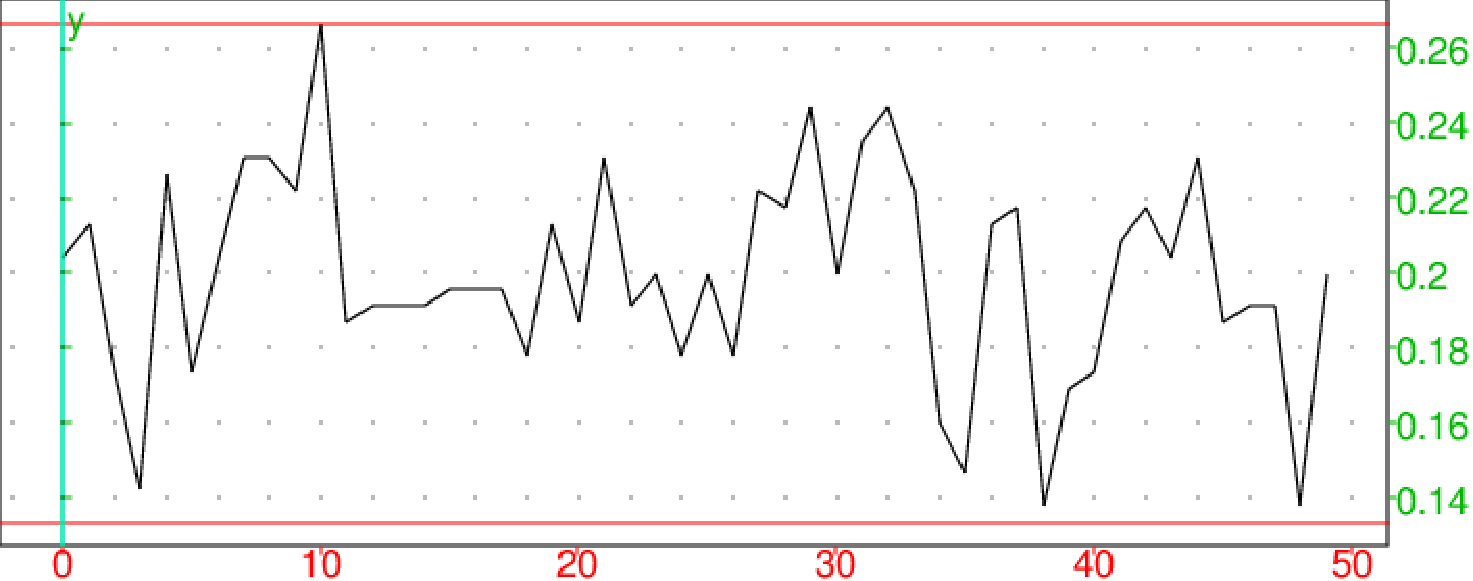
\includegraphics[width=\textwidth]{stattest}
 On analyse successivement $t$ échantillons de taille $n=225$ pour, 
$t\in {10, 20, 50, 100, 200, 500}$.
Pour notre problème, l’intervalle de fluctuation au seuil de 95\% est :
$p-\frac{1}{\sqrt n} p+\frac{1}{\sqrt n}$ avec $p=\frac{1}{5}$ et $n=225$ 
c'est \`a dire $\frac{2}{15},\frac{4}{15}$\\
Pour savoir si la simulation est corecte on fait un programme pour savoir si
on a bien dans 95\% des cas $p$ dans l'intervalle $\frac{2}{15},\frac{4}{15}$\\
On note {\tt N} le nombre de fois que l'on fait une simulation (une simulation
c'est 225 tirages).\\
Pour la {\tt k} i\`eme simulation, ({\tt k=1..N}) on note :\\
{\tt L} la liste des 225 tirages obtenus,\\
{\tt n} le nombre de fois que l'on a obtenu une boule verte,\\
{\tt p} le  pourcentage de boules vertes obtenues par cette simulation,\\l
{\tt s} le nombre de tirages tels que {\tt 2/15<p<4/15} lorsqu'on a fait 
{\tt k} simulations,\\
{\tt sn} le nombre de fois que l'on a obtenu une boule verte lorsqu'on a fait 
{\tt k} simulations.\\
{\tt pcn} le pourcentage de boules vertes obtenues  par ces {\tt N*225}
tirages est donc {\tt sn/(225*N)} 
Le nombre de fois o\`u on a {\tt 2/15<p<4/15} est {\tt s}. En pourcentage 
cela fait donc {\tt pc=s/N}.\\
On v\'erifie alors si {\tt pc>0.95}

\begin{verbatim}
test0(N):={
  local s,L,p,n,pc,sn,pcn,k,Le;
  s:=0;sn:=0;
Le:=NULL;
pour k de 1 jusque N faire
  L:=[randmultinomial([4/5,1/5],["R","V"])$(j=1..225)];
  n:=count_eq("V",L)
  p:=n/225;
  Le:=Le,p;
fpour;
 retourne Le;
  }:;
test(N):={
  local s,L,p,n,pc,sn,pcn,k,Le;
  s:=0;sn:=0;
Le:=NULL;
pour k de 1 jusque N faire
  L:=[randmultinomial([4/5,1/5],["R","V"])$(j=1..225)];
  n:=count_eq("V",L)
  p:=n/225;
  Le:=Le,p;
  si p>2/15 and p<4/15 alors s:=s+1; fsi;
  sn:=sn+n;
fpour;
  pc:=evalf(s/N);
  pcn:=evalf(sn/N/225);
  si pc>0.95 alors retourne pcn,pc,"correcte"; sinon retourne pcn,pc,"pas correcte"; fsi;
  }:;
\end{verbatim}
On tape :\\
{\tt test(10)}\\
On obtient :\\
{\tt 0.203111111111,1.0,"correcte"}\\
On tape :\\
{\tt test(20)}\\
On obtient :\\
{\tt 0.194888888889,0.95,"pas correcte"}\\
On tape :\\
{\tt test(50)}\\
On obtient :\\
{\tt 0.194311111111,0.98,"correcte"}\\
On tape :\\
{\tt test(100)}\\
On obtient :\\
{\tt 0.198888888889,0.97,"correcte"}\\
On tape :\\
{\tt test(200)}\\
On obtient :\\
{\tt 0.193777777778,0.99,"correcte"}\\
{\tt test(500)}\\
On obtient :\\
{\tt 0.19984,0.984,"correcte"}\\
On tape :\\
{\tt plotlist([10,20,50,100,200,500],[0.203,0.195,0.194,0.199,0.1940.1999] ),
droite(y=0.2)}\\
On obtient :\\
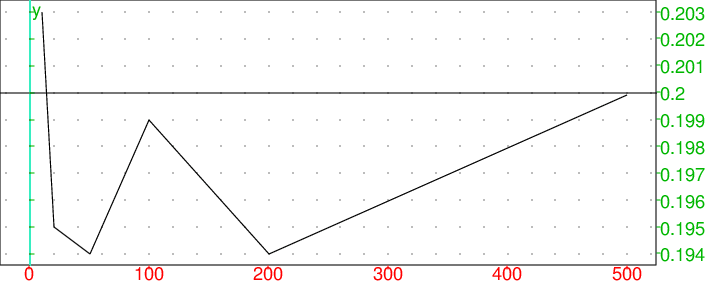
\includegraphics[width=\textwidth]{statconv}
\subsection{Tirage selon une loi normale : {\tt randnorm randNorm}}\index{randnorm}\index{randNorm}
\noindent {\tt randnorm(m,sigma)} ou {\tt randNorm(m,sigma)} renvoie au hasard 
des nombres r\'epartis selon la loi normale de moyenne {\tt  m} et d'\'ecart 
type {\tt sigma}.\\
On tape :
\begin{center}{\tt randnorm(0,1)}\end{center}
On obtient par exemple :
\begin{center}{\tt 0.549605372982}\end{center}
ou on obtient par exemple :
\begin{center}{\tt  -0.58946494465}\end{center}
On tape :
\begin{center}{\tt randnorm(2,1)}\end{center}
On obtient par exemple :
\begin{center}{\tt 2.54178274488}\end{center}
\subsection{Tirage selon une loi exponentielle : {\tt randexp}}\index{randexp}
\noindent {\tt randexp(a)} renvoie au hasard 
des nombres r\'epartis selon la loi exponentielle de param\`etre {\tt a}
positif.\\
La densit\'e de probabilit\'e est proportionnelle \`a $\exp(-a*t)$ et on a :\\
Proba($X\leq t$)=$a\int_0^t\exp(-a*u)du$.\\
On tape :
\begin{center}{\tt randexp(1)}\end{center}
On obtient par exemple :
\begin{center}{\tt 0.310153677284}\end{center}
ou on obtient par exemple :
\begin{center}{\tt 0.776007926195}\end{center}

\subsection{Matrice al\'eatoire : {\tt ranm randmatrix randMat}}\index{ranm}\index{randmatrix}\index{randMat}
{\tt ranm} (ou {\tt randmatrix} ou {\tt randMat}) peut avoir comme 1,2 ou 3 
arguments :\\
\begin{itemize}
\item avec un entier {\tt s} comme argument, {\tt ranm} renvoie 
une liste de longueur {\tt s} dont les \'el\'ements sont des entiers pris au 
hasard de fa\c{c}on \'equiprobable dans :\\
 {\tt [-99,-98,...,98,99]}.\\
On tape :
\begin{center}{\tt ranm(5)}\end{center}
On obtient par exemple :
\begin{center}{\tt [-40,27,4,-1,94]}\end{center}

\item avec deux entiers {\tt n,p} comme argument, {\tt ranm} renvoie une 
matrice de {\tt n} lignes et {\tt p} colonnes dont les \'el\'ements sont des 
entiers pris au hasard de fa\c{c}on \'equiprobable dans :\\
 {\tt [-99,-98,...,98,99]}.\\
On tape :
\begin{center}{\tt ranm(2,3)}\end{center}
On obtient par exemple :
\begin{center}{\tt [[-32,53,-44],[10,-4,25]]}\end{center}

\item avec deux entiers {\tt n,p} et un entier relatif {\tt a} comme argument, 
{\tt ranm} renvoie une matrice de {\tt n} lignes et {\tt p} colonnes dont 
les \'el\'ements sont des entiers pris au hasard de fa\c{c}on \'equiprobable 
dans  {\tt [0;a[} (ou {\tt ]a;0]} si {\tt a} est n\'egatif)\\
On tape :
\begin{center}{\tt ranm(2,3,10)}\end{center}
On obtient par exemple :
\begin{center}{\tt[[8,3,7],[7,9,1]]}\end{center}
\item avec deux entiers {\tt n,p} et un intervalle {\tt a..b} comme argument, 
{\tt ranm} renvoie une matrice de {\tt n} lignes et {\tt p} colonnes dont les 
\'el\'ements sont des r\'eels  pris au hasard de fa\c{c}on \'equiprobable dans 
{\tt [a;b[}.\\
On tape :
\begin{center}{\tt ranm(2,3,0..1)}\end{center}
On obtient par exemple :
\begin{center}{\tt [[0.840187716763,0.394382926635,0.783099223394],}\end{center}
\begin{center}{\tt [0.798440033104,0.911647357512,0.197551369201]] }\end{center}
\item deux entiers {\tt n,p} et une fonction al\'eatoire  de {\tt Xcas} qu'il 
faut quoter, dans ce cas 
{\tt ranm} renvoie une matrice de {\tt n} lignes et {\tt p} colonnes dont 
les \'el\'ements sont pris au hasard selon la fonction donn\'ee en 
troisi\`eme argument.\\ 
On tape :
\begin{center}{\tt ranm(3,2,'rand(3)')}\end{center}
ou
\begin{center}{\tt ranm(3,2,3)}\end{center}
On obtient par exemple :
\begin{center}{\tt [[2,1],[0,0],[1,0]]}\end{center}
On tape :
\begin{center}{\tt ranm(1,2,'randnorm(0,1)')}\end{center}
On obtient par exemple :
\begin{center}{\tt [[1.37439065645,-1.33195982697]]}\end{center}
\end{itemize}

 
\section{D\'eplacement al\'eatoire}
\subsection{D\'eplacement sur un axe}
%Tous les programmes de cette section se trouvent dans le fichier {\tt deplacement}.\\
Une tortue se d\'eplace sur un axe gradu\'e.\\
Au d\'ebut de chaque parcours la tortue se trouve \`a l'origine.\\
On choisit de la faire avancer en jouant \`a pile ou face :
pile la tortue reste sur place,
face elle avance d'une unit\'e.\\ 
Un parcours al\'eatoire de la tortue est constitu\'e par 5 tirages al\'eatoires.\\
On veut simuler 30 parcours al\'eatoires et trouver la 
probabilit\'e de l'\'ev\'enement : la tortue est arriv\'ee  au point d'abscisse
 $x_i$ pour $x_i \ \in \mathbb{N}$.
\subsubsection{Simulation d'un parcours}\label{sec:deplaxe}
On note {\tt T} l'abscisse du point d'arriv\'ee de la tortue.\\
On \'ecrit le programme {\tt parcours}, en utilisant {\tt rand(2)} qui renvoie 
de fa\c{c}on \'equiprobable 0 ou 1.\\
On consid\`ere que 0 correspond \`a pile et correspond 1 \`a face.
\begin{verbatim}
parcours() :={
  local T,r;
  T:=0;
  // on fait 5 tirages
  for (k:=1;k<6;k++){ 
    r:=rand(2);
    // la tortue avance si r==1 (tirage = face)
    if (r==1){
       T:=T+1;
    }
  }
  return(T);
}; 
\end{verbatim} 
Voici les r\'esultats obtenus lorsque l'on fait  10 fois 
{\tt parcours()} ,on tape:\\
{\tt for (k:=1;k<11;k++){ parcours()}}\\
On obtient par exemple :\\
{\tt 4,2,4,1,1,4,3,2,2,1}

\subsubsection{Simulation de n  parcours}
On note {\tt T} l'abscisse du point d'arriv\'ee de la tortue et 
{\tt TA} le tableau des r\'esultats : {\tt TA[0]} represente le nombre de fois 
que la tortue est au point {\tt 0} \`a l'arriv\'ee.\\
On \'ecrit  le programme suivant  dans l'\'editeur de programmes de {\tt Xcas} 
(raccourci {\tt Alt+p})
et on sauve ce programme dans le fichier {\tt parsim}.
\begin{verbatim}
parcoursim(n) :={
  local T,r,TA,R,j,k;
  ClrGraph();
  TA:=[0,0,0,0,0,0];
  for (j:=1;j<n+1;j++){
    T:=0;
    for (k:=1;k<6;k++){ 
      r:=rand(2);
      if (r==1){
        T:=T+1;
      }
    }
  TA[T]:=TA[T]+1;
  };
  orint(TA);
  switch_axes(NULL);
  xyztrange(-0.5,5.2,-0.1,16.0,-10.0,10.0,-10.0,-10.0,
            -0.5,5.2,-0.1,16.0,1);
  R:=segment(0,i*TA[0]);	
  R:=R,segment(1,1+i*TA[1]);
  R:=R,segment(2,2+i*TA[2]);
  R:=R,segment(3,3+i*TA[3]);
  R:=R,segment(4,4+i*TA[4]);
  R:=R,segment(5,5+i*TA[5]);
  return R;
}; 
\end{verbatim} 
{\bf Attention}
Ici {\tt parcoursim} renvoie une liste de  segments et \'ecrit en bleu la valeur de {\tt TA}.
Le programme se trouve dans un  \'editeur {\tt prg} de {\tt Xcas}, on le teste
avec  le bouton {\tt OK}, puis si on a obtenu {\tt  //Success compilling}, 
le programme est valid\'e.\\
On tape dans la ligne de commande :\\
{\tt parcoursim(30)}\\
On obtient en bleu :\\
{\tt TA:[0,4,14,6,6,0]}\\
et le graphique :\\

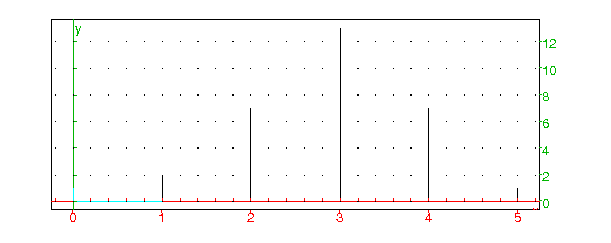
\includegraphics[width=\textwidth]{parsim}

Voici des r\'esultats obtenus pour la liste des abscisses des points 
d'arriv\'ee :\\
pour {\tt parcoursim(30)} on a trouv\'e {\tt [0,2,7,13,7,1]}\\
pour {\tt parcoursim(300)} on a trouv\'e {\tt [7,41,94,102,47,9]}\\
pour {\tt parcoursim(1000)} on a trouv\'e {\tt [36,172,310,306,148,28]}\\
pour {\tt parcoursim(10000)} on a trouv\'e {\tt [287,1575,3184,3136,1517,301]}
\subsubsection{Analyse des r\'esultats}
%Soit l'espace probabilis\'e ($\Omega, \thau, Prob$)\\
Soit l'univers $\Omega$ form\'e par les 5 tirages successifs possibles (chacun 
\'etant \'equiprobable) :\\
$\Omega=\{\{p,p,p,p,p\},\{p,p,p,p,f\},\{p,p,p,f,p\},...,\{f,f,f,f,f,\}\}$.\\
$\Omega$ a $2^5=32$ \'el\'ements.\\
Soit {\tt A} la variable al\'eatoire \'egale \`a l'abscisse du point d'arriv\'ee.\\
On  a :\\
$\displaystyle {\tt P(A=0)=\frac{1}{2^5}=0.03125}$ car cela correspond \`a 5 fois "pile",\\
$\displaystyle {\tt P(A=1)=\frac{5}{2^5}=0.15625}$ car cela correspond \`a 4 fois "pile" et 1 
fois "face" ce qui peut se produire de 5 fa\c{c}ons, \\
$\displaystyle {\tt P(A=2)=\frac{10}{2^5}= 0.3125}$ car cela correspond \`a 3 fois "pile" et 2 
fois "face" ce qui peut se produire de $C_5^2=$ 10 fa\c{c}ons, \\
$\displaystyle {\tt P(A=3)=\frac{10}{2^5}= 0.3125}$ car cela correspond \`a 2 fois "pile" et 3 
fois "face" ce qui peut se produire de $C_5^3=$ 10 fa\c{c}ons, \\
$\displaystyle {\tt P(A=4)=\frac{5}{2^5}=0.15625}$ car cela correspond \`a 1 fois "pile" et 4
fois "face" ce qui peut se produire de 5 fa\c{c}ons, \\
$\displaystyle {\tt P(A=5)=\frac{1}{2^5}=0.03125}$ car cela correspond \`a 5 fois "face".
\subsection{D\'eplacement dans deux directions}
Au d\'ebut de chaque parcours la tortue se trouve \`a l'origine.\\
On choisit de la faire avancer en jouant \`a pile ou face :\\
- pile, la tortue avance d'une unit\'e selon un axe vertical,\\
- face, elle avance d'une unit\'e selon un axe horizontal.\\ 
Un parcours al\'eatoire de la tortue est constitu\'e par 5 tirages al\'eatoires.\\
On veut simuler {\tt n} parcours al\'eatoires et trouver la 
probabilit\'e de l'\'ev\`enement : le parcours al\'eatoire de la tortue se termine au point de coordonn\'ees $[x,y]$ pour $(x,y) \ \in N \times N$
\subsubsection{Simulation d'un parcours}
On note {\tt X,Y} les coordonn\'ees du point d'arriv\'ee de la tortue.\\
On \'ecrit :
\begin{verbatim}
parcours2() :={
  local X,Y,r;
  X:=0;
  Y:=0;
  for (k:=1;k<6;k++){
    r:=rand(2);
    if (r==1){
       X:=X+1;
    } else {
       Y:=Y+1;
    }
  }
  return([X,Y]);
}; 
\end{verbatim} 
Voici les r\'esultats obtenus lorsque l'on fait 10 fois {\tt parcours2()} :\\
{\tt [2,3],[1,4],[3,2],[4,1],[3,2],[2,3],[1,4],}\\
{\tt [1,4],[3,2],[2,3]}\\
On remarque qu'\`a chaque tirage soit {\tt X}, soit {\tt Y} est augment\'e 
d'une unit\'e donc \`a chaque tirage {\tt X+Y} aygmente de 1. Au d\'ebut 
{\tt X+Y=0}, donc, 
au bout de 5 tirages c'est \`a dire \`a la derni\`ere \'etape {\tt X+Y=5}.\\
Il suffit donc de connaitre l'abscisse d'arriv\'ee {\tt X} pour connaitre le 
point d'arriv\'ee ({\tt point(X,5-X))}). Ce probl\`eme est donc le m\^eme que 
le pr\'ec\'edent.
\subsubsection{Simulation de n  parcours}
On note {\tt XA} le tableau des r\'esultats selon les abscisses.\\ 
On remarquera qu'ici {\tt Y} ne sert \`a rien puisqu'on peut rep\'erer le 
point d'arriv\'ee seulement \`a l'aide de son abscisse, elle permet juste de 
visualiser le point d'arriv\'ee.\\
On \'ecrit :
\begin{verbatim}
parcoursim2(n) :={
  local X,Y,r,j,k,XA;
  XA:=[0,0,0,0,0,0];
  for (j:=1;j<n+1;j++){
    r:=rand(2);
    X:=0;
    Y:=0;
    for (k:=1;k<6;k++){
      if (r==1){
        X:=X+1;
      } else {
        Y:=Y+1;
      }
    r:=rand(2);
    }
  XA[X]:=XA[X]+1;
  }
  switch_axes(NULL);
  ClrGraph();
  xyztrange(-0.5,5.2,-0.1,16.0,-10.0,10.0,-10.0,-10.0,
            -0.5,5.2,-0.1,16.0,1);
 
  return([XA,segment(0,i*XA[0]),segment(1,1+i*XA[1]),
     segment(2,2+i*XA[2]),segment(3,3+i*XA[3]),
     segment(4,4+i*XA[4]),segment(5,5+i*XA[5])]);
}; 
\end{verbatim} 
Voici les r\'esultats obtenus :\\
pour {\tt parcoursim2(30)} on a trouv\'e :\\
{\tt XA=[0,4,9,9,7,1]}\\
pour {\tt parcoursim2(300)} on a trouv\'e :\\
{\tt XA=[6,48,91,99,46,10]}\\
pour {\tt parcoursim2(1000)} on a trouv\'e :\\
{\tt XA=[26,170,313,320,148,23]}\\
pour {\tt parcoursim2(10000)} on a trouv\'e :\\
{\tt XA=[290,1498,3207,3128,1572,305]}\\
{\bf Attention}
Ici {\tt parcoursim2} renvoie une liste de segments  : ces segments seront 
donc dessin\'es dans un \'ecran de g\'eom\'etrie et dans l'\'ecran {\tt DispG}.
Il faut donc \'ecrire {\tt ClrGraph()} en d\'ebut de 
programme si on veut effacer l'\'ecran de g\'eom\'etrie {\tt DispG}.
\subsubsection{Analyse des r\'esultats}
On a donc la m\^eme analyse que dans le parcours lin\'eaire. \\
Soit {\tt A} la variable al\'eatoire \'egale aux coordonn\'ees du point d'arriv\'ee.\\
$\displaystyle {\tt P(A=[0,5])=\frac{1}{2^5}= 0.03125}$ car cela correspond \`a 5 fois "pile",\\
$\displaystyle {\tt P(A=[1,4])=\frac{5}{2^5}=0.15625}$ car cela correspond \`a 4 fois "pile" et 1 
fois "face" ce qui peut se produire de 5 fa\c{c}ons, \\
$\displaystyle {\tt P(A=[2,3])=\frac{10}{2^5}=0.3125}$ car cela correspond \`a 3 fois "pile" et 2 
fois "face" ce qui peut se produire de $C_5^2=$ 10 fa\c{c}ons, \\
$\displaystyle {\tt P(A=[3,2])=\frac{10}{2^5}= 0.3125}$ car cela correspond \`a 2 fois "pile" et 3 
fois "face" ce qui peut se produire de $C_5^3=$ 10 fa\c{c}ons, \\
$\displaystyle {\tt P(A=[4,1])=\frac{5}{2^5}=0.15625}$ car cela correspond \`a 1 fois "pile" et 4
fois "face" ce qui peut se produire de 5 fa\c{c}ons, \\
$\displaystyle {\tt P(A=[5,0])=\frac{1}{2^5}= 0.03125}$ car cela correspond \`a 5 fois "face".
\section{Les trois cartes bicolores}
On met dans un chapeau trois cartes : une des cartes a deux c\^ot\'es rouges,
 une autre a un c\^ot\'e rouge et un c\^ot\'e blanc et la troisi\`eme a deux
 c\^ot\'es blancs.\\
On tire une carte : le c\^ot\'e que nous voyons est rouge.\\
Quelle est la probabilit\'e pour que l'autre c\^ot\'e soit blanc ?   
\subsection{Simulation de n tirages}
Pour \'ecrire le programme de simulation,
on num\'erote les cartes par 0,1 et 2 et on num\'erote les faces de chaque 
carte par 0 et 1 : par exemple la carte blanche a le num\'ero {\tt 0},
la carte bicolore a le num\'ero {\tt 1}, la carte rouge a le num\'ero {\tt 2}
 et la face blanche de la carte bicolore a le num\'ero {\tt 0}.\\
Puis, on repr\'esente donc une carte par un vecteur qui est la couleur de ses 
faces :\\
 par exemple la carte bicolore sera repr\'esent\'ee par {\tt [B,R]}.\\
On peut aussi repr\'esenter le blanc par 0 et le rouge par 1 : \\
par exemple la carte bicolore sera repr\'esent\'ee par {\tt [0,1]}.\\
On repr\'esente ainsi les cartes par un vecteur de deux composantes 0 ou 1 
(0 et 1 d\'esigne la couleur).\\
La variable {\tt C:=[[0,0],[0,1],[1,1]]} repr\'esente donc les trois cartes :\\
{\tt [0,0]} est la carte avec 2 faces blanches, {\tt [1,1]} est la carte 
avec 2 faces rouges et {\tt [0,1]} est la carte bicolore (on a suppos\'e que 
la face blanche a le num\'ero 0 et la rouge le num\'ero 1).\\ 
{\tt C} est donc une matrice et la valeur de {\tt C[a,b]} (pour  {\tt a=0,1,2} 
et {\tt b=0,1)} repr\'esente la couleur de la face {\tt b} de la carte {\tt a}.\\
On tire une des cartes ({\tt a:=rand(3);}),\\
 puis on tire la face visible ({\tt b:=rand(2);}).\\
 Si {\tt b} est la face visible, {\tt irem(b+1,2)} c'est
\`a dire {\tt b+1 mod 2} est la face cach\'ee.\\
On simule $n$ tirages qui donne comme cot\'e visible une face rouge et on 
compte le nombre de cartes bicolores.\\
On \'ecrit pour cela le programme {\tt cartebicolor} :
\begin{verbatim}
cartebicolor(n):={
local C,a,b,nbi;
C:=[[0,0],[0,1],[1,1]];
//nbi est le nbre de cartes bicolores obtenus 
//qd la face visible est blanche
nbi:=0
for (k:=0;k<n;k++){
//on tire une carte
a:=rand(3);
// on tire une face (la face visible)
b:=rand(2);
// on refait le tirage si la face visible est blanche
while (C[a,b]==0) {
a:=rand(3);
b:=rand(2);
}
//la face visible est rouge, si la face cachee est blanche,
// nbi augmente de 1
if (C[a,irem(b+1, 2)]]==0) {
nbi:=nbi+1;
}
}
return(evalf(nbi/n));
};
\end{verbatim} 
On a obtenu :\\
{\tt cartebicolor(300)=0.34}\\ 
{\tt cartebicolor(3000)=0.343666666667}\\
{\tt cartebicolor(30000)=0.331533333333}
\subsection{Analyse du r\'esultat}
Etant donn\'e qu'il y a autant de c\^ot\'es rouges que de c\^ot\'es  blancs, 
le probl\`eme suivant a la m\^eme r\'eponse :\\
On tire une carte : le c\^ot\'e que nous voyons est blanc.\\
Quelle est la probabilit\'e pour que l'autre c\^ot\'e soit rouge ?\\
ou encore :\\
On tire une carte : nous voyons un c\^ot\'e de cette carte.\\
Quelle est la probabilit\'e pour que l'autre c\^ot\'e ne soit pas de la 
m\^eme couleur?\\   
Cela revient \`a demander quelle est la probabilit\'e pour que l'on ait tir\'e
la carte bicolore. Comme il y a trois cartes dont une seule est bicolore,
 la probabilit\'e cherch\'ee est \'egale \`a $\frac{1}{3}$.\\  
On peut aussi traiter ce probl\`eme avec les probabilit\'es conditionnelles :\\
soit $\Omega$ l'ensemble des faces visibles. On rep\'ere la face visible par
 2 nombres le num\'ero de sa carte et son num\'ero de face (par exemple [1,0] 
d\'esigne la face 0 de la carte 1 alors que  [0,1] 
d\'esigne la face 1 de la carte 0) on a \\
 $\Omega=\{[0,0],[0,1],[1,0],[1,1],[2,0],[2,1]\}$.\\ 
Les trois premiers \'el\'ements de $\Omega$ ont comme face visible une face
blanche, les trois derniers \'el\'ements de $\Omega$ sont comme face visible 
une face rouge.\\
Soit A l'\'ev\`enement "le cot\'e visible est rouge",\\
soit B l'\'ev\`enement "le cot\'e non visible est blanc",\\
soit C l'\'ev\`enement "le cot\'e visible est rouge et le cot\'e non visible 
est blanc" ou "le cot\'e visible est blanc et le cot\'e non visible est rouge"
 (ie la carte tir\'ee est bicolore).\\
P(A)=$\displaystyle \frac{1}{2}$\\
P(B)=$\displaystyle \frac{1}{2}$\\
P(C)=$\displaystyle \frac{1}{3}$\\
P(A et B)=$\displaystyle \frac{1}{6}$\\
P(C)=P(A et B)+P(nonA et nonB)=$\displaystyle \frac{1}{3}$\\
P(B/A)=P(A et B)/P(A)=$\displaystyle \frac{1}{6}$/$\displaystyle \frac{1}{2}$=
$\displaystyle \frac{1}{3}$\\
On peut aussi num\'eroter les faces rouges et les faces blanches et dire qu'un 
couple represente une carte et le premier \'el\'ement du couple est la face 
visible.\\
Par exemple, $(R_3,B_3)$ repr\'esente la carte bicolore ayant comme face
 visible la face rouge.\\
$\Omega=\{(R_1,R_2),(R_2,R_1),(R_3,B_3),(B_3,R_3),(B_1,B_2),(B_2,B_1)\}$.\\
Soit A l'\'ev\`enement "le cot\'e visible est rouge" :\\
A=$\{(R_1,R_2),(R_2,R_1),(R_3,B_3)\}$\\
Donc :\\
P(A)=$\displaystyle \frac{1}{2}$\\
soit B l'\'ev\`enement "le cot\'e non visible est blanc" :\\
A et B=$\{(R_3,B_3)\}$\\
Donc :\\
P(A et B)=$\displaystyle \frac{1}{6}$\\
Donc :\\
P(B/A)=P(A et B)/P(A)=$\displaystyle \frac{1}{6}/ \frac{1}{2}$=
$\displaystyle \frac{1}{3}$\\
\section{Les quatre cartes bicolores}
On met dans un chapeau quatre cartes : une des cartes a deux c\^ot\'es blancs,
 une autre a un c\^ot\'e rouge et un c\^ot\'e blanc et les deux restantes ont
 deux c\^ot\'es rouges.\\
On tire une carte : le c\^ot\'e que nous voyons est rouge.\\
Quelle est la probabilit\'e pour que l'autre c\^ot\'e soit blanc ?   
\subsection{Simulation}
\begin{verbatim}
cartebic4(n):={
  local C,a,b,nbi;
  C:=[[0,0],[0,1],[1,1],[1,1]];
  nbi:=0
  for (k:=0;k<n;k++){
    a:=rand(4);
    b:=rand(2);
    while (C[a,b]==0) {
      a:=rand(4);
      b:=rand(2);
    }
    if (C[a,irem(b+1, 2)]==0) {
      nbi:=nbi+1;
    }
  }
  return(evalf(nbi/n));
};
\end{verbatim} 
On a obtenu :\\
{\tt cartebic4(300)= 0.18}\\ 
{\tt cartebic4(3000)= 0.203666666667}\\
{\tt cartebic4(30000)=0.2019}
\subsection{Analyse du r\'esultat}
On va traiter ce probl\`eme avec les probabilit\'es conditionnelles :\\
soit $\Omega$ l'ensemble des faces visibles. \\
On  rep\'ere la face visible par 
2 nombres le num\'ero de sa carte et son num\'ero de face (par exemple [1,0] 
d\'esigne la face 0 de la carte 1  alors que  
[0,1] d\'esigne la face 1 de la carte 0) on a \\
 $\Omega=\{[0,0],[0,1],[1,0],[1,1],[2,0],[2,1],[3,0],,[3,1]\}$.\\ 
Onsuppose que la carte 0 a 2 faces blanches,que la face 0 de la carte 1 est
blanche et que sa face 1 est rouge et que les cartes 2 et 3 ont 2 faces rouges.
Donc les trois premiers \'el\'ements de $\Omega$ sont des faces blanches, les 
cinq derniers \'el\'ements de $\Omega$ sont des faces rouges.\\
Soit A l'\'ev\`enement "le cot\'e visible est rouge",\\
soit B l'\'ev\`enement "le cot\'e non visible est blanc",\\
soit C l'\'ev\`enement la carte tir\'ee est bicolore.\\
P(A)=$\displaystyle \frac{5}{8}$\\
P(B)=$\displaystyle \frac{3}{8}$ \\  
P(A et B)=$\displaystyle \frac{1}{8}$\\
P(C)=P(A et B)+P(nonA et nonB)=$\displaystyle \frac{1}{4}$\\
P(B/A)=P(A et B)/P(A)=$\displaystyle \frac{1}{8}$/$\displaystyle \frac{5}{8}$=$\displaystyle \frac{1}{5}$.\\
Donc la probabilit\'e que la face cach\'ee soit blanche sachant que la face 
visible est rouge est :
 $\displaystyle\frac{1}{5}$\\
Etant donn\'e qu'il n'y a pas autant de c\^ot\'es rouges que de c\^ot\'es  
blancs, le probl\`eme pos\'e n'est pas le m\^eme que :\\
On tire une carte : le c\^ot\'e que nous voyons est blanc.\\
Quelle est la probabilit\'e pour que l'autre c\^ot\'e soit rouge ?\\
On a :\\
P(nonA)=$\displaystyle \frac{3}{8}$\\   
P(nonB)=$\displaystyle \frac{5}{8}$\\ 
P(nonA et nonB)=$\displaystyle \frac{1}{8}$\\
P(nonB/nonA)=P(nonA et nonB)/P(nonA)=$\displaystyle \frac{\frac{1}{8}}{\frac{3}{8}}$= $\displaystyle \frac{1}{3}$.\\
On retrouve la m\^eme probabilit\'e que dans le cas des trois cartes 
bicolores car la probabilit\'e demand\'ee  ne tient compte que de l'ensemble 
des cartes qui ont un c\^ot\'e 
blanc et dans les deux probl\`emes cet ensemble est le m\^eme.\\
ce n'est pas non plus  le m\^eme probl\`eme que :\\
On tire une carte : nous voyons un c\^ot\'e de cette carte.\\
Quelle est la probabilit\'e pour que l'autre c\^ot\'e ne soit pas de la 
m\^eme couleur?\\
On demande ici la probabilit\'e de tirer la carte bicolore c'est \`a dire :
P(C)=$\displaystyle \frac{1}{4}$\\
{\bf Remarque}\\
P(C)=P(A)*P(B/A)+P(nonA)*P(nonB/nonA)=\\
P(A et B)+P(nonA et nonB)=
$\displaystyle \frac{1}{4}=\frac{3}{8}*\frac{1}{3}+\frac{5}{8}*\frac{1}{5}$
\section{La voiture et les deux ch\`evres}
Un candidat \`a un jeu doit choisir entre trois portes et gagne ce qui se trouve derri\`ere la porte choisie. Il y a une voiture derri\`ere une porte et une ch\`evre derri\`ere chacune des deux autres portes.
Le candidat choisit une porte et le pr\'esentateur qui connait la porte
 gagnante,  ouvre une des deux portes restantes derri\`ere laquelle se trouve
une ch\`evre, et demande au candidat si il veut changer son choix.
A votre avis le candidat a-t-il plus de chances de gagner la voiture en 
changeant  syst\'ematiquement son choix ?\\
Pour r\'epondre \`a cette question, commen\c{c}ons par une simulation.
\subsection{Simulation}
Le param\`etre {\tt n} repr\'esente le nombre de jeux.\\
{\tt ng1} est le nombre de fois o\`u le candidat gagne quand il ne change 
jamais de choix (situation1) et \\
{\tt ng2} est le nombre de fois o\`u le candidat gagne quand il change 
syst\'ematiquement de choix (situation2).\\
La porte o\`u l'on met la voiture est tir\'ee au hasard 
({\tt v:=rand(3);P[v]:=1}).\\
Le candidat choisit une porte au hasard ({\tt a:=rand(3)}).\\
Si {\tt (a==v)} il gagne dans la situation1 ({\tt ng1:=ng1+1}) et perd dans la 
situation2 ({\tt ng2} reste inchang\'e).\\
Si {\tt (a!=v)} il gagne dans la situation2 ({\tt ng2:=ng2+1}) et perd dans la 
situation1 ({\tt ng1} reste inchang\'e).\\
Dans ce qui suit la variable {\tt P} ne sert \`a rien et permet juste de 
visualiser les 3 portes (si  {\tt P[n]==0}, derri\`ere la porte de num\'ero 
{\tt  n} il y a une ch\`evre, et si {\tt P[n]==1}, derri\`ere la porte de 
num\'ero {\tt  n} il y a une voiture). \\
On \'ecrit le programme {\tt chevre} qui compte le nombre de gains dans
{\tt ng1} quand on ne change pas son choix et 
qui compte le nombre de gains dans
{\tt ng2} quand on change syst\'ematiquement son choix.
\begin{verbatim}
chevre(n):={
local a,v,ng1,ng2;
ng1:=0;
ng2:=0
for (k:=0;k<n;k++){
\\on choisit la porte v o\`u l'on met la voiture
v:=rand(3);
P:=[0,0,0];
P[v]:=1;
//le candidat choisit une porte a
a:=rand(3);
if (a==v){ng1:=ng1+1;}
else {ng2:=ng2+1;}
}
return ([evalf(ng1/n),evalf(ng2/n)]);
};
\end{verbatim} 
On a obtenu :
{\tt chevre(10000)= [0.3303,0.6697]}
\subsection{Analyse du r\'esultat}
La voiture est derri\`ere la porte {\tt v}.\\
Le candidat choisit une porte {\tt a} au hasard.\\
Si {\tt (a==v)} il gagne dans la situation1 et perd dans la situation2 et,\\
si {\tt (a!=v)} il gagne dans la situation2 et perd dans la situation1.\\
On a  donc :\\
P(a=v)=$\displaystyle \frac{1}{3}$\\  
et donc P(a!=v)=1-P(a=v)=$\displaystyle \frac{2}{3}$ \\
Le candidat a donc deux fois plus de chances de gagner s'il change son choix 
syst\'ematiquement !\\
{\bf Remarque} \\
Pourtant malgr\'e la simplicit\'e de la situation, notre intuition semble en 
d\'efaut ...\\
Si ce qui pr\'ec\'ede ne vous a pas convaincu faites le m\^eme probl\`eme avec
 100 portes (1 voiture et 99 ch\`evres) et le pr\'esentateur ouvre 98 portes 
derri\`ere lesquelles il y a des ch\`evres : on comprend bien qu'en d\'esignant
 une porte, la voiture a plus de chances (99 chances sur 100)
d'\^etre derri\`ere les portes restantes, et en ouvrant les 98 portes le 
pr\'esentateur \'elimine 98 ch\`evres et donc derri\`ere la porte restante il 
y a  99 chances sur 100 pour qu'il y ait la voiture.
\section{Comment couper des spaghettis en trois ?}
Voici l'\'enonc\'e d'un probl\`eme :\\
On coupe de fa\c{c}on al\'eatoire un spaghetti en trois morceaux. Quelle est
la probabilit\'e pour qu'avec les trois morceaux obtenus on puisse former un triangle ?
Comment peut-on simuler cette situation ou autrement dit que veut dire "on coupe de fa\c{c}on al\'eatoire un spaghetti en trois morceaux" ?\\
On suppose dans ce qui suit le spaghetti de longueur 1.
\begin{itemize}
\item Premi\`ere m\'ethode : on choisit au hasard deux points $x$ et $y$ de 
[0,1].
\item Deuxi\`eme m\'ethode : on choisit au hasard un point $x$ de [0,1], puis 
on choisit au hasard le point $y$ dans [0,$x$].
\item Troisi\`eme m\'ethode : on choisit au hasard un point $x$ de [0,1], puis 
on choisit au hasard l'un des segments [0,$x$] ou [$x$,1], puis on choisit 
au hasard le point $y$ dans le segment choisi.
\item Quatri\`eme m\'ethode : on choisit au hasard un point $x$ de [0,1], puis 
on choisit le plus grand des segments [0,$x$] ou [$x$,1], puis on choisit 
au hasard le point $y$ dans le segment choisi.
\end{itemize}
Ces diff\'erentes m\'ethodes conduisent-elles au m\^eme r\'esultat ?\\
Quelle est la m\'ethode qui donne la plus forte probabilit\'e ?\\
Pour r\'epondre \`a ces questions commen\c{c}ons par des simulations.\\
Pour cela, il faut savoir r\'epondre \`a la question : \`a quelles conditions 
trois segments de longueurs $a$, $b$ et  $c=1-a-b$ forment-ils un triangle ?\\
Une condition necessaire et suffisante est que :\\
 $a<b+c$ et $b-c<a$ et $c-b<a$ ou encore que : \\
$a<1-a$ et $a+2b-1<a$ et $1-a-2b<a$ ou encore que : \\
$a<0.5$ et $b<0.5$ et $0.5<a+b$
\subsection{Simulation premi\`ere m\'ethode}
On choisit au hasard deux points d'abscisses $x$ et $y$ de l'intervalle [0;1].\\
On note :\\
{\tt x} et {\tt y} les abscisses des points de coupures.\\
{\tt a} et {\tt b} la longueur du premier et du deuxi\`eme morceau 
de spaghetti.\\
{\tt t} le nombre de triangles obtenus au bout de {\tt n} essais.
\begin{verbatim}
spag1(n):={
  local x,y,a,b,t;
  t:=0;
  for (k:=1;k<=n;k++){
     x:=evalf(rand(2^30)/2^30);
     y:=evalf(rand(2^30)/2^30);
     if (x<y) {
        a:=x;
        b:=y-x;
     } else {
        a:=y;
        b:=x-y;
     }
     if ((a<0.5) and (b<0.5) and (a+b>0.5)) {
        t:=t+1;
     }
  }
  return(evalf(t/n));
}; 
\end{verbatim} 
On a trouv\'e pour n=30000 :
{\tt 0.2506}\\ 
On a trouv\'e pour n=300000 :
{\tt 0.24965}
\subsection{Simulation deuxi\`eme m\'ethode}
On choisit au hasard un point d'abscisse $x$ de l'intervalle [0;1], puis
on choisit au hasard un point d'abscisse $y$ de l'intervalle $[0;x]$.\\
On note :\\
{\tt x} et {\tt y} les abscisses des points de coupures.\\
{\tt a} et {\tt b} la longueur du premier et du deuxi\`eme morceau 
de spaghetti.\\
{\tt t} le nombre de triangles obtenus au bout de {\tt n} essais.
\begin{verbatim}
spag2(n):={
  local x,y,a,b,t;
  t:=0;
  for (k:=1;k<=n;k++){
     x:=evalf(rand(2^30)/2^30);
     y:=evalf(rand(2^30)/2^30)*x;
     a:=y;
     b:=x-y;
     if ((a<0.5) and (b<0.5) and (a+b>0.5)) {
        t:=t+1;
     }
  }
  return(evalf(t/n));
}; 
\end{verbatim}
On a trouv\'e pour n=30000 :
{\tt 0.193266666667}\\
On a trouv\'e pour n=300000 :
{\tt 0.191666666667}
\subsection{Simulation troisi\`eme m\'ethode}
On choisit au hasard un point d'abscisse $x$ de l'intervalle [0;1], puis
on choisit au hasard l'intervalle $[0;x]$ ou $[x;1]$ 
puis, on choisit au hasard un point d'abscisse $y$ dans l'intervalle choisi.\\
On note :\\
{\tt x} et {\tt y} les abscisses des points de coupures.\\
{\tt a} et {\tt b} la longueur du premier et du deuxi\`eme morceau 
de spaghetti.\\
{\tt t} le nombre de triangles obtenus au bout de {\tt n} essais.
\begin{verbatim}
spag3(n):={
  local x,y,a,b,t;
  t:=0;
  for (k:=1;k<=n;k++){
     x:=evalf(rand(2^30)/2^30);
     if (rand(2)==0){
       y:=evalf(rand(2^30)/2^30)*x;
       a:=y;
       b:=x-y;
     } else {
       y:=evalf(rand(2^30)/2^30)*(1-x)+x;
       a:=x;
       b:=y-x;
     }
     if ((a<0.5) and (b<0.5) and (a+b>0.5)) {
       t:=t+1;
     }
  }
  return(evalf(t/n));
}; 
\end{verbatim}
On a trouv\'e pour n=30000 :
{\tt 0.195533333333}\\
On a trouv\'e pour n=300000 :
{\tt 0.194083333333}
\subsection{Simulation quatri\`eme m\'ethode}
On choisit au hasard un point d'abscisse $x$ de l'intervalle [0;1], puis
on choisit le plus grand des deux intervalles $[0;x]$ ou $[x;1]$ 
puis, on choisit au hasard un point d'abscisse $y$ dans l'intervalle choisi.\\
On note :\\
{\tt x} et {\tt y} les abscisses des points de coupures.\\
{\tt a} et {\tt b} la longueur du premier et du deuxi\`eme morceau 
de spaghetti.\\
{\tt t} le nombre de triangles obtenus au bout de {\tt n} essais.
\begin{verbatim}
spag4(n):={
  local x,y,a,b,t;
  t:=0;
  for (k:=1;k<=n;k++){
     x:=evalf(rand(2^30)/2^30);
     if (x>0.5){
       y:=evalf(rand(2^30)/2^30)*x;
       a:=y;
       b:=x-y;
     } else {
       y:=evalf(rand(2^30)/2^30)*(1-x)+x;
       a:=x;
       b:=y-x;
     }
     if ((a<0.5) and (b<0.5) and (a+b>0.5)) {
       t:=t+1;
     }
  }
  return(evalf(t/n));
}; 
\end{verbatim}
On a trouv\'e pour n=30000 :
{\tt 0.388366666667}\\
On a trouv\'e pour n=300000 :
{\tt 0.385946666667}\\

On remarque que :\\
0.194083333333*2 = 0.388166666666\\
 0.191666666667*2 = 0.383333333334\\
ln(2)-0.5= 0.19314718056\\
\subsection{Analyse des r\'esultats}
\subsubsection{Premi\`ere m\'ethode}
 Premi\`ere m\'ethode :  on choisit au hasard deux points $x$ et $y$ de [0,1].\\
On sait que si l'on obtient $x<0.5$, pour obtenir un triangle dans ce cas, 
il faut choisir $y$ dans l'intervalle 
$[\frac{1}{2},x+\frac{1}{2}]$ qui est un intervalle de longueur $x$. La probabilit\'e d'obtenir
un $y$ qui convient est donc alors \'egale \`a $x$.\\
On sait que si l'on obtient $x>0.5$, pour obtenir un triangle dans ce cas, 
il faut choisir $y$ dans l'intervalle 
$[x-\frac{1}{2},\frac{1}{2}]$ qui est un intervalle de longueur $1-x$. La probabilit\'e 
d'obtenir un $y$ qui convient est donc alors \'egale \`a $1-x$.\\
Donc la probabilit\'e d'obtenir un triangle est :\\
$\displaystyle \int_0^{\frac{1}{2}}xdx+\int_{\frac{1}{2}}^1(1-x)dx=\frac{1}{8}+\frac{1}{8}=\frac{1}{4}$
\subsubsection{Deuxi\`eme m\'ethode}
Deuxi\`eme m\'ethode : on choisit au hasard un point $x$ de [0,1], puis 
on choisit au hasard le point $y$ dans [0,$x$].\\
On sait que si l'on obtient $x<0.5$,
 on a une probabilit\'e nulle d'obtenir un triangle puisque ensuite on choisit 
$y$ v\'erifiant $y<x$.
On sait que si l'on obtient $x>0.5$,  pour obtenir un triangle dans ce cas, il
 faut choisir $y$ dans l'intervalle 
$[x-\frac{1}{2},\frac{1}{2}]$ qui est un intervalle de longueur $1-x$. La probabilit\'e 
d'obtenir un $y$ qui convient est donc \'egale \`a $\frac{1-x}{x}$.\\
Donc la probabilit\'e d'obtenir un triangle est :\\
$\displaystyle \int_{\frac{1}{2}}^1\frac{1-x}{x}dx=\ln(2)-\frac{1}{2}$
\subsubsection{Troisi\`eme m\'ethode}
Troisi\`eme m\'ethode : on choisit au hasard un point $x$ de [0,1], puis 
on choisit au hasard l'un des segments [0,$x$] ou [$x$,1], puis on choisit 
au hasard le point $y$ dans le segment choisi.\\
Si on choisit avec une probabilit\'e 0.5 l'un des deux segments $[0,x[$ ou
$[x,1[$, si $x<0.5$ pour obtenir un $y$ qui convient il faut choisir  (
avec une probabilit\'e de 0.5) 
l'intervalle  $[x,1[$ (qui est un intervalle de longueur $1-x$), puis choisir $y$ dans l'intervalle 
$[\frac{1}{2},x+\frac{1}{2}]$ qui est un intervalle de longueur $x$ et la probabilit\'e 
d'obtenir un $y$ qui convient est donc \'egale \`a $\displaystyle \frac{1}{2}*\frac{x}{1-x}$.\\
Si $x>0.5$ pour obtenir un $y$ qui convient il faut choisir  (
avec une probabilit\'e de 0.5) l'intervalle
 $[0,x[$ (de longueur $x$), puis choisir $y$ dans l'intervalle 
$\displaystyle [x-\frac{1}{2},\frac{1}{2}]$ qui est un intervalle de longueur $1-x$ et la probabilit\'e 
d'obtenir un $y$ qui convient est donc \'egale \`a $\frac{1}{2}*\frac{1-x}{x}$.\\
Donc la probabilit\'e d'obtenir un triangle est :\\
$\displaystyle \frac{1}{2}\int_0^{\frac{1}{2}}\frac{x}{1-x}dx+\frac{1}{2}\int_{\frac{1}{2}}^1\frac{1-x}{x}dx=\frac{1}{2}(\ln(2)-\frac{1}{2})+\frac{1}{2}(\ln(2)-\frac{1}{2})=\ln(2)-\frac{1}{2}$
\subsubsection{Quatri\`eme m\'ethode}
Quatri\`eme m\'ethode : on choisit au hasard un point $x$ de [0,1], puis 
on choisit le plus grand des segments [0,$x$] ou [$x$,1], puis on choisit 
au hasard le point $y$ dans le segment choisi.\\
 Si $x<0.5$, on  choisit  $y$ dans 
 $[x,1[$ (de longueur $1-x$), puis pour obtenir un $y$ qui convient il faut 
le choisir dans l'intervalle 
$[\frac{1}{2},x+\frac{1}{2}]$ qui est un intervalle de longueur $x$ et la probabilit\'e 
d'obtenir un $y$ qui convient est donc \'egale \`a $\displaystyle \frac{x}{1-x}$.\\
Si $x>0.5$,  on  choisit  $y$ dans  $[0,x[$ (de longueur $x$), puis pour obtenir un $y$ qui convient il faut le choisir dans l'intervalle 
$[x-\frac{1}{2},\frac{1}{2}]$ qui est un intervalle de longueur $1-x$ et la probabilit\'e 
d'obtenir un $y$ qui convient est donc \'egale \`a $\displaystyle \frac{1-x}{x}$.\\
Donc la probabilit\'e d'obtenir un triangle est :\\
$\displaystyle \int_0^{\frac{1}{2}}\frac{x}{1-x}dx+\int_{\frac{1}{2}}^1\frac{1-x}{x}dx=\ln(2)-\frac{1}{2}+\ln(2)-\frac{1}{2}=2*\ln(2)-1$
\subsubsection{Quelques questions}
Lorsque $x$ a \'et\'e choisi, on choisit de placer $y$ soit sur  $[0,x[$ soit
 sur $[x,1[$ 
avec quelle probabilit\'e doit-on faire ce choix pour avoir les cot\'es d'un 
triangle avec une probabilit\'e de $0.25$ ?\\
Il faut choisir le segment $[0,x[$ avec une probabilit\'e de $x$ et donc 
choisir le segment $[x,1[$ avec une probabilit\'e de $1-x$.\\
En effet la probabilit\'e d'obtenir les 3 c\^ot\'es d'un triangle est alors :\\
$\displaystyle \int_0^{\frac{1}{2}}(1-x)*\frac{x}{1-x}dx+\int_{\frac{1}{2}}^1x*\frac{1-x}{x}dx=
\int_0^{\frac{1}{2}}xdx+\int_{\frac{1}{2}}^1(1-x)dx=\frac{1}{8}+\frac{1}{8}=\frac{1}{4}$.\\
Voici la simulation :
\begin{verbatim}
spag5(n):={
  local x,y,a,b,t;
  t:=0;
  for (k:=1;k<=n;k++){
     x:=evalf(rand(2^30)/2^30);
     if (evalf(rand(2^30)/2^30)<x){
       y:=evalf(rand(2^30)/2^30)*x;
       a:=y;
       b:=x-y;
     } else {
       y:=evalf(rand(2^30)/2^30)*(1-x)+x;
       a:=x;
       b:=y-x;
     }
     if ((a<0.5) and (b<0.5) and (a+b>0.5)) {
       t:=t+1;
     }
  }
  return(evalf(t/n));
}; 
\end{verbatim}
On a trouv\'e pour n=30000 :
{\tt 0.2502}\\
On a trouv\'e pour n=300000 :
{\tt 0.251556666667}\\

Que se passe-t-il si on choisit le segment $[0,x[$ avec une probabilit\'e de 
$1-x$ et  le segment $[x,1[$ avec une probabilit\'e de $x$ ?\\
Voici la simulation :
\begin{verbatim}
spag6(n):={
  local x,y,a,b,t;
  t:=0;
  for (k:=1;k<=n;k++){
     x:=evalf(rand(2^30)/2^30);
     if (evalf(rand(2^30)/2^30)<1-x){
       y:=evalf(rand(2^30)/2^30)*x;
       a:=y;
       b:=x-y;
     } else {
       y:=evalf(rand(2^30)/2^30)*(1-x)+x;
       a:=x;
       b:=y-x;
     }
     if ((a<0.5) and (b<0.5) and (a+b>0.5)) {
       t:=t+1;
     }
  }
  return(evalf(t/n));
}; 
\end{verbatim}
On a trouv\'e pour n=30000 :
{\tt 0.138533333333}\\
On a trouv\'e pour n=300000 :
{\tt  0.136773333333}\\
{\bf Exercice} : Montrer que de fa\c{c}on th\'eorique, on trouve :
{\tt 2*ln(2)-5/4}\\
On v\'erifie :
{\tt evalf(2*log(2)-5/4)=0.13629436112}
\subsection{Comment simuler l'exp\'erimentation ?}
\subsubsection{premi\`ere fa\c{c}on}
Supposons que l'on fasse faire \`a un groupe de personnes l'exp\'erimentation 
de la quatri\`eme m\'ethode (on recoupe le plus grand morceau). 
Lorsqu'une personne  eff\'ectue l'exp\'erience la
premi\`ere cassure (celle qui d\'etermine $x$) se fera en g\'en\'eral entre 
$h$ et $1-h$ : $h$ \'etant l'emplacement des doigts. On suppose ensuite que
l'emplacement des doigts n\'ecessaire pour faire la cassure est proportionnel
\`a la longueur donc si $y$ se trouve sur $[0,x[$ la cassure se fera sur
$[hx,x-xh[$. \\
On \'ecrit donc la fonction suivant d\'ependant de $n$ nombre 
d'exp\'eriences et $h$ l'emplacement des doigts.
\begin{verbatim}
spagex(n,h):={
local x,y,a,b,t;
t:=0;
for (k:=1;k<=n;k++){
  x:=evalf(rand(2^30)/2^30);
  x:=h+x*(1-2*h);
  if (x>0.5){
    y:=h*x+evalf(rand(2^30)/2^30)*x*(1-2*h);
    a:=y;
    b:=x-y;
  } else {
    y:=(1-x)*h+evalf(rand(2^30)/2^30)*(1-x)*(1-2*h)+x;
    a:=x;
    b:=y-x;
  }
  if ((a<0.5) and (b<0.5) and (a+b>0.5)) {
    t:=t+1;
  }
}
return(evalf(t/n));
};
\end{verbatim}
On trouve  pour $n=30$ et $h=0.08$ :
{\tt 0.6}\\
On trouve  pour $n=3000$ et $h=0.08$ :
{\tt  0.626666666667}\\
On trouve  pour $n=3000$ et $h=0.1$ :
{\tt 0.561}\\
On trouve  pour $n=300$ et $h=0.1$ :
{\tt 0.535666666667}\\
On trouvera dans le r\'epertoire {\tt simulation}, les valeurs du couple 
$[x,y]$ trouv\'ees lors de l'ex\'ecution de {spag4(100)} dans le fichier 
{\tt Asim} et, les valeurs du couple $[x,y]$ trouv\'ees lors de l'ex\'ecution 
de {spagex(100,0.1)} dans le fichier {\tt Aex}. Bien s\^ur, on doit rajouter
 dans ces deux programmes une variable globale dans laquelle on engrange les 
valeurs de $[x,y]$.\\
Le calcul th\'eorique de la probabilit\'e d'obtenir un triangle est alors :\\
$\displaystyle \frac{1}{1-2h} (\int_h^{\frac{1}{2}} \frac{x}{(1-x)*(1-2h)}dx+\int_{\frac{1}{2}}^{\frac{1}{2-2h}} dx+\int_{\frac{1}{2-2h}}^{1-h}\frac{1-x}{x(1-2h)}dx)$\\
ce qui donne la formule :\\
$\displaystyle \frac{1}{(1-2h)^2}(\ln(2(1-h)^2)+\frac{-6h^2+9h-2}{2(1-h)(1-2h)^2}$.\\
En effet, \\
- quand $\displaystyle h<x<\frac{1}{2}$, on choisit $y$ dans 
$]x+(1-x)*h;1-(1-x)*h[$ (segment de longueur $(1-x)*(1-2*h)$) on aura un triangle si $\frac{1}{2}<y<x+\frac{1}{2}$ (segment de longueur $x$), \\ 
- quand $\displaystyle \frac{1}{2}<x<\frac{1}{2-2h}$, on choisit $y$ dans $]h.x;x-h.x[$ on est s\^ur d'avoir un triangle car $y<x-h*x<\frac{1}{2}$,\\
- quand  $\displaystyle \frac{1}{2-2h}<x<1-h$, on choisit $y$ dans  $]h.x;x-h.x[$ (intervalle de longueur $x(1-2h)$)  on aura un
 triangle si $\displaystyle \frac{1}{2}-x<y<\frac{1}{2}$ (intervalle de longueur $1-x$).\\
d'ou les trois int\'egrales qu'il faut diviser par $1-2h$ car on choisit $x$
dans $]h;1-h[$ (intervalle de longueur $1-2h$)   
\subsubsection{Une autre fa\c{c}on de simuler l'exp\'erimentation}
On peut aussi, par exemple,  supposer que l'on coupe le spaghetti en suivant 
une loi de probabilit\'e de densit\'e $f(x)$, avec comme graphe de $f$ une 
parabole, par exemple, pour un spaghetti de longueur 1, on peut choisir :\\
$f(x)=kx(1-x)$ pour $x \in [0,1]$.\\
On doit donc avoir $\int_0^1f(t)dt=k/6=1$ donc $k=6$.\\
On suppose donc que $f(x)=6x(1-x)$ pour $x \in [0,1]$\\
On suppose que l'on recoupe le morceau le plus grand.\\
On a alors :\\
Soit $F(x)=\int_0^xf(t)dt=3x^2-2x^3$.\\
Si $U$ est une variable al\'eatoire uniforme (donn\'e par exemple par la 
fonction {\tt rand()} de {\tt Xcas}) on a :\\
$X=F^{-1}(U)$ et,\\
$Proba(U<F(x))=Proba(F^{-1}(U)<x)=Proba(X<x)=F(x)$.\\
Pour d\'eterminer ${\tt X}$ selon cette loi, on cherche {\tt x} v\'erifiant 
${\tt x=F^{-1}(u)}$.\\
 Dans le programme ci-dessous on note $g$ la fonction $F$ et on \'ecrit :
\begin{verbatim}
g(v):=3*v^2-2*v^3;
u:=evalf(rand(2^30)/2^30);
j:=0.1;
while (x> g(j)){j:=j+0.1;}
x:=j-0.05;
\end{verbatim}
on peut aussi \'ecrire :
\begin{verbatim}
g(v):=3*v^2-2*v^3;
u:=evalf(rand(2^30)/2^30);
solve(g(x)=u,x)
\end{verbatim}
Ainsi, si ${\tt F(J-0.1)<U<F(J)}$ on a ${\tt J-0.1<F^{-1}(U)=X<J}$.\\
Pour choisir {\tt y} dans l'intervalle {\tt [0;a]} selon cette loi, la 
densit\'e de probabilit\'e correspondante est $f_a(t)=\frac{6t(a-t)}{a^3}$ et 
$F_a(t)=F(t/a)$.\\
Pour d\'eterminer la loi de ${\tt Y}$, lorsqu'on coupe un spaghetti de
longueur {\tt x}, selon cette loi, on \'ecrit :
\begin{verbatim}
y:=evalf(rand(2^30)/2^30);
j:=0.1;
while (y> g(j)){j:=j+0.1;}
y:=(j-0.05)*x;
\end{verbatim}

Si $x\in [\frac{1}{2};1]$, et $y\in[0;x]$, la probabilit\'e d'avoir un triangle 
est que :\\
$y\in[x-\frac{1}{2};\frac{1}{2}]$.\\
 Cherchons la probabilit\'e d'avoir :\\
$y\in[x-\frac{1}{2};\frac{1}{2}]$, sachant que $x\in [\frac{1}{2};1]$, et $y\in[0;x]$.\\
On a :\\
$Proba(y\in[x-\frac{1}{2};\frac{1}{2}])=F_x(\frac{1}{2})-F_x(x-\frac{1}{2})=F(\frac{1}{2}x)-F((2x-1)/2x)=\frac{-2x^3+3x-1}{2x^3}$\\
Pour le calcul th\'eorique de la probabilit\'e d'avoir un triangle, on utilise 
la sym\'etrie : en effet, on a soit $x\in [\frac{1}{2};1]$ et  
$y\in[0;x]$ soit, $x\in [0;\frac{1}{2}]$ et  $y\in[x;1]$ (donc on fait le calcul de 
cette probabilit\'e lorsque $x\in [\frac{1}{2};1]$ et on multiplie par 2 cette 
probabilit\'e pour avoir le r\'esultat).\\
Donc la probabilit\'e d'avoir un triangle, avec ce choix de d\'ecoupage est :\\
 $\displaystyle 2\int_{\frac{1}{2}}^1 f(x)(F(\frac{1}{2}x)-F((2x-1)/2x))dx$\\
Puisque $\displaystyle F(\frac{1}{2}x)-F((2x-1)/2x)=\frac{-2x^3+3x-1}{2x^3}$, et que
$f(x)=6x(1-x)$, on tape :\\
{\tt normal(6*int((1-x)*(-2*x\verb|^|3+3*x-1)/(x\verb|^|2),x,1/2,1))}\\
On obtient :\\
{\tt -24*log(1/2)-16}\\
et avec la commande {\tt evalf} on obtient :\\
{\tt 0.635532333439}\\
C'est \`a dire :\\
$\displaystyle 6\int_{1/2}^1\frac{(1-x)(-2x^3+3x-1)}{x^2} dx=(-24\ln(1/2)-16)
\simeq 0.635532333439$\\
Voici le programme de simulation avec {\tt Xcas}

\begin{verbatim}
spagb(n):={
//integrate(6*x*(1-x)*(g(0.5/x)-g(1-0.5/x)),x,0.5,1) 
local x,y,a,b,t;
t:=0;
g(u):=3*u^2-2*u^3;
//Ab:=[];
for (k:=1;k<=n;k++){
x:=evalf(rand(2^30)/2^30);

j:=0.1;while (x> g(j)){j:=j+0.1;}
x:=j-0.05;
y:=evalf(rand(2^30)/2^30);
j:=0.1;while (y> g(j)){j:=j+0.1;}
if (x>0.5){
y:=(j-0.05)*x;
a:=y;
b:=x-y;
} else {
y:=(j-0.05)*(1-x)+x;
a:=x;
b:=y-x;
}
//Ab:=append(Ab,[x,y]);
if ((a<0.5) and (b<0.5) and (a+b>0.5)) {
t:=t+1;
}
}
return(evalf(t/n));
};
\end{verbatim}


\section{La ration de pain}
En un pays lointain, le pain \'etait limit\'e \`a 200 grammes par personne et 
par jour. Le boulanger ne fabriquait donc que des pains de 200 grammes pour 
ses 1000 clients. Chaque matin, un vieux professeur allait chez le boulanger 
chercher sa ration quotidienne. Un jour il dit au boulanger : \\
- "Vous volez vos clients, les pains 
que vous vendez sont 1 pour cent plus petits qu'ils ne devraient l'\^etre et 
 vous  devez donc donner \`a tous vos clients un pain gratuit tous les 
100 jours".\\
- "Mais Monsieur, dit le boulanger tous les pains ne peuvent pas tous avoir le 
m\^eme poids ! Certains sont quelquefois, quelques pour cent plus lourds et
d'autres quelques pour cent plus l\'egers !"\\
- "Depuis 100 jours, je p\`ese mon pain et j'ai obtenu une courbe de Gauss de
 moyenne un poids  de 198.04 
grammes, et c'est inadmissible ! Si vous ne modifiez pas le poids de vos pains, 
je le signalerai \`a la r\'epression des fraudes"\\
- "Je vous promets de faire le n\'ecessaire d\`es demain"\\
Le Boulanger ne voulait pas changer sa mani\`ere de faire et chaque matin, 
avant le passage du professeur, il  choisissait un pain et
le pesait : s'il pesait au moins 200 grammes il le mettait de c\^ot\'e pour 
le professeur, sinon il en choisissait un autre jusqu'\`a obtenir un pain d'au moins 200 grammes qu'il mettait de c\^ot\'e pour le professeur.
Cent jours plus tard, le professeur dit :\\
- "Vous n'avez rien chang\'e ! vous continuez \`a voler vos clients"\\
"Mais Monsieur, vous ne pouvez rien prouver car tous les pains que je vous ai 
donn\'es ces derniers mois pesaient tous au moins 200 grammes"\\
- "Justement si !" \\  
Pouvez-vous trouver l'argument du professeur ?  
\subsection{Simulation avec une loi binomiale}
\subsubsection{Simulation de la fabrication des pains}
Voici un programme qui fabrique {\tt n} pains dont le  poids en grammes est 
dans l'intervalle [192,204] et suit une loi binomiale de moyenne 198.\\
On utilise pour cela la loi binomiale : on peut se servir de la simulation du 
parcours sur un axe 
(cf \ref{sec:deplaxe}) : pour fabriquer un pain on ajoute \`a 192 le nombre de 
faces obtenu quand on lance 12 fois de suite une pi\`ece.\\
Contrairement, au parcours on ne classe pas les pains par leur poids, on met 
les poids des {\tt n} pains fabriqu\'es dans une liste {\tt A}.   
\begin{verbatim}
pain(n) :={
  local T,r,A,j,k;
  A:=makelist(x->192,1,n,1);
  for (j:=0;j<n;j++){
    r:=rand(2); 
    T:=0;
    for (k:=0;k<12;k++){
      if (r==1){
        T:=T+1;
      }
    r:=rand(2);
    }
  A[j]:=A[j]+T;
  }
return(A);
}; 
\end{verbatim}
Un exemple de fourn\'ee de 100 pains:\\
{\tt pain(100) = [197,199,199,198,197,199,196,199,199,\\
     196,199,198,195,196,197,198,199,198,197,198,197,201,202,196,200,\\
     201,197,195,200,200,197,198,196,199,197,196,197,201,198,198,199,\\
     201,202,201,199,201,197,200,197,199,196,201,201,197,199,199,195,\\
     198,199,199,198,198,200,195,198,197,199,200,200,196,195,199,197,\\
     200,200,201,200,199,198,198,200,199,199,198,197,197,200,199,198,\\
     195,199,198,198,198,197,200,195,198,200,196]}\\
En th\'eorie on aurait du avoir :\\
0 pains de poids 193 g et 0 de poids 203 g\\
2 pains de poids 194 g et 2 de poids 202 g\\
5.5 pains de poids 195 g et 5.5 de poids 201 g\\
12 pains de poids 196 g et 12 de poids 200 g\\
19 pains de poids 197 g et 19 de poids 199 g\\
23 pains de poids 198 g \\
\subsubsection{Simulation de la pes\'ee du professeur}
{\bf Remarque}\\
Pour la simulation, on ne refait pas le pain tous les jours ! \\
{\tt  A:=pain(n);}\\
est mis au d\'ebut, et non dans la boucle (l\`a o\`u il est comment\'e),
 car sinon le programme est trop long \`a l'ex\'ecution.\\
{\tt p} repr\'esente le nombre de jours pendant lesquels on effectue la pes\'ee
et {\tt pj} repr\'esente le poids obtenu chaque jour.\\
On classe ces poids dans {\tt P} : {\tt P[0]} est \'egal au nombre de pains
 de poids 192 grammes, {\tt P[1]} est \'egal au nombre de pains de poids
 193 grammes...
{\tt m} est alors la moyenne des poids obtenus.        
\begin{verbatim}
client(p,n):={
local pj,A,P,D,j,k,m;
P:=makelist(x->0,0,12,1);
A:=pain(n);
S:=0;
for (k:=0;k<p;k++){
    //A:=pain(n);
    j:=rand(n);	
    pj:=A[j];
    S:=S+pj;
    pj:=pj-192;
    P[pj]:=P[pj]+1;
};
m:=evalf(S/p);
print(P);
print(m);
xyztrange(-0.2,12.2,-1,36,-10,10,-10,-10,-0.2,12.2,
          -1,36,1);
return segment(0,i*P[0]),segment(1,1+i*P[1]),
 segment(2,2+i*P[2]),segment(3,3+i*P[3]),
 segment(4,4+i*P[4]),segment(5,5+i*P[5]),
 segment(6,6+i*P[6]),segment(7,7+i*P[7]),
 segment(8,8+i*P[8]),segment(9,9+i*P[9]),
 segment(10,10+i*P[10]),segment(11,11+i*P[11]),
 segment(12,12+i*P[12]);
}; 
\end{verbatim}
On tape :\\
{\tt client(100,1000)}\\
On obtient \'ecrit en bleu :\\
{\tt P:[0,0,6,7,10,22,15,20,11,8,1,0,0]}\\
{\tt m=197.83}\\
En th\'eorie on doit avoir :\\
3 pains de poids 193 g et 3 de poids 203 g\\
16 pains de poids 194 g et 16 de poids 202 g\\
54 pains de poids 195 g et 54 de poids 201 g\\
121 pains de poids 196 g et 121 de poids 200 g\\
193 pains de poids 197 g et 193 de poids 199 g\\
225 pains de poids 198 g \\
Voici le "diagramme en b\^atons" de la distribution des pains 
 que le professeur a obtenu :\\

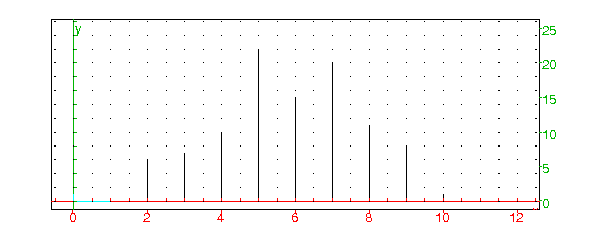
\includegraphics[width=\textwidth]{pain1}

Il suffit de rajouter la ligne dans le programme pr\'ec\'edent 
(au bon enfroit!) :\\
{\tt while (pj<200) \{j:=rand(n); pj:=A[j];\}}\\
qui permet de choisir un pain de poids sup\'erieur ou \'egal \`a 200 grammes.
\begin{verbatim}
chouchou(p,n):={
  local pj,A,P,S,j,k,m;
  P:=makelist(x->0,0,12,1);
  A:=pain(n);
  S:=0;
  for (k:=0;k<p;k++){
    //A:=pain(n);
    j:=rand(n);	
    pj:=A[j];
    //si le poids pj<200g on prend un autre pain
    while (pj<200) {j:=rand(n); pj:=A[j];}
    S:=S+pj;
    pj:=pj-192;
    P[pj]:=P[pj]+1;
  };
  m:=evalf(S/p);
  print(P);
  print(m);
  xyztrange(-0.2,12.2,-1,62.5,-10,10,-10,-10,-0.2,
            12.2,-1,60,1);
  return segment(0,i*P[0]),segment(1,1+i*P[1]),
    segment(2,2+i*P[2]),segment(3,3+i*P[3]),
    segment(4,4+i*P[4]),segment(5,5+i*P[5]),
    segment(6,6+i*P[6]),segment(7,7+i*P[7]),
    segment(8,8+i*P[8]),segment(9,9+i*P[9]),
    segment(10,10+i*P[10]),segment(11,11+i*P[11]),
    segment(12,12+i*P[12]);
};   
\end{verbatim}
On tape : {\tt chouchou(100,1000)} \\ 
On obtient \'ecrit en bleu :\\
{\tt P=[0,0,0,0,0,0,0,0,61,29,6,4,0]}\\
{\tt m=200.53}\\
et le "diagramme en b\^atons" de la distribution des pains 
que le professeur a obtenu  a \'et\'e le suivant :\\

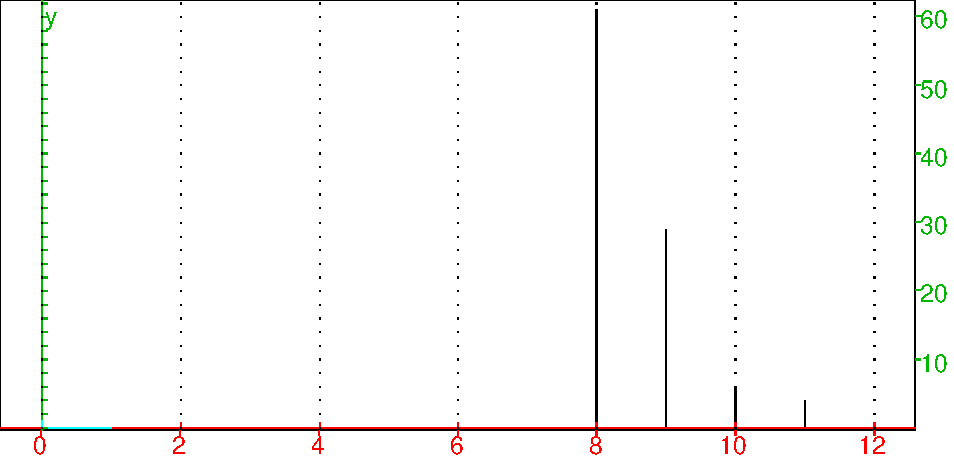
\includegraphics[width=\textwidth]{pain2}
\subsection{Analyse du r\'esultat}
%\section{L}
%\subsection{Simulation}\begin{verbatim}\end{verbatim}\subsection{Analyse du r\'esultat}
\subsection{Simulation avec une loi gaussienne}
On consid\`ere que le poids des pains du boulanger suit une loi gaussienne 
de moyenne 198 grammes et d'\'ecart type $\sigma$ grammes.
\subsubsection{Simulation avec rand()}
Le nombre de pains de poids $x$ est donc approximativement de :\\
$$f(x)=\frac{1}{\sigma \sqrt{2\pi}} e^{-\frac{1}{2}(\frac{x-198}{\sigma})^2}$$ 
Pour  $\sigma=2$ on a :\\
$f(192)=f(204)=0.002 $
$f(193)=f(203)=0.009 $
$f(194)=f(202)=0.027 $
$f(195)=f(201)=0.065 $
$f(196)=f(200)=0.121 $
$f(197)=f(199)=0.176 $
$f(198)=0.200 $

et on a bien $f(192)+f(193)+...+f(204)=1$\\
Voici une fourn\'ee de 1000 pains selon cette r\'epartition repr\'esent\'ee par
la liste {\tt G} des poids de ces 1000 pains.
\begin{verbatim}
//f(x):=0.5/sqrt(2*pi)*exp(-0.125*(x-198)^2)
G:=[192,204,192,204];
for(j:=0;j<9;j++){
G:=concat(G,[193,203]);
};
for(j:=0;j<27;j++){
G:=concat(G,[194,202]);
};
for(j:=0;j<65;j++){
G:=concat(G,[195,201]);
};
for(j:=0;j<121;j++){
G:=concat(G,[196,200]);
};
for(j:=0;j<176;j++){
G:=concat(G,[197,199]);
};
for(j:=0;j<200;j++){
G:=concat(G,[198]);
};
\end{verbatim}
La fourn\'ee {\tt G} de 10000 pains se trouve dans le 
fichier {\tt painG}.\\ 
Le professeur ach\'ete $p$ pains (par exemple $p=100$).
\begin{verbatim}
prof(p):={
local pj,A,P,j,m,S,k;
P:=makelist(0,0,12,1);
A:=G;
S:=0;
for (k:=0;k<p;k++){
    j:=rand(1000);	
    pj:=A[j];
    S:=S+pj;
    pj:=pj-192;
    P[pj]:=P[pj]+1;
};
m:=evalf(S/p);
print(P);
print(m);
return segment(0,i*P[0]),segment(1,1+i*P[1]),
 segment(2,2+i*P[2]),segment(3,3+i*P[3]),
 segment(4,4+i*P[4]),segment(5,5+i*P[5]),
 segment(6,6+i*P[6]),segment(7,7+i*P[7]),
 segment(8,8+i*P[8]),segment(9,9+i*P[9]),
 segment(10,10+i*P[10]),segment(11,11+i*P[11]),
 segment(12,12+i*P[12]);
};  
\end{verbatim}
Le pain du professeur a un poids (en grammes) toujours sup\'erieur ou
\'egal \`a 200.
\begin{verbatim}
profchou(p):={
local pj,A,P,j,m,S,k;
P:=makelist(0,0,12,1);
A:=G;
S:=0;
for (k:=0;k<p;k++){
    j:=rand(1000);	
    pj:=A[j];
    while (pj<200) {j:=rand(n); pj:=A[j];}
    S:=S+pj;
    pj:=pj-192;
    P[pj]:=P[pj]+1;
};
m:=evalf(S/p);
print(P);
print(m);
return segment(0,i*P[0]),segment(1,1+i*P[1]),
 segment(2,2+i*P[2]), segment(3,3+i*P[3]),
 segment(4,4+i*P[4]),segment(5,5+i*P[5]), 
 segment(6,6+i*P[6]),segment(7,7+i*P[7]),
 segment(8,8+i*P[8]), segment(9,9+i*P[9]),
 segment(10,10+i*P[10]),segment(11,11+i*P[11]),
 segment(12,12+i*P[12]);
};  
\end{verbatim}
\subsubsection{Simulation avec {\tt randnorm()}}\index{randnorm}
Pour simuler une fourn\'ee du boulanger, on va utiliser {\tt randnorm(198,2)}
Le professeur ach\'ete $p$ pains (par exemple $p=100$)
\begin{verbatim}
profnorm(p):={
local pj,P,j,m,S,k;
P:=makelist(0,0,12,1);
S:=0;
for (k:=0;k<p;k++){
    pj:=floor(randnorm(198,2));	
    S:=S+pj;
    pj:=pj-192;
    if (pj<0) {P[0]:=P[0]+1;} 
          else
          {if (pj>12) {P[12]:=P[12]+1;}
               else
               {P[pj]:=P[pj]+1;}
           }
};
m:=evalf(S/p);
return([P,m,segment(0,i*P[0]),segment(1,1+i*P[1]),
 segment(2,2+i*P[2]),segment(3,3+i*P[3]),
 segment(4,4+i*P[4]),segment(5,5+i*P[5]),
 segment(6,6+i*P[6]),segment(7,7+i*P[7]),
 segment(8,8+i*P[8]),segment(9,9+i*P[9]),
 segment(10,10+i*P[10]),segment(11,11+i*P[11]),
 segment(12,12+i*P[12])]);
};  
\end{verbatim}
Puis on tape par exemple :\\
{\tt profnorm(100)}
 \'ecrit en bleu :\\
{\tt P=[0,0,0,0,0,0,0,0,61,29,6,4,0]}\\
{\tt m=200.53}\\
et le "diagramme en b\^atons" de la distribution des pains 
On obtient \'ecrit en bleu :\\
{\tt P:[0,2,5,7,13,25,14,16,8,6,3,0,1]}\\
{\tt m:197.66}\\
et le "diagramme en b\^atons" de la distribution des pains selon la loi 
normale de moyenne 198 et d'\'ecart-type 2 :\\

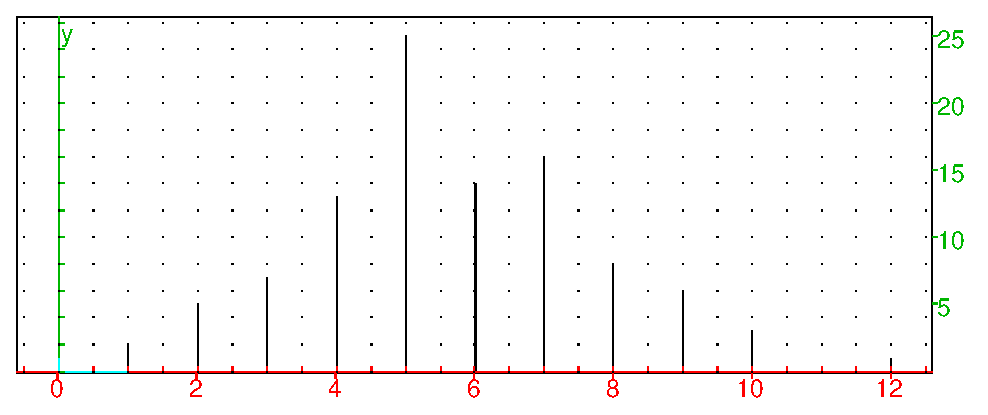
\includegraphics[width=\textwidth]{pain4}

On \'ecrit ensuite le programme {\tt profchounorm} pour simuler
le poids du pain du professeur lorsque ce pain a toujours un poids 
(en grammes) sup\'erieur ou \'egal \`a 200.
\begin{verbatim}
profchounorm(p):={
  local pj,P,j,m,S,k;
  P:=makelist(0,0,12,1);
  S:=0;
  for (k:=0;k<p;k++){
    pj:=floor(randnorm(198,2));	
    while (pj<200) {pj:=floor(randnorm(198,2));}
    S:=S+pj;
    pj:=pj-192;
    if (pj<0) 
     {P[0]:=P[0]+1;} 
    else
     {if (pj>12) {P[12]:=P[12]+1;}
      else
       {P[pj]:=P[pj]+1;}
     };
  };
  m:=evalf(S/p);
  print(P);
  print(m);
  return segment(0,i*P[0]),segment(1,1+i*P[1]),
  segment(2,2+i*P[2]),segment(3,3+i*P[3]),
  segment(4,4+i*P[4]),segment(5,5+i*P[5]),
  segment(6,6+i*P[6]),segment(7,7+i*P[7]),
  segment(8,8+i*P[8]),segment(9,9+i*P[9]),
  segment(10,10+i*P[10]),segment(11,11+i*P[11]),
  segment(12,12+i*P[12]);
};  
\end{verbatim}
On valide ce programme, puis on tape par exemple :\\
{\tt profchounorm(100)}\\
On obtient \'ecrit en bleu :\\
{\tt P=[0,0,0,0,0,0,0,0,60,27,8,4,1]}\\
{\tt m=200.59}\\
et le "diagramme en b\^atons" de la distribution des pains selon la loi normale
de moyenne 198 et d'\'ecart-type 2, pour des poids $p>=200$.\\

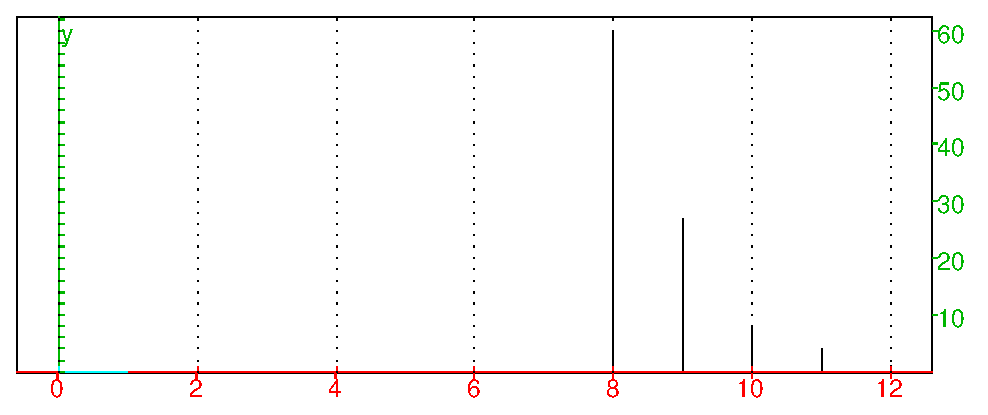
\includegraphics[width=\textwidth]{pain3}

\newpage
\printindex
\newpage
\tableofcontents
\end{document}

%\begin{document}
%\appendix
%Asim
\begin{verbatim}
Asim=[[0.394382926635,0.868641186179],[0.798440032639,0.727895745515],
[0.197551368736,0.466550410103],[0.768229594454,0.213394752973],
[0.553969955072,0.264463623248],[0.628870924003,0.22940234836],
[0.513400909491,0.488875606482],[0.916195067577,0.582435949287],
[0.717296929099,0.101571078062],[0.606968875974,0.00989393934931],
[0.242886770517,0.346786612403],[0.804176753387,0.125997681261],
[0.400944394059,0.478696088765],[0.108808801509,0.999041539081],
[0.218256904744,0.619238261852],[0.839112234302,0.514073578512],
[0.296031617559,0.744848255639],[0.524287189357,0.258779236599],
[0.972775023431,0.284553021226],[0.771357697435,0.406308793753],
[0.769913835451,0.308141552989],[0.891529451124,0.252583439884],
[0.352458346635,0.875493617541],[0.919026473537,0.0641069450682],
[0.949327074923,0.499341626575],[0.0860558478162,0.261728567824],
[0.663226926699,0.590426232761],[0.34889293462,0.390675334961],
[0.0200230488554,0.468560201674],[0.0630958378315,0.28634131812],
[0.970634130761,0.875713948765],[0.850919785909,0.226911162263],
[0.539760340005,0.202521845045],[0.760248735547,0.389654361975],
[0.667723760009,0.354966246897],[0.0392803428695,0.459727384422],
[0.931835055351,0.867361196776],[0.720952342264,0.204961994724],
[0.738534314558,0.47264631606],[0.354048679583,0.798373652382],
[0.165974166244,0.533032711648],[0.880075235851,0.72975934744],
[0.330337129533,0.483668611817],[0.893372413702,0.313002118232],
[0.686669907533,0.656777966478],[0.588640132919,0.386915537018],
[0.85867632553,0.37743969595],[0.923969788477,0.368143442436],
[0.814766895957,0.557478603734],[0.910972029902,0.439535492274],
[0.215824958868,0.960989153102],[0.920128253289,0.135866150964],
[0.881062168628,0.564831859783],[0.431953418069,0.783913082519],
[0.281059412286,0.846148222316],[0.307457873598,0.617047458646],
[0.22610662505,0.371237256036],[0.276234671474,0.678969368316],
[0.41650127992,0.51546679758],[0.906803932972,0.0935560393963],
[0.126075338572,0.559056126113],[0.760475227609,0.748879245897],
[0.935003985651,0.639958817999],[0.383188330568,0.845655759744],
[0.368663541041,0.554377701975],[0.232261538506,0.680995840187],
[0.244412735105,0.359556521084],[0.732148515061,0.091866265127],
[0.793470387347,0.130210024444],[0.745071388781,0.0555300220118],
[0.95010403078,0.04990826392],[0.521563379094,0.0919050250875],
[0.240062371828,0.846339130844],[0.732654411346,0.481034256465],
[0.967405137606,0.618615288479],[0.759734841064,0.0710203754194],
[0.134902411141,0.584934888056],[0.0782321412116,0.142669611756],
[0.20465508569,0.57164351202],[0.819677279331,0.469936252912],
[0.755580835044,0.0392439760557],[0.157807128504,0.999994584825],
[0.204328610562,0.912440854015],[0.125468475744,0.998075155101],
[0.0540575776249,0.877538165848],[0.0723287994042,0.0761894036701],
[0.923069126904,0.548203534681],[0.180372265168,0.314079365953],
[0.391690229997,0.947093277593],[0.819695152342,0.294348732816],
[0.552485021763,0.320126392517],[0.452575845644,0.828868330326],
[0.0996400630102,0.577558309448],[0.757293831557,0.230440839789],
[0.992228460498,0.572487158032],[0.877613777295,0.656287740557],
[0.628909930587,0.0222765599929],[0.747802866623,0.623098169652],
[0.925376550294,0.808104822271],[0.831037539989,0.813946529021]]
moyenne=0.35
\end{verbatim}
%Aex
\begin{verbatim}
Aex:=
[[0.772150173038,0.32083329334],[0.726479378343,0.536688112678],
[0.829317885637,0.213998095303],[0.368178204447,0.819667745414],
[0.322219768167,0.690373699012],[0.481917641312,0.794371422475],
[0.391827578098,0.702433839913],[0.861783779413,0.717828016354],
[0.608569382131,0.41007689737],[0.213282044232,0.673964490466],
[0.113040456921,0.374081002427],[0.209785261005,0.797184593531],
[0.225343271345,0.55128436235],[0.203832357377,0.352753159235],
[0.899139613658,0.246908704573],[0.51034591496,0.393624592271],
[0.590111865848,0.198764602735],[0.610041813552,0.316873867609],
[0.494866389036,0.938484838325],[0.334013427049,0.811583179891],
[0.521395982802,0.373283583006],[0.420182897151,0.8917038262],
[0.326651796699,0.583848372585],[0.746179615706,0.623225018249],
[0.155804220587,0.881358126474],[0.520796279609,0.0879336802659],
[0.253771076351,0.724329261233],[0.812186081707,0.307911396575],
[0.151337056607,0.249797606608],[0.466161389649,0.546491646194],
[0.290623962879,0.91239724113],[0.821766458452,0.64158251696],
[0.313332599401,0.678508003155],[0.400165580958,0.824967709754],
[0.510028290749,0.323449235482],[0.52528514713,0.0690352192599],
[0.450110077113,0.915024434786],[0.84464783594,0.571625452162],
[0.327434722334,0.79206127917],[0.611983052641,0.234535738636],
[0.650289111584,0.151373865649],[0.452083621919,0.89264136826],
[0.763360874355,0.278069239461],[0.283174536377,0.867170758451],
[0.380288142711,0.782689315433],[0.865174601972,0.49393865436],
[0.62584323138,0.492501736161],[0.451647935063,0.911811734717],
[0.418749333173,0.855741441123],[0.647374819964,0.536529765077],
[0.485992524773,0.626141786055],[0.860201898962,0.71921704651],
[0.218128011376,0.847417474148],[0.612864476442,0.273069571974],
[0.595677186549,0.193504262626],[0.728801678121,0.252140819196],
[0.457626862824,0.609971504193],[0.250026487559,0.490758788262],
[0.545155003667,0.236161705792],[0.235685668886,0.866583695182],
[0.182536950707,0.346732800205],[0.496355252713,0.853127210504],
[0.887801331282,0.7528583597],[0.647556012869,0.263264327303],
[0.699816705287,0.276379194249],[0.335328289121,0.525297599545],
[0.567590799928,0.167740215857],[0.221911833435,0.755461526681],
[0.200379923731,0.787921812676],[0.231281546503,0.766353492436],
[0.159623840451,0.882417277653],[0.142023409903,0.585812404524],
[0.240968524665,0.462643589207],[0.738238441199,0.506522764575],
[0.625250922143,0.546421855714],[0.611566676199,0.432859476854],
[0.174784381688,0.346364804816],[0.516168055683,0.0839215513453],
[0.155925118178,0.378527980175],[0.469136378169,0.870332219743],
[0.55865490213,0.393552640176],[0.141551055014,0.335771439893],
[0.899994856119,0.237115244383],[0.811964514852,0.162697211515],
[0.898239199072,0.128669228091],[0.79643189162,0.125727159185],
[0.103329286724,0.855147599991],[0.575113742799,0.140499029094],
[0.230505198985,0.54857755556],[0.830421341211,0.627596012355],
[0.387276294827,0.719365201014],[0.563543994725,0.260391519449],
[0.649909947067,0.116796649168],[0.524646390229,0.370313819078],
[0.343436119705,0.930261602266],[0.561576889455,0.450435781103],
[0.698247436434,0.421132541068],[0.128336725384,0.736968889236],
[0.766590832919,0.644167227655],[0.798617073894,0.610806322175]]
moyenne=0.5
\end{verbatim}

%painA
A:= [195,199,198,196,201,197,198,199,198,199,197,199,198,201,
197,199,201,200,195,199,197,200,196,200,199,197,197,197,196,199,
202,198,197,201,202,200,198,199,196,200,196,198,199,198,198,198,
199,197,199,199,198,196,197,197,198,198,197,197,200,197,200,196,
198,194,197,197,197,198,196,198,200,196,195,193,196,197,197,196,
196,200,198,198,199,198,198,196,198,199,198,198,198,200,196,198,
196,202,195,198,199,197,199,198,198,199,194,195,197,200,198,198,
199,197,196,198,200,202,197,198,198,198,193,200,198,198,196,199,
196,201,200,197,199,200,195,197,201,198,198,199,199,197,197,198,
197,194,198,199,198,198,196,197,199,196,195,197,198,197,198,195,
199,199,197,197,197,198,197,199,195,200,196,195,198,198,199,196,
197,199,200,196,197,194,198,195,197,199,199,202,195,196,197,195,
197,197,196,197,199,201,198,201,196,199,200,199,198,198,194,199,
199,199,196,198,201,199,197,197,197,197,197,196,199,199,200,198,
199,201,198,197,197,195,199,198,197,200,197,199,197,199,196,197,
197,197,197,195,198,197,199,198,200,198,200,196,197,195,198,195,
198,197,198,198,200,197,202,196,195,196,197,196,200,198,199,196,
196,195,198,197,198,198,199,197,199,198,197,198,197,196,197,199,
198,198,199,201,200,196,196,198,199,199,195,197,200,198,198,198,
198,198,199,198,198,202,200,198,198,197,196,199,196,193,200,198,
199,201,198,197,199,196,203,201,197,198,198,199,200,199,200,197,
196,196,196,197,200,196,196,199,198,198,196,199,196,199,201,199,
198,200,195,197,198,198,199,199,198,200,199,199,196,198,196,198,
196,199,202,196,196,196,199,197,198,198,198,195,199,195,200,202,
198,198,196,199,198,199,194,197,198,196,198,200,194,200,198,194,
203,200,197,195,199,201,198,198,198,199,196,197,196,198,197,200,
199,198,195,195,198,201,198,196,195,198,197,197,198,200,199,196,
198,201,198,197,196,200,199,197,200,197,198,198,199,196,201,198,
197,197,199,196,200,198,197,200,199,196,198,196,197,198,200,197,
196,197,193,200,198,201,194,198,196,195,198,196,197,192,198,196,
197,197,198,197,198,199,196,194,199,199,198,200,200,199,200,197,
198,200,197,199,197,199,199,196,196,198,200,201,199,201,196,200,
195,198,198,199,198,198,200,197,197,197,199,199,197,198,199,198,
197,197,198,202,197,199,199,199,199,199,197,200,200,198,197,195,
194,196,198,198,199,201,198,198,199,196,200,198,198,197,199,198,
202,196,198,198,199,198,202,198,198,202,198,197,198,199,201,197,
197,201,200,199,199,199,196,198,199,199,198,199,196,198,197,197,
197,201,197,197,196,197,198,198,199,196,199,198,196,196,201,197,
196,198,196,198,194,199,199,199,197,196,195,200,198,198,196,199,
200,199,199,203,198,198,201,197,200,199,198,199,196,200,199,195,
200,200,198,199,196,200,196,197,197,200,198,197,197,198,198,200,
200,199,197,198,196,197,199,195,195,197,196,201,200,198,197,200,
198,199,199,196,199,198,199,195,198,197,198,197,200,198,198,196,
202,198,199,200,199,199,197,196,201,197,198,198,202,195,199,200,
201,200,199,198,197,195,200,199,198,198,197,200,201,198,199,199,
198,196,196,202,196,199,199,201,201,198,199,201,199,199,198,200,
198,196,201,198,199,199,199,198,197,197,196,196,201,198,198,197,
199,198,198,197,194,195,198,199,199,197,198,197,199,200,197,199,
197,200,198,198,195,202,201,199,195,196,200,197,194,199,196,196,
197,196,200,201,200,197,199,198,198,198,199,201,199,195,195,199,
199,200,197,199,198,196,194,198,198,200,200,195,196,199,198,198,
198,197,198,199,199,198,198,195,200,199,198,197,198,199,201,197,
199,196,197,200,197,197,198,198,193,196,196,197,194,199,198,198,
199,198,199,198,197,199,196,196,197,198,200,199,201,199,203,199,
199,199,199,202,197,196,198,198,197,197,198,197,198,199,197,198,
198,198,194,197,200,198,199,200,200,197,197,200,199,197,201,200,
198,196,196,197,201,198,198,199,200,200,198,201,198,195,197,199,
199,197,192,198,197,197,195,199,195,199,199,197,198,199,200,201,
199,197,199,197,198,195,198,199,197,194,201,200,197,196,197,198,
194,195,197,200,196,198,197,197,198,198,198,198,195,199,196,200,
196,197,200,193,199,198,197,196,197,200,196,196,197,200,199,198,
198,202,198,195,199,195,198,196,199,198,197,199,200,198,196,200,
198,199,197,199,199,196,199,201,200,197]
%painG

G:=[192,204,192,204,
193,203,193,203,193,203,193,203,193,203,193,203,193,203,193,203,193,203,
194,202,194,202,194,202,194,202,194,202,194,202,194,202,194,202,194,202,
194,202,194,202,194,202,194,202,194,202,194,202,194,202,194,202,194,202,
194,202,194,202,194,202,194,202,194,202,194,202,194,202,194,202,194,202,
195,201,195,201,195,201,195,201,195,201,195,201,195,201,195,201,195,201,
195,201,195,201,195,201,195,201,195,201,195,201,195,201,195,201,195,201,
195,201,195,201,195,201,195,201,195,201,195,201,195,201,195,201,195,201,
195,201,195,201,195,201,195,201,195,201,195,201,195,201,195,201,195,201,
195,201,195,201,195,201,195,201,195,201,195,201,195,201,195,201,195,201,
195,201,195,201,195,201,195,201,195,201,195,201,195,201,195,201,195,201,
195,201,195,201,195,201,195,201,195,201,195,201,195,201,195,201,195,201,
195,201,195,201,
196,200,196,200,196,200,196,200,196,200,196,200,196,200,196,200,196,200,
196,200,196,200,196,200,196,200,196,200,196,200,196,200,196,200,196,200,
196,200,196,200,196,200,196,200,196,200,196,200,196,200,196,200,196,200,
196,200,196,200,196,200,196,200,196,200,196,200,196,200,196,200,196,200,
196,200,196,200,196,200,196,200,196,200,196,200,196,200,196,200,196,200,
196,200,196,200,196,200,196,200,196,200,196,200,196,200,196,200,196,200,
196,200,196,200,196,200,196,200,196,200,196,200,196,200,196,200,196,200,
196,200,196,200,196,200,196,200,196,200,196,200,196,200,196,200,196,200,
196,200,196,200,196,200,196,200,196,200,196,200,196,200,196,200,196,200,
196,200,196,200,196,200,196,200,196,200,196,200,196,200,196,200,196,200,
196,200,196,200,196,200,196,200,196,200,196,200,196,200,196,200,196,200,
196,200,196,200,196,200,196,200,196,200,196,200,196,200,196,200,196,200,
196,200,196,200,196,200,196,200,196,200,196,200,196,200,196,200,196,200,
196,200,196,200,196,200,196,200,
197,199,197,199,197,199,197,199,197,199,197,199,197,199,197,199,197,199,
197,199,197,199,197,199,197,199,197,199,197,199,197,199,197,199,197,199,
197,199,197,199,197,199,197,199,197,199,197,199,197,199,197,199,197,199,
197,199,197,199,197,199,197,199,197,199,197,199,197,199,197,199,197,199,
197,199,197,199,197,199,197,199,197,199,197,199,197,199,197,199,197,199,
197,199,197,199,197,199,197,199,197,199,197,199,197,199,197,199,197,199,
197,199,197,199,197,199,197,199,197,199,197,199,197,199,197,199,197,199,
197,199,197,199,197,199,197,199,197,199,197,199,197,199,197,199,197,199,
197,199,197,199,197,199,197,199,197,199,197,199,197,199,197,199,197,199,
197,199,197,199,197,199,197,199,197,199,197,199,197,199,197,199,197,199,
197,199,197,199,197,199,197,199,197,199,197,199,197,199,197,199,197,199,
197,199,197,199,197,199,197,199,197,199,197,199,197,199,197,199,197,199,
197,199,197,199,197,199,197,199,197,199,197,199,197,199,197,199,197,199,
197,199,197,199,197,199,197,199,197,199,197,199,197,199,197,199,197,199,
197,199,197,199,197,199,197,199,197,199,197,199,197,199,197,199,197,199,
197,199,197,199,197,199,197,199,197,199,197,199,197,199,197,199,197,199,
197,199,197,199,197,199,197,199,197,199,197,199,197,199,197,199,197,199,
197,199,197,199,197,199,197,199,197,199,197,199,197,199,197,199,197,199,
197,199,197,199,197,199,197,199,197,199,197,199,197,199,197,199,197,199,
197,199,197,199,197,199,197,199,197,199,
198,198,198,198,198,198,198,198,198,198,198,198,198,198,198,198,198,198,
198,198,198,198,198,198,198,198,198,198,198,198,198,198,198,198,198,198,
198,198,198,198,198,198,198,198,198,198,198,198,198,198,198,198,198,198,
198,198,198,198,198,198,198,198,198,198,198,198,198,198,198,198,198,198,
198,198,198,198,198,198,198,198,198,198,198,198,198,198,198,198,198,198,
198,198,198,198,198,198,198,198,198,198,198,198,198,198,198,198,198,198,
198,198,198,198,198,198,198,198,198,198,198,198,198,198,198,198,198,198,
198,198,198,198,198,198,198,198,198,198,198,198,198,198,198,198,198,198,
198,198,198,198,198,198,198,198,198,198,198,198,198,198,198,198,198,198,
198,198,198,198,198,198,198,198,198,198,198,198,198,198,198,198,198,198,
198,198,198,198,198,198,198,198,198,198,198,198,198,198,198,198,198,198,
198,198]

%figure 1
\noindent
\begin{pspicture}(0.0000,-2.0000)(8.0000,3.0000)
\psset{linewidth=.5pt}
\psset{arrowsize=2pt 4}
\psset{linecolor=black}
\psline[linestyle=dashed]{->}(0.0000,0.0000)(8.0000,0.0000)
\psline[linestyle=dashed]{->}(0.0000,-2.0000)(0.0000,3.0000)
\psset{linecolor=black}
\psset{linecolor=black}
\psline(0.0000,1.3416)(2.0000,1.3416)
\psset{linecolor=black}
\psline(2.0000,1.1770)(2.0000,1.5062)
\psset{linecolor=black}
\psline(4.0000,1.1770)(4.0000,1.5062)
\psset{linecolor=black}
\psline(6.0000,1.1770)(6.0000,1.5062)
\psset{linecolor=black}
\psline(2.0000,1.5062)(6.0000,1.5062)
\psset{linecolor=black}
\psline(2.0000,1.1770)(6.0000,1.1770)
\psset{linecolor=black}
\psline(6.0000,1.3416)(8.0000,1.3416)
\psset{linecolor=black}
\psline(1.0,0)(1.0,0.05)
\psline(2.0,0)(2.0,0.05)
\psline(3.0,0)(3.0,0.05)
\psline(4.0,0)(4.0,0.05)
\psline(5.0,0)(5.0,0.05)
\psline(6.0,0)(6.0,0.05)
\psline(7.0,0)(7.0,0.05)
\end{pspicture}


% figure 2
\noindent
\begin{pspicture}(0,0)(5.2000,8.0000)
\psset{unit=0.5cm}
\psset{linewidth=.5pt}
\psset{arrowsize=2pt 4}
\psset{linecolor=black}
\psset{linecolor=green}
\psdots[dotstyle=*](0.0000,0.4045)
\psset{linecolor=black}
\psline(0.0000,0.0000)(0.0000,0.0000)
\psset{linecolor=black}
\psline(1.0000,0.0000)(1.0000,4.0000)
\psset{linecolor=black}
\psline(2.0000,0.0000)(2.0000,14.0000)
\psset{linecolor=black}
\psline(3.0000,0.0000)(3.0000,6.0000)
\psset{linecolor=black}
\psline(4.0000,0.0000)(4.0000,6.0000)
\psset{linecolor=black}
\psline(5.0000,0.0000)(5.0000,0.0000)
\end{pspicture}

% figure 3
\noindent
\begin{pspicture}(0,0)(12.2000,12.0000)
\psset{unit=0.3871cm}
\psset{linewidth=.5pt}
\psset{arrowsize=2pt 4}
\psset{linecolor=black}
\psset{linecolor=green}
\psdots[dotstyle=*](8.0000,20.8121)
\psset{linecolor=green}
\psdots[dotstyle=*](8.0000,0.7121)
\psset{linecolor=black}
\psline(0.0000,0.0000)(0.0000,1.0000)
\psset{linecolor=black}
\psline(1.0000,0.0000)(1.0000,1.0000)
\psset{linecolor=black}
\psline(2.0000,0.0000)(2.0000,1.0000)
\psset{linecolor=black}
\psline(3.0000,0.0000)(3.0000,3.0000)
\psset{linecolor=black}
\psline(4.0000,0.0000)(4.0000,14.0000)
\psset{linecolor=black}
\psline(5.0000,0.0000)(5.0000,16.0000)
\psset{linecolor=black}
\psline(6.0000,0.0000)(6.0000,34.0000)
\psset{linecolor=black}
\psline(7.0000,0.0000)(7.0000,17.0000)
\psset{linecolor=black}
\psline(8.0000,0.0000)(8.0000,5.0000)
\psset{linecolor=black}
\psline(9.0000,0.0000)(9.0000,5.0000)
\psset{linecolor=black}
\psline(10.0000,0.0000)(10.0000,3.0000)
\psset{linecolor=black}
\psline(11.0000,0.0000)(11.0000,0.0000)
\psset{linecolor=black}
\psline(12.0000,0.0000)(12.0000,0.0000)
\end{pspicture}

% figure 4
\noindent
\begin{pspicture}(0,0)(12.2000,12.0000)
\psset{unit=0.1967cm}
\psset{linewidth=.5pt}
\psset{arrowsize=2pt 4}
\psset{linecolor=black}
\psset{linecolor=black}
\psline(0.0000,0.0000)(0.0000,0.0000)
\psset{linecolor=black}
\psline(1.0000,0.0000)(1.0000,0.0000)
\psset{linecolor=black}
\psline(2.0000,0.0000)(2.0000,0.0000)
\psset{linecolor=black}
\psline(3.0000,0.0000)(3.0000,0.0000)
\psset{linecolor=black}
\psline(4.0000,0.0000)(4.0000,0.0000)
\psset{linecolor=black}
\psline(5.0000,0.0000)(5.0000,0.0000)
\psset{linecolor=black}
\psline(6.0000,0.0000)(6.0000,0.0000)
\psset{linecolor=black}
\psline(7.0000,0.0000)(7.0000,0.0000)
\psset{linecolor=black}
\psline(8.0000,0.0000)(8.0000,69.0000)
\psset{linecolor=black}
\psline(9.0000,0.0000)(9.0000,24.0000)
\psset{linecolor=black}
\psline(10.0000,0.0000)(10.0000,7.0000)
\psset{linecolor=black}
\psline(11.0000,0.0000)(11.0000,0.0000)
\psset{linecolor=black}
\psline(12.0000,0.0000)(12.0000,0.0000)
\end{pspicture}

%file figure5
% Generated by Xcas
\noindent
\begin{pspicture}(0,0)(12.2000,12.0000)
\psset{unit=0.1967cm}
\psset{linewidth=.5pt}
\psset{arrowsize=2pt 4}
\psset{linecolor=black}
\psset{linecolor=black}
\psline(0.0000,0.0000)(0.0000,0.0000)
\psset{linecolor=black}
\psline(1.0000,0.0000)(1.0000,0.0000)
\psset{linecolor=black}
\psline(2.0000,0.0000)(2.0000,0.0000)
\psset{linecolor=black}
\psline(3.0000,0.0000)(3.0000,0.0000)
\psset{linecolor=black}
\psline(4.0000,0.0000)(4.0000,0.0000)
\psset{linecolor=black}
\psline(5.0000,0.0000)(5.0000,0.0000)
\psset{linecolor=black}
\psline(6.0000,0.0000)(6.0000,0.0000)
\psset{linecolor=black}
\psline(7.0000,0.0000)(7.0000,0.0000)
\psset{linecolor=black}
\psline(8.0000,0.0000)(8.0000,60.0000)
\psset{linecolor=black}
\psline(9.0000,0.0000)(9.0000,21.0000)
\psset{linecolor=black}
\psline(10.0000,0.0000)(10.0000,12.0000)
\psset{linecolor=black}
\psline(11.0000,0.0000)(11.0000,5.0000)
\psset{linecolor=black}
\psline(12.0000,0.0000)(12.0000,2.0000)
\end{pspicture}

%uni.cas
spreadsheet[[[rand(0 .. 1),0.864446785301,2],[rand(0 .. 1),0.235939053819,2],[rand(0 .. 1),0.589939414524,2],[rand(0 .. 1),0.384632935282,2],[rand(0 .. 1),0.66865148209,2],[=mean((A0):(E0)),0.548721934203,2],[=stddev((A0):(E0)),0.21932737566,2]],[[rand(0 .. 1),0.0837768828496,2],[rand(0 .. 1),0.923186001834,2],[rand(0 .. 1),0.536572443321,2],[rand(0 .. 1),0.0241006566212,2],[rand(0 .. 1),0.167277826928,2],[=mean((A1):(E1)),0.346982762311,2],[=stddev((A1):(E1)),0.338756099086,2]],[[rand(0 .. 1),0.741091293283,2],[rand(0 .. 1),0.332505674567,2],[rand(0 .. 1),0.976268766914,2],[rand(0 .. 1),0.155812136829,2],[rand(0 .. 1),0.614800942596,2],[=mean((A2):(E2)),0.564095762838,2],[=stddev((A2):(E2)),0.291243714642,2]],[[rand(0 .. 1),0.611356332898,2],[rand(0 .. 1),0.748605543748,2],[rand(0 .. 1),0.139356779866,2],[rand(0 .. 1),0.852039497346,2],[rand(0 .. 1),0.978510552086,2],[=mean((A3):(E3)),0.665973741189,2],[=stddev((A3):(E3)),0.289632948338,2]],[[rand(0 .. 1),0.780953796115,2],[rand(0 .. 1),0.853436828591,2],[rand(0 .. 1),0.246799692977,2],[rand(0 .. 1),0.339623136912,2],[rand(0 .. 1),0.982576256618,2],[=mean((A4):(E4)),0.640677942242,2],[=stddev((A4):(E4)),0.292442195085,2]],[[rand(0 .. 1),0.688296142966,2],[rand(0 .. 1),0.948739923537,2],[rand(0 .. 1),0.0375739675947,2],[rand(0 .. 1),0.673975562677,2],[rand(0 .. 1),0.445936217438,2],[=mean((A5):(E5)),0.558904362842,2],[=stddev((A5):(E5)),0.305451325439,2]],[[rand(0 .. 1),0.504968397319,2],[rand(0 .. 1),0.538422347978,2],[rand(0 .. 1),0.681875271257,2],[rand(0 .. 1),0.0949078118429,2],[rand(0 .. 1),0.92305528326,2],[=mean((A6):(E6)),0.548645822331,2],[=stddev((A6):(E6)),0.27048953752,2]],[[rand(0 .. 1),0.350526753347,2],[rand(0 .. 1),0.178684694692,2],[rand(0 .. 1),0.846241285559,2],[rand(0 .. 1),0.887099197134,2],[rand(0 .. 1),0.202785351314,2],[=mean((A7):(E7)),0.493067456409,2],[=stddev((A7):(E7)),0.310937562777,2]],[[rand(0 .. 1),0.0135191124864,2],[rand(0 .. 1),0.628190490417,2],[rand(0 .. 1),0.535291025881,2],[rand(0 .. 1),0.9897878794,2],[rand(0 .. 1),0.784002627246,2],[=mean((A8):(E8)),0.590158227086,2],[=stddev((A8):(E8)),0.326878889435,2]],[[rand(0 .. 1),0.150091968942,2],[rand(0 .. 1),0.601144212298,2],[rand(0 .. 1),0.532608170994,2],[rand(0 .. 1),0.289448748808,2],[rand(0 .. 1),0.453183709644,2],[=mean((A9):(E9)),0.405295362137,2],[=stddev((A9):(E9)),0.164564775668,2]],[[rand(0 .. 1),0.51111872308,2],[rand(0 .. 1),0.0704025449231,2],[rand(0 .. 1),0.306620538235,2],[rand(0 .. 1),0.757918416057,2],[rand(0 .. 1),0.410025681835,2],[=mean((A10):(E10)),0.411217180826,2],[=stddev((A10):(E10)),0.226838514372,2]],[[rand(0 .. 1),0.289196795318,2],[rand(0 .. 1),0.446214559022,2],[rand(0 .. 1),0.358765605837,2],[rand(0 .. 1),0.326770762913,2],[rand(0 .. 1),0.120190121699,2],[=mean((A11):(E11)),0.308227568958,2],[=stddev((A11):(E11)),0.107385850611,2]],[[rand(0 .. 1),0.804701823276,2],[rand(0 .. 1),0.831739160232,2],[rand(0 .. 1),0.658612469677,2],[rand(0 .. 1),0.486577094533,2],[rand(0 .. 1),0.926646972075,2],[=mean((A12):(E12)),0.741655503958,2],[=stddev((A12):(E12)),0.153800446866,2]],[[rand(0 .. 1),0.581667753402,2],[rand(0 .. 1),0.83710384788,2],[rand(0 .. 1),0.105331666768,2],[rand(0 .. 1),0.427909038961,2],[rand(0 .. 1),0.724203045014,2],[=mean((A13):(E13)),0.535243070405,2],[=stddev((A13):(E13)),0.255078600222,2]],[[rand(0 .. 1),0.308117018547,2],[rand(0 .. 1),0.441428151447,2],[rand(0 .. 1),0.352393535431,2],[rand(0 .. 1),0.843408044428,2],[rand(0 .. 1),0.431216030847,2],[=mean((A14):(E14)),0.47531255614,2],[=stddev((A14):(E14)),0.190604500663,2]],[[rand(0 .. 1),0.136396162678,2],[rand(0 .. 1),0.99350001337,2],[rand(0 .. 1),0.0323602431454,2],[rand(0 .. 1),0.669004333671,2],[rand(0 .. 1),0.282948762178,2],[=mean((A15):(E15)),0.422841903009,2],[=stddev((A15):(E15)),0.357866958767,2]],[[rand(0 .. 1),0.485543952789,2],[rand(0 .. 1),0.180123057216,2],[rand(0 .. 1),0.353351307567,2],[rand(0 .. 1),0.79216449149,2],[rand(0 .. 1),0.938041473273,2],[=mean((A16):(E16)),0.549844856467,2],[=stddev((A16):(E16)),0.278874146751,2]],[[rand(0 .. 1),0.763376989402,2],[rand(0 .. 1),0.0813612868078,2],[rand(0 .. 1),0.384256032761,2],[rand(0 .. 1),0.122142595239,2],[rand(0 .. 1),0.408132049721,2],[=mean((A17):(E17)),0.351853790786,2],[=stddev((A17):(E17)),0.244745549002,2]],[[rand(0 .. 1),0.50444615446,2],[rand(0 .. 1),0.926844418515,2],[rand(0 .. 1),0.239871210419,2],[rand(0 .. 1),0.163058624603,2],[rand(0 .. 1),0.413421513047,2],[=mean((A18):(E18)),0.449528384209,2],[=stddev((A18):(E18)),0.267645780064,2]],[[rand(0 .. 1),0.166518182494,2],[rand(0 .. 1),0.744726378005,2],[rand(0 .. 1),0.250525361393,2],[rand(0 .. 1),0.271849849727,2],[rand(0 .. 1),0.172635416966,2],[=mean((A19):(E19)),0.321251037717,2],[=stddev((A19):(E19)),0.21577897104,2]],[[rand(0 .. 1),0.974728406407,2],[rand(0 .. 1),0.579966868274,2],[rand(0 .. 1),0.614063568413,2],[rand(0 .. 1),0.327121942304,2],[rand(0 .. 1),0.423374912702,2],[=mean((A20):(E20)),0.58385113962,2],[=stddev((A20):(E20)),0.221528967076,2]],[[rand(0 .. 1),0.0452795992605,2],[rand(0 .. 1),0.463518104982,2],[rand(0 .. 1),0.416874926537,2],[rand(0 .. 1),0.0776398424059,2],[rand(0 .. 1),0.132522439118,2],[=mean((A21):(E21)),0.227166982461,2],[=stddev((A21):(E21)),0.176776657128,2]],[[rand(0 .. 1),0.699823688716,2],[rand(0 .. 1),0.563183795195,2],[rand(0 .. 1),0.312645496335,2],[rand(0 .. 1),0.0531749962829,2],[rand(0 .. 1),0.355348286685,2],[=mean((A22):(E22)),0.396835252643,2],[=stddev((A22):(E22)),0.221984362159,2]],[[rand(0 .. 1),0.250686969608,2],[rand(0 .. 1),0.81655198615,2],[rand(0 .. 1),0.436709573492,2],[rand(0 .. 1),0.634943002369,2],[rand(0 .. 1),0.938694581389,2],[=mean((A23):(E23)),0.615517222602,2],[=stddev((A23):(E23)),0.249122151238,2]],[[rand(0 .. 1),0.844841623679,2],[rand(0 .. 1),0.139389157295,2],[rand(0 .. 1),0.86553900037,2],[rand(0 .. 1),0.0847128340974,2],[rand(0 .. 1),0.302447781898,2],[=mean((A24):(E24)),0.447386079468,2],[=stddev((A24):(E24)),0.340653452048,2]],[[rand(0 .. 1),0.278960513417,2],[rand(0 .. 1),0.251231016591,2],[rand(0 .. 1),0.0471741599031,2],[rand(0 .. 1),0.529485874809,2],[rand(0 .. 1),0.523080866318,2],[=mean((A25):(E25)),0.325986486208,2],[=stddev((A25):(E25)),0.182095761338,2]],[[rand(0 .. 1),0.219809576869,2],[rand(0 .. 1),0.504214281682,2],[rand(0 .. 1),0.103047734592,2],[rand(0 .. 1),0.833873145282,2],[rand(0 .. 1),0.831336223986,2],[=mean((A26):(E26)),0.498456192482,2],[=stddev((A26):(E26)),0.302436303428,2]],[[rand(0 .. 1),0.526422647759,2],[rand(0 .. 1),0.879152744543,2],[rand(0 .. 1),0.294854328968,2],[rand(0 .. 1),0.943297574297,2],[rand(0 .. 1),0.956792586949,2],[=mean((A27):(E27)),0.720103976503,2],[=stddev((A27):(E27)),0.264379693191,2]],[[rand(0 .. 1),0.427376768086,2],[rand(0 .. 1),0.643121263012,2],[rand(0 .. 1),0.519976382144,2],[rand(0 .. 1),0.740022264421,2],[rand(0 .. 1),0.696296259761,2],[=mean((A28):(E28)),0.605358587485,2],[=stddev((A28):(E28)),0.11558341993,2]],[[rand(0 .. 1),0.875324669294,2],[rand(0 .. 1),0.990709234495,2],[rand(0 .. 1),0.512848245911,2],[rand(0 .. 1),0.312034242786,2],[rand(0 .. 1),0.625652236864,2],[=mean((A29):(E29)),0.66331372587,2],[=stddev((A29):(E29)),0.244782345298,2]],[[rand(0 .. 1),0.451542827301,2],[rand(0 .. 1),0.156875866465,2],[rand(0 .. 1),0.765041394159,2],[rand(0 .. 1),0.31708182767,2],[rand(0 .. 1),0.241588700563,2],[=mean((A30):(E30)),0.386426123232,2],[=stddev((A30):(E30)),0.212635622247,2]],[[rand(0 .. 1),0.0674891760573,2],[rand(0 .. 1),0.596042341553,2],[rand(0 .. 1),0.49281971762,2],[rand(0 .. 1),0.11466333596,2],[rand(0 .. 1),0.125528216362,2],[=mean((A31):(E31)),0.27930855751,2],[=stddev((A31):(E31)),0.21978680493,2]],[[rand(0 .. 1),0.0159005839378,2],[rand(0 .. 1),0.334472912829,2],[rand(0 .. 1),0.629742498044,2],[rand(0 .. 1),0.118948318996,2],[rand(0 .. 1),0.168346058112,2],[=mean((A32):(E32)),0.253482074384,2],[=stddev((A32):(E32)),0.214440602281,2]],[[rand(0 .. 1),0.46107872203,2],[rand(0 .. 1),0.645370966755,2],[rand(0 .. 1),0.0474988026544,2],[rand(0 .. 1),0.755933051463,2],[rand(0 .. 1),0.588668541051,2],[=mean((A33):(E33)),0.499710016791,2],[=stddev((A33):(E33)),0.245262444743,2]],[[rand(0 .. 1),0.00429138960317,2],[rand(0 .. 1),0.183309819549,2],[rand(0 .. 1),0.231789804064,2],[rand(0 .. 1),0.524267772213,2],[rand(0 .. 1),0.923332084436,2],[=mean((A34):(E34)),0.373398173973,2],[=stddev((A34):(E34)),0.321749987641,2]],[[rand(0 .. 1),0.928086063825,2],[rand(0 .. 1),0.399592441507,2],[rand(0 .. 1),0.914041318931,2],[rand(0 .. 1),0.440934309736,2],[rand(0 .. 1),0.711626684293,2],[=mean((A35):(E35)),0.678856163658,2],[=stddev((A35):(E35)),0.224987351868,2]],[[rand(0 .. 1),0.539693555795,2],[rand(0 .. 1),0.892477137502,2],[rand(0 .. 1),0.868502551224,2],[rand(0 .. 1),0.30473495042,2],[rand(0 .. 1),0.209558965173,2],[=mean((A36):(E36)),0.562993432023,2],[=stddev((A36):(E36)),0.280731752391,2]],[[rand(0 .. 1),0.110091251787,2],[rand(0 .. 1),0.372224126477,2],[rand(0 .. 1),0.805601306725,2],[rand(0 .. 1),0.602910969406,2],[rand(0 .. 1),0.486887462903,2],[=mean((A37):(E37)),0.47554302346,2],[=stddev((A37):(E37)),0.232172156903,2]],[[rand(0 .. 1),0.931129523553,2],[rand(0 .. 1),0.61881155381,2],[rand(0 .. 1),0.821360375732,2],[rand(0 .. 1),0.560872021597,2],[rand(0 .. 1),0.737759872805,2],[=mean((A38):(E38)),0.733986669499,2],[=stddev((A38):(E38)),0.133975889697,2]],[[rand(0 .. 1),0.989706434309,2],[rand(0 .. 1),0.0219507440925,2],[rand(0 .. 1),0.38313083956,2],[rand(0 .. 1),0.0372052369639,2],[rand(0 .. 1),0.777883795556,2],[=mean((A39):(E39)),0.441975410096,2],[=stddev((A39):(E39)),0.388989977994,2]],[[rand(0 .. 1),0.971799380612,2],[rand(0 .. 1),0.0414966270328,2],[rand(0 .. 1),0.961193615105,2],[rand(0 .. 1),0.203589184675,2],[rand(0 .. 1),0.565764399245,2],[=mean((A40):(E40)),0.548768641334,2],[=stddev((A40):(E40)),0.381001830689,2]],[[rand(0 .. 1),0.884525699541,2],[rand(0 .. 1),0.131675248966,2],[rand(0 .. 1),0.965356840752,2],[rand(0 .. 1),0.798567018472,2],[rand(0 .. 1),0.572609558702,2],[=mean((A41):(E41)),0.670546873286,2],[=stddev((A41):(E41)),0.299687623255,2]],[[rand(0 .. 1),0.676983525045,2],[rand(0 .. 1),0.338260574732,2],[rand(0 .. 1),0.465086696204,2],[rand(0 .. 1),0.545486076269,2],[rand(0 .. 1),0.642995525151,2],[=mean((A42):(E42)),0.53376247948,2],[=stddev((A42):(E42)),0.122897458761,2]],[[rand(0 .. 1),0.674645661842,2],[rand(0 .. 1),0.655577328522,2],[rand(0 .. 1),0.0152196516283,2],[rand(0 .. 1),0.480246968567,2],[rand(0 .. 1),0.258488297928,2],[=mean((A43):(E43)),0.416835581698,2],[=stddev((A43):(E43)),0.250540966969,2]],[[rand(0 .. 1),0.502107114531,2],[rand(0 .. 1),0.41137649212,2],[rand(0 .. 1),0.877299851738,2],[rand(0 .. 1),0.323467490729,2],[rand(0 .. 1),0.972248514183,2],[=mean((A44):(E44)),0.61729989266,2],[=stddev((A44):(E44)),0.259075203788,2]],[[rand(0 .. 1),0.615059724543,2],[rand(0 .. 1),0.313173925038,2],[rand(0 .. 1),0.994199258275,2],[rand(0 .. 1),0.998190564103,2],[rand(0 .. 1),0.350379162002,2],[=mean((A45):(E45)),0.654200526793,2],[=stddev((A45):(E45)),0.298015721192,2]],[[rand(0 .. 1),0.772083053831,2],[rand(0 .. 1),0.969989944715,2],[rand(0 .. 1),0.391875789035,2],[rand(0 .. 1),0.733276668936,2],[rand(0 .. 1),0.173579129856,2],[=mean((A46):(E46)),0.608160917275,2],[=stddev((A46):(E46)),0.286036798304,2]],[[rand(0 .. 1),0.95764018828,2],[rand(0 .. 1),0.617802368943,2],[rand(0 .. 1),0.305254378822,2],[rand(0 .. 1),0.922997029033,2],[rand(0 .. 1),0.416369387414,2],[=mean((A47):(E47)),0.644012670498,2],[=stddev((A47):(E47)),0.262091631548,2]],[[rand(0 .. 1),0.877863937523,2],[rand(0 .. 1),0.599980554543,2],[rand(0 .. 1),0.754629962146,2],[rand(0 .. 1),0.342950634193,2],[rand(0 .. 1),0.145466630813,2],[=mean((A48):(E48)),0.544178343844,2],[=stddev((A48):(E48)),0.267661527693,2]],[[rand(0 .. 1),0.397625487298,2],[rand(0 .. 1),0.0175962960348,2],[rand(0 .. 1),0.801043959334,2],[rand(0 .. 1),0.412845139392,2],[rand(0 .. 1),0.497843264602,2],[=mean((A49):(E49)),0.425390829332,2],[=stddev((A49):(E49)),0.250435348703,2]],[[rand(0 .. 1),0.0595322577283,2],[rand(0 .. 1),0.914952253923,2],[rand(0 .. 1),0.909219757188,2],[rand(0 .. 1),0.936832109466,2],[rand(0 .. 1),0.238419744652,2],[=mean((A50):(E50)),0.611791224591,2],[=stddev((A50):(E50)),0.382208881912,2]],[[rand(0 .. 1),0.881468271371,2],[rand(0 .. 1),0.551891834475,2],[rand(0 .. 1),0.55159366969,2],[rand(0 .. 1),0.875667529646,2],[rand(0 .. 1),0.550082398579,2],[=mean((A51):(E51)),0.682140740752,2],[=stddev((A51):(E51)),0.16039376769,2]],[[rand(0 .. 1),0.901972832158,2],[rand(0 .. 1),0.647750583477,2],[rand(0 .. 1),0.520072343759,2],[rand(0 .. 1),0.293848621193,2],[rand(0 .. 1),0.381027252413,2],[=mean((A52):(E52)),0.5489343266,2],[=stddev((A52):(E52)),0.213773410764,2]],[[rand(0 .. 1),0.693651473615,2],[rand(0 .. 1),0.251488809939,2],[rand(0 .. 1),0.998829621356,2],[rand(0 .. 1),0.998905852437,2],[rand(0 .. 1),0.174485838972,2],[=mean((A53):(E53)),0.623472319264,2],[=stddev((A53):(E53)),0.354042129263,2]],[[rand(0 .. 1),0.415199009236,2],[rand(0 .. 1),0.87676978996,2],[rand(0 .. 1),0.774466393515,2],[rand(0 .. 1),0.169828971382,2],[rand(0 .. 1),0.219720424153,2],[=mean((A54):(E54)),0.491196917649,2],[=stddev((A54):(E54)),0.286935728452,2]],[[rand(0 .. 1),0.919933024794,2],[rand(0 .. 1),0.567454459146,2],[rand(0 .. 1),0.237316720188,2],[rand(0 .. 1),0.720976984128,2],[rand(0 .. 1),0.980299598537,2],[=mean((A55):(E55)),0.685196157359,2],[=stddev((A55):(E55)),0.26755440689,2]],[[rand(0 .. 1),0.735159985255,2],[rand(0 .. 1),0.780509241857,2],[rand(0 .. 1),0.89525185246,2],[rand(0 .. 1),0.644379742444,2],[rand(0 .. 1),0.717341351788,2],[=mean((A56):(E56)),0.754528434761,2],[=stddev((A56):(E56)),0.0829081817697,2]],[[rand(0 .. 1),0.133671597578,2],[rand(0 .. 1),0.525848013815,2],[rand(0 .. 1),0.269233186264,2],[rand(0 .. 1),0.685265267268,2],[rand(0 .. 1),0.401515543461,2],[=mean((A57):(E57)),0.403106721677,2],[=stddev((A57):(E57)),0.19245716982,2]],[[rand(0 .. 1),0.819315584842,2],[rand(0 .. 1),0.587238099426,2],[rand(0 .. 1),0.0492661269382,2],[rand(0 .. 1),0.339387928601,2],[rand(0 .. 1),0.881086721085,2],[=mean((A58):(E58)),0.535258892179,2],[=stddev((A58):(E58)),0.309044117277,2]],[[rand(0 .. 1),0.430293379351,2],[rand(0 .. 1),0.0330394022167,2],[rand(0 .. 1),0.132575531024,2],[rand(0 .. 1),0.429123001173,2],[rand(0 .. 1),0.0319452546537,2],[=mean((A59):(E59)),0.211395313684,2],[=stddev((A59):(E59)),0.181960117626,2]],[[rand(0 .. 1),0.307061369997,2],[rand(0 .. 1),0.844322010409,2],[rand(0 .. 1),0.90871504508,2],[rand(0 .. 1),0.0815277639776,2],[rand(0 .. 1),0.0141509817913,2],[=mean((A60):(E60)),0.431155434251,2],[=stddev((A60):(E60)),0.376908837658,2]],[[rand(0 .. 1),0.128435469232,2],[rand(0 .. 1),0.00146078877151,2],[rand(0 .. 1),0.581605440937,2],[rand(0 .. 1),0.365752189886,2],[rand(0 .. 1),0.7224377729,2],[=mean((A61):(E61)),0.359938332345,2],[=stddev((A61):(E61)),0.269323477346,2]],[[rand(0 .. 1),0.561905039474,2],[rand(0 .. 1),0.100912175141,2],[rand(0 .. 1),0.502947015222,2],[rand(0 .. 1),0.4571568924,2],[rand(0 .. 1),0.745291917585,2],[=mean((A62):(E62)),0.473642607965,2],[=stddev((A62):(E62)),0.210543157993,2]],[[rand(0 .. 1),0.220288367011,2],[rand(0 .. 1),0.590828489978,2],[rand(0 .. 1),0.271139931399,2],[rand(0 .. 1),0.489521553274,2],[rand(0 .. 1),0.276093757246,2],[=mean((A63):(E63)),0.369574419782,2],[=stddev((A63):(E63)),0.144260172421,2]],[[rand(0 .. 1),0.67265547486,2],[rand(0 .. 1),0.308837138116,2],[rand(0 .. 1),0.863331857137,2],[rand(0 .. 1),0.721921601798,2],[rand(0 .. 1),0.648225067183,2],[=mean((A64):(E64)),0.642994227819,2],[=stddev((A64):(E64)),0.182946064791,2]],[[rand(0 .. 1),0.744418578222,2],[rand(0 .. 1),0.15221498115,2],[rand(0 .. 1),0.6812644694,2],[rand(0 .. 1),0.876994109247,2],[rand(0 .. 1),0.581337982323,2],[=mean((A65):(E65)),0.607246024068,2],[=stddev((A65):(E65)),0.246894125473,2]],[[rand(0 .. 1),0.713209724519,2],[rand(0 .. 1),0.184055479243,2],[rand(0 .. 1),0.425659992732,2],[rand(0 .. 1),0.621924769599,2],[rand(0 .. 1),0.265583243221,2],[=mean((A66):(E66)),0.442086641863,2],[=stddev((A66):(E66)),0.201917232327,2]],[[rand(0 .. 1),0.439810974989,2],[rand(0 .. 1),0.750360238831,2],[rand(0 .. 1),0.267044031993,2],[rand(0 .. 1),0.0214164159261,2],[rand(0 .. 1),0.116112428717,2],[=mean((A67):(E67)),0.318948818091,2],[=stddev((A67):(E67)),0.258102968959,2]],[[rand(0 .. 1),0.989481805358,2],[rand(0 .. 1),0.583321455866,2],[rand(0 .. 1),0.217024603859,2],[rand(0 .. 1),0.49242882058,2],[rand(0 .. 1),0.0404783482663,2],[=mean((A68):(E68)),0.464547006786,2],[=stddev((A68):(E68)),0.32604995787,2]],[[rand(0 .. 1),0.962316521443,2],[rand(0 .. 1),0.712717187591,2],[rand(0 .. 1),0.631306838244,2],[rand(0 .. 1),0.233456452843,2],[rand(0 .. 1),0.202238740865,2],[=mean((A69):(E69)),0.548407148197,2],[=stddev((A69):(E69)),0.291279118254,2]],[[rand(0 .. 1),0.90740059549,2],[rand(0 .. 1),0.906111927703,2],[rand(0 .. 1),0.511075878982,2],[rand(0 .. 1),0.770732452627,2],[rand(0 .. 1),0.628033529501,2],[=mean((A70):(E70)),0.744670876861,2],[=stddev((A70):(E70)),0.155816734523,2]],[[rand(0 .. 1),0.159300946165,2],[rand(0 .. 1),0.51515103085,2],[rand(0 .. 1),0.780248511117,2],[rand(0 .. 1),0.840565416031,2],[rand(0 .. 1),0.392145140097,2],[=mean((A71):(E71)),0.537482208852,2],[=stddev((A71):(E71)),0.251172259815,2]],[[rand(0 .. 1),0.36158649344,2],[rand(0 .. 1),0.55377514055,2],[rand(0 .. 1),0.576200619806,2],[rand(0 .. 1),0.787246486638,2],[rand(0 .. 1),0.175699910149,2],[=mean((A72):(E72)),0.490901730116,2],[=stddev((A72):(E72)),0.207424106018,2]],[[rand(0 .. 1),0.841783863027,2],[rand(0 .. 1),0.227057461627,2],[rand(0 .. 1),0.92606014898,2],[rand(0 .. 1),0.108827895485,2],[rand(0 .. 1),0.248473877553,2],[=mean((A73):(E73)),0.470440649334,2],[=stddev((A73):(E73)),0.341980501898,2]],[[rand(0 .. 1),0.0421725781634,2],[rand(0 .. 1),0.0983097008429,2],[rand(0 .. 1),0.831795333419,2],[rand(0 .. 1),0.259197182022,2],[rand(0 .. 1),0.590738521423,2],[=mean((A74):(E74)),0.364442663174,2],[=stddev((A74):(E74)),0.30179122137,2]],[[rand(0 .. 1),0.872273681685,2],[rand(0 .. 1),0.221513703931,2],[rand(0 .. 1),0.303455709014,2],[rand(0 .. 1),0.50358051993,2],[rand(0 .. 1),0.454970156774,2],[=mean((A75):(E75)),0.471158754267,2],[=stddev((A75):(E75)),0.224790297442,2]],[[rand(0 .. 1),0.505694449879,2],[rand(0 .. 1),0.410981115885,2],[rand(0 .. 1),0.361082084943,2],[rand(0 .. 1),0.0167703288607,2],[rand(0 .. 1),0.181713568512,2],[=mean((A76):(E76)),0.295248309616,2],[=stddev((A76):(E76)),0.17461722113,2]],[[rand(0 .. 1),0.989115614444,2],[rand(0 .. 1),0.176071275491,2],[rand(0 .. 1),0.696864599828,2],[rand(0 .. 1),0.769364125561,2],[rand(0 .. 1),0.0166366915219,2],[=mean((A77):(E77)),0.529610461369,2],[=stddev((A77):(E77)),0.370062912632,2]],[[rand(0 .. 1),0.0890097399242,2],[rand(0 .. 1),0.130950619467,2],[rand(0 .. 1),0.570411832072,2],[rand(0 .. 1),0.66521035973,2],[rand(0 .. 1),0.918197106104,2],[=mean((A78):(E78)),0.474755931459,2],[=stddev((A78):(E78)),0.319081567245,2]],[[rand(0 .. 1),0.746111742221,2],[rand(0 .. 1),0.506994223222,2],[rand(0 .. 1),0.145254567731,2],[rand(0 .. 1),0.672171891201,2],[rand(0 .. 1),0.615822118707,2],[=mean((A79):(E79)),0.537270908616,2],[=stddev((A79):(E79)),0.210986516483,2]],[[rand(0 .. 1),0.393728445284,2],[rand(0 .. 1),0.714344469365,2],[rand(0 .. 1),0.71413181955,2],[rand(0 .. 1),0.225523779169,2],[rand(0 .. 1),0.973541651852,2],[=mean((A80):(E80)),0.604254033044,2],[=stddev((A80):(E80)),0.26394090469,2]],[[rand(0 .. 1),0.304870340973,2],[rand(0 .. 1),0.0977974608541,2],[rand(0 .. 1),0.195055355784,2],[rand(0 .. 1),0.608326049987,2],[rand(0 .. 1),0.601377981249,2],[=mean((A81):(E81)),0.361485437769,2],[=stddev((A81):(E81)),0.209243547476,2]],[[rand(0 .. 1),0.650025512557,2],[rand(0 .. 1),0.114020499866,2],[rand(0 .. 1),0.0123590971343,2],[rand(0 .. 1),0.0111075975001,2],[rand(0 .. 1),0.130790828727,2],[=mean((A82):(E82)),0.183660707157,2],[=stddev((A82):(E82)),0.238436545639,2]],[[rand(0 .. 1),0.194072665647,2],[rand(0 .. 1),0.000223212409765,2],[rand(0 .. 1),0.306862104218,2],[rand(0 .. 1),0.890937265474,2],[rand(0 .. 1),0.769587337971,2],[=mean((A83):(E83)),0.432336517144,2],[=stddev((A83):(E83)),0.341551800427,2]],[[rand(0 .. 1),0.32349879574,2],[rand(0 .. 1),0.979947005864,2],[rand(0 .. 1),0.900537957437,2],[rand(0 .. 1),0.893910627812,2],[rand(0 .. 1),0.645157365594,2],[=mean((A84):(E84)),0.74861035049,2],[=stddev((A84):(E84)),0.240471690861,2]],[[rand(0 .. 1),0.818735063542,2],[rand(0 .. 1),0.640022370033,2],[rand(0 .. 1),0.152151588816,2],[rand(0 .. 1),0.963989631273,2],[rand(0 .. 1),0.3121942617,2],[=mean((A85):(E85)),0.577418583073,2],[=stddev((A85):(E85)),0.30423215157,2]],[[rand(0 .. 1),0.767973707523,2],[rand(0 .. 1),0.357718077023,2],[rand(0 .. 1),0.0265387310646,2],[rand(0 .. 1),0.482105527073,2],[rand(0 .. 1),0.583241856191,2],[=mean((A86):(E86)),0.443515579775,2],[=stddev((A86):(E86)),0.24799862776,2]],[[rand(0 .. 1),8.03829170763e-05,2],[rand(0 .. 1),0.786975868046,2],[rand(0 .. 1),0.681039317045,2],[rand(0 .. 1),0.195135738701,2],[rand(0 .. 1),0.395301918034,2],[=mean((A87):(E87)),0.411706644949,2],[=stddev((A87):(E87)),0.293249153504,2]],[[rand(0 .. 1),0.282417298295,2],[rand(0 .. 1),0.845161251724,2],[rand(0 .. 1),0.5093224179,2],[rand(0 .. 1),0.294776395429,2],[rand(0 .. 1),0.856268849224,2],[=mean((A88):(E88)),0.557589242514,2],[=stddev((A88):(E88)),0.252597326107,2]],[[rand(0 .. 1),0.640113247093,2],[rand(0 .. 1),0.488849061541,2],[rand(0 .. 1),0.856492061634,2],[rand(0 .. 1),0.946975351311,2],[rand(0 .. 1),0.379786327016,2],[=mean((A89):(E89)),0.662443209719,2],[=stddev((A89):(E89)),0.214075671378,2]],[[rand(0 .. 1),0.62607940007,2],[rand(0 .. 1),0.270474147517,2],[rand(0 .. 1),0.35973333288,2],[rand(0 .. 1),0.526617357507,2],[rand(0 .. 1),0.164384775329,2],[=mean((A90):(E90)),0.389457802661,2],[=stddev((A90):(E90)),0.167631169997,2]],[[rand(0 .. 1),0.00489069893956,2],[rand(0 .. 1),0.345352421515,2],[rand(0 .. 1),0.804407145828,2],[rand(0 .. 1),0.157042287756,2],[rand(0 .. 1),0.309342052788,2],[=mean((A91):(E91)),0.324206921365,2],[=stddev((A91):(E91)),0.268762801259,2]],[[rand(0 .. 1),0.116601407528,2],[rand(0 .. 1),0.925015995745,2],[rand(0 .. 1),0.66706012981,2],[rand(0 .. 1),0.143140138593,2],[rand(0 .. 1),0.407121522818,2],[=mean((A92):(E92)),0.451787838899,2],[=stddev((A92):(E92)),0.309804930283,2]],[[rand(0 .. 1),0.250301986001,2],[rand(0 .. 1),0.143220521975,2],[rand(0 .. 1),0.19409739133,2],[rand(0 .. 1),0.931341303512,2],[rand(0 .. 1),0.338356260676,2],[=mean((A93):(E93)),0.371463492699,2],[=stddev((A93):(E93)),0.287330106379,2]],[[rand(0 .. 1),0.589399309363,2],[rand(0 .. 1),0.213758601807,2],[rand(0 .. 1),0.1835175124,2],[rand(0 .. 1),0.0987217277288,2],[rand(0 .. 1),0.508534997702,2],[=mean((A94):(E94)),0.3187864298,2],[=stddev((A94):(E94)),0.193387097487,2]],[[rand(0 .. 1),0.0397863620892,2],[rand(0 .. 1),0.738834974822,2],[rand(0 .. 1),0.997384059243,2],[rand(0 .. 1),0.896278423723,2],[rand(0 .. 1),0.685810326133,2],[=mean((A95):(E95)),0.671618829202,2],[=stddev((A95):(E95)),0.334821323643,2]],[[rand(0 .. 1),0.377170386259,2],[rand(0 .. 1),0.522357823793,2],[rand(0 .. 1),0.95628447365,2],[rand(0 .. 1),0.736903719604,2],[rand(0 .. 1),0.0489751817659,2],[=mean((A96):(E96)),0.528338317014,2],[=stddev((A96):(E96)),0.309617171733,2]],[[rand(0 .. 1),0.120669249445,2],[rand(0 .. 1),0.741794418544,2],[rand(0 .. 1),0.394327603281,2],[rand(0 .. 1),0.925076395273,2],[rand(0 .. 1),0.898836706299,2],[=mean((A97):(E97)),0.616140874568,2],[=stddev((A97):(E97)),0.311717872752,2]],[[rand(0 .. 1),0.703669656068,2],[rand(0 .. 1),0.0416778028011,2],[rand(0 .. 1),0.823852702044,2],[rand(0 .. 1),0.370729786344,2],[rand(0 .. 1),0.184817941394,2],[=mean((A98):(E98)),0.42494957773,2],[=stddev((A98):(E98)),0.298096905942,2]],[[rand(0 .. 1),0.230974225327,2],[rand(0 .. 1),0.621031772345,2],[rand(0 .. 1),0.328038463369,2],[rand(0 .. 1),0.425071616657,2],[rand(0 .. 1),0.552373075858,2],[=mean((A99):(E99)),0.431497830711,2],[=stddev((A99):(E99)),0.142470202607,2]],[[rand(0 .. 1),0.666394724511,2],[=mean((B0):(B99)),0.489928603028,2],[=mean((C0):(C99)),0.512325437972,2],[=mean((D0):(D99)),0.502013990581,2],[=mean((E0):(E99)),0.485568179497,2],[=nop(mean((A100):(E100)),mean((F0):(F99)),mean((A0):(E99))),0.531246187118,0.499951236959,0.499951236959,2],[=nop(stddev((A100):(E100)),mean((G0):(G99))),0.068222087856,0.25306526921,2]],[[rand(0 .. 1),0.0144709260203,2],[=stddev((B0):(B99)),0.291908476428,2],[=stddev((C0):(C99)),0.290550940052,2],[=stddev((D0):(D99)),0.296211755168,2],[=stddev((E0):(E99)),0.277934837985,2],[=nop(mean((A101):(E101)),stddev((F0):(F99))),0.23421538713,0.131654676873,2],[=nop(stddev((A101):(E101)),stddev((G0):(G99)),stddev((A0):(E99))),0.110040679112,0.066078750036,0.292816300143,2]]]

%\end{docment}
